\documentclass[toc=chapterentrywithdots]{scrbook}
\areaset{345pt}{550pt}% formatação das margens
\usepackage[brazil]{babel}
\usepackage[T1]{fontenc}
\usepackage{adforn}
\usepackage{tikz}% loads also graphicx,xcolor, etc.
\usepackage{scrdate}
\usepackage{scrlayer-scrpage}
\clearpairofpagestyles
\automark[chapter]{chapter}
\ihead{\footnotesize\headmark}
\ohead{\footnotesize\pagemark}

\setkomafont{disposition}{\normalcolor\bfseries}
\renewcommand*{\chapterformat}{{%
  \Huge\thechapter\enskip
  \textcolor{gray!50}{\rule[-\dp\strutbox]{4pt}{\baselineskip}}\enskip
}}

\RedeclareSectionCommands[
  beforeskip=-1.5\baselineskip,
  afterskip=.23\baselineskip
]{section,subsection,subsubsection}



\clubpenalty=10000
\widowpenalty=10000
\displaywidowpenalty=10000
%\addtokomafont{chapter}{\LARGE}
\addtokomafont{section}{\normalsize}
\begin{document}
% \title{Diário de Viagem à Europa}
% \author{Othon Branco Baena}
% \date{1959}
% \maketitle

\begin{titlepage}
        \centering
        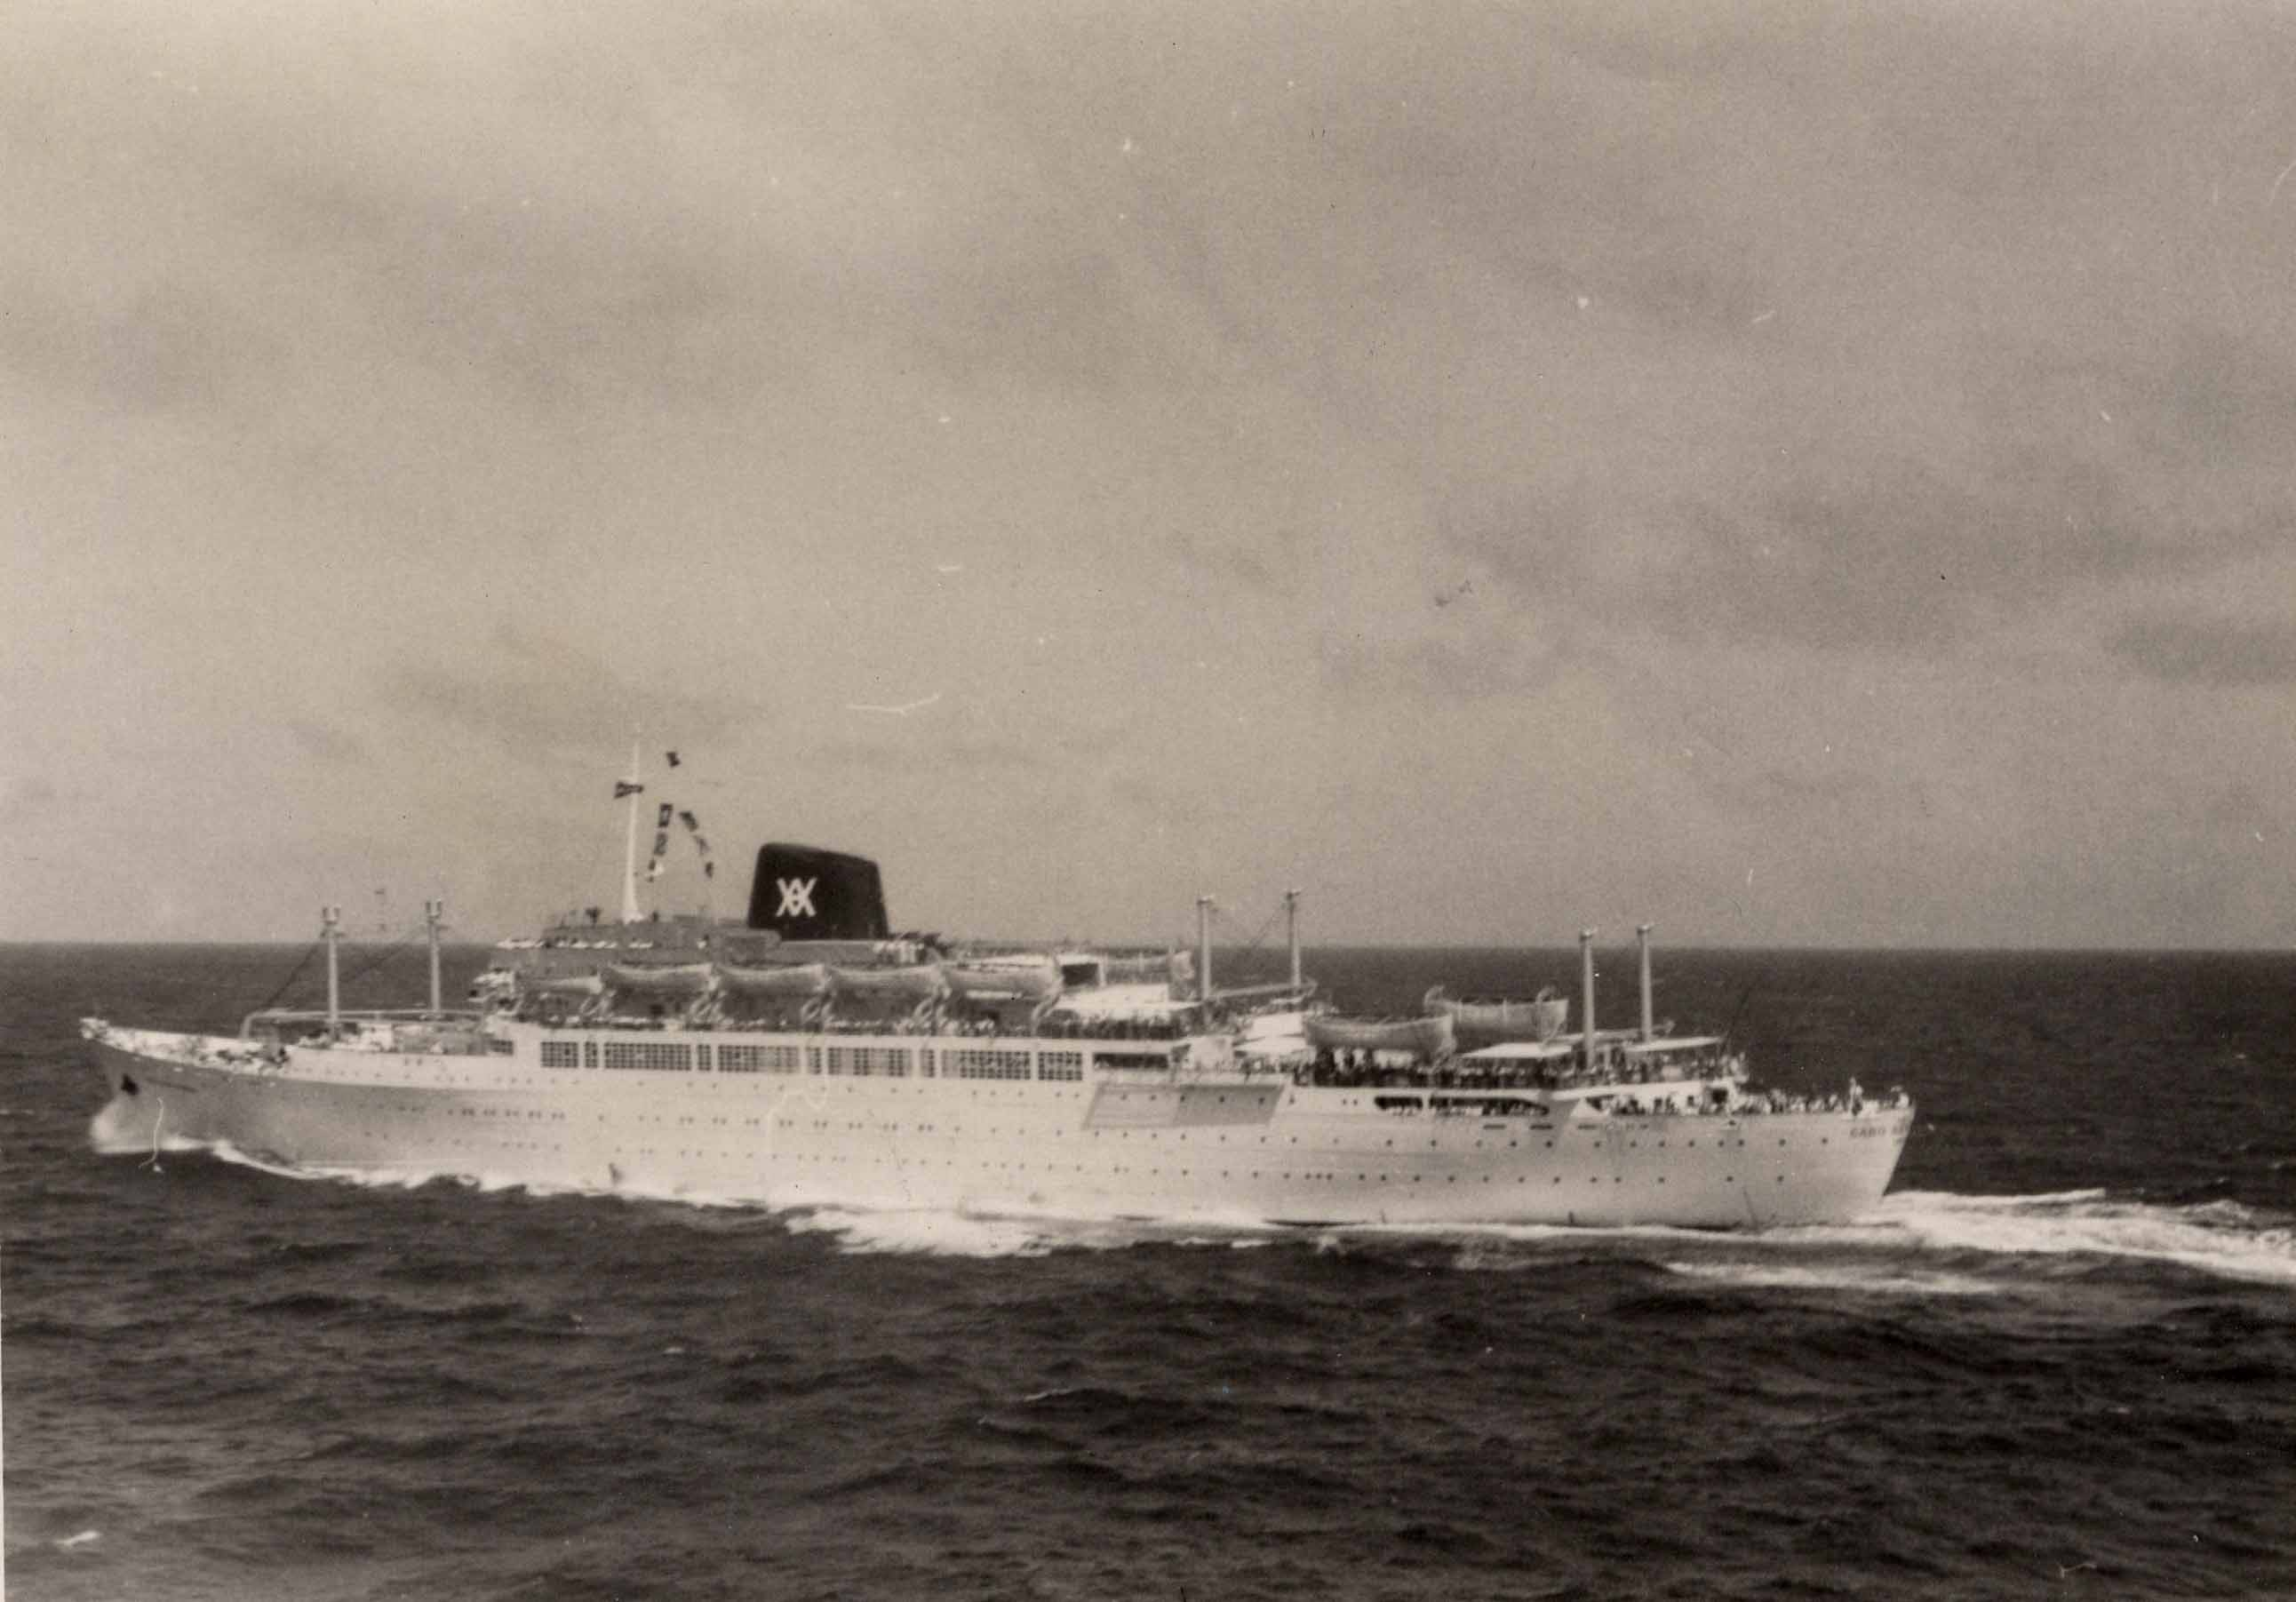
\includegraphics[width=4cm]{capa_diario.jpg}\par
        \vspace{4\baselineskip}
        {\Huge Diário de Viagem à Europa\\ \par}
        \vspace{2\baselineskip}
        {\Large 1959 \\ \par}
        \vspace{4\baselineskip}
        {\large\textsc{by\\[.5em]Othon Branco Baena}}
        \vfill
        Congresso Internacional de Esperanto\\realizado em Bruxelas\\[1em]
        {\em Baena Books}
 \end{titlepage}
 
\tableofcontents


\addchap{Julho}
\section*{07 \adfflatleafright \ISODayName{1959-07-07}}

A data de hoje há de ficar marcada para sempre em minha vida,  pois estou dando partida a um sonho que, até poucos anos atrás, parecia fantástico demais, para não dizer quase impossível: embarque para a Europa, e de navio, como eu sempre desejei.

A passagem estava primeiramente reservada no transatlântico italiano ``Federico C'', mas uma greve da tripulação prejudicou meu programa. O navio foi deixado parado em um porto africano e o jeito foi escolher outro, para evitar atraso nas escalas do meu estudado roteiro.

O agente de viagem que me deu assistência sugeriu, então, a transferência da passagem para o navio espanhol ``Cabo San Vicente'', que estaria fazendo sua primeira viagem à América do Sul. A princípio fiquei meio desconfiado, mas quando ele me passou um catálogo com descrição e fotos de todas as dependências do barco, concordei na hora. Assim, o atraso com a troca do meio de transporte, em relação à data da partida, foi de apenas dois dias.

Eis o bruto atracado aqui no cais da Praça Mauá, todo branquinho, no meio de intenso movimento de entra-e-sai. Minha mãe e quase todos os meus irmãos vieram ao embarque e também subiram a bordo. O navio procede de Buenos Aires, que é o seu final de linha, e vai nos levar até Gênova, na Itália.

Vou viajar em companhia de um antigo colega dos tempos de ginásio, o Alcino Beiriz, mas que só fui reencontrar no movimento esperantista. Há umas duas semanas ele apareceu no meu trabalho e, dizendo ter ouvido falar de minha viagem, lá na nossa Cooperativa Cultural, decidiu embarcar nas mesmas águas, desde que eu concordasse, é claro.

Meu plano de viagem inclui, até mesmo como ponto principal, a participação no 44º Congresso Universal de Esperanto, a realizar-se em Varsóvia, na Polônia, nos dias 1 a 8 de agosto próximo. Alcino se diz também esperantista, mas tenho cá as minhas dúvidas quanto ao seu real conhecimento do idioma internacional, pois jamais ouvi uma palavra em esperanto por ele pronunciada.

Descansando com o meu pessoal no salão-de-estar do navio, vislumbrei a um canto a conhecida vedete Rose Rondelli em conversa coloquial com Sérgio Porto, o apreciado cronista ``Stanislaw Ponte Preta'', do jornal ``Última Hora''. Mais tarde, ele desapareceu e ela, ao que tudo indica, será passageira.

A partida estava marcada para as 23 horas, mas sofreu enorme atraso. Logicamente, dispensei meus familiares muito antes. Consta que a causa da demora foi um interminável carregamento de café. De fato, vimos os guindastes despejando montes de sacos nos porões do navio.

Finalmente, beirando uma da manhã, o navio se pôs em movimento. A saída da Guanabara, naquela hora, mesmo assim nos permitiu um silencioso e emocionado ``Adeus, Brasil!''

O contato com os companheiros de viagem já se fizera facilitado desde os primeiros momentos da chegada ao cais. Isso porque lá encontramos, embarcada desde Santos, uma delegação brasileira ao Festival Mundial da Juventude, a realizar-se no fim do mês em Viena, na Áustria. Naquelas longas horas de espera, pude verificar que não são poucos, parece que em torno de cem pessoas, esbanjando mocidade, beleza e simpatia.

A primeira refeição, o jantar, por volta das 19 horas, com o navio ainda atracado, deixou logo agradável impressão, principalmente pela amplitude, conforto e beleza do salão. E, também, pelo enorme jarro de vinho tinto colocado na mesa, embora não tocado por mim\ldots Livrei-me, há pouco mais de dois anos, de uma manifestação alérgica de fundo presumivelmente alimentar e, por isso, decidi ficar, por algum tempo, longe de bebidas alcoólicas.

Fomos dormir às duas da manhã, já explicavelmente cansados, ante as peripécias do embarque. Além do antigo colega, travei melhor contato com os outros dois companheiros de cabine, a de nº 201: os semi-portugueses Srs. Noronha e Seixas, ambos já de meia idade e muito simples, gentis e camaradões.

\section*{8 \adfflatleafright \ISODayName{1959-07-08}}
A noite fez-se curta, mas foi bem dormida, pudera! Após uma breve acomodação ao balanço do barco, a cama confortável ``puxou'' rapidamente o sono. Ao amanhecer, entretanto, a disposição já era grande para o que desse e viesse.

O relógio precisou ser adiantado em 23 minutos, para ir se ajustando à hora legal. Depois do café, uma visita à coberta, para sentir a primeira sensação do mar alto, à luz do dia. O tempo ainda não estava muito firme, mas os prenúncios eram animadores e logo em seguida se confirmaram. A sensação, de fato, foi verificar a cor do mar, já longe da costa: azul muito carregado, ou melhor, azul-marinho\ldots

Outra interessante nova: pela fresta de porta do camarote distribuíram-nos, bem cedinho, o jornalzinho de bordo, de nome ``Maripez''. Bem impresso, com seis páginas, em formato tablóide e cheio de informações sobre o programa do dia e matéria ilustrativa geral. Belo e surpreendente trabalho.

De manhã dei um bruto ``fora'': entrei com o Alcino em um reservado de senhoras. Só percebemos na saída\ldots

Boas relações já fizemos com a turma do Festival da Juventude. Após o almoço, batemos longo papo com três paulistas (mãe, filha e sobrinha) e três dos vinte e tantos engenheiros espanhóis que estagiaram rapidamente no Brasil e estão de regresso. Começou o problema da língua: há que se falar espanhol.

Às 15 horas, como anunciado, um ensaio de salvamento em caso de emergência. Vestimos os salvas-vidas (coletes berrantemente abóbora) e seguimos as instruções afixadas atrás da porta da cabine: dirigir-se a um determinado local, quando soasse a sirene de alarme. O nosso ponto de deslocamento era o ``comedor'' (refeitório).

O cafezinho do bar ganhou o apelido de ``café milionário'' pois custa 4 pesetas (10 cruzeiros). É do tipo italiano, ``expresso'', mas a pequena xícara nem cheia vem\ldots

Afinal, este primeiro dia de viagem resultou bem proveitoso para a propaganda do esperanto. Já ficamos bem identificados como congressistas rumo a Varsóvia e isso tem despertado curiosidade e interesse por parte dos patrícios que se destinam ao Festival da Juventude. À tardinha, as três paulistas revelaram aparente disposição de conhecer maiores detalhes sobre o idioma internacional, notadamente a senhora, Dª Hilda, que pediu algum material que pudéssemos fornecer.

No jantar, sentaram-se à nossa mesa dois elementos da delegação ao Festival. Ao meu lado, o jornalista alagoano Jaime Miranda, olhando fixamente meu pequeno distintivo de estrela verde na lapela (insígnia do esperanto), criva-me de perguntas a respeito. Esclareço tudo como posso e ele também se foi, declarando que gostaria de conhecer melhor o assunto.

Às 21 horas, anima-se a festa no salão. A orquestra, no entanto, abusa dos ``paso-dobles'', gênero predileto dos espanhóis, mas assim mesmo dá para dançar. Não estreei ainda. Há excesso de cavalheiros, parece. Passamos depois ao cinema, no convés. Filme ``O Trem das 3,10'', com Glenn Ford e Van Heflin. O barulho da chaminé do navio perturba um pouco o som. A dublagem é em espanhol e impressionantemente perfeita. Mas naquelas condições perde-se muita coisa.

Quase às 24 horas, adiantamos o relógio mais 23 minutos, como se deverá fazer diariamente até o desembarque final.

\section*{09 \adfflatleafright \ISODayName{1959-07-09}}

Noite de profundo e repousante sono. Não encontro de manhã minha escova de dentes, que estava enfiada em um copo. O companheiro Seixas volta do banho e diz que, por engano, a usou. Paciência\ldots

O diário de bordo, o ``Maripez'', é entregue cedinho.

Esqueci-me de dizer que o jantar de ontem esteve magnífico: peru e champagne!

Pretendo estrear a piscina daqui a pouco. É pequena, mas dá para se divertir. O tempo segue maravilhoso. Limpo e de mar incrivelmente azul-marinho\ldots

Às 15 horas fizeram um bingo no salão. Não entrei porque caía de sono e fui tirar uma soneca, mesmo contra os meus hábitos. Dizem que o mar traz sonolência, no início, e parece que é verdade.

Um mapa nas laterais do passadiço mostra a posição do navio diariamente, ao meio-dia. Estamos na costa da Bahia, a 636 milhas do Rio e a 19 nós horários de velocidade.

Um nó corresponde a uma milha marítima, ou seja 1.800 metros, aproximadamente.

Hoje, 9 de julho, é a data nacional argentina. A sua delegação ao Festival de Viena é também numerosa, fora outros cidadãos em viagem com diferentes destinos. Às 18 horas reuniram-se no salão e cantaram o seu hino nacional. Eu não estava lá, soube pelos alto-falantes. Um ``drink'' foi oferecido aos presentes.

O chefe da delegação brasileira, radicado em São Paulo e naturalizado brasileiro, é espanhol. Soube que é proprietário do salão ``Antoine'', famoso cabeleireiro de senhoras da capital paulista. É, ainda, pai do laureado cestabolista Amauri, com quem aliás muito se parece.

Uma volta pela popa, às 19 horas, antes do jantar. Tempo estupendo. À esquerda (costa), a meia altura, um quadro curioso no céu: certa escuridão e uma fatia de lua brilhante, bem junto a fulgurante estrela, talvez a Dalva. Diz o Alcino, com muita propriedade: a bandeira da Turquia\ldots

Na direção da popa, bem visível, o Cruzeiro do Sul. Não há dúvida, estamos seguindo para o norte.

Após o jantar, mais festejo da data argentina. Um ``show'', no salão cheíssimo. Patrícios (deles) vieram da primeira classe para assistir. Recital de piano, excelente, pela mais brilhante executora de bordo, a brasileira Dona Clarisse. Depois, a bonita Nely, que deve ir representar nosso folclore em Viena, cantou ``Granadina'' e a toada gaúcha ``Prenda Minha''. A surpresa maior veio em seguida. O trio de rapazolas intitulado, parece-me, ``Maraiá'', vestido a caráter (chapéu de palha, camisa listrada verde-branco horizontalmente, calça clara) abafa sensacionalmente. Cantam cinco números. Vão desacatar no festival, sem nenhuma dúvida.

A bordo, mais tarde, um deles diz que são do Rio Grande do Norte e estiveram na TV Tupi do Rio e na de São Paulo. Sugiro-lhe que inclua em seu repertório, por muito se identificar com o estilo deles, a toada ``Vendedor de Caranguejo'' e ofereço-me para ensinar a letra.

Depois, finda o ``show''. Novamente o hino argentino, que termina falando em ``augurio murir com gloria''. Em seguida, o hino nacional brasileiro, após palavras inflamadas de agradecimento do representante argentino, uma grave figura.

Breve chuvisco atrasou um pouco o cinema. Filme: ``Mi Hermana Elena'' colorido, com Janet Leigh e Jack Lemmon. Refilmagem de velha comédia, ao que me lembre exibida no Brasil com o título de ``Jejum de Amor'', com Rosalind Russel e Janet Blair. História de duas irmãs pobres do interior que vêm para Nova Iorque morar em meio-porão devassadíssimo.

\section*{10 \adfflatleafright \ISODayName{1959-07-10}}

Manhã esplendorosa, como todas até agora. Escrevo sobre a perna, porque os salões só abrem às 10 horas. Estou na ``cubierta de paseo'', no convés, na parte mais traseira. Vou descer para voltar de short à piscina, que fica aqui junto mesmo.

Os companheiros de cabine são formidáveis. Discretos e educados. Dormem como anjos, sem o menor ruído. Hoje de manhã todos reclamamos contra a água dos chuveiros, que só estava saindo quente, quase fervendo.

Mais tarde, no salão, descubro que o pai do Amauri, o ``Antoine'', é de nacionalidade argentina e não espanhola.

O marido da cantora Nely, Sr. Armando Angelini, distribuiu o jornalzinho do Festival. Marcaram ensaio do hino deste, no salão. Participo da cantoria, que é vibrante. Em seguida, corre um páreo de ``caballos'', jogados com grandes dados e com apostas (25 pesetas) e tudo. É jogado no salão, em tapete próprio, marcado.

Para a noite está prevista a eleição de ``los reyes del ecuador''. Estamos, agora à tarde, nas costas de Alagoas/Pernambuco. O cruzamento do equador dar-se-á amanhã, conforme anunciam.

O cinema, após o jantar: ``La Venganza'', produção espanhola com o ator italiano Raf Valone e Carmen Sevilla. Teve prêmio em Cannes, no festival ao ano passado. Mas é um monótono drama de colhedores de trigo. Salva-se pelo colorido e alguns cenários.

No salão elegem a rainha do equador, uma argentina muito jovem, de pequena estatura. Em seguida o rei Netuno, o brasileiro Simão, movimentada figura da delegação ao Festival. Na mesma hora recebem faixas, coroas e, o rei, longas barbas e cabeleira. Dançam sozinhos a ``valsa da coroação''.

Estão programadas outras coisas para amanhã, às 10 horas na piscina.

\section*{11 \adfflatleafright \ISODayName{1959-07-11}}

Quarto dia de viagem. O diário de bordo, logo cedo, anuncia que cruzaremos o ``ecuador'' aproximadamente às 18 horas. E faz recomendações para que se evite excesso de exposição ao sol, pois a radiação é mais forte.

Marcam para as 10 horas o ``bautismo de los neófitos'', isto é, os que estão passando pela região pela primeira vez e que, nesta viagem, pelas conversas, são numerosíssimos --- maioria do pessoal do festival e muitos outros, inclusive nós dois\ldots

Fui convidado pela comissão de cultura da delegação brasileira ao Festival da Juventude para fazer uma palestra sobre o esperanto, na segunda-feira, às 16 horas. O jornalista Jaime Miranda já havia tocado no assunto antes e agora confirma. As palestras começam amanhã.

Netuno e sua majestática companheira comparecem pomposamente à beira da piscina, para os ``bautismos''. A chamada é feita nominalmente. Soube que só estão chamando os previamente inscritos na véspera, à hora das eleições dos reis, quando estivemos ausentes. Assim escapamos do vexame: um por um, ou uma por uma, frente às majestades, para umas boas pipocadas, na cabeça, de uma mistura branca, parecendo cuscuz, mas vim a saber depois ser sabão com sal. Em seguida, dois ou mais serviçais agarram o batizado e o atiram na piscina.

Dezenas e dezenas de ``neófitos'' cumpriram o ritual. Lá pelas tantas, os circunstantes foram aos reis e\ldots o banho foi geral. Depois a turma gostou do lance e durante mais de meia hora o programa consistiu no lançamento à piscina de pessoas vestidas, com cadeira junto, etc., etc., Felizmente o bom humor prevaleceu sempre. E felizmente também não se lembraram de mim, nem do Alcino e escapamos ilesos. Para isso concorreu naturalmente nossas freqüentes entradas espontâneas na água\ldots

Fotografias hoje. Fiz minhas primeiras O navio subitamente parou, por uns 15 minutos. Algum problema de máquina, talvez. Pouquíssima gente percebeu. Estávamos, porém na popa, fazendo a terceira catequese para o esperanto: Jeanete, jovem e gordinha, com sua mãe polonesa, em viagem para Israel. Como vamos estar na Polônia, ela se interessa. Naquela posição foi fácil perceber a parada do barco, pois desapareceu a esteira branca deixada por ele quando em movimento.

O ensaio do hino da juventude, pelos festivalistas, foi muito animado, pois o cântico é vibrante. A música é uma só, naturalmente, e cada país canta a versão no seu idioma. Participamos do ensaio gostosamente.

Na hora do jantar do primeiro turno (18 horas), que não é o nosso, passando pela porta do refeitório, quase caí para trás: todo o pessoal nas mesas --- e note-se que o salão é enorme --- ostentava fantasiais na cabeça, com chapéus os mais jocosos e extravagantes. Até o capelão envergava seu pitoresco gorro vermelho (!) de papel crepom. Como surpresa, nada mais hilariante.

Na nossa vez, encontramos os chapéus sobre os pratos virados. Eu e o Alcino ganhamos ``elegantes'' bonés, de imensas palas. Valeria a pena fotografar\ldots

Mais tarde, durante o baile com o pessoal fantasiado (pelo menos na cabeça) e o salão lindamente decorado, foi feita a entrega dos ``diplomas'' de travessia do equador aos neófitos.

Esta travessia aconteceu às 18h50m de hoje, quando o navio apitou repetidamente, em saudação. Assim, desde aquela hora já estamos no hemisfério norte.

\section*{12 \adfflatleafright \ISODayName{1959-07-12}}

O dia não amanheceu tão bonito.

Mas está ainda firme e promete melhorar bastante. Há ainda recomendações no jornalzinho ``Maripez'' para continuar o cuidado com o sol equatorial, muito intenso realmente. Mas o vento permanente da coberta alivia sensivelmente, pelo menos para mim.

Ao café, soubemos de um pequeno ``entrevero'' havido ontem à noite no baile. Fora servido um ponche com sanduíches, cerca das 23 horas. A turma do festival, ou melhor, alguns elementos já embalados pelas comemorações de Netuno, parece que andaram se excedendo.

Escrevo do convés --- ``cubierta de paseo'' --- ao lado da piscina. O balanço embora pequeno, combinado com o apoio precário sobre o joelho, sacrifica um pouco a caligrafia.

Aqui o barulho do navio se assemelha ao de um avião. É a pressão da fumaça da chaminé contra o vento ou a pressão atmosférica, segundo creio.

Hoje é o nosso primeiro domingo a bordo. Após o almoço, Creuza, da delegação do festival, faz uma palestra sobre este conclave, suas origens e objetivos. Explica que eles se realizam de dois em dois anos e sempre nos países da chamada ``Cortina de Ferro'', mas o deste ano, em Viena, será a primeira exceção. Muita gente na assistência. Depois, jogamos bingo, a 5 pesetas, no salão.

Seguimos nosso quinto dia de viagem, sem qualquer panorama externo senão o grande oceano, como sempre lindo e como sempre azul-marinho. No primeiro dia, cruzamos com um navio e passamos mais tarde por outro, ambos pequenos.

À noite, voltou o cinema: ``El Hombre de Laramie'', um faroeste com James Stewart. Já o havia visto há algum tempo no Rio, não sei sob que título. Muito boa dublagem, como sempre.

Na lateral da coberta superior, um dos rapazes do Trio Maraiá, o Hirton, ao violão, canta muito bem um sem número de canções, velhas e novas, numa rodinha muito simpática. Soam as 24 horas. Adianto o relógio mais uma vez em 23 minutos e vou dormir, pensando no jogo de hoje, lá no Rio entre Flamengo e Vasco, cujo resultado não sei quando descobrirei.

\section*{13 \adfflatleafright \ISODayName{1959-07-13}}

Como sempre, pela manhã, a piscina foi o ponto alto. Alcino, que não havia caído n’água desde o embarque, hoje se animou. O jornal de bordo marca para amanhã um baile de disfarces. Deverá ser curioso, pelos tipos que há a bordo. O navio fornece fantasias e outros apetrechos.

Às 12 horas o barco já se situava mais perto da costa africana. Passaremos, alta noite de hoje, pelas Ilhas Cabo Verde, pertencentes a Portugal. A chegada a Tenerife, nas ilhas Canárias, está marcada para depois de amanhã, ao anoitecer.

Escrevo no salão, em meio a certo tumulto. Aguarda-se a segunda palestra da série cultural da delegação do festival: médico brasileiro falará sobre o câncer. Talvez a minha seja a próxima, embora a data anteriormente marcada tivesse que ser revista.

Ontem de manhã lavrei um tento: conversando com duas argentinas e uma chilena, não se deram conta de ser eu brasileiro, a não ser quando eu disse! ``Tan bien hablas el castellano'', disseram-me. Imaginem\ldots

Descobri o significado da marca V e A, com as letras entrelaçadas, que formam a insígnia da companhia do navio, a ``Ybarra y Cia.'': ``vascas y andaluzas'', marca da marinha mercante espanhola, não sei de que época.

Observo o quanto trabalha o pessoal de bordo. Nos salões onde servem o café, após as refeições, apenas dois homens atendem, circulando por toda a imensa área. Nas outras horas, esses mesmos dois atendem a quaisquer encomendas, do bar ou não. Indago a um deles sobre o seu horário de trabalho. ``Das 8 às 24 horas!'' --- responde. E de manhã têm que estar a postos para ``limpiar'' as acomodações. Os músicos da orquestra, que são quatro, dão também sua mãozinha em outros serviços durante o dia. Já os vi limpando cinzeiros.

A palestra sobre o câncer alcançou grande interesse. O conferencista, Dr. David Herlich, do Instituto Central do Câncer, de São Paulo, mostrou competência e entusiasmo pela sua especialidade. Pertence também à delegação do Brasil ao festival de Viena e, em seguida, visitará os países socialistas, para maiores estudos.

Após o jantar, vejo no quadro a confirmação de minha exposição sobre o esperanto para depois de amanhã, quarta-feira, dia 15. Amanhã, um deputado estadual paulista, também da delegação ao festival, falará sobre questões de ensino.

O filme desta noite chamou-se ``Sinfonia en Oro''. É a história de um patinador que ficou incógnito como um certo ``Mister X''. Filme alemão, muito desinteressante, exibido no Rio há uns dois meses. Saí no meio e vim para o camarote alinhavar estas notas e dormir mais cedo.

Não sei se já falei sobre a excelência de nossas camas, com beliche e tudo. Espuma de borracha gostosíssima. E com ar condicionado no camarote, como, de resto, em todo o navio.

E assim se encerra nosso sexto dia de viagem. Já se fala em atraso de um dia, até Gênova, devido às escalas. Tudo ótimo!


\section*{14 \adfflatleafright \ISODayName{1959-07-14}}

É impressionante a calma do mar, desde a saída do Rio. Viajantes habituais, como o simpático português de nossa mesa de refeições, Sr. Guilherme, afirmam que nunca viram fato igual.

Às 13 horas, fomos ver a posição do navio no mapa. Passamos pelo arquipélago Cabo Verde durante a madrugada. Nada se viu. Anunciam que chegaremos a Tenerife amanhã, nas primeiras horas do dia. Já é mais freqüente o encontro com outros navios. Ontem, um pequeno pesqueiro foi avistado e identificado como do Senegal. Hoje, após o almoço, outro barco, este de maiores proporções e também de passageiros, navegava na mesma direção que a nossa. Horas depois sumia na imensidão do oceano.

A palestra, à tarde, foi também muito boa. O deputado estadual paulista, professor Solon, ocupou-se do tema educação. Finda a conferência, muitos debates, perguntas e respostas do palestrante. Achei, apenas, o conteúdo um pouco elementar. Lembre-se, porém, que a maioria do auditório era de estrangeiros.

Ao ser apresentado ao orador, para dar início à palestra, o jovem membro da comissão de cultura referiu-se à data de hoje, 14 de julho. E com boa ênfase exaltou-a, falando, inclusive, em queda de opressão, referindo-se, naturalmente, à data marcante da revolução francesa. Assunto delicado, pois nos encontramos neste barco, que é ``território'' da Espanha franquista\ldots É como se falar em corda em casa de enforcado.

O baile à fantasia excedeu a expectativa. Os recursos não eram muitos: cartão, papel crepom, tinta e cola. No entanto, surgiram ``disfarçados'' notáveis. Premiados: o rei Creso, que foi o marido da cantora Nely Angelini, e a ``Rainha do Egito'', a mesma graciosa argentina que já fora eleita rainha do equador.

Antes um pouco, membros da comissão de cultura chamaram-me para trocar idéias e planejar minha palestra de amanhã. Querem evitar que eu aborde o sentido universalista de fraternidade do esperanto, que pode cheirar a ``coisa'' e desagradar os franquistas.

\section*{15 \adfflatleafright \ISODayName{1959-07-10}}

Oito dias ao mar sem sequer avistar a terra de uma ilhota. Na próxima madrugada, finalmente, pisaremos em Tenerife.

A manhã está encoberta, sem sol, mas firme. Faltei à piscina hoje, antes do almoço, para esboçar minha palestra, que, já observei, está despertando certo interesse, pelos comentários de conhecidos. De fato, a propaganda está sendo maior (não de nossa parte) que a das anteriores. Talvez seja pelo assunto. Além do anúncio escrito no salão, o alto-falante de bordo repetiu o convite na hora do almoço. Poucos momentos antes da hora marcada, 15 horas, o Alcino estendeu no salão a bandeira e flâmulas do esperanto, que fazem parte de sua bagagem.

A afluência foi enorme, na verdade maior do que nas demais, e a sugestão de véspera, do simpático Dr. Maurício, da comissão de cultura, proporcionou magnífico efeito: convidou-se representante de cada nacionalidade presente a bordo para compor a mesa; havia portugueses, espanhóis, chilenos, argentinos, italianos (o vice-cônsul de Campinas), suíços, franceses, húngaros, sírios, libaneses, um belga, uma polonesa (mãe de Jeanete) e mais descendentes diretos que representavam Japão, Israel e União Soviética.

Cada um deles, ao chegar à mesa, cumprimentava-me dizendo ``boa tarde'' no seu idioma.

Pegando esse ``gancho'' da multiplicidade de línguas, passei em seguida a falar sobre ``A realidade do esperanto como língua internacional'' --- o tema oficial da palestra. Inicio desfazendo o clássico equívoco de que se esteja pretendendo suprimir todos os idiomas nacionais e substituí-los por um único; apresento um breve esboço histórico, uma demonstração do mecanismo da língua, sua extrema facilidade e a atual situação de penetração em todo o mundo. Recordo o caso da trabalhosa e demorada implantação do sistema métrico francês (também um projeto de unificação), que levou mais de duzentos anos para ser finalmente aceito. E, para não ultrapassar os 40 minutos programados, finalizo, para que a língua fosse ouvida, declamando a versão em esperanto que fiz do hino do festival da juventude, cantado quase todo dia a bordo.

O sucesso, modéstia à parte, foi estrondoso. Havia deixado a máquina fotográfica já preparada com o Alcino, para fixar a cena, com vista a uma futura publicação na revista da nossa Cooperativa Cultural.

Na forma usual, pus-me à disposição dos presentes para esclarecimentos e debates. Nas palestras anteriores, grande parte da assistência já se retirava nessas ocasiões. Surpreendentemente, hoje, ninguém se afastou e o salão permaneceu lotado por mais 30 minutos de informações e respostas, aproveitados por mim, então, para abordar aspectos que, por limitação do tempo inicial, haviam ficado sem referência.

Ao encerrar, um grande grupo se acercou da mesa e levou todo o material de propaganda e folhetos disponíveis. E me arrancam a promessa de, ainda a bordo, até o fim da viagem, ministrar algumas aulas elementares. O chefe da delegação ao festival, o animado Antoine, fala no encerramento, exaltando o assunto objeto da palestra e cita, a propósito, sua experiência de dois anos atrás, em Moscou, quando durante 45 minutos conseguiu ``não entender'' nada do que o motorista de um taxi, com quase obstinação, lhe desejava transmitir. A barreira das línguas!

Não há dúvida de que fizemos, nesta tarde, um servição pelo esperanto, semeando em excelente terreno.

\section*{16 \adfflatleafright \ISODayName{1959-07-16}}

Foi notável a chegada a Tenerife, em sua capital Santa Cruz de Tenerife, nas ilhas Canárias, pertencentes à Espanha. Havíamos ido dormir a uma da manhã. A chegada deu-se às três e a quase totalidade dos passageiros desembarcou imediatamente.

Os oito dias em mar alto assim o exigiam. Eu queria dormir mais, pois o navio iria permanecer neste porto até as 13 horas. Mas às 4,30 tive de seguir o exemplo dos companheiros e, escuro ainda, desembarcar. A cidade estava, porém, cheia de movimento, com o comércio todo aberto! E táxis em profusão no cais. Ainda a bordo somos ``assaltados'' por vendedores de uma infinidade de coisas.

Tenerife é porto livre, isto é, sem alfândega. Há de tudo. Os preços nos assustam, mas no bom sentido. Um cálculo rápido ``peseta-dólar-cruzeiro'' e verificamos que é quase tudo pela metade dos preços no Brasil.

Tomamos café em mesas ao relento, escuro ainda. A limpeza das primeiras ruas e praças avistadas é impressionante. Carros-pipas estão lavando os calçamentos, com homens esfregando vassourões.

Exploram-nos neste café, pão-manteiga e ``toddy'' para quatro pessoas: 48 pesetas, ou seja Cr\$150,00! Não deixamos gorjeta\ldots

Corremos as lojas. Vários negociantes hindus, pois há uma regular colônia deles nas Canárias. Rádios-transístores e relógios suíços e alemães baratíssimos. Mas não me interesso em adquirir nada, a não ser ``souvenirs''. Inconveniente fazer bagagem tão cedo. Ficará para a mesma escala, na viagem de regresso.

Clareia, finalmente, e a cidade se agita com rapidez. Os perfis das casas espanholas, interessantíssimas, se projetam melhor. A pavimentação é impecável e os serviços de transporte exibem ônibus grandes e numerosos, rodando em todas as direções. Nossa surpresa é enorme. Carros de todos os tipos, europeus na quase totalidade, moderníssimos em maioria.

Batemos nossas primeiras fotografias em terra firme, já encontrando, por acaso, os companheiros de camarote, Noronha e Seixas. Vamos ao grande mercado ``Nuestra Señora de África''. A edificação é maravilhosa, ampla, espaçosa e limpíssima. O movimento é muito grande, mas o sortimento é superabundante. Compramos um quilo de uvas pretas: 10 pesetas (Cr\$25,00).

Um ônibus nos leva a Laguna (San Cristobal de Laguna) local de nascimento do jesuíta José de Anchieta, figura importante da nossa história antiga. É outro município, mas a continuidade urbana une praticamente os dois. A casa onde nasceu Anchieta é muito visitada. Mesmo em Santa Cruz vejo um templo de aspecto secular, restaurado e caiadinho de novo e que deve ser do tempo do apóstolo. Está justamente na ``Calle (rua) José de Anchieta''.

De volta, Alcino, em uma loja de livros, revistas e jornais, obtém informações sobre um esperantista de Tenerife, de nome Régulo Perez. O homem da loja, gentilmente liga para ``Juanito'' --- como o chama --- e com ele converso pelo telefone. Marcamos um encontro, mas ele tarda demais. Enquanto isso conversamos com um bando de ``pibes'', na praça. Sabem que o nosso dinheiro se chama ``cruceiro'' e que a capital futura do Brasil é ``Bracília''\ldots

E muitos deles conhecem várias palavras em esperanto, o que nos surpreende. Bom trabalho dos esperantistas canarienses. Deixamos recado e indicação do navio para Perez e voltamos para bordo, a tempo de alcançar o almoço. A largada está marcada para as 13 horas e acontece com pequeno atraso.

Depois soubemos que um senhor com estrela verde na lapela tentou subir a bordo, mas as escadas já estavam içadas.

Afastamo-nos de Tenerife, cujo cais, muito bom, está cheio de navios, na maioria espanhóis mesmo. Fotografo alguns ângulos.

Este primeiro contato com uma população ``extra-brasileira'' espantou-me bastante. Quantas qualidades boas, na parte material e na pessoal! O povo pareceu simples e gentil. Nenhum vendedor mostrou mau humor por não se comprar nada, depois de ver e indagar muito. Numa farmácia de Laguna, entramos quatro só para tomar o peso; era daquelas balanças antigas de correr pesinho. O homem pesou todos nós, atenciosamente, e continuou sorridente aos nos despedirmos sem nada comprar ou deixar gratificação.

O tráfego tão silencioso, sem algazarra de buzinas ou de pedestres, dá grande e benéfico alívio aos ouvidos.

Assim senti Tenerife. Pouco depois, mar alto outra vez, caí na cama para dormir o sono faltado na véspera e compensar as canseiras da escala.

Após o jantar, a delegação brasileira promove novo ``show''. O baixo (cantor) até então inédito a bordo, faz sua estréia em grande estilo. Depois, a bela Nely Angelini, Clarisse Leite, a esplêndida pianista, e Magali, a paulista de sorriso tipo anúncio de creme dental, recita Bilac; Luiz Vergueiro, também paulista, diz um monólogo jocoso. Por fim o fabuloso Trio Maraiá, que abafa como sempre. Estou louco para ver esses três se exibindo em Viena.

A chegada a Lisboa está marcada para depois de amanhã, cedo, às 6 horas, dizem.

\section*{17 \adfflatleafright \ISODayName{1959-07-17}}

Bem recuperados, lamentamos não poder voltar à piscina. O tempo está firme, mas sem sol e venta fortemente na coberta.

Desço para alinhavar estes comentários, pois a vontade de levar o diário até o fim agora é grande. Não sei se sairá.

Hoje é sexta-feira. O jornal de bordo, em seu noticiário telegráfico, nada disse das disputas esportivas do Rio. Ainda não sei o resultado de Flamengo x Vasco, do dia 12.

De agora em diante, as escalas serão diárias: Lisboa, Tanger, Algeciras (junto a Gibraltar), Barcelona (dia e meio), Marselha e Gênova.

Inscrevemo-nos na excursão organizada pela companhia do navio, durante a parada em Lisboa, amanhã, onde devemos aportar às 6 da manhã. O passeio custará 250 pesetas, mas durará 4 horas. O navio ficará até as 3 da tarde.

Nossos dois companheiros de camarote, os excelentes Noronha e Seixas, ficarão em Lisboa. Também os companheiros de mesa, Sr. Guilherme, D.ª Margarida e a filha, Irene, descerão lá.

Realiza-se, agora, outro ``show'' no salão, este justamente oferecido pela delegação brasileira aos portugueses que se ``quederán en su tierra''. Vou para lá. Acabo de escrever longa carta à Cooperativa Cultural dos Esperantistas, dando as boas notícias dos acontecimentos de bordo. Para casa já havia escrito à tarde. E ainda fui obrigado a refundir o noticiário que o Alcino preparou para ``O Jornal'', do Rio.

\section*{18 \adfflatleafright \ISODayName{1959-07-18}}

A chegada à Lisboa foi maravilhosa.

Acordei às 6 da manhã e os nossos dois companheiros já estavam prontos e com tudo arrumado. Avisaram que ainda faltava um pouco para atingir terra. Vesti-me e subi para a coberta lateral, com o binóculo. Amanhecia o dia, ainda cheio de névoa. Dali a pouco uma nesga de terra fez-se visível --- minha primeira visão da Europa!

Mais um pouco e mesmo a olho nu se divisavam contornos à direita e à esquerda; no meio, a barra do rio Tejo, muito larga. Com o binóculo percebo que a aparente torre da direita é o novo monumento a ``Cristo Rei'', em Almada, frente à Lisboa. Vagarosamente vamos vencendo a barra, que me surpreende pelas águas verdes e claras como o próprio mar.

O dia levantou-se exuberante. Atracamos às 9 horas, mais ou menos. Antes fotografei a lendária Torre de Belém, menor do que eu supunha, mas clarinha e bem conservada. Às 10h30m saímos em excursão de três horas e meia, em magnífico ônibus, com cicerone e sistema de som interno.

O guia fala espanhol. Da zona do cais ganhamos o centro, rua Augusta (das principais do comércio), Rossio (com o monumento ao nosso Pedro I, aqui Pedro IV), Avenida da Liberdade, a principal e que impressiona pela largura, pavimentação impecável, arborização e ajardinamento notavelmente florido.

Tráfego fácil e silencioso. Carros modernos de dezenas de tipos, mas europeus. A cidade não é plana; pelo contrário, assenta-se em colinas, em número de sete, esclarece o guia. As subidas lembram São Paulo. A patrícia Laís, paulista, como praticamente toda a delegação ao festival, senta-se ao meu lado e acha a fisionomia daquele trecho final da Avenida da Liberdade parecida com Montevidéu.

Dali vamos parar no Palácio de Queluz, onde nasceu Pedro I, mas que está fechado para recepcionar, hoje ou amanhã, Hailé Selassié, imperador da Abissínia. O palácio é baixo, róseo e está bem descascadinho, esparramando-se amplamente para os lados.

Dali tomamos o rumo de Sintra, fora de Lisboa, mas bem perto, junto à serra do mesmo nome. Pelo caminho, sempre muito bem asfaltado, vejo vegetação amarelada, morros pelados, de terra com saibro, aquedutos (um subterrâneo, com respiradouro somente aparecendo), moinhos em ruínas. Sintra é um pequeno bosque, de tão arborizada. Ali viveu o poeta Lord Byron (o guia aponta a casa), que lhe cantou as delícias.

As ruas, subindo pelas raízes da serra, são estreitíssimas. Paramos à porta de seu monumento máximo: o castelo mourisco, que visitamos cômodo por cômodo. Depois um lanche no acolhedor bar do Hotel Paris. Fotografei o interior do castelo, minha primeira velharia penetrada na Europa, e permutei poses com o Alcino, à frente do mesmo.

Olha-se em torno, e da mata fresquíssima pontificam torres de castelos. Lá no cimo, duas fortificações do tipo medieval, que também fotografei, e torrinhas menores de construções mais particulares.

Pagamos o lanche em pesetas. O rapaz, nosso primeiro contato a sós em Portugal, fez conta, refez e descobrimos que ia se enganando em 100\% contra nós\ldots

Boa caminhada dali a Cascais, uns 20 quilômetros, ganhando-se a costa. Somos apresentados ao cabo de São Roque.

As dunas da praia dos Guinchos cospem areia e o forte vento fá-las guinchar mesmo, ruidosamente. A costa é toda pedregosa, de lavas vulcânicas. O vulcão era em Sintra e inundou toda a região até quase junto a Lisboa.

Cascais é lugar de endinheirados, com majestosas casas à beira-mar. Mora ali o rei Humberto, da Itália, que comprou um palacete, alugou-o e passou-se para um antigo e enorme palácio ao lado. Antes um pouco de Cascais, a ``Garganta do Inferno'', vão aberto na alta pedraria vulcânica, muito profundo, fazendo um arco natural, através do qual o mar penetra um pouco terra a dentro. Bonito.

Cascais tem também um iate-clube. Mais adiante, o famoso Estoril. O conjunto é fabuloso nas cercanias do cassino, cujos jardins são magnificentes, hotéis, termas e balneários. Mas a praia é ridícula, dois palminhos de areia escura e de mar parado. Aliás, as outras todas não vão muito além.

No caminho de volta à Lisboa vêm, em seguida: Carcavelos (a maior e melhor praia), Oeiras e Passo d’Arcos. O mar é verde e limpo. Mas a faixa praieira é estreita e de cor pardacenta. E todas elas espetadas de armações verticais, alinhadas em toda a extensão da areia: as barracas. Aluga-se o pano e cobre-se a armação. Feíssimo!

Rumamos de volta a Lisboa. Fortes maiores e menores, à beira-mar. Um deles, baixo e compacto, foi adaptado para residência estival de Salazar, o governante português. Hoje ele não está --- diz o guia, pois não se vêm guardas à entrada.

Lembro-me de que hoje é sábado e já passa das 13 horas. Aqui deve ter também uma ``semana inglesa''. O tráfego de automóveis é agora intenso. As praias já mostram um bom movimento de banhistas.

A Torre de Belém, outra vez, agora de trás e de terra, vista de pertinho. Outrora ficava isolada no mar, a quase quilômetro e meio da terra. Os aterros fizeram-na, agora, junto da extensa via beira-mar. Caminho de ferro, eletrificado, como todos os outros que vi, passa também junto.

Um desvio à esquerda para rápida visita ao Estádio Nacional, o tal de gramado divinamente franjado claro-escuro. Uns tons de verde alucinantes. Está vazio, é claro. Homens cuidam do ``relvado''. O estádio é quase todo de pedra clara e decorado, em alguns pontos, com paredões em colunas, retangulares ou arredondadas. Batemos chapas e vamo-nos.

Quase ao voltar ao cais, passamos pelo castelo dos Jerônimos, aliás mosteiro. Belíssimo, no estilo chamado ``manoelino''. O tempo não permitiu, porém, visita ou simples parada à porta. Ficará para a volta à Lisboa, no fim desta viagem.

Almoço a bordo, já quase às 14 horas. Ficaram em Lisboa mais de duzentos passageiros. Tentamos um telefonema para um esperantista local. Linha ocupada seguidamente. Como não temos escudos, pago uma revista em pesetas e reembarcamos. Fico sabendo que também desembarcou aqui a vedete Rose Rondelli, que, durante a viagem, foi sempre vista rodeada de cavalheiros, espanhóis e argentinos.

Nota pitoresca: dez passageiros se atrasam e ficam em terra após o desencosto do navio. Vieram para o largo em um rebocador e embarcaram debaixo de estrondosa mas amistosa vaia, comandada pelo Antoine.

Quase às 16 horas, estamos deixando a barra do Tejo, rumo a Algeciras, pequeno porto espanhol pouco antes de Gibraltar. Revemos toda a orla de cada margem do belo e limpo rio. Interessantíssimo que suas águas não se misturam com o mar até a embocadura, em cujo meio há um farol; vê-se nitidamente a linha divisória, em tons diferentes de verde.

Até mais tarde, Lisboa, que tanto nos encantou! Alinhavei de uma penada todas estas minhas primeiras impressões. A Europa já começa a exceder a expectativa. Um detalhe ressalta em Portugal, aliás dois: a vida parece calma e organizada; e os automobilistas são verdadeiramente felizes, com tão maravilhosas ruas, avenidas e estradas.

Última recordação de Lisboa: as mulheres carregadoras de areia do cais do porto. Transportam até 60 quilos, em cestas ou latas sobre a cabeça, caminhando por uma estreita tábua, dos barcos (espécies de pesqueiros com ponteiras fenícias) à margem.

Leio mais tarde, na revista que comprei, intitulada ``Diário Ilustrado'', que Maysa estreará hoje no Cassino Estoril. E no mesmo órgão leio também que não há semana inglesa em Portugal, pois agora é que se está cogitando de introduzi-la.

São nove e meia da noite e ainda está claro. Pouco mais tarde passamos pelo Cabo de São Vicente, a beiradinha sul de Portugal. Agora já está escuro e a luz giratória do seu farol chama a atenção. Devemos atravessar Gibraltar às 5 da manhã e chegar a Algeciras, na Espanha, lá pelas 6. Soubemos com pesar do cancelamento da escala em Tanger, no Marrocos. Era a minha única oportunidade de pisar em solo africano. Será verdadeiro o boato?

\section*{19 \adfflatleafright \ISODayName{1959-07-19}}

Ontem mesmo, à noite, desfazia-se a dúvida, aliás mal entendido, quanto à parada em Tanger, que estava confirmada. Logo cedo, o ``Maripez'' noticiava os horários. Não consegui acordar na hora em que pretendia para assistir a passagem pelo penhasco de Gibraltar, ou seja, a travessia do estreito que marca a entrada no mar Mediterrâneo.

Mas o horário anteriormente falado não fora vencido como previsto. Às 8 e pouco atingíamos o porto espanhol de Algeciras, nossa primeira visão das terras ``franquistas''. É uma bela baía, no estreito, mas antes de sua parte mais apertada, onde se acha o penhasco, com as fortificações inglesas. Do lado oposto, a costa africana.

O estreito não é tanto assim. Na altura de Gibraltar tem uma largura de uns vinte quilômetros. Fora dali, muito mais. Mas durante a travessia a vista domina inteiramente os dois continentes, que tem costas algo elevadas, com profusão de penhascos e montes. Algeciras não dá acesso a grandes vapores. Por isso ficamos ao largo. Desembarcaram os passageiros com destino a Madrid, entre eles os engenheiros espanhóis que estagiaram no Brasil. A cidade é pequena e encarapitada na elevação do terreno. De binóculo vasculho tudo. O ``Hotel Santa Marina'' e a ``Cerâmica Virgem de los Milagros'', com grandes letreiros nas fachadas. Divisamos, na beira-mar, em apertada pracinha, ônibus e bondes.

A baía é realmente bonita. À direita, fechando-a bem, fica Gibraltar, que, no momento, está sob densa névoa em sua parte baixa. Não se distinguem bem as fortificações, mas os vasos de guerra ingleses lá estão abrigados, em bom número.

Duas horas mais tarde, largamos rumo a Tanger, isto é, retrocedendo pelo estreito. Então passamos bem junto de Gibraltar. Face à névoa, deixo de fotografá-lo, preferindo fazê-lo na volta, hoje mesmo, quando passarmos a caminho de Barcelona.

À hora do almoço, Tanger está à vista e causa sensação. Muito grande, com elevações amontoadas de casas estilo árabe, como se fossem uma só; deve ser a parte velha, a muçulmana. À esquerda, enorme e bela praia, a primeira que vejo capaz de rivalizar com as nossas. Ao centro, perfis de altos e modernos edifícios.

Almoçamos, apressados, enquanto o navio encosta e se cumprem as formalidades de praxe, antes do desembarque. Ao subir do refeitório, já encontro o navio encostado. Lá embaixo, uma quase feira livre de vendedores de mil coisas para os passageiros. Tanger também é porto livre, sem alfândega. Avisto os primeiros muçulmanos de trajes típicos, com e sem fez (chapéu rijo, sem aba); e a primeira mulher de longas vestes escuras, com o rosto coberto! Fotografo-os, discretamente, lá de bordo mesmo.

Depois descemos e nos dão duas horas para ir à cidade. Foi o máximo da viagem até agora! Embrenhamo-nos a pé, pelo bairro muçulmano, o lendário Casbah, dos filmes de ``intriga internacional'' e mistérios orientais. Percorro as ruas estreitíssimas, sujas, lojinhas minúsculas, mal-cheirosas, paredes seculares. Um autêntico mundo árabe. Um rapazola, com muita mímica, resolve se candidatar a nosso cicerone.

O primeiro elemento típico, de trajes árabes e montado de lado em minúsculo jumento me encontra de máquina em punho para fotografá-lo, mas --- grande decepção --- ele faz gestos enérgicos de protesto, além dos gritos, e não me animo a bater as chapas. Verifico, então, que não admitem ser fotografados, por motivos de tradição, religião ou dignidade. Há que disfarçar e, para isso, posamos nós próprios, com eles desatentos em segundo plano.

Predomina a pobreza franciscana, com oscilações até a miséria, pois são muitos os sentados aos cantos das quase intransitáveis ruelas. Mulheres de rosto coberto cruzam a todo momento.

Numa loja compro um fez por 50 pesetas. É só regatear que os preços caem verticalmente. Vamos até a parte mais alta. Há um velho castelo de algum lendário sultão, todo decorado no característico estilo mourisco. O pátio interno, infalível em toda edificação árabe, está florido, mas o aspecto de abandono da velharia, castigada pelo tempo, é inevitável. Mais um pouco e atingimos a beira-mar, lá do alto. Há uma amurada, do complexo arquitetônico que é aquilo. Abaixo, na pedra, a uns três metros, um árabe esta curvado, certamente em orações; levanta meio corpo e põe outra vez a testa sobre uma curta esteira. Por prudência (e, em parte, respeito) escuso-me de fotografá-lo.

Descemos pelo interior de um cabaré, àquela hora vazio, naturalmente. Tapetes de esteirinhas e almofadões no chão, em torno das paredes, nas várias saletas. Mesinhas miúdas em outras, que devem ser os bares. Neste mesmo grupo, uma sacada para o mar, bem elevada. Vista magnífica. Batemos várias chapas. E toca a percorrer labirintos de fazer medo.

Juntamo-nos a outro grupo do navio, com um guia local, em trajes típicos, falando bem espanhol. Leva-nos a um canto de um pátio ensolarado, onde dois velhos árabes ostentam cestas do tipo porta-serpentes. Excitamo-nos ante a perspectiva de presenciar um autêntico ``encantamento'', pois duas cobras são postas para fora. Os dois executam uma dança saltitante, acompanhada de cantoria puxando para choramingo, mas nada de flauta nem de encantamento. Pegam as cobras e fazem com que elas mordam seus narizes! E depois a língua! As moças dão gritinhos de susto --- ou de nojo. Fotografamo-nos ao lado deles, como uma bela recordação\ldots

A estranha sensação de Casbah faz-nos desistir de percorrer, em giro de táxi, a cidade moderna. Valia mais a pena ficar por ali mesmo. Há trechos de comércio predominantemente espanhol, como se vê pelos nomes das lojas (lojinhas, algumas de pouco mais de dois metros quadrados) em castelhano, e em árabe por baixo.

Fizemos mais compras, em lojas e no meio da rua, com camelôs. Tudo nos parece baratíssimo e o preço pago é, às vezes, menos da metade do inicialmente pedido.

Três ou quatro companheiros de viagem, uma moça entre eles, entraram inadvertidamente numa mesquita. Foram, por assim dizer, escorraçados e ouviram falar que muita sorte tiveram, pois a falta fora gravíssima, não raro caso de morte. A moça teve ainda a ousadia de bater uma chapa lá dentro!

Disseram eles que o interior é soberbo, arquitetônica e decorativamente, e que não tem nenhum móvel, somente esteiras e almofadas. Passamos na porta dessa mesquita. Alguns fiéis, plantados em vários degraus de escada acima do nível da rua, olharam-nos friamente. Não sei se naquela hora já havia ocorrido o incidente.

Voltamos quase correndo para o navio, pois que em cima da hora marcada para a partida. Um longo silvo soou, enquanto vínhamos a caminho. Junto do vapor a feira livre fervilhava. Compro dois lenços para cabeça, típicos, como ``souvenirs'', e, em seguida, resolvo me interessar por rádio transistor, que os havia maravilhosos. Peço preço. ``Que moneda, señor?'' --- arranha o vendedor. Falo em dólar e ele pede 35; faço um simulado espanto, digo que o navio já vai partir e exibo uma nota de 20, adiantando que era o que possuía. E saio na direção da escada. O coitado por aquele preço não poderia vender mesmo (seriam Cr\$2.700,00), parece-me, pois implorou longamente para chegar aos 25; se oferecesse 23 ou até 22 mesmo eu traria o rádio. Mas a vontade de comprar era nenhuma e ficou tudo por aquilo mesmo. Só fiquei com pena do homem e me arrependi do que fiz. Em Tenerife, na volta, poderia fazer melhor negócio.

Deixamos Tanger e duas horas mais tarde voltamos a cruzar Gibraltar. Por azar meu, passamos mais junto da costa africana. E a bruma é ainda pior que a da manhã. Quando passava um pequeno petroleiro, bato a chapa só para documentar.

À noite senta-se à nossa mesa, para jantar, um casal marroquino, com duas filhas, Anne e Gislene, de uns 13 ou 14 anos. São brancos, como a maioria dos marroquinos, e falam francês. Anne, a mais velha, fala um pouquinho de inglês. É uma tortura mental nossa conversa e, tomado de surpresa, tenho de arrancar de chofre, da memória, todo o meu francês.

O Alcino merece o ``prêmio Nobel'' da ignorância e negação pelas línguas. Não consegue guardar absolutamente nada e se mostra incapaz de aprender sequer uma palavra. Cabeça ruim está ali\ldots Como se não bastasse, insiste em tagarelar em português, sem se dar conta de que ninguém ``pesca'' vintém\ldots Solta uma longa frase. Os marroquinos sorriem amarelo e se voltam para mim, silenciosamente indagadores. Tenho que me virar para traduzir, de algum modo, o que o falastrão botou para fora.

Após o jantar, sentamo-nos outra vez com eles para assistir o ``show'' da delegação brasileira oferecido à Espanha e aos espanhóis que amanhã desembarcarão em Barcelona. Foi o mais fraco de todos. Mas, felizmente, para encerrar, o Trio Maraiá chegou e, como sempre, empolgou.

O cinema do convés caiu verticalmente. Depois das 9,30 da noite o vento lá fora é insuportável.

Amanhã à noite atingiremos Barcelona, onde a parada será a mais prolongada, talvez 36 horas. Assim, o atraso do navio chegará a dois dias e só no dia 23 chegaremos a Gênova, e não no dia 21, como previsto.

\section*{20 \adfflatleafright \ISODayName{1959-07-20}}

Tempo magnífico, como, aliás, desde a saída do Rio, há 13 dias atrás. A costa espanhola está sempre visível à nossa esquerda. É toda ela agreste, pedregosa.

Da piscina venho assistir um pouco o panorama, da amurada. O espanhol ``boa praça'', Sr. Bernardo de Castro, há trinta anos no Brasil, me identifica a cidade que se delineia pendurada na base de um penhasco: Alicante, junto do Cabo de Santo Antônio.

Já passamos pelo Cabo de Palos, de onde partiu Colombo para descobrir a América. Agora nos afastamos mais da costa porque --- diz o Sr. Bernardo --- há muitos recifes dali por diante. Esse espanhol foi o pioneiro no Brasil da fabricação de redes para pesca, e hoje domina todo o mercado nacional. Mora, ou melhor, tem família em Fermoselle, província de Zamora, fronteira com Portugal. Já nos deu o endereço e combinamos um encontro nas festas de Salamanca, quando voltarmos, em setembro.

Com a luz do sol se pondo às 21 horas, acercamo-nos de Barcelona. O crepúsculo estava espetacular, purpurino, cobrindo as colinas que se estendem até a região central da cidade. Mas ainda temos uns 30 minutos de navegação até o cais. Do lado contrário, uma lua monstruosamente cheia, no céu claro ainda para anoitecer. Quase 400 passageiros --- soube depois --- ficarão em Barcelona. O ambiente é festivo, quase de agitação. O alto-falante de bordo toca ruidosamente melodias marciais.

A chegada foi, assim, algo apoteótico. Ao acostar, não sei de onde saíram tantas serpentinas. O barco espanhol, orgulho de sua marinha mercante, completava, no território pátrio, sua primeira viagem! Cais atulhado de gente. Enfim saltamos, lá para as 22h30m horas. As luzes da cidade já haviam dado uma idéia de sua enorme extensão, com seu milhão e meio de habitantes.

Conhecemo-la, assim, primeiro à noite. E teremos o dia inteiro de amanhã para rodar, pois o navio partirá às 22 horas.

A impressão foi magnífica. Logo ao lado do cais a Plaza Colón (Praça Colombo), com o famoso monumento ao descobridor, que está lá em cima encarapitado, apontando para a América. Depois a Ramblas, avenida estreita nos lados, para o tráfego, e com larguíssima calçada central para o ``paseo''. Excelente arborização, bares à margem e, ali mesmo, estações do ``metrô'', que eu nem sabia que existia.

O movimento é intenso, apesar da hora e de se tratar de uma segunda-feira. A avenida é longa. À esquerda, várias ruelas estreitas levam aos trechos mais antigos e típicos. Um popular nos aborda, talvez atraído pela insígnia ``Brasil'' no nosso peito. Recomenda-nos uns ``nightclubs'' e o lado antigo, como curiosidade.

Passeamos até a Plaza Cataluña. No caminho, mais duas estações do ``metrô'': ``Fernando'' e ``Liceo''. Em um bar --- ``Granja Royal'' --- tomamos um bom leite, com excelentes pãezinhos, puxados a pastelaria. Dobramos a dose. E conversamos com o garçom sobre o preço de açúcar e Evaristo, futebolista brasileiro que alcança grande sucesso em Barcelona. O açúcar vem num saquinho de papel com dose certa. O preço do lanche é caro: 56 pesetas (Cr\$180,00, mais ou menos).

Voltamos para o lado da parte antiga, onde há até um bairro chinês. O ambiente ali é pesado, a freqüência suspeita. O ``nightclub'' recomendado era ali, o ``Jardim de Granada''. Senta-se ou no bar, em altos bancos junto a um balcão (45 pesetas), ou nas mesas ao ar livre (90 pesetas). O ``show'' musical é, porém, muito bom, pois tipicamente espanhol, uma vibrante flamenqueria, regada a fartos ``óles''.

Giramos por outras ruas. E falamos (menos Alcino\ldots) bom espanhol com outros tipos, que elogiam nossa linguagem e pronúncia --- curso de 15 dias a bordo\ldots

Uns companheiros de viagem, encontrados por acaso, reclamam contra o pagamento de uma taxa, porque sentaram-se em poltronas de madeira, na Ramblas. Mas tinham direito de ficar até as 6 horas da manhã, informou o funcionário cobrador\ldots

Voltamos bem tarde para o navio, de táxi. É, aqui, uma condução relativamente barata.

\section*{21 \adfflatleafright \ISODayName{1959-07-21}}

Ficaremos o dia inteiro em Barcelona, pois a largada dar-se-á às 22 horas. Logo cedo, tempo firme e mesmo quente (34 graus), caímos na rua.

Vou direto cumprir uma das encomendas recebidas no Rio: adquirir folhas de um álbum filatélico em casa especializada das mais famosas do mundo. Fica na ``Calle Layetana''. Andamos a pé uma barbaridade. Pelo caminho, paramos a todo momento, para ver vitrines e especular preços.

A cidade agrada em cheio, embora toda de construções antigas. Larga, espaçosa, bem arborizada. O tráfego é intenso, mas silencioso, tal como em Tenerife e Lisboa. Lembra São Paulo sob muitos outros aspectos. A cor e tipo dos bondes, por exemplo, alaranjados e vermelhos. Há também ônibus elétricos. E táxis em profusão, quase todos ``Fiat 1400'', que ali se chama ``Seat'' (montados na Espanha). Também ``Citroens'' em quantidade na praça.

Telefonamos para um esperantista, de nome Ayala Gomez. Pede-nos ele que compareçamos ao seu endereço, na Avenida del Generalíssimo Franco (antiga Diagonal). Outra boa caminhada, pois a avenida, aliás magnífica, é também bastante longa.

Gomez é jovem e simpático. Fala um ótimo esperanto, fluente e correto. Apresenta-nos a família, pede-me que escreva impressões no seu ``livro de ouro'', que pertence ao ``Instituto de Esperanto'' local. O livro fora recém-aberto por esperantistas australianos e japoneses.

Depois, excelente programa: saímos no seu carro para conhecer melhor a cidade. O irmão mais moço, Jaime, dirige. Uma chapa é batida em frente à praça de touros, não muito grande nem alta. Vamos, em seguida, ao ``Montjuich'', elevação muito bem ajardinada, de onde se avista quase todo o porto. Outra novidade: o estacionamento do carro é pago --- uma taxa municipal de uma peseta, válida por todo o dia, mesmo que se troque de local.

Visitamos, depois, ``Pueblo Espanhol'', passando, no caminho, pelo parque ``Cidadela'', um jardim cercado tipo Quinta da Boa Vista, no Rio, mas plano e infinitamente melhor tratado e conservado. Dentro do parque há um ``zoo'' e alguns pequenos museus.

O ``Pueblo'' é o ponto alto, a meu ver. Trata-se de uma reprodução perfeita de estilos arquitetônicos e de costumes e artesanatos, inclusive, das diferentes regiões da Espanha, reunido tudo em um agrupamento como se fora um só bloco. Interessantíssimo. A porta de entrada, por exemplo, é reprodução exata de uma existente em Avila: imenso umbral de pedra, como um fortim medieval. Os apressados poderão ali conhecer, em uma hora, todos os aspectos típicos e de costumes do país --- tão diferenciados entre si.

Dentro dos pavilhões funcionam, além dos artesanatos, atividades múltiplas de cada região, inclusive bailados e cantorias. Compro uma xilogravura e um cinzeiro de cristal. E comemos rosquinhas gostosíssimas de um tipo madrilenho.

Antes de ``Pueblo'' havíamos feito uma parada nas portas do antigo palácio real, hoje museu, se não me engano. Majestosa construção, em meio de imponentes jardins. A fonte luminosa não está funcionando presentemente. Seus jardins causaram estupenda impressão, realmente.

Gomez precisa ir trabalhar. Traz-nos de volta às cercanias do porto e nos despedimos frente ao restaurante ``Siete Puertas'' (varanda com sete arcos), onde vamos almoçar, em hora já bem tardia.

O prato que pedi (por recomendação do amigo esperantista) --- ``paella valenciana'' --- deu-me um susto: uma enorme panelada de arroz amarelo de açafrão, bem papa, povoado de tudo quanto é bicho do mar, inclusive mariscos ainda trancados nas conchas\ldots Comi só um pouco e foi uma lástima, pois lá pela noite o estômago dava pinotes, em luta com o contingente marinho!

De regresso ao navio para deixar os volumes, o Alcino caiu no camarote para uma soneca. Volto sozinho à cidade. Fotografo Colombo em sua sugestiva estátua, dou um passeio de metrô, que é veloz e eficiente. Os carros têm os assentos de palhinha, já bem castigados. No mesmo dia se inaugura outra linha nova, para uma estação chamada ``Piscina''. Ando de bonde e a pé, em outro bom estirão, para fotografar a espetacular igreja da ``Sagrada Família'', ainda inacabada; e talvez nunca o seja, pois o arquiteto que a planejou faleceu em 1900 e desde então a obra ficou abandonada.

Volto num taxi ``Citroen'', para o navio. Preço barato da corrida: 13 pesetas. A condução não é problema em Barcelona. Abundante e barata. O metrô custa só 80 cêntimos. Mas não se pode esquecer que o povo ganha pouco, dizem todos. O salário mínimo diário é de 60 pesetas (Cr\$150,00).

Uma decepção: povo feioso, mesmo as moças. A decantada formosura espanhola não habita, positivamente, esta cidade. Raras beldades, chamando até a nossa atenção, pela excepcionalidade. A marroquina, de bordo, embarcada em Tanger, deixa longe toda esta espanholada\ldots

Com grande atraso, o navio zarpou lá pela meia-noite. Anunciam a chegada à Marselha entre 10 e 11 horas de amanhã.

\section*{22 \adfflatleafright \ISODayName{1959-07-22}}

Estamos curiosos para o primeiro contato com a França.

De manhã, após o café, verificamos ainda estarmos longe, sem visão de terra.

Mas às 11, precisamente, vamos entrando lentamente no grande e abrigado porto de Marselha. A cidade está também encravada entre colinas pedregosas, que, até aqui, tem sido a feição permanente da costa mediterrânea europeia.

A cidade é menor que Barcelona, pois acabo de ler no anuário esperantista que a população marselhesa é de 650.000 habitantes. As construções são antigas, despontando, ao longe, poucos prédios de aspecto moderno.

Almoçamos primeiro, para sair em seguida. O navio ficará até as 8 da noite. Há bastante tempo. No porto encontramos o irmão gêmeo de nosso barco: o ``Cabo San Roque'', que iniciou na véspera sua viagem de volta a América do Sul. Os espanhóis de bordo estão estufados de orgulho, vendo reunidas as duas belonaves.

O porto dista 7 quilômetros da cidade, isto é, de sua parte central. E os taxis cobram uma enormidade para este trajeto. Alcino desencontrou-se de mim e sumiu. Resolvo participar de uma excursão promovida pelo navio, em ótimos ônibus. É barata: 800 francos (Cr\$240,00, na base do câmbio em que comprei dólares no Rio, em maio).

Damos umas voltas pelo centro da cidade. Ruas bem acanhadas e de tráfego engasgado. É a primeira cidade que vejo com esse problema. Só veículos franceses, praticamente. O horrendo e pequenino ``Citroen 2 CV'' aos montes, por todo lado. Os do último tipo também.

Logo ao fim do cais antigo, vários clubes náuticos. Não sei se são particulares ou se alugam os barcos. Junto, também, uma linha de ``ferry boat''. Soube, depois, que é grande o movimento turístico de visita ao castelo-prisão de ``Tif'', numa ilha dentro da baía. Ali esteve ficticiamente preso o lendário Conde de Monte Cristo, da famosa obra literária. Não o visitei, porém, vendo-o apenas do alto e de longe.

Subimos ao monte em cujo topo se encontra a majestosa matriz de ``Notre Dame de Garde'' (Nossa Senhora da Guarda), servida também por funicular. Avista-se, lá do alto, toda a cidade, bem grande, a terceira da França, creio, com seus morros vestidos de granito ou de terra bem esbranquiçada. O panorama é magnífico. O interior da igreja está atulhado de miniaturas de navios pendentes do teto. Vem o esclarecimento do guia da excursão: reconhecimento de marinheiros, que tiveram suas súplicas de socorro atendidas, durante terríveis tormentas.

Dali tomamos o rumo da ``village'' Aix-en-Provence, a uns 25 quilômetros, passando por outra pequena localidade denominada Luyane. A ``auto-route'' é espetacular, de mãos de direção separadas e pavimentação maravilhosa.

Lá em Aix-en-Provence estreei o meu francês para cambiar dinheiro. Os bancos naquela hora estavam fechados e foi necessário encontrar um bar que aceitasse dólar, para fazer um pequeno lanche: três copos de leite com bolos de finas fatias, embalados em celofane. Despesa: 390 francos (Cr\$117,00)! E a gorjeta (obrigatória) de, no mínimo, 100 francos\ldots Se se continuar a pensar em cruzeiros, tudo parece fantasticamente caro. A professora Edith e sua amiga Amir, companheiras de viagem, estão comigo.

Voltamos ao navio pelo centro de Marselha outra vez. Não descobri a foz do rio Ródano. Será que não desagua no Mediterrâneo passando por aqui?

Pelo caminho marginamos pequenos campos de trigo, já colhido e amarrado em feixes. Camponeses carregam carroças fisgando os molhes com aqueles garfões. Os trigais (vejo pedaços não colhidos) são de baixa estatura. Nem metade dos nossos que vi no Mato Grosso.

Às 9 da noite, em plena luz do sol, deixamos Marselha. Lembro-me dos sinais da guerra na elevação que conduz à N.~D. de Garde: um tanque está conservado na subida, como monumento, até hoje, no local em que ficou na luta pela reconquista do porto. Junto a este há outra edificação elevada completamente destruída.

Finalmente, amanhã chegaremos a Gênova, lá pelas 9 horas, dizem. Alegria e pesar. Grandes amizades na longa travessia. Impressões que ficarão indeléveis no meu espírito, que durante tanto tempo acalentou o sonho de uma viagem como esta.

A delegação brasileira ao festival de Viena, eterna recordação desta passagem. Seus tipos marcantes e pitorescos, desde seu chefe ``Antoine'' ao casal Reynaldo-Lola Machado, já tão viajados. O Sr. Palma, português de cultura, há muito radicado no Brasil, os quatro alagoanos, a família de São Carlos, o Évio, de Goiás, Simão e Vergueiro, os mais populares, Lúcio Kowarick, filho do homem das casemiras, o mais exótico, em sua extrema magreza e pavorosa barbicha ruiva. As moças tão simpáticas e, em maioria, bonitinhas: duas Veras Lúcias, duas Magalís, Yone Cozza, de Santos, a ``cozza'' mais interessante de bordo\ldots depois de Rose Rondelli, a vedete abafante, de tanta simplicidade. A pianista Clarisse Leite e Dona Laudelina, a acordeonista e professora, de cativante simpatia.

Enfim, os que faltam para completar os 91 da delegação brasileira, sem deixar de mencionar Hirton, Marconi e Bhering, que compõem o fabuloso ``Trio Maraiá''.

Haveremos de encontrá-los em Viena, todos, daqui a alguns dias.

A tripulação com maior contato conosco --- às vezes rudes e sem classe --- mas laboriosos e humildes na exigência de propinas. Nosso bom garçom Luiz e os servidores de café Gabriel e Henrique.

``Cabo San Vicente'', adeus. Foste palco de uma das maiores emoções de minha vida!

\section*{23 \adfflatleafright \ISODayName{1959-07-23}}
Em ambiente de certa agitação a bordo, pelas arrumações finais de tudo, chegamos ao destino: Gênova. Das 9,30 às 11 esperamos para desembarcar. E até as 12 para ganhar a rua.

A cidade, que é mais populosa que Marselha (780.000 habitantes), é, porém, mais apertada, parecendo de menor área. É também cheia de elevações. O ambiente no porto, malgrado a azáfama, era enormemente festivo. O navio atraca bem junto ao alpendre elevado de desembarque.

Fazendo-nos de agregados à delegação brasileira ao festival, tivemos dispensa de revisão de bagagem. Saímos diretamente para a ``Esperanto Domo'', como é conhecida a ``Pensione Giardino''. A rua, em meia escadaria, é pitoresca. Tudo antigo, mas notavelmente limpo e higiênico. Nosso quarto, de onde agora escrevo, é bem grande e confortável.

O proprietário, Sr. Frederico Gianoglio, esperantista, nos recebe cordialmente. Conversamos longamente enquanto almoçamos. Soubemos que outro brasileiro, o Dr. Alberto Flores, da Companhia Siderúrgica Nacional, chegará no dia 3.

Saímos logo a passear. Gênova encanta de imediato. Secular, mas bem conservada. Descemos as Vias Caffaro e Garibaldi até a Piazza de Ferrari, que é circular e de belo chafariz ao centro. Chão de grandes lajes retangulares, impecável como pavimentação. Lojas não muito grandes, mas bem instaladas e modernas.

Penetramos, depois, na igreja de ``San Lorenzo'', imponente. Fotografo, dentro dela, uma bomba inglesa que, durante a guerra, caiu ao lado e não explodiu. Está lá como relíquia.

Dali andamos pela parte velha, até a beira do porto. Lembra Tanger, pela estreiteza das ruelas de um metro e pouco, quase colando altíssimos e velhíssimos edifícios. Zona pobre. De um bar sai, de repente, um homem para falar conosco. Viu nossa insígnia ``Brasil'' na lapela e vem dizer que tem um irmão em Santo André. Oferecemo-nos para levar alguma correspondência, desde que entregue no hotel até amanhã. Convida-nos para um vinho no seu bar, mas só aceitamos... água... Então ele aromatiza a água com menta e aperta no sifão.

O contato com o povo é admirável. Todos simples, prestativos e simpáticos. Os que nos bateram fotografias, a pedido, na rua, os que nos venderam lembrancinhas baratas, os que nos serviram nos bares. Impressionante a polidez, o respeito e a correção em todas as maneiras, mesmo quando especulamos coisas e nada compramos. O Alcino é campeão disso...

Depois do jantar, recebemos a visita de esperantistas locais, naturalmente chamados pelo dono da casa. São todos idosos: o presidente do grupo local ``Unione Esperantista de Gênova'', Sr. Umberto Segrè, o jornalista Giovanni Barni e o Sr. Arnaldo Opisso. O Sr. Barni mostra-nos artigo de sua autoria sobre o ``Ano de Zamenhof'', publicado no jornal ``Il Lavoro'' de 18 do corrente. Conversamos até tarde sobre nossa viagem, problemas do movimento esperantista e outros assuntos.

Saímos para outra volta pelas redondezas, já passadas as 23 horas. O Sr. Segrè, que esteve há pouco em Israel, informa como o movimento esperantista vem ganhando terreno lá. E nos mostra o teatro lírico de Gênova, atingido por bombardeio e fechado desde então.

Mais abaixo, junto à Piazza Dante, aponta-nos a Casa de Colombo, coberta de vegetação; uma parte da fachada desmoronou. Depois a vimos, completa, em postais mais antigos.

Um café-amigo e fraternais despedidas, pois amanhã à noite deixaremos Gênova. Sugerem-nos bom programa de passeios.

\section*{24 \adfflatleafright \ISODayName{1959-07-24}}
De manhã cambiamos dinheiro e tomamos o caminho do cemitério de Gênova, chamado ``Staglieno'', grande atração turística, pelo repositório artístico ali encontrado. Encontramos, no ponto de ``trôlei-bus'', companheiros de viagem: Marianita Morales e seus pais, e vamos juntos fazer o passeio.

Realmente, o ``campo santo'' é impressionante. Tumbas de extraordinário estilo. O mármore superabunda, nas esculturas, colunas, escadas, mesmo externas, telhados, em tudo. Aliás, quanto a telhados, também os das casas, na cidade inteira, são de mármore, em grande maioria. Vimo-los do alto de ``Castelleto'', pertinho de nosso hotel, e onde se vai por um ascensor.

Quando ali estávamos, surgiu um ônibus especial, cheio de jovens venezuelanos, que viajavam para Viena e estavam percorrendo a cidade. Confraternizamos com eles. São 240 ao todo, dizem. Perguntam pelo número de brasileiros no festival, e ficamos em dúvida quanto ao total, pois só sabemos dos 91 a bordo, com outros 60, talvez, vindos por outros meios.

Falamos sobre o congresso de Varsóvia e nos despedimos com alegre ``hasta Viena''!

À noite pegamos o trem para Milão, Será a sexta cidade europeia a conhecer. Lembro-me de que em 6 dias estivemos em 5 cidades diferentes em tudo --- país, língua e costumes: Lisboa, Tanger, Barcelona, Marselha e Gênova.

Encontramos a delegação da Venezuela outra vez, pois viajará no mesmo comboio, que seguirá até a Áustria. Eles estão na plataforma fazendo enorme algazarra, com suas cantorias típicas e seus chapelões de palha. Na maioria, fisionomias de bandidos mexicanos. Passo com as malas no meio deles para embarcar. O dístico de minha lapela os atrai e fazem-me grande e cativante festa.

A viagem, de quase três horas, foi agradabilíssima e marcou nossa estreia em trens europeus. Achamos cara a passagem de 2ª classe: 1.000 liras (Cr\$230,00). Mas quando entramos na cabine ficamos encantados com as acomodações, com quatro assentos frente a frente, como se vê nos filmes. Limpo e magnífico estofado.

O carro está cheio e temos que guardar nossas bagagens em compartimentos separados. Ficamos maravilhados com as atenções de todos a nossa volta. Uma vez acomodados e em marcha, logo os companheiros de cabine puxaram conversa. Nosso dístico brasileiro interessa imediatamente e ensaiam perguntas as mais variadas. Dali a pouco estamos tagarelando pelos cotovelos.

Sabem muito sobre o Brasil de hoje em dia, pelo menos. Desde Gênova, no hotel, já havia verificado isso. Um jovem de 18 anos, da mesa vizinha no refeitório, mencionou logo Mato-Grosso e Brasília. Ao saber que eu já havia estado nos dois lugares, ficou mais interessado e pediu detalhes.

Na cabine está um casal com duas filhas, de uns 20 ou 22 anos, e uma conhecida deles, além de outro senhor. Todos transbordantes de simpatia. Assim tão à vontade, falamos de tudo. O esperanto tinha que entrar em cena, é lógico; todos o conheciam pelo menos de ouvir falar. Agora pedem e recebem mais particularidades. Depois, o Brasil. Folheamos pequeno mapa, em formato de revista, que trago sempre na minha maleta, para conferir os roteiros. Indagam e palpitam sobre o nível de vida, querendo comparações com a Itália. Espantam-se com certos preços no Brasil: gasolina, Cr\$9,60 (na Itália, Cr\$136,00) o litro; cinema, açúcar e outros exemplos. Mas o salário mínimo aqui é de cerca de 60.000 liras, ou seja Cr\$14.500,00, o que ameniza ou até suplanta o desnível.

Nossa viagem já passada e os planos futuros entusiasmam as mocinhas, que exclamam musicalmente ``Che belo!'' Os meios de entendimento foram os mais variados: italiano (eu só, pois o Alcino é duro de aprender; levou dois dias para ``descobrir'' que ``boa noite'' é ``buona sera''), inglês, esperanto, francês e castelhano! Dona Bianca, Maria Grazia e Gabriela, as irmãs, e Renata, a outra. Os homens não se identificaram. O pai trabalha na Esso há 35 anos e arregala os olhos quando sabe de minha licença-prêmio, pois ele só dispõe de seus 15 dias de férias por ano...

Lá pela meia-noite chegamos a Milão, aliás Milano. A viagem à luz do dia teria sido mais interessante. Nenhum panorama tivemos. Quando atravessamos o rio Pó, corri apara a janela, mas só pude divisar um tênue reflexo das águas; o mesmo com outro rio, mais adiante, nas cercanias da cidade de Pavia.

A ``Stazione Centrale'' de Milano é gigantesca e moderna, tendo escadas rolantes e porta que se abre automaticamente quando alguém se aproxima dela (célula foto-elétrica). Ficamos num hotel próximo, o ``Bernina''. Um ligeiro passeio pelas redondezas e cama.

Vamos conhecer Milano amanhã.

\section*{25 \adfflatleafright \ISODayName{1959-07-25}}
Durante a noite ouvi umas serenatas. ``Ma, questa è Itália!\ldots'' Saímos de manhã a bater perna. A impressão é diferente da de Gênova.

A cidade regula com Barcelona: um e meio milhão de habitantes. A modernização é patente. O tipo de calçamento de grandes lajes vistosamente dispostas e unidas por uma argamassa preta (asfalto ou piche) assemelha-se ao de Gênova.

Descemos pela larga ``Via Vittor Pisani'', de duas alamedas, bem arborizada ao centro. Na ``Piazza Della Republica'' ganhamos os ``Giardini Pubblici'', em direção à ``Piazza Oberdan'' nº 1, onde fica situado o ``Circolo Esperantista Milanese''. Encontramos justamente o seu presidente, Sr. Giovanni Tanzi, que nos recebe simpaticamente. A sala (e agregados) é ampla e muito boazinha, comportando até uma mesa de pingue-pongue. Palestramos um pouco, compramos uns livretos e batemos duas chapas com ele. Hoje é sábado e há reunião lá, depois das 16 horas. Prometemos voltar, se possível.

Dali damos um bom estirão até o consulado da Áustria, para visar o passaporte. Lá ocorre uma agradável surpresa: um rapaz da Líbia, também tirando visto, é esperantista. Papeamos um pouco, mas me fugiu a ideia de lhe tomar o nome.

Após, voltamos a passear. Procuramos o famoso Teatro Scala, na ``piazza'' do mesmo nome. O prédio é inexpressivo externamente. No meio da praça, não muito ampla, uma grande estátua, em bronze escuro, de Leonardo da Vinci. batemos as inevitáveis chapas. Uns alemães simpáticos fazem as tomadas das fotografias, para que eu e Alcino apareçamos juntos.

Volto a examinar de perto a fachada do teatro. O anúncio da ópera desta noite é um impresso comum, em papel bem ordinariozinho. Entusiasmo-me, porém, com o conteúdo: será levada à cena a ópera ``Carmen'', com Guisepe Di Stéfano e Gloria Lane! Um sujeito de meia idade se achega e pergunta se desejo ingresso: galeria, 1.700 liras (Cr\$425,00). Nada resolvo, mas coloco o espetáculo no programa de hoje.

Dali, pela imponente galeria ``Vittorio Emanuele'', bem junto, passamos à ``Piazza Duomo'', onde se acha a notabilíssima catedral do mesmo nome, obra estupenda, começada em 1386 e, sob a maestria do arquiteto Mengoni, terminada em 1877. Os prédios laterais são todos baixos, pois antigos; em conseqüência, a catedral, suficientemente isolada, se recorta contra o céu, belissimamente, em seu estilo 100\% gótico.

Devo acrescentar que o tempo prossegue perfeito, entra dia, sai dia.

Um popular, com quem puxamos conversa, leva-nos a visitar, também nas proximidades, uma velhíssima basílica, a de ``San Lorenzo''. Frente a esta uma estátua, também de negro e polido bronze, do imperador Constantino. Mais adiante, ruínas de 16 colunas romanas, do século II. Fotografamo-nos encostados nelas, que nos suportam bem\ldots

Em seguida, um pulo ao local em que se encontra um tanque-canal onde, em 1479, Leonardo da Vinci fez experiências com o primeiro submarino! Velhíssima inscrição na parede de tijolos noticia o fato.

Junto a essa amurada paramos para assistir um espetáculo curioso: um tipo faz o conhecido jogo das três tampinhas rapidamente trocadas de posição, para alguém acertar qual delas tem uma pinta branca por baixo. Alguns apostam, ganham e perdem. Um deles, aproveitando-se de curta (e suspeita) distração do sujeito, faz grosseira mistificação na ficha marcada, deixando-a visivelmente identificada. Parece divertido, mas a insistência do tipo em que participássemos das apostas ``dá a pinta'' de conto do vigário. Ele não poderia ser tão estúpido a ponto de não perceber a adulteração da tampinha premiada. Tratamos de dar o fora\ldots

Milano destoa, parece-me, das cidades repositórios de monumentos que possui a Itália. O esperantista do ``Circolo'' dera-nos uma magnífica planta da cidade e outros prospectos, tudo em esperanto.

De volta ao hotel, pago um bom banho\ldots Sim, 200 liras (Cr\$50,00) por uma ducha! É o regime da terra.

O cansaço é grande, pela noitinha. Atrasamo-nos nas andanças e para alcançar a ópera será preciso correr demais. Com enorme pesar, cancelo o programa.

\section*{26 \adfflatleafright \ISODayName{1959-07-26}}
Resolvi alterar meu itinerário. A viagem projetada para a Suíça iria, agora, nos apertar demasiado, face à data do Congresso em Varsóvia, muito próxima. Estamos a uma semana de sua abertura. E queremos, também, ver um pouco do Festival da Juventude, em Viena. Assim, a Suíça ficará para mais tarde.

Marcamos embarque para hoje às 12 horas, deixando Milano, rumo à Áustria, mas com escala em Veneza, programa imperdível. Além disso, o estirão direto seria muito duro: vinte horas de trem até Viena. Fracionaremos, assim, o percurso em duas etapas.

Viagem também agradável, embora o comboio seja inferior ao que nos trouxe de Gênova. Para não perder o costume, imediata conversação com os companheiros de cabine, que se interessam logo por nós.

Região inteiramente plantada, muito bonita. Paradas em Brescia, Descenzano, Verona, Vicenza e Padova, nas quatro horas de viagem. Junto à segunda, Descenzano, belíssimo lago, do qual, mesmo do trem em movimento, faço algumas fotos.

A chegada à Veneza foi um encantamento. De Mestre, espécie de subúrbio daquela, o trem caminha lentamente, como que por istmo, até a estação, que é bem ampla e agradável. Logo à porta de saída, o canal cheio de gôndolas. Que espetáculo!

Tomamos alojamento em um bom hotelzinho perto, o ``Minerva'', e saímos a passear, depois naturalmente de almoçar na primeira ``tratoria'' (restaurante popular) que apareceu. Uma carta da cidade, obtida em seguida, nos dá todas as indicações.

A cidade está repleta de turistas, compreensivelmente; na maioria, alemães, parece-me. Aliás, verifico que no verão os europeus se agitam extraordinariamente. As estações ferroviárias estão movimentadíssimas. Estudantes e excursionistas por todo lado, estes últimos com uniformes de calças curtas e volumosas mochilas às costas. Mas parecem muito felizes.

Ressalta, de imediato, o ineditismo sem par de Veneza. Ausência absoluta de automóveis, salvo na entrada da cidade, onde uma praça marca o ponto final. Junto ao leito do ferrovia, desde Mestre, uma estupenda rodovia, onde trafegam, inclusive, ônibus elétricos.

Há um grande canal que serpenteia pela cidade, que é a menor, até agora, das que visitamos: 350.000 habitantes. Deste canal saem os laterais, que são as tais ruas aquáticas, estreitas e com muitas pontes para ligar os lados. Essas ruas aquáticas dispõem, naturalmente, de calçada protegidas por grades. O pitoresco é quase indescritível.

Saímos, nesta primeira noite, para o centro da cidade, já pensando na famosa ``Piazza de San Marcos''. Toma-se os ``motoscafos'' --- espécie de lanchões, uns maiores, outros menores --- em vários pontos do grande canal.

Como hoje é domingo, deve haver algum programa especial. Foi um deslumbramento o percurso, mesmo no motor. A iluminação decorativa das margens, em restaurantes, bares e outros edifícios, dá uma impressão grandiosa. Passam, na pouca luz interna do canal-mestre, dezenas de gôndolas, pois à noite é que são mais procuradas. Algumas conduzem cantores, entoando sonoros ``Soles mios'' e ``Santas Lucias''!

A Praça de São Marcos sacudiu nosso peito. Mesmo à noite, a impressão suplantou, pelo dobro, qualquer expectativa. Ela está cercada pelo velho Palácio dos Doges, compridíssimo e extraordinariamente belo. Ao fundo, a basílica, que é de ``derrubar o queixo''. À esquerda desta, fazendo um prolongamento da praça, em ângulo reto como o pátio principal, o Palácio Ducale, outra maravilha. Unindo este ao Prigioni, outro palácio muito menor, a lendária ``Ponte dos Suspiros''.

Há uma multidão na praça, pois a cidade transborda de turistas. Mas o pátio é como que um campo de futebol calçado e sobra espaço. Ao centro uma sinfônica executa uma composição de Agamenon, conforme indica um aviso num cavalete. Na praça lateral, a orquestra normal que anima o bar. Mesas ao ar livre, em número inimaginável, nos três flancos.

Demoramo-nos bastante. Um retratista, trabalhando a carvão, faz perfis notáveis, em dez minutos. O jovem alemãozinho saiu esplêndido e a senhora de horrendas sobrancelhas, a pincel, arqueadas, estava talhada não para um retrato, mas para uma caricatura. Circunstantes amontoam-se em torno do artista, de místicos cabelos longos, que sorri permanentemente.

Imagino a praça amanhã, à luz do dia, com seus milhares de pombos esvoaçando! Antevejo os ângulos para fotografar este lugar da Itália e da Europa que, até agora, foi o que mais fortemente me impressionou. Volto enlevado para o hotel.

\section*{27 \adfflatleafright \ISODayName{1959-07-27}}
Ao café da manhã, que aqui, como desjejum, se chama ``colazione'' (no navio era ``desayuno''), temos a companhia de uma simpática e recatada morena. Puxamos conversa e ela se identifica: austríaca. Depois, aparecem três americanas, com caras de israelitas.

De ``Leica'' em punho, tocamos para o Lido, que fica no lado do mar Adriático de uma das alongadas ilhas que formam a restinga da ampla baía, em cujo centro se situa a ilha com a cidade principal. Ao lado desta, uma filhote, a Murano, onde está a famosa indústria de cristais.

Outras ilhas mais, como a San Giorgio, com sua monumental igreja e o Teatro Verde, ao ar livre. Pretendemos visitá-la amanhã, se houver tempo.

O Lido é moderno como a nossa Copacabana, no que diz respeito a urbanização e comércio. A ``Gran Viale Santa Maria Elisabetta'' é a principal artéria transversal, muito bonita, larga e arborizada. Leva do lado da baía (interno) para o lado do mar aberto.

A praia é extensíssima, mas cheia de puxados perpendiculares de madeira, que a prejudicam bastante em estética; o mar, surpreendentemente, é um copo d’água, enquanto a terra fina, cor de canela, corresponde ao que nós no Brasil chamamos de areia.s Não é pública; paga-se ingresso, paga-se cabine e paga-se barraca.

A avenida que a margeia é também muito bonita (beira-mar é ``lungomare''). Tem o nome de ``Marconi'' para um lado e de ``D’Annunzio'' para o outro. No Lido circulam automóveis. É, evidentemente, o ponto de granfinismo.

De retorno, ficamos na Praça de São Marcos. Está um esplendor! Fotografamos abundantemente. As chapas mais tentadas são as que retratam os pombos comendo na mão do fotografado. Vendem saquinhos de milho para esse fim. Esgoto os ângulos, mas o prazer de contemplar o espetáculo é inesgotável!

O comércio das redondezas é elegante e bem montado. Lojas e ruas têm seus nomes mesclados do dialeto veneziano, que sofreu, parece, influência espanhola. Há algumas ``calles'' na cidade velha. E ``gran vialles'', como no Lido.

Faço, depois, uma boa expedição de postais; escolhê-los é fácil, pois se encontram a cada passo, aos milhares. Todos maravilhosos.

Veneza pede dez dias, para senti-la, correndo principalmente suas diversas ilhas. Não nos é possível. Amanhã ao meio-dia embarcamos com destino a Viena. O bilhete, comprado em Milão, é válido por dois meses. Com ele saltamos aqui e vamos prosseguir viagem.

De regresso ao hotel, no labirinto que é, praticamente, toda a cidade insular, topamos com uma vibrante ``cantata'', entoando magnificamente na quietude do recanto e da própria hora avançada da noite. Ganhamos, rapidamente, a pontezinha para ver a gôndola passar, com meia dúzia de pessoas, o cantor e um acordeonista. Romantismo raro de século XX!

\section*{28 \adfflatleafright \ISODayName{1959-07-28}}
Enfrentaremos, hoje, dez horas de trem, até Viena, onde devemos chegar por volta das nove da noite.

A composição, automotriz austríaca, chamada na Itália de ``diretíssima'', encurtará três horas no horário comum. Deixamos Veneza pesarosos, mas o nosso primordial compromisso --- o Congresso --- precisa ser respeitado. O comboio, muito moderno, elétrico, possui apenas três carros, mas bem grandes. É veloz, por isso algo barulhento. E sacode regularmente. Em absoluto se pode escrever quando em movimento.

Momentos depois, começamos a sair da planície e a ganhar o nordeste italiano, que começa a se revelar montanhoso. Paisagem até um pouco brasileira. A região é cerradamente cultivada com bastante trigo e milho (em italiano ``grano turco''). Mais adiante, uva e campos de feno.

As elevações são pedregosas. Passamos por Portogruaro, Udine, Gemona e Tarvisio, última estação italiana. Antes, nos acercamos bastante da fronteira iugoslava, com seus também pedregosos montes. Vemos a linha divisória, os guarda-fronteiras e a bandeira vermelha, mesma cor dos bonés dos guardas.

Até Tarvisio viajamos com dois jovens interioranos italianos, um deles garoto de seus 12 anos. Já agora percorre o trem a aduana da Itália, pedindo passaportes. Em seguida, funcionários austríacos. Mas não tocam na nossa bagagem. Perguntam se se tem algo não permitido nas malas. E só.

Deduzo isso, embora só falem alemão. Lá pelas 3 e meia da tarde estávamos penetrando território austríaco. O terreno é, agora, bem montanhoso, plantadíssimo e fartamente recoberto de florestas. Não há morro pelado. Densas matas de pinheiros tipo árvore-de-Natal se estendem maravilhosamente. O panorama é lindo.

Villach é a primeira cidade austríaca. Depois Velden, às margens de enorme e belíssimo lago, que o trem contorna. Gente e automóveis em penca, banhistas e lanchas. Bati algumas chapas.

Já sinto saudades da Itália, pois os novos companheiros de cabine são dois túmulos. Nossas insígnias de ``Brasil'' despertam evidente atenção, mas permanecem emudecidos.

Um deles, gordo e calvo, sacou alguns quilos de jornais e revistas e leu quase sete horas a fio. A presilha do colarinho, sob o nó da gravata, que já foi moda no Rio, é um alfinete de fralda dourado, gigantesco. Ele solta-o para afrouxar um pouco.

Enfim, noite já escura, damos com Viena, toda iluminada. Umas duas horas antes, a Áustria dera uma demonstração extraordinária de organização no campo turístico: uma jovem uniformizada correu todo o trem, indagando dos passageiros se queria reservar acomodações, de que espécie, quantas, a que preços etc. Em menos de cinco minutos ela tagarelou conosco em inglês a situação da cidade, seus atrativos, assinalou em uma planta os edifícios principais, os programas culturais da estação etc., etc. e preencheu uma ficha com o meu nome e as acomodações que escolhemos. Adiantou-nos que estava difícil vagas em hotéis, por causa do Festival da Juventude, principalmente.

Deixou o original da ficha comigo, recomendando-nos procurar o ``bureau'' de turismo na estação. E se foi deixando em nossa mão enorme calhamaço informativo sobre Viena, em inglês e em italiano.

Da estação intermediária em que saltou, ela certamente radiografou para Viena e eles já foram tomando as providências necessárias. Quando chegamos foi só pegar a confirmação da reserva e o endereço. E assim fizemos. Um jovem português está ao meu lado no ``bureau'' e, naturalmente, aproveitou para usar um pouco o nosso gostoso idioma.

Um taxi nos deixa na pensão tipo ``Schimpach'', em ``Johann Straussgasse'' nº 34, não muito longe da estação. O quarto é ótimo, espaçoso e as camas convidativas. Não é possível pensar em sair ainda esta noite, pois já estamos próximos das 23 horas e a cidade se mostra incrivelmente ``família'' com as ruas praticamente desertas.

Deito-me relembrando o trabalho das mulheres na Europa: em Portugal, as carregadeiras de areia; antes, aliás, em Tenerife, distribuindo latões de leite, nas ruas; em Barcelona, nos serviços de limpeza, tal como em Marselha, onde o pátio do porto era varrido e cuidado por duas matronas. À saída do trem em Veneza, várias mulheres limparam os vagão. E no correr da viagem, uma delas, por duas vezes, veio varrer o carro com uma vassoura em cuja cabo estavam prosaicamente enfiados, até embaixo, dois rolos de papel higiênico\ldots

\section*{29 \adfflatleafright \ISODayName{1959-07-29}}
Logo cedo partimos para o centro da cidade, com o programa da convenção esperantista do festival em punho.

Havíamos recebido o exemplar de um dos esperantistas genoveses.

A impressão deixada pela cidade é magnífica. Calçamento, serviço de bondes, tráfego incrivelmente silencioso, lojas, enfim tudo. No fim da linha do bonde que nos levou (passagem cobrada por mulher uniformizada), damos com uma passagem subterrânea espetacular. Lá embaixo, o elegantíssimo bar ``Rondo'', ao centro, e ``boxes'' em círculo, em torno. Acesso e retorno por 5 ou 6 escadas rolantes duplas, com ``mão'' e ``contra-mão''.

O programa marca a exibição de filmes em esperanto, no ``Ring-Kino'', às 10 da manhã. Antes um pouco, já estamos lá e fazemos os primeiros contatos com os esperantistas locais. Causamos sensação, como brasileiros --- ``Oh, o Brasil, tão distante, terra belíssima, etc., etc.'' --- exclamam com entusiasmo!

Estão presentes também japoneses, búlgaros e suecos, depois encontramos alemães e um espanhol, que vive na Áustria. Os filmes foram ótimos, notadamente os coloridos realizados na Bulgária e na Hungria.

Acabada a sessão, com a sala do cinema ainda cheia, o presidente da ``Junulara Grupo'' (Grupo da Juventude) da Federação Esperantista Austríaca, nos apresenta publicamente e sou instado a dizer algumas palavras. Os búlgaros impressionam pela personalidade e pelos trajes descuidados (em mangas de camisa); um é engenheiro. Permutam comigo o distintivo esperantista (estrela verde) e deles ainda compro um livro otimamente impresso.

Saímos em animada conversa, para almoçar, não sem antes fazermos algumas fotografias na frente do cinema. Vamos ao ``Wöks'', grande e bem montado restaurante popular. A simpática Hilde quer saber muito sobre nossa viagem e o Brasil, incluindo o movimento esperantista no nosso país, que goza de enorme prestígio, como dos mais progressistas no campo da divulgação do idioma internacional.

Depois Hilde e Olga (outra esperantista) nos guiam pela cidade, para providenciarmos a passagem para Varsóvia, depois de amanhã. Surge o problema do ``visto'' tcheco no passaporte e então temos uma grata surpresa: duas funcionárias do ``Osterreich Verkehrs-Bureau'' --- órgão oficial de passagens --- falam português! Uma, a belíssima Íris, há 13 anos passados morou em São Paulo; a outra, menos atraente, fala português de Portugal, onde também residiu.

Tudo resolvido, saímos para visitar o ``Museu de Esperanto'', no ``Michaeler Burgtor''. Então conhecemos a primeira chuva fora do Brasil. Cai violenta pancada e o atraso nos faz desencontrar dos demais esperantistas. Mas visitamos o museu, após curta espera. Fica ele no topo de um edifício de monumental grupo de palácios, outrora residências imperiais.

A mostra histórica do movimento é excelente, excedendo a expectativa. Vários são os salões ocupados. Faço algumas chapas no interior. Impressiono-me com a riqueza da parte exposta de livros de todos os países e de todos os tempos, bem como de fotografias, esculturas, flâmulas, etc. Riquíssima também a parte de jornais e revistas.

Este grandioso trabalho deve-se, primordialmente, à atividade do eminente esperantista Steiner, que está a testa do museu e é quem nos recebe e mostra tudo.

Ficamos, depois, passeando pelo centro da cidade com Olga, que não é jovem, mas revela notável energia. Hilde precisou ir, mas prometeu comparecer na reunião noturna.

A Ópera, o Burgteatro, a Prefeitura e alguns outros edifícios são imponentes, principalmente o último, de várias torres, que poderiam lembrar uma igreja. Olga acrescenta que o atual prefeito de Viena é esperantista, como o é, também, o filho do anterior presidente da república, figura muito estimada, falecido há quatro anos.

Chegamos quase atrasados para a convenção; um jantar às carreiras, inclusive com a presença de Balaguer, o tal esperantista espanhol que reside em Viena. No restaurante circulam vários festivalistas. Reencontro um venezuelano com quem conversei na estação de Gênova. E uma bela patrícia sua bate um ``papinho'' na nossa mesa. Grandes companheiros, simpáticos e confraternizadores.

O programa da reunião é ótimo: uma orquestra de cordas executa uns dez números de vários países, pontificando o ``Barqueiro do Volga'', ``La Paloma'' e ``Danúbio Azul''. Depois a hora da arte, com cânticos e ``Sketches'' muito jocosos, se bem que apresentados com fortes colorações amadorísticas. Tudo em esperanto. Somente a japonezinha, ou melhor, a mais gentil das duas, canta em seu idioma e a sala explode em aplausos; ela é obrigada a dar ``bis''. Fotografo-a em plena ação, apesar da falta de claridade no recinto.

A frequência a este programa é muito maior que a da sessão de cinema pela manhã. Vemos que o esperanto tem boa base na Áustria.

Voltando a comentar a cidade: grande número de tiroleses anda pelas ruas em seus trajes típicos, com chapéu de pena enfiada, calças curtas de camurça e suspensórios do mesmo material. Espanta como se põem tão à vontade. Homenzarrões de farto ventre e pernas finas a transitar sem a mínima cerimônia, de calças curtas, meias e sapatos pela cidade. Mas ninguém repara. Só nós\ldots

Curiosidade: usa-se a aliança de casado na mão direita e a de noivado na esquerda. Sistema alemão, parece. As mulheres, além de dominarem como condutoras (cobradoras) dos bondes, são a maioria das jornaleiras também. Todas uniformizadas.

O bilhete do bonde é algo complicado. Vale por tempo percorrido ou por quilometragem, não sei bem. O caso é que o mesmo bilhete, exibido em seguida, mesmo em outra linha, ainda é válido.

Esse nosso primeiro dia vienense foi ``puxado''. Não pudemos sequer pensar em visitar os brasileiros companheiros de viagem no ``Cabo San Vicente''. Mas as emoções foram notáveis e imorredouras.

\section*{30 \adfflatleafright \ISODayName{1959-07-30}}
Alcino amanhece meio gripado e resolve ficar descansando. Saio sozinho para o encontro no castelo ``Schönbruner'', antiga residência de verão dos imperadores austríacos. É um dos pontos altos do turismo em Viena e a afluência é enorme.

A caminho estreio o ``metrô'', que não é bem subterrâneo, pois trata-se de uma tranvia (corresponde ao nosso bonde) que viaja em leito exclusivo, de nível bem mais baixo que o da rua e, vez por outra, mergulha por curtos trechos.

Viena parece não ter também problemas de transporte. O centro forma o chamado ``Ring'', um círculo de largas avenidas, dali partindo as numerosas linhas de ônibus e bondes: para um sentido, eles são designados por números; para outro, por indicação alfabética.

Voltemos ao castelo: é um espetáculo! Maior, talvez, que a nossa Quinta da Boa Vista, porém de terreno plano, ajardinado, florido. Monumentos formidáveis, fontes e outros adornos. Os imperadores sabiam gostar de coisas boas\ldots

Os esperantistas, em número de dez, que me acompanhavam, muito senhores da história pátria, naturalmente, vão dando detalhes: o palácio foi construído pela imperatriz Maria Tereza, em 1722, parece-me. Depois foi sendo ornamentado, sob outras influências, notadamente a francesa, quando Napoleão o habitou em 1809. Aqui faleceu seu filho. A ``sopa'' acabou em 1918, quando o império austro-húngaro, derrotado, separou-se e veio a república.

Falo aos companheiros sobre a curta história do império no Brasil, que durou apenas 67 anos. Paramos para descansar junto a uma fonte, onde um alemão, a esposa e o garotote refrescam mãos e pés.

Tagarelamos sobre vários assuntos. Alguns companheiros são espirituosos. Súbito, passo a ser alvo de sucessivas perguntas sobre o Brasil. Para facilitar as explicações que desejo dar, risco no chão de terra um esboço de mapa e durante uns trinta minutos faço comentários sobre a minha querida terra, intercalados, naturalmente, por apartes de um e de outro. A esta altura, até o alemão vem escutar, mesmo sem nada entender; os austríacos traduzem para ele a essência, deduzo eu. A área superior a 8 milhões de quilômetros quadrados causa espanto. O alemão berra a ``novidade'' para a mulher, que está um pouco distante, e lá vem ela também assistir a improvisada conferência do brasileiro.

Falo sobre clima, produtos agrícolas, indústria, costumes nacionais, cidades, portos, analfabetismo, rebanhos e, principalmente, como são hoje as metrópoles Rio de Janeiro e São Paulo. Aliás, conhecem bem São Paulo, como terra de café; depois, sabem muita coisa sobre Brasília, a nova capital em construção, impressões que completo com imenso prazer. A distância de mil quilômetros entre o Rio e a nova capital causa também admiração (para não dizer assombro).

O alemão, que dizia conhecer do Brasil apenas coisas lidas em algumas crônicas, está visivelmente impressionado. As tais crônicas falavam em florestas virgens e indígenas próximo ao Rio! Paralelamente, observo sua admiração também pelo funcionamento do esperanto, que ele diz conhecer vagamente. Maravilha-se como dez ou doze austríacos se entendem tão bem com a ``avis rara'' sul-americana que apareceu por ali. Já quer saber onde se estuda esperanto, quanto tempo leva e outros detalhes.

Depois ainda faz perguntas sobre o Brasil, tais como: quanto tempo tem que trabalhar um operário para poder comprar uma roupa?

Ao nos despedirmos, ele se identifica: Karl Novac, descendente de tchecos; e me surpreende revelando saber que o atual presidente brasileiro é também de origem parcialmente tcheca, mencionando-lhe até o nome! Parece-me, repito, profundamente impressionado com o acontecido.

Ao retornar ao pátio central do castelo, encontro-o juncado de festivalistas, muitos em trajes típicos. Convido um sueco, de roupagens vivamente coloridas, para se fotografar ao meu lado; ele concorda e posamos abraçados, pois este é o clima emocional do certame vienense. Depois, um grupo de 4 ou 5, com representantes de Ghana, Ceilão e Madagascar. Que grandes chapas! Rezo para que saiam boas.

Diviso americanos, russos e diversos de países árabes, como Jordânia, Síria e Arábia Saudita. O rapaz do Ceilão pediu-me uma moeda brasileira; como não tinha, presenteei-lhe com uma cédula de cinco cruzeiros, que ele recebeu satisfeitíssimo\ldots

Quando volto à pensão, verifico que o Alcino havia saído sem me esperar. Aliás, dei-me mal nesta viagem de volta, pois tomei o bonde em sentido contrário e só no fim da linha percebi a ``mancada''. Preocupo-me um pouco com o patrício, que, como já mencionei, nada fala além do desconhecido português.

Almoço sozinho no ``Rondo'' e, com satisfação, vejo aparecer a primeira brasileirinha da delegação ao festival: Yone Cozza, a santista, e a que eu mais queria encontrar mesmo. Almoçamos juntos e ainda com a companhia do rapaz que está com ela, também patrício. Obtenho o endereço do acampamento e prometo aparecer amanhã. É lá pelos lados do Danúbio, que ainda não vimos. Por coincidência, ao deixá-la, esbarro com outro brasileiro e companheiro de bordo: o Dr. Maurício.

Dai a pouco, nova chuvarada. Perco o encontro das três horas com os esperantistas. À noite, também não os achamos no endereço dado. Alcino deve ter se enganado ao anotar. Parece que vamos partir amanhã, sem nos despedirmos dos que ficam. A menos que compareçam ao nosso ``bota-fora''.

Voltamos ao ``Rondo'', lá para as 9 da noite. O lugar é uma atração irresistível e o centro mais procurado, em geral. Havíamos dado outro azar: o cinema em que se anunciava a exibição do filme ``Hungria en llamas'', como programa do festival, às 20 horas, exibe outra coisa. Outro equívoco, esse do programa impresso. E foi um custo nos entendermos com os funcionários do cinema. Diga-se de passagem que, na rua, poucos falam inglês ou francês, ao contrário do que eu supunha. Tem sido verdadeiro sacrifício perguntar alguma coisa, principalmente sobre localização de ruas ou condução. E como são fracos de mímica!

No ``Rondo'' quase que só festivalistas. O vienense, ao que parece, é terrível caseiro. Desaparece das ruas quando a ``noite ainda é uma criança''. Assim, as ruas estão bem desertas e só os turistas se espalham aqui e ali.

Ao nosso lado, no delicioso e elegante bar subterrâneo, um grupo de uns 6 ou 8 japoneses. Vêm o nosso ``Brasil'' no peito; um deles passa para a nossa mesa, com um copo de cerveja na mão. Eu tomava leite. O rapaz rumina um hesitante inglês e me entrega o copo de cerveja, claramente com objetivo confraternizador; resultado: não tenho outro jeito senão bebericar, o que fiz, aliás, com prazer e emoção, tocado pelo clima elegante do festival. Devolvo-lhe o copo, ``papeamos'' um pouco (ele parece meio ``alto'') e ganho, em seguida, um símbolo de Hiroshima, que ele mesmo espeta na minha lapela. Empurra-me outro gole, ainda de permeio com o meu leite, e se vai.

Depois passeamos pela magnífica área de circulação, rodeada de atraentes lojas, com artísticas e curiosas vitrines. Na decoração destas é frequente uma fileirinha de pequenas bandeiras de vários países. E não raro lá está a nossa.

Duas jovens sorriem simpaticamente e, lógico, nos aproximamos: uma local, a outra soviética, louríssima, de nome Nina. Diz que só fala alemão, além do russo, mas depois vejo que solta frases em francês e até em espanhol. Como dizemos que pretendemos aparecer em Moscou, dá-nos sem rebuços o seu endereço, oferecendo-se para mostrar a cidade.

Depois, quando conversava, em inglês, com dois austríacos bem expansivos, passam numerosos soviéticos. Louros e morenos, descuidadíssimos de trajes e cabeleiras. Seus distintivos são bem vistosos e destacados nas lapelas. Gostaria de pedir um. Mas quando nos despedimos dos austríacos, já não mais encontramos os russos.

Falamos também com seis rapazes moreníssimos do Kuwait, que ocupam duas mesas.

Viena está um monumento de internacionalismo. Mas parece que o povo olha reservadamente para os festivalistas, considerando todos comunistas. Um jornal diário, editado em vários idiomas e distribuído gratuitamente, ataca fortemente o festival. Chama-se ``Notícias de Viena''.

\section*{31 \adfflatleafright \ISODayName{1959-07-31}}
Embarque para Varsóvia, finalmente. Fomos buscar nossos passaportes no ``bureau'', com o ``visto'' tcheco, que nos custou 60 ``shilings'' (moeda austríaca). Almoçamos mais cedo, no ``Wöks'', e partimos para a estação. O trem sairia às 12h20m, para chegar, segundo dizem, às 5 da manhã seguinte a Varsóvia --- 17 horas de viagem!

Os esperantistas comparecem em massa à estação. Tomo os endereços de Hilde e Olga, para mandar saudações e fotografias, mais tarde. Foram excelentes companheiras, gentis e prestativas. Aliás, Olga embarca também conosco, para participar do Congresso.

O vagão vai lotado de esperantistas, tanto austríacos como outros, vindos de mais longe: franceses, italianos, iugoslavos e uma sueca, para só falar dos que conhecemos e com os quais conversamos.

Viajamos na cabine com cinco moças naturais da Sardenha, da cidade de Nuoro. São alegres e comunicativas --- pudera, italianas! A viagem foi, assim, agradável desde o início, por esse lado. Mas o tempo esteve fechado e chuvoso. Na fronteira tcheca, ou melhor, numa estação antes, paramos cerca de uma hora, para as formalidades: revisão de passaportes e declaração de moeda e objetos e valor. Mas não foram revistadas quaisquer bagagens. Uma funcionária tcheca, fardada, chama a atenção, pois é belíssima.

A primeira cidade da Tcheco-Slováquia foi Broclav. A estação está embandeirada, com saudações ao festival da juventude. Depois, a caminho. As paradas são rápidas, nem se pode saltar para tomar qualquer coisa; aliás, nada há para comprar, nem café existe. Vejo que facilitei no tocante à alimentação e a fome começa a apertar. Felizmente as esperantistas da Sardenha trouxeram fartura e fazem-nos participar das suas boas comilâncias.

Observo o território tcheco. É profusamente plantado e arborizado. Vejo grandes florestas de pequenos pinheiros, coisa recente, portanto. Milho, algumas vezes, a perder de vista. E bastante trigo e feno (ou coisa parecida).

Já ao anoitecer, o trem fez uma parada mais longa. Saltamos para tentar comer ou beber. No restaurante da estação, repleto de gente tomando cerveja, eu e Alcino chamamos a atenção. Na hora de falar em dinheiro, só queriam a moeda tcheca, coisa que não tínhamos. Por fim, aceitam minha bela prata de 10 ``shilings''. Peço pão, com gestos, e recebo enormes fatias de um de cor escura, e um copo de sifão, ao invés de cerveja, que não aceitei.

Depois, um dos garçons encheu uma grande bandeja com os tais enormes copos de cerveja e correu ao longo do trem, na plataforma, oferecendo a bebida aos passageiros. Se queriam retribuir com cigarros ou outra coisa, ele aceitava.

Enfim, a fronteira polonesa. Nova longa parada. Mas, também aqui, as bagagens não são tocadas. Os funcionários são gentis e sorridentes. Alcino faz furor na cabine, ao contar seus volumosos ``traveller-checks''.

Uma hora de arte, iniciada de há muito na cabine, prossegue. Sou solicitado a apresentar a música popular brasileira e, assim, forçam-me a dar um pequeno ``show'' dos nossos diferentes rítmos, que todos apreciam e (muito gentis) aplaudem.

Finalmente, dia claro já, quase às 6 horas da manhã, o trem entra lentamente na estação de Varsóvia.

\addchap{Agosto}
\section*{1 \adfflatleafright \ISODayName{1959-08-01}}
A estação é acanhada. Chove fininho. As plataformas estão enfeitadas com bandeiras polonesas e do esperanto. O comitê polonês de recepção e alojamento está a postos e funciona com eficiência. O seu chefe é um senhor baixinho, de meia idade, falando excelentemente o esperanto e determinando tudo com muita objetividade. A organização impressiona muito bem.

Seguimos de ônibus especial para a sede de uma academia estudantil, onde ficaremos alojados. Custará baratíssimo: apenas três dólares por dia, com direito a desjejum e jantar.

O almoço, fora. É que as atividades do congresso não irão permitir que se venha almoçar na academia. Sinto-me cansadíssimo, mal alimentado e sem dormir toda a noite da viagem.

A distribuição do pessoal é demorada. Saímos antes para comer alguma coisa num restaurante em frente. Chove ainda e a praça, que tem forma circular, está toda em reforma. A lameira é terrível.

Finalmente instalados, caio na cama. Alcino, indócil por correspondência, vai ao Palácio da Cultura (sede do congresso), para ver se há alguma. Lá para as 4 da tarde, bem recuperado, almoço no mesmo restaurante fronteiro, cujo sistema é o popular, em que se apanham os pratos e copos num balcão, mas\ldots não fornecem bandejas. Os poloneses parecem-me caladões. Olham com curiosidade, pois o dístico ``Brasil'' não sai da minha lapela.

Alcino traz-me um cartão de Lisboa\index{Lisboa}, do amigo Noronha, que viajou conosco no ``Cabo San Vicente\index{Cabo San Vicente}''. Rapaz gentil. Estranho que não haja notícia de casa, nem da Cooperativa, que ficou de enviar revistas.

Saímos para ir à casa de uma senhora, para a qual Alcino traz encomenda de pessoa amiga (um padre holandês de nome Alberto), residente no Rio. Lá encontramos um jovem esperantista\index{esperantista} e um senhor que fala um pouco de espanhol. A residência, que fica na ``Ulica (rua) Mokotovska'', é medianamente confortável. Quando chegamos, antes de entrar, uma dúzia de crianças, no pátio do edifício, nos cercou animadamente. Crianças\ldots como em toda a parte.

Outra visita aparece: Madame Maria, que fala francês (viveu em Paris\index{Paris}, entre as duas guerras). A ``salada'' de línguas é grande, mas com o esperantista\index{esperantista} presente o entendimento está garantido. A dona da casa, Dona Bárbara, que se desmancha em amabilidades, é alta funcionária do Palácio da Juventude\index{Juventude!Palácio} e professora. Convida-nos para, quando pudermos, ir visitar Zelazowa Wola, a vila em que nasceu o compositor Chopin.

À noite, no Palácio da Cultura e Ciência, que me dá espetacular impressão --- imenso e luxuoso --- tem lugar uma \textit{soirée} dançante, no conjunto do programa semi-livre que é o do interconhecimento entre os congressistas, em número de 3.200. Somos a todo momento abordados por esperantistas\index{esperantistas}, para saberem sobre o Brasil. Vejo, então, que os progressos do movimento em nosso país, noticiados com freqüência e destaque pela imprensa esperantista\index{esperantista!imprensa} mundial, estão bem presentes na Europa. Desde Barcelona\index{Barcelona}, aliás, eu já havia verificado isso. Agora, aqui, tocam sistematicamente no assunto, com ênfase e simpatia, que recebemos com inocultável orgulho.

Estou atento à minha correspondente belga, Josée Hendrickx, com quem troco cartas em esperanto, para praticar, há cerca de sete anos. Ela informou que participaria do congresso e, assim, iremos nos conhecer pessoalmente. E, de repente, quando eu conversava em um grupo numeroso, eis que alguém me puxa pelo braço e indaga sorrindo: ``Você não é o Othon Baena?'' (em esperanto naturalmente). Foi uma satisfação e uma surpresa. Satisfação por conhecê-la assim ao vivo (não quanto a fisionomia, pois já havíamos trocado um monte de fotografias). E surpresa, porque ela pronunciou meu nome corretamente.

Infelizmente, estou afônico, por causa da garganta afetada, o que se agravou com a cantoria no trem, além de ter que falar alto, quase gritando, aqui na festa, pois o barulho é infernal. E infelizmente, também, ela não está só, mas com um grupo de marmanjos suecos. Dançamos um pouco, mas a pista está por demais concorrida. Com surpresa, observo que o repertório da orquestra é quase só de ``swings'' e ``rocks''. A lourada saltita indócil!

O interior do palácio, apesar dos amplos salões e corredores, é um tanto abafado e sem ventilação.

Mais tarde, Josée se dispõe a sair com o seu grupo para um clube noturno, o ``Krokodilo''. Lamento não poder acompanhar. Estou sem voz e, àquela altura, cansado outra vez para tornar a não dormir durante a noite.

Como já é quase uma hora da manhã, os bondes sumiram. Encontro, no ponto de parada, as mocinhas da Sardenha e outra polonesa, amiguinha delas. Partimos, de braços, a passo rápido, para a academia, que é a nossa casa. Um idoso holandês vem também, mas não aguenta a passada, coitado, e se fica pelo caminho.

\section*{2 \adfflatleafright \ISODayName{1959-08-02}}
O início da sessão solene de abertura do congresso está marcado para as 9h30m. Estou entusiasmado com o Palácio, agora que o conheço à luz do dia. Ele está situado no centro de amplíssima praça, muito bem ajardinada, andando-se um bom pedaço do bonde até a sua entrada, dotada de belas escadarias e colunas.

Da academia até lá, de bonde, gastam-se uns dez minutos e o ponto final de várias linhas é justamente na praça do nosso alojamento. Ganhamos, como participantes do congresso, um passe grátis para transporte em bondes ou ônibus.

O salão anfiteatro da inauguração é um mimo. Senti um arrepio na espinha ao penetrá-lo. Imenso, comporta todos os três mil e tantos congressistas. A abertura é imponente. Orquestra seletíssima executa alguns belos números. Depois corre a cortina do descomunal palco e surge a mesa completa, notavelmente decorada. Presente o Ministro da Educação polonês, que, após a apresentação inicial, pelo presidente da Associação Esperantista polonesa, fala no seu idioma pátrio, com intérprete vertendo para o esperanto. Discursam, em seguida, os representantes oficiais dos diversos governos. Noto que o nome do Brasil é citado duas vezes nos improvisos iniciais, quando se mencionaram nomes de países que se fazem representar.

Nosso representante oficial é o Dr. Azeredo Coutinho, médico de Belo Horizonte, que fiquei conhecendo numa convenção realizada em Macaé, em 1955. Com orações breves, falam os representantes de todos os países, causando especial entusiasmo os do Japão, China, Indonésia (mulher) e República Árabe Unida, este em trajes típicos. A nota de bom humor mais acentuado, em sua fala, é dada pelo idoso representante norte-americano.

Vocifero por não ter trazido a máquina fotográfica e, assim, perder grandes e inesquecíveis flagrantes. Mas na sessão de encerramento espero compensar. Nota negativa da abertura: ao ser executado o hino esperantista\index{esperantista!hino}, o coro foi fraquíssimo, demonstrando que a maioria não sabia a letra de cor.

As relações amistosas se fazem a cada segundo. Trocam-se saudações, lembranças e endereços. O húngaro Miklós Abraham pede-me a indicação de um correspondente no Rio. Anoto e, em seguida, ele insinua que seja eu próprio. O presidente da Cooperativa Esperantista da Bulgária\index{Bulgária} também faz empenho em manter intercâmbio com a nossa congênere no Rio. Atendo a todos, como possível. E prometo fazer tudo, quando estiver de volta, para que essas propostas se concretizem.

Depois do almoço, saio com a belga Josée, os suecos e o correspondente dela em Varsóvia\index{Varsóvia}, Stanislaw, jovem simpático, inteligente e que fala um esperanto de entusiasmar. Passeamos por alguns bairros pitorescos.

À noite tem lugar a representação teatral de ``Pigmaleão'' de Bernard Shaw, por um grupo tcheco, de Praga. A peça é algo arrastada e os cenários muito surrealistas (só alguns móveis, sem fundo de cena) e diversos atores falam um tanto baixo.

Caindo de sono e cansaço (ando me estranhando), saio antes do final.

\section*{3 \adfflatleafright \ISODayName{1959-08-03}}
Resolvi tirar o dia para descansar o máximo, pois o programa do congresso, hoje, favorece. Durmo até um pouco mais tarde e me fico na ``Studenta Domo'' (a Academia, em esperanto), nosso alojamento, até a hora do almoço, escrevendo e tratando de alguns outros afazeres.

Mesmo sem ser o que esperava, a acomodação vai satisfazendo, se se levar em conta o preço baratíssimo. Teríamos bons hotéis também por preço barato, mas a vantagem da academia é estar no meio dos esperantistas\index{esperantistas} de tudo quanto é lugar, dia e noite, pois lotamos os oito andares do alojamento. Mas o prédio não tem banheiro! (esses europeus!). Temos que tomar banho fora, em uma casa especializada. Dona Bárbara, a propósito, nos ofereceu os banheiros do Palácio, mas não quisemos incomodar.

A comida, com os pratos servidos no balcão, é boa e substanciosa, especialmente a refeição da manhã, verdadeiro almoço. O chá, servido em um bruto copo de quase meio litro, é delicioso, de cheiro e gosto. O problema para mim é comer fora e então fazer o pedido, como já aconteceu algumas vezes. A língua polonesa é terrível, não se parece com nenhuma ocidental. Exceto, felizmente, quanto a umas poucas palavras, como ``zupa'' (sopa) e ``makaronen''(macarrão).

Hoje, por exemplo, fomos almoçar num restaurante algo elegante, onde até se senta. Os populares se servem em pé, como já disse, e o principal deles é o \textit{Praha}, mais ou menos próximo ao Palácio. Vimos uma faceta da população mais seleta. Um esperantista\index{esperantista} local, que outro não é senão o chefe do comitê de recepção na estação, no dia da nossa chegada, acompanhou-nos até o restaurante e fez as pedidas, para nos auxiliar. Chama-se Józef Arszenik e disse ser ferroviário. Quando ele se foi, pois estava com pressa, pedimos água e veio cerveja, que é \textit{pywa} (engano da mocinha sentada à nossa mesa e que, desejando ajudar, complicou). Para vir água precisei mostrar a água da jarra de flores, molhar o dedo e fazer gotejar. Senão eram capazes de trazer alguns cravos.

Ainda a respeito do esperantista\index{esperantista} nosso acompanhante, causou-me enorme surpresa, para não dizer espanto, quando ainda no nosso ponto de encontro ele começou nossa conversa dizendo que era espírita. Como ele ``descobriu'' que sou espírita, para poder ter sentido sua revelação? Mistério completo.

À noite tem lugar o baile do congresso, logo em seguida ao banquete monumental. Ficamos de fora deste, por dificuldade de inscrição à última hora. A orquestra é melhor que a de sábado. Os brasileiros continuam despertando interesse e simpatia cativantes. ``Do Brasil? de que cidade? --- perguntam todos. Ao respondermos ``Rio de Janeiro'', um ``oh!'' é exclamado, seguido de ``grande e bela cidade!'' É uma satisfação verificar- se que nossa querida pátria já não é o gigante desconhecido de outrora.

Encontro Josée e com o seu grupo fico até o fim, o que ocorre lá pelas três e meia da manhã.

O ponto pitoresco da noitada foi o ``show'' dado pelos búlgaros durante o baile. Com roupas características, apresentaram danças regionais interessantíssimas. Não me lembro de ter visto coisa igual em matéria de ``folclore''. Amanhã farão um programa oficial, às 20 horas, no anfiteatro do Palácio.

O regresso à academia é feito de novo a pé, sem outra alternativa.

\section*{4 \adfflatleafright \ISODayName{1959-08-04}}
Varsóvia\index{Varsóvia}, como cidade, já nos proporcionou as observações mínimas para um juízo razoavelmente formado. Considerando-se que ela foi quase totalmente destruída, o que se vê, apenas 14 anos após o fim da guerra, é notável, quase incrível. Mas os sinais do conflito ainda são bem visíveis. Várias ruínas encontram-se aqui e ali. Mesmo em grande terreno fronteiro ao magnificente Palácio da Cultura, um edifício de uns 8 andares só falta desabar com um espirro um pouco mais forte; paredes, tetos e lages jazem intactos desde algum tenebroso bombardeio que os destruiu. É evidente que a intenção é deixar o estrago bem vivo a mostra, como lembrete dos horrores da guerra para as novas gerações.

Do último andar (30º) do Palácio a vista é estupenda, em todas as direções.

Fiz várias fotos. Não constroem edifícios mais altos que de 10 pavimentos (o Palácio é capítulo à parte, pois trata-se de presente dos russos e a inscrição na fachada, ao alto, menciona ``Jozeph Stalina''). O gabarito comum é de 6 a 8 andares, o que dá agradável sensação de desafogo, arejamento e espaço útil.

As duas avenidas centrais --- \textit{Marszalkowska} e \textit{Jerozolimskie} (Jerusalém) --- são larguíssimas. A reconstrução pôde melhorar a urbanização. Lá do alto do Palácio vimos o rio Vístula, com algumas belas pontes. Amanhã vamos passear por lá, com um oficial polonês que fala português e nos abordou na rua. Muito gentil e inteligente. Chama-se Adamski.

O prédio da ``Studenta Domo'', em todos os lados, está crivado de furos de metralha. Em uma rua, deparo com um monte de flores sobre certo modesto monumento de bronze, junto a uma simples parede. Explicam que naquele local os alemães fuzilavam a granel. As flores são, até hoje, renovadas quase diariamente.

Converso com um jovem polonês sobre salários. O médio anda por 1.500 \textit{slotis} (pronuncia-se \textit{zuótis}, a moeda polonesa, que se divide em 100 \textit{groszis}). Os preços de alimentação, transporte e diversão parecem bem baixos. Bonde: 50 \textit{groszis}. Boa refeição nos restaurantes populares: 8 a 10 \textit{slotis}.

Quanto aos bondes, parece que uma suposta convenção intereuropeia estabeleceu um padrão de cor (palpite meu): são estreitos, pintados a ``saia-e-blusa'', vermelho em baixo, creme em cima. Os ônibus têm a mesma coloração.

Almoço a sós com Josée, num restaurante bem elegante, que ela própria escolheu: o ``Kandelabry'', na ``Plac Konstytucji'' (Praça da Constituição). Comida fracota, insuficiente e cara, desta vez. A verdade é que a pedida esteve também a cargo de minha convidada. Valeu pelo longo e agradável ``papo'' com ela.

À noite tem lugar o programa artístico da representação da Bulgária\index{Bulgária}, que agrada em cheio. Começou com uma peça teatral, denominada em esperanto ``Casantoj de Oficoj'' (``Caçadores de Empregos''), do laureado autor búlgaro Ivan Vazov, hoje clássico da literatura daquele país. Foi notável, sob todos os pontos de vista, o espetáculo, com um homogêneo elenco de 12 atores e esplêndido esperanto. Lembre-se que já existe em Sofia o ``Teatro Búlgaro Esperantista'', composto de atores e diretores profissionais.

Em seguida, extraordinária apresentação de danças típicas, folclóricas. A música, se bem que rápida, enfada um pouco, mas a dança é formidável, quase sempre em grupos de quatro, homens ou mulheres. Um primor de harmonia, ritmo e colorido de vestimentas.

Na saída, tempo chuvoso. Apanho um táxi, juntamente com três esperantistas\index{esperantistas} poloneses. Ao chegarmos eles não me deixam entrar na natural ``vaquinha''. --- ``Você é nosso hóspede'', dizem gentilmente.

\section*{5 \adfflatleafright \ISODayName{1959-08-05}}
Resolvo trocar o projetado passeio a Byalistok, cidade natal de Zamenhof, o criador do esperanto, pela visita a Zelazowa Wola, berço de Frederic Chopin, o genial compositor. O motivo se prende à distância e ao fato de não existir mais naquela cidade a casa em que nasceu Zamenhof, destruída que foi durante a guerra. Fica próxima à fronteira russa. Assim a excursão seria por demais longa, cansativa e desinteressante.

Marcamos um encontro com Dona Bárbara no Palácio da Juventude\index{Juventude!Palácio}, que é a parte traseira do mesmo Palácio da Cultura, para confirmar nossa aceitação ao convite que nos havia feito: realizar o referido passeio de automóvel, no próximo sábado.

Mas o dia reservado às excursões (três programas diferentes) é amanhã, quando não haverá atividade no congresso.

Depois do almoço, com o búlgaro Dargov, vou ao encontro marcado com Josée e seu grupo, para ouvirmos, na casa de seu correspondente Stanislaw, os discos que eu trouxe para ela de presente: Dolores Viaja'', em que Dolores Duran canta Coimbra'' em esperanto, em versão de minha autoria feita há quatro anos atrás; Uma Noite no Arpege'', de Waldir Calmon (pianista) e Acadêmicos do Salgueiro'', desta escola de samba.

Foi uma tarde memorável, inesquecível! Um milagre que só o esperanto tornaria possível. Éramos oito convidados: eu, Josée (belga), Bertil (sueco), Humphrey Tonkim (inglês), Dieter Betche (alemão de Berlim\index{Berlim!Ocidental} ocidental), Weber Bernd (alemão de Leipzig, zona oriental), Ewa Foltarz (polonesa de Czestockowa) e Dargov, o búlgaro. O anfitrião mora na zona suburbana, a quase uma hora do centro, de bonde. A casinha é agradável, poucas habitações nas redondezas, onde proliferam abundantes plantações. O prédio tem as paredes externas recobertas por parreiras, já bastante carregadas. Que inédito espetáculo!

Durante horas palestramos animadamente, sem que as sete nacionalidades presentes constituíssem qualquer barreira. Dieter, o berlinense gordinho, mostrou notável bom humor, passando até o brasileiro para trás. O britânico também pontificou. Todos jovens, só o búlgaro parecendo um pouco mais desgastado que eu, talvez. A novíssima esposa de Stanislaw e a senhora mãe deste são também esperantistas\index{esperantistas} e falam muito bem. Participam, pois, das conversações com graça e desembaraço. Apenas Wanda, loura e linda irmã de Stanislaw, é novata em demasia na língua internacional e fala mais com seu estupendo par de olhos azuis, ora dirigidos para o inglês, ora o alemão de Leipzig e\ldots o sul-americano.

O búlgaro levou uma tremenda aguardente, que figurou na magnífica mesa que nos foi servida, com doces, frutas e diversas bebidas. Faço feio neste \textit{métier}, ganhando, então, um copo de perfumado chá quente. Depois, um vinho bem licoroso, feito com as uvas da casa. Aí, sim, ``entornei'' um pouco.

Os discos que levei agradaram em cheio, especialmente o da escola de samba, cujo rítmo sacudiu todo mundo.

Fizemos inúmeras fotos, antes e depois do lanche. Serão das mais gratas desta viagem.

\section*{6 \adfflatleafright \ISODayName{1959-08-06}}
O congresso estará sem atividades, por ser, como disse, o dia reservado para excursões. Como a nossa será privada, ficamos com o dia livre. Alcino foi ontem a Gdánsk (antiga cidade de Dantzig), com uns amigos húngaros.

Fiquei, em parte porque minha garganta continua mal, passando agora a chiar o peito e algum pigarro. Por outro lado, se tivesse ido perderia a reunião maravilhosa na casa de Stanislaw.

Resolvo ir ao médico do Palácio. Jovem e gentilíssimo, fala bem italiano, pois esteve dois anos na Itália, durante a guerra. Fala também um pouco de inglês. Nesses dois idiomas me explico e ele, após breve exame, diagnostica uma branda bronquite. Bonito\ldots O doutor preenche a receita e, entre mesuras, pede-me que volte amanhã. A consulta é grátis e a receita custa só 8 \textit{slotis} numa \textit{apoteka} (farmácia). A medicina aqui é socializada. Paguei o equivalente a 30\% do valor dos medicamentos, por ser estrangeiro. Depois vejo o nome dos preparados: ``pyramidon'' (pílulas), ``isochin'' (comprimidos) e xarope à base de ``gwajakol''; para o nariz, gotas de óleo gomenolado. Como é internacional a medicina! Detalhe: a farmácia não embrulha os remédios. Saio com eles na mão, distribuindo-os depois pelos bolsos.

Almoço, hoje, no mesmo restaurante do primeiro dia, fronteiro à ``Studenta Domo''. Tornei-me admirador da cozinha polonesa, bem substanciosa e leve. Não posso é variar muito, pela dificuldade de pedir. Isto, bem entendido, quando estou sem a companhia de poloneses. Assim, tome ``zupo makaronen'', ``mlemko'' (leite), ``bulzka'' (pão pequeno) e ``punding'', que se pronuncia com acentuação na última sílaba; é a sobremesa fixa.

Meu polonês, fora daí, é de ``tak'' (sim), ``nie'' (não), ``djinkue'' (obrigado), ``dindobre'' (bom dia), ``dobre notse'' (boa noite), ``ulsemer'' (último) --- para dizer o andar ao ascensorista, na academia --- ``woda (água) e pouca coisa mais. Aliás, nestes últimos dias os ascensoristas já mostraram ter aprendido em esperanto os números indicativos dos pavimentos. Naturalmente, de tanto ouvir.

Passo a tarde pondo a correspondência em dia, o que foi bom para me desobrigar devidamente.

No jantar, durante hora e meia ``papeio'' com o amigo húngaro Miklós Abraham, Lídia, a polonesa com cara de brasileira, e outro polonês camaradão, um dos que me pagaram o táxi, há dias. Os assuntos são variados, inclusive discos voadores. Depois, influenciado pela presença do húngaro, levo a conversa para a origem dos ciganos e sua fabulosa música. Miklós confirma a origem egípcia daquela curiosa gente e revela medidas do governo húngaro para amparar os nômades e divulgar melhor a música e dança zíngaras. O resultado, diz ele, em parte falhou na finalidade, porque numerosos ex-ciganos de perambulação não gostaram de perder a vida largada.

Para me poupar da friagem, que à noite é bem sensível, vou dormir mais cedo, depois de ler bastante o livrinho sobre a Polônia\index{Polônia} que nos foi distribuído, por sinal muito bem impresso e com textos em polonês e esperanto, além de gravuras e mapas históricos.

Esquecia-me de dizer que, antes do jantar, recebi a visita, em meu quarto, de Adamski, o polonês oficial da reserva que fala magnífico português. Está ``seco'' para trocar dólares conosco. Em sua companhia veio um polonês que só fala a própria língua. Embora o brilhante Adamski seja também esperantista\index{esperantista}, conversamos em português, pois ele quer praticar. Dali a pouco, o parceiro, que por motivo linguístico ficou totalmente fora da conversa, começou a dar um ``show'' de falta de educação, bocejando com enfado e cortando seguidamente nossas falas para propor ao outro irem embora. Adamski não traduziu, mas só podia ser\ldots

\section*{7 \adfflatleafright \ISODayName{1959-08-07}}
Alcino chegou bem cedo e me acordou em péssima hora. Aproveito para lhe mostrar meu esboço de itinerário a partir daqui. Começo a me desinteressar pelo pulo a Moscou\index{Moscou}, já que até agora não tivemos chance de tomar qualquer providência. Vamos ver hoje à tarde.

A convite de um grupo de amiguinhas de Lídia, saímos para um passeio ao parque mais bonito da cidade. Imenso, deixa longe nossa Quinta da Boa Vista. Fotografamos a valer, pois são quatro máquinas a operar. Além de Lídia estão Renata e Zenóbia (polonesas) e o simpático Wlodzimiers, que, ao lhe perguntarmos, quando saímos, se era polonês (pois falávamos esperanto e não sabíamos), respondeu: ``bedaurinde'' (``in\-fe\-liz\-men\-te'').

Zenóbia, morena, baixinha e balzaquiana, bate chapas aos montes, com sua máquina de 36 poses. As últimas foram colhidas diante do maravilhoso monumento a Chopin, O parque se chama ``Lazienski''.

Detalhe pitoresco: as meninas pagaram nosso lanche, no bar do parque, e depois, na cidade, pagaram também o nosso almoço, pois, no momento, não possuíamos mais dinheiro polonês cambiado. Ficamos de reembolsá-las mais tarde.

Pouco depois, no congresso, assisto à terceira representação teatral, a cargo de outro grupo, este internacional. A peça é a célebre ``Patifarias de Scapain'', de Molière, comédia passada na Itália.

Apesar de algumas boas cenas cômicas, não me agradou; os atores falaram muito depressa e não muito alto, fazendo-nos perder bastante da dialogação. Além disso, o cenário era por demais sumário. Por fim, a própria história é bem fracota, por elementar na pobreza de espírito de certos personagens, para favorecer a comédia. Mas, como teatro esperantista\index{esperantista!teatro}, cumpriu a finalidade. O búlgaro, porém, foi o melhor de todos, sem nenhuma dúvida.

Enfim, recebo a primeira carta: do Brasilo, colega do IRB. Apesar de restrita a assunto de sua revista hidroviária, foi uma satisfação imensa.

Depois, não sei se por canseira de tanto andar e comer fora de hora (e geralmente pouco), sinto estranha sensação de fraqueza, coisa que comigo é muito rara. Fico preocupado, a ruminar dúvidas. A bronquite ainda não cedeu.

Venho jantar na ``Akademicka'' e cancelo o programa da noite, para facilitar a recuperação. Os remédio fizeram algum efeito, pois a expectoração cedeu um pouco, pelo menos.

Amanhã ocorrerá o encerramento do congresso. Uma lástima, mas o tempo passa e a intensidade do programa ajudou a levar tudo de roldão, celeremente.

\section*{8 \adfflatleafright \ISODayName{1959-08-08}}
Saímos cedíssimo para o passeio à Zelazowa Wola, onde nasceu Chopin.

Vamos com Dona Bárbara Horowicz, a extraordinária diretora do Palácio da Juventude\index{Juventude!Palácio}, que não sabe mais o que inventar para nos agradar. O seu diretor, Josef Mikotajevicz, também nos acompanha e dirige o carro, que é do Palácio, um ``Warszawa'' (Varsóvia\index{Varsóvia}, em polonês), de seis lugares, muito bom. Josef é bem moço (uns 35 anos) e já ocupa cargo importantíssimo. Simples e gentil, como temos vistos poucos. Vem, ainda, o jovem esperantista\index{esperantista} que conhecemos na primeira visita à Dona Bárbara e que se chama Janusz Bielevicz. Figura preciosa, pois será o intérprete, visto que os nossos amigos só falam sua língua pátria.

A viagem é relativamente rápida: uma hora. Deixando Varsóvia\index{Varsóvia}, duas coisas chamam minha atenção: a excelência da estrada e a extensão dos campos de verdura, em torno da cidade. Um autêntico ``cinturão verde'', nome tão repetido no Rio, mas cada vez mais irrealizável, com a proliferação da praga dos loteamentos.

A vila onde nasceu Chopin é verdadeiro solar, de imensa arborização circundante e quietude quase paradisíaca. Casa de rico, como de fato bem aquinhoada era sua família.

Percorremos a casa, não muito espaçosa por dentro, localizada no centro do tranqüilo parque. Móveis e utensílios da época, inclusive dois pianos e um exemplar precursor do clavicórdio. A parte de cima da casa está fechada hoje. São outros cômodos. Faço muitas fotografias, como todo o grupo.

Dona Bárbara culmina nos presenteando com uma lembrança local, na forma de um jogo de papel de carta e envelopes timbrados com o vulto de Chopin e a casa, e ainda nos dá alguns postais.

Voltando a Varsóvia\index{Varsóvia}, almoçamos no Palácio, convidados pelos incríveis anfitriões. Antes, dei um pulo no médico, para saber como iam as coisas com o meu renitente mal-estar, felizmente um pouco arrefecido. Ele me tranquiliza, mas me joga uma injeção de penicilina. Menos mal.

Dona Bárbara quer que nos mudemos para o Palácio, pois a nossa hospedagem na ``Studenta Domo'' termina hoje, com o fim do congresso. Relutamos, a princípio, mas aceitamos e logo tomamos possa da chave do compartimento. Será outra coisa, com ``big'' banheiro ao lado! Marcamos a mudança para amanhã cedo.

Em seguida, assentamos providência para a viagem a Moscou\index{Moscou}. Josef tem conhecidos e se prontifica, pelo telefone, a sondar preços e o preparo de ``visto'' no consulado soviético. Em 15 minutos tudo se esclarece, mas hoje é sábado e só segunda feira poderão ser concretizadas as medidas.

Um louro rapazola, de uns 13 ou 14 anos, é chamado para servir de intérprete agora, pois o esperantista\index{esperantista} já se fora. O menino fala francês com um engraçado ar de gente grande. Assim, parece certa nossa ida a Moscou\index{Moscou}, dentro de dois ou três dias.

Depois do jantar, mais de 20h, porém dia claro, vou dar adeus à caravana tcheca, que embarca de regresso, em ônibus próprios. Reconheço o Dr. Pravoslav Sádlo, violoncelista com quem viajei há dias de bonde, sem me lembrar que era o intérprete masculino principal da peça ``Pigmaleão''. Ele também agora me reconhece e vem ao meu encontro de braços abertos. Penitencio-me da gafe e, com os votos de boa viagem, felicito-o pelo brilhante desempenho.

Fico, depois, a bater longo ``papo'', na porta da ``Akademicka'', com o holandês Jacques Tuinder, moço e bem falante, que gosta de saber coisas sobre o Brasil. Satisfaço-o o quanto posso, antes de trocar outras demoradas idéias de ordem geral. Enquanto isso, vejo sair outro ônibus, agora para Cracóvia, onde amanhã terá início o ``Post-Kongreso'', que durará cinco dias. Abraços, felicitações e repetidos ``até Bruxelas\index{Bruxelas}'', onde será realizado o Congresso Internacional do próximo ano.

Esses europeus são felizes, podem estar em todas. Eu sepulto qualquer pretensão de poder retornar.

Por falar em Bruxelas\index{Bruxelas}, Josée, minha correspondente belga, deixou um bilhete de despedida e agradeceu o pacote de café com que a presenteei. Deixou, porém, os discos para eu mesmo levar. Lá para o fim do mês nos encontraremos de novo, se Deus quiser.

Também a Sra.~Ana Büchler, iugoslava que tem um filho morando em São Paulo, jogou um bilhetinho por debaixo da porta: embarcava às 13h e não teve tempo de preparar a carta que me ofereci para levar.

Adeus, esperantistas\index{esperantistas} dos cinco continentes com quem aqui confraternizei durante oito dias, na miraculosa realização do sonho elevado de Luís Lázaro Zamenhof!

E dou sentidas graças a Deus por ter eu podido realizar este meu sonho de há sete anos, quando me tornei esperantista\index{esperantista}: participar de um congresso internacional. Foram dias inesquecíveis, de renovadas emoções, quando me senti feliz e honrado em personificar meu querido país na amostra de concórdia universal, aqui vivida por 3.300 cidadãos, e que será, por certo, o mundo de amanhã!

Por isso abracei efusivamente os representantes da Indonésia e do Vietnam do Norte, nas escadas do Palácio esta tarde, vendo neles os maiores exemplos da realidade esperantista\index{esperantista}. Um espetáculo destes, uma vez por ano que seja, em cada país, vale mais que qualquer arenga diplomática, tão comumente cercada de insinceridade.

Por isso, igualmente recebi com naturalidade a despedida, aqui no quarto, do cracoviano Tadeo Dropiovski, na forma do, para nós estranho, costume eslavo: um beijo na face.

\section*{9 \adfflatleafright \ISODayName{1959-08-09}}
Logo cedo mudamo-nos para o Palácio da Juventude\index{Juventude!Palácio}, que é uma parte bem grande do Palácio da Cultura, em atenção a mais um gentilíssimo convite da incrível Dona Bárbara. Ficaremos só dois dias, enquanto se soluciona o problema do visto e das passagens para Moscou\index{Moscou}, pois hoje é domingo e nada pode ser feito.

Nosso quarto é um tanto improvisado: um cômodo do ambulatório. Mas perfeitamente confortável, com magníficos sanitário e chuveiros bem próximos.

Verificamos, então, que o ambiente no Palácio é extraordinariamente democrático entre diretores e servidores. A simplicidade de todos é notável. E é intenso o movimento de jovens estudantes de outras cidades que vêm passar três ou quatro dias na capital. Vemos chegar ônibus especiais levando e trazendo gente, com os professores ou professoras acompanhando. Ficam todos hospedados no Palácio.

Saímos para o almoço e, na entrada principal do Palácio, encontramos vários esperantistas\index{esperantistas}, ainda na cidade, muitos deles de partida para o ``post-Congresso'' em Cracóvia. O idoso e simpático representante americano, Charles E. Peterson, nos convida para fotografias, chegando-se para o mesmo grupo o amigo húngaro Miklós e seu patrício, o eminente esperantista\index{esperantista!Julio Baghy} Julio Baghy, de Budapest\index{Budapest}. Tiramos, depois, uma pose a sós, com Baghy. Aproveitando o ensejo, o responsável pela filmagem do Congresso e que está fazendo as últimas tomadas, puxa os brasileiros para participarem da sequência, juntamente com os que já lá estavam e mais um bando de iugoslavos.

Não sei por que o cineasta me atribuiu o papel central da cena: ficar à distância e depois chegar, apontar algo imaginário no céu e sairmos todos andando numa certa direção. Após um curto ensaio, a tomada é feita. O filme, diz o encarregado, será de 30 minutos e poderá ser comprado ou alugado por todos os interessados.

À tarde vamos à Rua Zamenhof, onde o criador do esperanto viveu e elaborou seu genial projeto. Infelizmente, a casa é outra, pois a original foi destruída, como 85\% de Varsóvia\index{Varsóvia}, durante a guerra. Uma lápide de mármore, bem grande, registra a particularidade, em esperanto e em polonês.

Dali seguimos de táxi para visitar o túmulo de Zamenhof no cemitério israelita. Foi uma luta transmitirmos nosso desejo ao motorista. Enfim, com alguns desenhos e muita mímica, deu resultado.

O túmulo --- postal obrigatório dos meios esperantistas\index{esperantistas} --- está, hoje, ainda enfeitado com as ``corbeilles'' e braçadas de flores depositadas na solenidade da antevéspera, constante do programa oficial do Congresso.

Fazemos as fotografias e, após, rendemos, em curto silêncio, nosso preito e homenagem ao lúcido espírito missionário ali evocado.

À noite, Dona Bárbara nos convida para um teatro ou, se preferíssemos, circo. Optamos por este último, pois haveria de ser mais interessante para quem não conhece o polonês. O pavilhão algo modesto, está à cunha. Chama-se ``Circ Humberto'' e é iugoslavo. A ``função'', longuíssima (quase três horas), é de boa qualidade e variadíssima. Até o humorismo surpreendeu, nas paródias de danças e nos recursos dos palhaços. Mas as vestimentas destes não são tão exuberantes como as dos nossos.

Os números de animais impressionaram pela quantidade deles na arena de uma só vez: 9 ursos polares em um número; depois, 5 leoas, 3 camelos e 2 iaques e, por fim, 4 pôneis!

O pior foi no final, um número acrobático, sem qualquer proteção de rede. Três sustos pavorosos sacudiram a plateia. O sujeito, de cabeça para baixo, atravessou as alturas de um lado a outro, enfiando o pé nas alças que formavam uma estreita escada de cordas, e pareceu desequilibra-se por duas vezes. Não contente, ousou ainda o patife vir até o chão pelo mesmo processo (sempre de cabeça para baixo). Um gelo no coração e nas mãos, que suaram a valer.

\section*{10 \adfflatleafright \ISODayName{1959-08-10}}
Desde cedo, com a gentilíssima Dona Bárbara e o intérprete Bruno, funcionário do Palácio e que fala impecável francês, saímos no carro de serviço, para tratar da viagem a Moscou\index{Moscou}.

Do consulado soviético, com promessa do ``visto'', partimos para a organização oficial de turismo, ``Orbis''. Aí temos a surpresa de verificar que o preço, para nós estrangeiros, é elevadíssimo: 196 dólares de passagem aérea e 30 dólares diários em Moscou\index{Moscou}; e com a obrigação de pagar em dólares. Haviam dito anteriormente (informação telefônica) que a passagem poderia ser paga em moeda polonesa; mas há um acerto, de ordem cambial, sloty/rublo, em nosso desfavor.

Diante da exorbitância, resolvemos desistir. Em tais condições não compensaria a visita à capital soviética. Então entra em cena um esperantista\index{esperantista!Glambowski}, Glambowski, caixa da Associação de Varsóvia\index{Varsóvia}, e propõe que a sua entidade pleiteie para nós tratamento idêntico ao dispensado aos poloneses, para aqueles fins turísticos. Ele faz a carta na Associação --- até onde o acompanhamos --- e dali partimos para o Banco Nacional, que precisava autorizar.

Deu certo. Dona Bárbara também apareceu no banco e reforçou nossa causa. Foi um ``abra-te, sésamo''. Voltamos à Orbis e pagamos a excursão, que será de apenas três dias (90 dólares para cada um, isto é, mais de quatro mil cruzeiros por dia!). É que só fazem programa na categoria luxo para não nacionais. Teremos, porém, direito aos melhores hotéis, passeios completos e, até, automóvel e cicerone para acompanhar.

Depois do almoço voltamos ao consulado. Mas o visto só poderá ser dado amanhã. Eles fazem em ``carta turística'', para não ``complicar'' o portador do passaporte. Desse modo, só poderemos viajar depois de amanhã.

Com Bruno e o chofer Jozefo gastamos o resto da tarde a passear pelos locais que ainda não conhecíamos: a ``Cidadela'', velho fortim à margem do Vístula, onde barbaridades forma perpetradas no século passado e na última guerra. Os nazistas destruíram totalmente o interior. Restam apenas as amuradas que o circundam.

Depois vamos ao pé dos monumentos mais famosos de Varsóvia\index{Varsóvia}: o rei Sigismundo III, que está no cimo da alta coluna, e o do escritor Mickienvicz. O do astrônomo Copérnico eu já havia visto em outros passeios.

O dia foi praticamente gasto com o \textit{affair} Moscou\index{Moscou}. Mas valeu pela evidência da notabilíssima gentileza dos poloneses, empenhados em tudo fazer para que realizássemos nosso desejo de viajar à capital soviética.

Antes de dormir, no Palácio, Dona Bárbara serve-nos a tradicional refeição noturna. Bruno traz uma bebida chamada ``spiritus'', à base da vodca polonesa, mais famosa que a russa. Uma bomba! Até os da casa acharam forte a dose. E o Alcino andou virando uns tragos.

\section*{11 \adfflatleafright \ISODayName{1959-08-11}}
Temos a manhã livre. A atividade no palácio é grande, pois amanhã se encerra a temporada de movimentação de estudantes. Arrumam tudo, para fechar o palácio até o fim das férias. Dona Maria, a professora que fala francês, explica-nos que todos os servidores, do diretor aos atendentes e copeiros, irão passar duas semanas em Sopot, perto de Gdansk, a melhor cidade balneária da Polônia\index{Polônia}.

Saímos, depois, com ela para um giro aos locais do palácio que ainda não conhecemos: a piscina, salões de recreação infantil, pequenos museus de fitobiologia, salas de iniciação com mecânica e algumas outras. Um mundo de primorosa instalação, para os mais variados misteres pedagógicos. Que maravilhoso trabalho!

O ponto alto, porém, é a piscina, embora no momento coberta. Está vazia, pois trabalhadores reparam ladrilhos soltos. Calculei dimensões de 30x20 metros. É toda revestida de mármore, inclusive nas divisões das tribunas reservadas ao público, em toda a sua volta. Belas colunas, também de mármore, ornamentam dois ou três setores, com lindo efeito.

Após o almoço vamos buscar o visto em nossos passaportes no consulado russo. Partindo dali, encontramos de novo Dona Bárbara, que nos acompanha na providência de compra das passagens, para viajarmos amanhã. Desagradável surpresa: só há lugares no avião daqui há cinco dias! Os outros aviões, diários, são soviéticos e nossa concessão é para a ``Lot'', a companhia polonesa. Impossível esperar todo esse tempo, dizemos à Dona Bárbara, que se mostra visivelmente constrangida com o sucedido. Mas, muito diligente, sugere duas soluções imediatas: tentar aproveitar, no primeiro avião de amanhã cedo, alguma vaga, principalmente as duas diplomáticas obrigatoriamente reservadas e nem sempre ocupadas; e, caso falhasse essa tentativa, irmos de trem (18 horas de viagem) e retornarmos de avião.

Aceitamos. Mesmo porque a Orbis não desfaz o contrato turístico. Se desistirmos, perderemos os 90 dólares que cada um despendeu, fora as passagens.

À noite, recebemos ingressos para uma opereta. Chama-se ``Tangolita''. A casa de espetáculos é também modesta, pequena e de poltronas de madeira, embora anatômicas. Mas a cenografia, interpretação e músicas agradam. A iluminação pareceu-me pobre. Nenhum foco das paredes do salão para o palco. Não entendo senão o polonês elementar que aprendi. Mas o negócio é divertido, pois o público ri muito. ``Pesco'' o fio central da história e olhe lá.

Nos intervalos, um casal amigo de Dona Bárbara (não presente) nos é apresentado. O marido, algo vaidosamente, pede-me para dizer o idioma em que poderíamos conversar. Escolho o inglês. Criva-me, então, de perguntas sobre o custo de nossa viagem. Quando se fala, na Europa, em mil dólares ou mais, arregalam os olhos. O homem quer saber coisas como quanto tempo de trabalho preciso para ganhar aquela quantia. ``Embrulho'' como posso.

\section*{12 \adfflatleafright \ISODayName{1959-08-12}}
Madrugamos, para estar às 6h30m no aeroporto, a espera ou em busca de chance para viajar. O responsável pelo serviço, ao que entendemos, promete à Dª Bárbara que tudo fará visando a nossa pretensão.

O avião sai às 9h20m. Mas após longa e cansativa espera a resposta é negativa. Nada de vaga. Moscou\index{Moscou} está se tornando difícil para nós. A incrível Dona Bárbara não se dá por vencida, contudo. A viagem de trem já havia sido por nós descartada. Ela resolve pegar um táxi e ir ao Banco Nacional, ou não sabemos a que outro lugar, para tentar obter concessão para viajarmos, nas bases mais econômicas, em avião russo, ao invés de só em aparelho polonês. Intimamente, passo a ter certeza de que ela conseguirá.

Ficamos sinceramente comovidos com a quase absurda prestatividade dessa cativante polonesa, alta funcionária do departamento educacional e que tanto se dedica para nos favorecer. O que fizemos para merecer tanto?

``Panowe'' (senhora) Maria fica nos fazendo companhia. Passado algum tempo --- menos de uma hora --- volta a fabulosa mulherzinha. O sorriso com que salta do táxi mostra que está tudo arranjado. Corremos para o motorista, a fim de evitar que ela pague. Era preciso retribuir de algum modo. E ela ainda traz, de contrapeso, um saco de enormes e perfumados pêssegos para nós. É demais!

O avião sai às 14h40m. Como ainda falta muito até chegar a hora, forçamo-las a retornar logo, para não lhes roubar mais o precioso tempo. Que espíritos bondosos e gentis! Agradecemos como pudemos. Já havíamos oferecido à Dona Bárbara meio quilo de café, trazido do Brasil, um chaveiro (do IRB, com o mapa do Brasil) e um cinzeiro de cerâmica. Era o que tínhamos. Cigarros não pudemos dar porque ela não fuma.

Finalmente, alçamos voo no aparelho soviético. Assemelha-se aos ``Convairs'' americanos, mas é mais e alto e mais amplo interiormente. Há certo desperdício de lugar na parte traseira, que deixa grande espaço para os domínios da aeromoça. Embora com 24 lugares, só viajam 15 passageiros.

Voamos 4 horas sem escala. A Rússia, nesta região, é plana como uma mesa. Nenhuma elevação ao alcance da vista. Que impressionante extensão de planura! Admiro o reflorestamento. Durante todo o percurso o solo mostra-se intensamente cultivado e bordado de densas florestas de pinheiros. Perto de Moscou\index{Moscou} são mais abundantes ainda as grandes florestas.

Durante a viagem somos chamados a adiantar o relógio uma hora, para nos ajustarmos à hora moscovita. Dali a pouco recebemos o lanche de bordo. Perde para os nossos em quantidade e apresentação: um sanduíche, um pão redondo com manteiga, caldo de frutas, biscoitinhos e um copo do indefectível chá bem quente (aliás, saboroso).

Às 17h40m, hora local, descemos na capital soviética. É dia bem claro, pois o sol, nesta época, só se põe lá para depois das 9. O aeroporto é grande em área e pistas, mas a estação de passageiros não está à altura. Nem se vê grande movimento de viajantes. Observo, no campo, uns 20 exemplares do espetacular jato TU-104, alguns silvando em manobras de decolagem.

O desembaraço, surpreendentemente, é fácil e rápido. O rapaz da alfândega é extremamente simpático e bonachão. A responsável pelo controle da vacinação releva a não apresentação do certificado do Alcino, que, cabeça de vento, deixou-o em Varsóvia\index{Varsóvia}. Ele já havia perdido o papel polonês de controle de mercadorias e moedas. Foi preciso fazer outro no aeroporto, na hora da partida.

Um recepcionista da ``Inturist'', órgão oficial das atividades turísticas na União Soviética, nos recebe. O aviso sobre a nossa chegada deve ter sido dado pelo rádio enquanto voávamos. Dona Bárbara telefonou para a ``Orbis'' fazendo a comunicação em Varsóvia\index{Varsóvia}. O rapaz se aproximou perguntando ``Brasilinski''? (brasileiros, em russo). Espanto-me com os seus trajes, pois parece um mendigo, de tão andrajoso. Ele nos encaminha ao carro que nos espera e dá o nome do hotel em que ficaremos: Hotel Berlim\index{Berlim!Hotel}. A elevada cota que pagamos começa a produzir efeito: nenhum outro desembolso teremos de fazer, abrange tudo.

O carro da ``Inturist'' é um enorme ``Zim'', o automóvel de luxo soviético. O aeroporto é distante. Viajamos uns 40 minutos. Ao entrar na cidade, vemos as largas ruas e as grandes construções de blocos de apartamentos, uns 20 conjuntos, pelo menos, de cada lado. Ao longe, pontificando, com uma luz acesa, o edifício que presumo ser o da nova Universidade. O estilo, com a alta torre central não é senão uma brilhante estrela vermelha. A primeira que vejo.

Uma curva e diviso os contornos do Kremlin, com a igreja de São Basílio, a inconfundível no seu estilo bizantino, à frente, na famosa Praça Vermelha. Não sabia que o nosso hotel ficava na área central. Ele é bem antigo, mas muito bom. Recebemos um enorme apartamento, todo atapetado, com sala mobiliada, toda à antiga, amplo quarto e banheiro. Decepção: falta chuveiro, só tem banheira.

Recebemos cupões para 4 refeições diárias e as outras novidades: direito à guia e intérprete, durante 6 horas por dia, e automóvel por 3 horas. Estamos com tudo! Mas o cansaço é grande e já se faz tarde.

Na portaria falam bem inglês e francês. A moça da ``Inturist'', que tem um departamento lá dentro do hotel, domina magnificamente o francês. A simpatia e afabilidade de todos são notáveis.

Combino o programa de amanhã, antes de bater na cama. A temperatura à noite caiu verticalmente.

\section*{13 \adfflatleafright \ISODayName{1959-08-13}}
Amanhece dia lindíssimo. À noite fez frio, como baixa ainda está a temperatura. Pedimos o ``breakfast'' (café da manhã) pelo telefone, falando em inglês. Servimo-nos lautamente e vamos para os primeiros passeios. Apresentam-nos Laurish\index{Laurish} (que corresponde a Laura), nossa jovem guia e intérprete, que fala espanhol, com pronúncia catalã. É uma simpática russinha de 23 anos, loura e esguia. Seria mais bonita não fossem umas espinhas miúdas salpicando o rosto de pele clara.

Para solver, desde logo, o problema dos vistos para o regresso, vamos inicialmente com Laurish\index{Laurish} aos consulados da Polônia\index{Polônia} e da Alemanha Oriental. Neste último, temos a satisfação de receber dispensa do pagamento do visto, em virtude de nossa flâmula ``Brasil'' na lapela fazer-nos passar por participantes do Festival da Juventude\index{Juventude!Festival} de Viena\index{Viena}. Dez rublos (um dólar) de economia.

Depois fazemos câmbio na portaria do Hotel Metropol, a fim de termos rublos para alguns pequenos gastos. O câmbio é de um dólar para dez rublos somente para os turistas. Para os nacionais, o dólar é trocado por apenas 4 rublos.

A cidade causa excelente impressão de modernismo de vida, embora os prédios centrais sejam, na maioria, antigos. A própria arquitetura, aqui, é sóbria nas novas construções. As muito velhas são enfeitadíssimas, profusamente ornamentadas com motivos de quase minúsculas dimensões. Parece-me estilo eslavo, pois em Varsóvia\index{Varsóvia} impera a mesma linha.

O tráfego é organizado e intenso. Não vemos bondes na parte central, pelo menos; só ônibus elétricos. A limpeza é outro detalhe digno de nota.

No almoço, no hotel, fazemos uma ``farra egípcia'' e temos que pagar 58 rublos além da cota. Alcino empalideceu.

À tarde, reencontramos Laurish\index{Laurish} para um giro pelo ``metrô''. Foi espetacular! Embarcamos numa estação central. Elas são designadas por um grande ``M'' na entrada. Os carros circulam bem profundos. Uma escada rolante tripla, com uns 50 metros de rampa, leva-nos ao subterrâneo. A estação é bonita, mas não muito grande. Interior todo de mármore, artisticamente decorado.

Passamos bastante tempo viajando nos carros e saltando em várias estações para conhecê-las. Cada uma é decorada ou tem um motivo de homenagem a alguma coisa, a determinadas indústrias, por exemplo, à cultura, às artes etc. Uma maravilha de quase impossível descrição! O chão é de limpeza absoluta, o mesmo sucedendo no interior dos carros, que são confortáveis e de excelente aspecto. Correm de 50 em 50 segundos --- diz Laurish\index{Laurish}. Discretamente resolvi conferir e vi que era realidade. À noite o intervalo é de 2 minutos. Desse modo, não ocorre superlotação (Moscou\index{Moscou} tem 8 milhões de habitantes). Em geral, há lugares para se sentar.

Quando o carro parte, uma voz (quase sempre feminina), que deve ser da motorista, diz o nome da próxima estação. A língua é muito suave falada. A escrita é que são elas.

A estação que mais me entusiasmou foi a ``Konsomolskaia'' (juventude\index{juventude}), palavra bem conhecida. Um ``show'' estupendo de cor e concepção, reluzindo no mármore com predominâncias ouro e nos lustres belíssimos, pendentes em longas fileiras. Como o filme da máquina acabou, não posso fotografar nada agora. O cartão de visita dos moscovitas ultrapassou qualquer espectativa.

Havíamos telefonado para alguns esperantistas\index{esperantistas}, consultando o anuário da Associação Universal. Eles apareceram no hotel para uma visita amigável: o professor Bokarev, do Instituto de Línguas de Moscou\index{Moscou}, e Israel Kudriavicky, figuras respeitáveis. Após boa palestra no apartamento, descemos para um lanche no restaurante com eles, quando provamos pela primeira vez o famoso caviar. Gostei, se bem que o paladar fica sacrificado pela mistura com a manteiga. E é muito nutritivo. Mas bastante caro.

Foi curiosa a observação feita pelo professor Bokarev quando telefonou para o hotel avisando que queria nos visitar o quanto antes. Ele justificou dizendo estar ansioso, porque nunca havia visto um brasileiro na vida dele.

Ficamos com os amigos até a hora de partir para assistir o ``Cinerama'', grande novidade mundial do momento: uma projeção cinematográfica em tela descomunal. O carro da ``Inturist'' nos leva lá. O espetáculo foi interessantíssimo, mas não se trata de terceira dimensão, que é apresentada em outro local. A tela é realmente gigantesca e a projeção parte de três focos diferentes, compondo uma só imagem, de enorme amplitude. O filme é todo sobre o país, destacando Moscou\index{Moscou}, naturalmente. Quanto ao processo, se bem que de magnífico efeito, não é 100\% perfeito. Nota-se sem esforço, inúmeras vezes, os dois pontos de junção das três imagens projetadas, em conjugação que, de vez em quando, se desconexa ligeiramente.

Na saída, lá estava pontualmente o carro da ``Inturist'' nos esperando. A organização desse serviço está nos parecendo primorosa.

\section*{14 \adfflatleafright \ISODayName{1959-08-14}}
Encontramos Laurish\index{Laurish} de manhã, para a visita à Exposição Permanente de Indústria e Agricultura. É outro ponto destacadíssimo que a cidade oferece. São 78 pavilhões, ocupando imensa área, primorosamente tratada, disposta e ajardinada. É lugar para se passar vários dias. Mas meu tempo é escasso e só três ou quatro horas disporei para a visita; mas elas serão intensamente aproveitadas.

Os pavilhões são soberbos e, entre eles, verdadeiros jardins com algumas fontes e chafarizes de se ``tirar o chapéu''. Fotografo a valer, para fixar para sempre esta visita a este notável lugar.

Percorremos o pavilhão da Academia de Ciências, onde estão reproduções dos três ``sputniks'' enviados ao espaço. É enorme o número de turistas e de visitantes de países amigos, como Coreia do Norte, Vietnam do Norte e mesmo Japão. Laurish\index{Laurish} diz que os americanos são os que mais têm visitado Moscou\index{Moscou} nos últimos anos, o que não deixa de ser um dado curioso. De fato, encontramos vários. No nosso hotel há um grupo numeroso.

Ontem na rua tivemos a satisfação de encontrar a família do professor Israel de Castro, que pertenceu à caravana do Festival da Juventude\index{Juventude!Festival}, nosso companheiro de viagem marítima. Com eles, a filha Creusa, que fez a primeira palestra a bordo. Por incrível coincidência, no ``metrô'' topamos logo depois com o deputado Solon, que fez a terceira palestra no ``Cabo San Vicente\index{Cabo San Vicente}'', e o outro deputado estadual paulista, de origem japonesa.

Hoje, ao voltar para o almoço, soube da chegada de cinco brasileiros ao nosso hotel: os médicos David e Franciosi, do Instituto de Câncer de São Paulo, também nossos companheiros de bordo, e três festivalistas que viajarão de avião.

Ontem encontramos, ainda, no Consulado da Polônia\index{Polônia}, outros três patrícios, com quem confraternizamos efusivamente: um jornalista, um industrial de São Paulo e um diretor da Tabajara Filmes.

À tarde, mal engolido o almoço, Laurish\index{Laurish} nos espera para um giro pelas lojas. Conhecemos o grande armazém central ``GUM'', na Praça Vermelha, e compramos alguns ``souvenirs'', inclusive discos de músicas brasileiras gravadas na União Soviética, dentre elas algumas de Dolores Duran.

Depois, vamos à organização ``VOKS'', ligadas a assuntos culturais. O encarregado da seção brasileira, Sr. Benjamim, fala português muito bem e anota nossos pedidos. O do Alcino, sobre saúde escolar, e o meu, ligado à revista hidroviária do colega Brasilo, do IRB.

Laurish\index{Laurish} nos sugere um giro mais retirado pela cidade. No magnífico carro ``Volga'', à nossa disposição, corremos pelas margens do rio Moscou\index{Moscou} e fazemos alto para umas boas chapas, tendo ao fundo o espetacular conjunto do ``Novo Devichy'', que data de 1729.

Depois, para a nova Universidade, impressionante edificação no bom estilo russo. Tem 36 andares e abrange 6 faculdades, com capacidade para 18.000 alunos, sendo 11.000 internos, morando em apartamento individual. Um espetáculo à parte!

Não distante da Universidade, voltamos a beirar o rio Moscou\index{Moscou}. O local é mais elevado e do lado oposto tem-se magnífica visão panorâmica da cidade. Junto à margem, o enorme estádio Lenin, muito embandeirado. Lá se realizou o Festival da Juventude\index{Juventude!Festival} de 1957.

Laurish\index{Laurish} me informa que os relógios da Universidade são os maiores do mundo. Delicadamente contesto, pois, ao que me parece, os da Central do Brasil e mesmo o da Mesbla, no Rio, são bem maiores. Ela não demonstra ter admitido minha observação.

Deixamos a gentil guia à porta de sua casa, quando a conversa girava em torno da tentativa da tomada de Moscou\index{Moscou} por Napoleão Bonaparte. ``Fué necessario dejálo entrar --- diz ela --- para después\ldots'' E faz um gesto como o de quem está botando um gato para fora, segurando pelo cangote.

Para amanhã combinamos a visita ao Kremlin e ao mausoléu de Lenin e Stalin, na Praça Vermelha. Hoje, entre as 7 e 8 horas da noite (sol de fora), estivemos percorrendo a praça. Antes, demos um pulo ao Museu de Lenin, enorme e visitadíssimo e que se situa em um dos lados da praça, fronteiro à igreja de São Basílio. Logo à entrada, demos com um grupo de ``pioneiros'' (garotos) romenos. Tanta festa nos fizeram que decidimos bater uma fotografia com eles, dentro mesmo do ``hall'' de entrada do museu. Esta prima pelos descomunais quadros a óleo, reproduzindo os episódios mais marcantes da vida do grande líder.

Na praça --- sem qualquer policiamento, apenas um inspetor de tráfego, ao longe (acreditem ou não) --- assistimos a mudança da guarda do mausoléu, às 7 horas. Depois de algumas chapas frente à incrível catedral de São Basílio, começamos a ser abordados por garotos e rapazolas querendo permutar distintivos por outros ou por qualquer coisa.

Dois armênios querem\ldots comprar nossas roupas, camisas, ``pull-overs'', o que puder ser! São morenos e puxam para o tipo árabe, racialmente. Dizem gostar do Brasil e, ao nos despedirmos, apesar de recusarmos qualquer negócio, jogam\ldots beijos! Merecemos tanto?.

Antes de nos recolhermos, batemos pé um pouco mais pelas redondezas. O movimento é regular, mas não indica vida noturna movimentada. Mesmo porque a temperatura está pelos 16º. Comprávamos cigarros (para ``souvenir'', pois nenhum de nós dois fuma) num varejo de rua, quando um cidadão de meia idade e vestes modestas nos aborda, fixando nossa pequena flâmula na lapela. ``Brasil! Jorge Amado!'', diz ele sorrindo. Oferecemos uma caixa, também de uma marca de cigarros moscovita, mais parecendo aquelas embalagens antigas de injeção, e, não satisfeito, pega-nos pelos braços, rua abaixo. Entendo que quer nos pagar alguma bebida ou levar-nos até sua casa, que deve ser perto. Fala animadamente, mas só russo, logo nada entendemos. O homem não se dá por achado. Foi um custo para nos desvencilharmos e, com muita mímica, darmos a entender que não podíamos acompanhá-lo, que a noite estava muito fria e que tínhamos um compromisso, em seguida, no hotel.

\section*{15 \adfflatleafright \ISODayName{1959-08-15}}
Sendo nosso último dia inteiro em Moscou\index{Moscou}, precisamos aproveitar bem. Após o suculento ``breakfast'' no hotel, servido desta vez no apartamento, descemos para encontrar Laurish\index{Laurish}, como de costume pontualmente a postos. Com tal refeição matinal, o jeito é almoçar lá para as 3 da tarde.

O programa inicial é o Kremlin. Partimos de carro até a porta de entrada, atrás da Praça Vermelha. Entrada franca, com numerosíssimo cortejo de visitantes. Começamos pelas igrejas, que são 12 dentro da fabulosa fortaleza. Eram privativas dos tzares, para diferentes fins: uma para serviços religiosos comuns, outra para coroações, outra para túmulo etc., etc. A figura de Ivan (que significa João), O Terrível, pontifica.

O palácio residencial é hoje teatro, biblioteca e, em parte, sede administrativa do governo soviético. Outras edificações servem de museus diversos. Impossível ver tudo com vagar. O interior do Kremlin é imenso. Há até tráfego interno, não sei se só de autoridades. Fazemos numerosas fotos, pois não há qualquer proibição nesse sentido.

Adiante, sobre uma base de pedra especial, está o maior sino do mundo, fundido lá por volta de 1785 e que pesa 200 toneladas! Ao ser içado para a torre da igreja, caiu e quebrou um pedaço. O fragmento está ao lado. Por ele pode-se ver a espessura do bruto, que é de mais de um palmo bem esticado (dos meus). Uma inscrição diz que foi colocado naquele pedestal em 1839.

Andando de um lado para outro do pátio, encontramos Mr. Peterson, o esperantista\index{esperantista!Peterson} norte-americano que participou do congresso em Varsóvia\index{Varsóvia}, juntamente com sua esposa e alguns turistas seus patrícios. Faz-nos enorme festa e filma-nos de novo (já o fizera em Varsóvia\index{Varsóvia}). Depois pede que eu diga algumas palavras, em inglês, aos amigos sobre o milagre e a realidade do esperanto, pois eles estão impressionadíssimos com o nosso eloquente entendimento. Cumpro gostosa e (modéstia à parte) felizmente a missão.

Deixando o Kremlin, vamos visitar, por dentro, a catedral de São Basílio, a joia bizantina de Moscou\index{Moscou}, que data de 1549. Internamente, como é lógico pela idade secular, não impressiona tanto como por fora. Dizem que Ivan mandou cegar o projetista para que ele não pudesse jamais realizar coisa igual e, muito menos, superior. A construção é toda de tijolos, com tetos muito baixos e escadinhas incrivelmente apertadas. Para a época, foi um prodígio de engenharia e concepção, sem dúvida. Como beleza arquitetônica empolgará sempre.

De São Basílio passamos à fila especial de turistas para visitar o mausoléu de Lenin e Stalin, na mesma praça. A visita começa às 13 horas, mas desde as 9 já se espicha enorme fila. Assim é diariamente, diz Laurish\index{Laurish}. Ficamos, porém, com um numerosíssimo grupo de jovens, na maioria meninas, do Khazakstão longínquo, lá nas fronteiras com a China, e que visitam Moscou\index{Moscou}.

Foi comovente! O ``Brasil'' no nosso peito e os trajes elegantes (mais uma vez, modéstia à parte) despertaram grande curiosidade. Cercaram-nos como se fôssemos camelôs do largo da Carioca em plena função. Laurish\index{Laurish} ajudou como pôde para me entender com a moçada, transbordante de simpatia, e com os dois adultos responsáveis pela turma, que totalizava umas 40 pessoas. Meninas lindas, saudáveis, louras sempre de olhos azuis e morenas gritantemente iguais às brasileiras da mesma idade!

Súbito, um garotote me estendeu um bloquinho e um lápis: queria um autógrafo! Pela primeira vez na minha vida dei autógrafos às dezenas, sem um sentido razoável, como aconteceu, por exemplo, no Congresso de Esperanto. Senti-me verdadeiramente comovido, não sei se pelo meu país ali representado ou por outro motivo qualquer, talvez a encantadora simplicidade daquela criançada.

Também os dois professores perguntaram mil coisas. A meninada, em retribuição aos autógrafos, encheu-me a lapela de distintivos: Lenin em várias idades, alegorias aos ``sputniks'', ``C.C.C.P'' e outras. Algumas meninas se achegaram ``arranhando'' o inglês e o francês. Então gostei mais. Queria falar diretamente sem intérprete, apesar da simpatia e paciência desta.

Verifiquei que têm boa base de geografia. Conhecem perfeitamente a posição do Brasil, sua capital (presente e futura) e muitas coisas mais.

Por fim, uma hora passada, a fila começa a andar. Em breve, penetramos no mausoléu. Desce-se uns lances de escada, tudo de mármore escuro. Lá embaixo é gélido, pela própria temperatura e pela sugestão do túmulo, com suas duas urnas de vidro. Entrando-se pelo lado esquerdo, primeiro está Lenin, que ali jaz há 35 anos. Ao lado, Stalin, há 6 anos e meio. Mas a impressão é de que foram postos ali ontem, tal a normalidade de seus aspectos.

Em silêncio respeitoso, todos desfilam lentamente. Não é permitido parar nem fotografar. Stalin mostra sua basta cabeleira bem grisalha, assim como o denso bigode, que marcou época. No último trecho do recinto, em que se desce alguns degraus, um soldado murmura curta frase a quantos passam. Não compreendo a língua, mas só pode ser ``Cuidado com o degrau''.

Deixando o mausoléu, corremos seu lado superior mais elevado e em sua parte trazeira. Ali estão sepultados outros líderes renomados, como os presidentes Kalinin, Zdanov e dezenas de outros. Também o americano John Reed, autor de ``Os Dez Dias que Abalaram o Mundo''.

Acabado o programa, ainda somos assediados pelos khazakstãos, que desejam se fotografar conosco. Andamos um bom pedaço até o declive da parte norte da Praça Vermelha, onde estão os ônibus especiais deles e o seu fotógrafo, que faz várias chapas.

Dali vamos, uma vez mais, aos imensos armazéns ``GUM''. Compramos utilidades (creme de barba, de fabricação chinesa, e sabonetes) e outros ``souvenirs''. Passamos, depois, para outro magazine, fronteiro ao nosso hotel, especializado em artigos para crianças. Causa, também, excelente impressão, pois tem uns quatro pavimentos, dotados desde o térreo de escadas rolantes, e enorme variedade de mercadorias, desde vestuário, material escolar, brinquedos, etc. Compro uma lapiseira e um caderno para continuar este diário.

Já bem tarde, fomos almoçar. Despedimo-nos de Laurish\index{Laurish}, nossa gentil cicerone. Anoto seu endereço, para escrever e mandar fotografias.

Mais tarde, volto ao ``metrô'', para, além do prazer de contemplá-lo, fazer umas fotografias coloridas, principalmente da fabulosa estação ``Konsomolskaia''. Foi um trabalhão andar sozinho naquele labirinto. Em determinada estação, um popular de boné pergunta-me, com gestos e a palavra ``futebol'', se sou um ``craque da pelota'' do Brasil, olhando para o distintivo no meu peito, como sempre. Outro garotote, de uns 13 ou 14 anos, também de bonézinho, vendo-me pedir informações sobre a direção da estação ``Konsomolskaia'' ofereceu-se, também por gestos, para acompanhar-me até lá. Mal chegando, apontou a plataforma e disparou por uma rampa acima, naquele mundo subterrâneo, para ficar lá do alto me olhando.

Outras fotos a cores faço da Praça Vermelha, na volta, pois a São Basílio bem o merece.

Finalmente após o jantar, no hotel, recebo um telefonema de outro esperantista\index{esperantista}. Ele tinha estado antes no hotel --- diz então --- com o professor Bokarev e deixara um pequeno algum de postais de Moscou\index{Moscou}, com dedicatória. Encontrei de fato o presente. Peço que venha ao hotel e, dez minutos depois, lá está ele batendo na porta. Chama-se Nikolai Rytikov e é ator de cinema. Como os outros dois, fala um excelente esperanto e com ele encerro minha inesquecível passagem pela pitoresca capital soviética.

Um detalhe à margem: os automóveis russos. Todos magníficos. Os grandes são amplos e mesmo luxuosos, como o ``Zim'', o ``Volga'' e o ``Tchaika'' (que significa gaivota), que vi na Praça Vermelha e julguei ``Oldsmobile'' de turistas americanos. Os que tivemos à nossa disposição, excetuando o que nos apanhou no aeroporto, eram ``Volga''. Há ainda o ``Pobeda'' (vitória), bem menor e que, sem dúvida, serviu de modelo parra o ``Warzawa'' polonês. Apenas um tipo pequeno: o ``Moskovitz'', que lembra o Opel-Olimpia alemão.

\section*{16 \adfflatleafright \ISODayName{1959-08-16}}
Domingo. Às 7 da manhã a ``Inturist'', sempre brilhando pela eficiência, lá está na porta do hotel para nos levar ao aeroporto.

Às 8h40m voamos, novamente em avião soviético, de regresso a Varsóvia\index{Varsóvia}. Um pequeno susto na hora do embarque, pois facilitamos no gastar o tempo e, em cima da hora, foi tremendamente difícil achar o portão de embarque correspondente à nossa viagem. O alto-falante deve ter avisado e até repetido, mas em russo\ldots E as tabuletas indicativas estavam todas no mesmo idioma.

Outro susto --- se bem que rapidíssimo --- ocorreu a bordo, no meio da viagem. Os aparelhos russos têm altímetro à vista dos passageiros. Emergia eu de uma justa soneca, quando vi, pela janelinha, que o aparelho voava baixíssimo e a terra lá embaixo, um campo relvado, aparecia inteiramente inclinada. Ou era o avião que estava inclinado? Olhei para o altímetro: em torno de 200 metros! Aterrissagem forçada? --- pensei. Fui tranquilizado pela aeromoça, sentada ao meu lado, lendo calmamente uma revista. Fazíamos uma escala em Vilna, capital da Lituânia, esclareceu ela. Ignorava o detalhe, pois na viagem de vinda isso não ocorrera.

Lá ficamos hora e meia, inclusive para almoçar, por conta da ``Aeroflot''. Não deu para ver muito, naturalmente, pois o aeroporto é um pouco retirado da cidade.

Só viajam nove passageiros, sendo cinco funcionários poloneses ou russos, que conduzem mala diplomática, ao que tudo indica, pois não se desgrudam dela em nenhum instante.

Quando realçamos voo, passo a divisar melhor a capital lituana, que, vejo no anuário esperantista\index{esperantista!anuário}, tem 163.000 habitantes e está metida em um vale. Muitas chaminés de fábricas indicam desenvolvimento industrial.

Folheando a revista que a aeromoça deixou no assento ao meu lado, e que outra não é senão a conhecidíssima e muito bem impressa ``União Soviética'', em russo, dei com a cara do nosso escritor Euclides da Cunha! Pela identificação da efígie, consegui ler e entender o nome ``Euclides'' na notícia. Nestes últimos dias aprendi um pouco do alfabeto cirílico. Como a aeromoça voltou a ocupar o lugar, comentei com ela o assunto, em francês, e pedi que traduzisse para mim a nota inteira, que não era grande e se referia ao lançamento da grande obra de Euclides, ``Os Sertões'', em russo. A aeromoça, fiquei reparando, é baixinha e tem o tipo perfeito de cearense.

Ao chegarmos a Varsóvia\index{Varsóvia}, atrasamos o relógio uma hora. Partimos para a casa de Dona Bárbara, na rua Mokotowska, onde o seu marido, Dr.~Tadeos, nos recebeu gentilmente. Nossa bagagem principal havia ficado lá, pois só levamos pequena bolsa, com o indispensável, para os dias em Moscou\index{Moscou}.

Fomos logo à ``Orbis'' providenciar a passagem para Berlim\index{Berlim}, que só foi possível obter para o dia seguinte, com partida às 17h15m. Foi bom, para descansarmos um pouco mais da viagem recém-terminada.

No ``Grand Hotel'', onde se acha também um ``bureau'' da ``Orbis'', tivemos a grata surpresa de reencontrar outros brasileiros do Festival: Dona Laudelina, a professora, Sr.~Palma e esposa, os quatro alagoanos, Dr.~Maurício e Célia, a correspondente de jornal de interior paulista.

\section*{17 \adfflatleafright \ISODayName{1959-08-17}}
Resolvemos logo cedo o problema das passagens para Berlim\index{Berlim}. Enquanto o Alcino e Dr. Tadeos vão para a cidade tentar obter cópia da gravação, em fita, de partes importantes do Congresso, dou um pulo ao Palácio para cumprir a promessa feita ao doutor que antes me atendera, um portento de atenção e gentileza.

Chama-se Dr. Kazimigrz Wawrzynczak~(!) Examina-me, ainda uma vez, e constata melhoras, mas a bronquitezinha persiste ainda. Des\-pe\-di\-mo-nos e eu anoto seu nome e endereço, para mais tarde saudá-lo do Brasil.

À hora aprazada, partimos no expresso, que, por sinal, procede de Moscou\index{Moscou} e vai até Berlim\index{Berlim}. Uma composição moderna, de quatro pesados carros, bem longos.

A viagem foi ótima, com pouca gente no trem. Passamos por Kutno e Poznam, grande centro industrial polonês. Pudemos ainda uma vez, verificar o avanço da agricultura na Polônia\index{Polônia}. A leste e oeste está tudo plantado, certinho, com alguma abundância de gado mais para o ocidente. Grandes quadriláteros sem cultivo atestam que fazem o rodízio da terra, como prescreve a boa técnica agrícola.

A última estação polonesa, na fronteira alemã, é Stubice. O trem arranca uns poucos quilômetros e estamos em Frankfurt-sur-Oder, na Alemanha\index{Alemanha!Oriental} Oriental. O rio Oder faz a fronteira. Na estação, onde nos demoramos algum tempo, um bando de moças trajadas com macacões esportivos nos dá atenção, vindo bater papo junto ao trem. Acabam pedindo autógrafos --- outra vez\ldots\ Sabendo-nos do Rio de janeiro, imediatamente ecoa um \textit{oh!} de admiração, o que me pareceu uma constante nas moças europeias. Sugere coisa de sonho, tenho a impressão. E viva a nossa terra!

Lá pelas 24h chegamos a Berlim\index{Berlim}, mas cumpre atrasar outra hora no relógio. A estação fica na zona oriental da cidade. O movimento é praticamente nenhum. Não se podia fazer câmbio de moeda alemã. Tudo fechado. Pagamos o taxi em dólar batido. Vejo então que a ``sopa'' da Polônia\index{Polônia} acabou. O dólar aqui vale apenas 4 marcos e 15 \textit{pfenings}.

Como o visto do passaporte é de 24 horas, por estarmos em trânsito, podemos ficar no setor oriental para dormir. Aceitamos o primeiro hotel que acusava vaga: o ``Newa'', que é bem luxuoso e pede 40 marcos só para dormir. Paciência.

\section*{18 \adfflatleafright \ISODayName{1959-08-18}}
Meu problema é passar para o setor ocidental. Não tenho um vintém em dinheiro alemão, que, aliás são dois: marco ocidental e marco oriental. Precisei fazer ``vale'' no café da manhã, no hotel, e ir de táxi a um banco para fazer câmbio; o chofer teve que ficar esperando para receber.

Em outro táxi e por sugestão do simpático alemão da portaria do hotel ``Newa'', vamos para a Steinplatz, no bairro Charlotenburg, no setor inglês de Berlim\index{Berlim!Ocidental} Ocidental, e que, por sinal, fica bem junto do centro comercial. Hospedamo-nos na ``Pension Schiff'', ótima e barata.

Outra vez a fazer câmbio, agora de marco ocidental. Como as duas estão em choque, o marco oriental é desvalorizado em quatro vezes perante o ocidental. No ``bureau'', dentro do imenso ``hall'' do ``Bahnhof Zoo'', junto ao jardim zoológico de Berlim\index{Berlim!jardim zoológico}, temos a surpresa de encontrar outro patrício festivalista e companheiro de bordo: o Luiz Fernando Alayon, de São Paulo. Com ele saímos para almoçar, viajando pelo ``sub-way'' (``metrô'', mas os alemães não admitem usar o nome francês), na zona oriental, onde --- diz Luiz Fernando --- tudo é mais barato, principalmente a comida. Depois, voltamos pelo trem urbano ``elevado'' para variar.

Dois edifícios chamam-me a atenção, à margem do leito do ``elevado'': o da Câmara Municipal, de arrojadíssima concepção modernista, e um de apartamentos, cujo projeto, fico sabendo, é do nosso Oscar Niemeyer.

Ficamos a bater perna a tarde inteira, ciceronizados pelo Alayon, que está na cidade há cinco dias e conta as atrações de Berlim\index{Berlim}. Verificamos, então, que a cidade, embora com grandes vestígios ainda da guerra, está economicamente recuperada. Lojas enormes e moderníssimas, notadamente a ``Bilka'', na Kufürstendam, uma das principais ruas centrais do comércio. Na praça próxima, que faz vértice na junção daquela bela rua com a Hardenbergstrasse --- a cinco minutos da nossa pensão --- a famosa igreja de Gedächtnis exibe sua negra silhueta do que restou após os bombardeios que sofreu.

Entusiasmo-me pelos preços, mesmo com o marco forte perante o dólar. Mas deixo as compras para amanhã. Diga-se de passagem que um carro ``Taunus'' (Ford alemão), bem grandezinho, ou uma barata esporte ``BMW'', ou, ainda, um ``Volkswagen'' custam, novinhos, respectivamente, 200.000, 200.000 e 168.000 cruzeiros.

Eu havia telefonado, de manhã, para uma esperantista\index{esperantista!Hoffmann}, Mme. Hoffmann, mas à noite desmarquei a visita, por atraso no jantar, cansaço e dificuldade em encontrar o endereço a tempo, já que ficava distante.

\section*{19 \adfflatleafright \ISODayName{1959-08-19}}
Saio para obter o ``visto'' no passaporte no Consulado da Holanda\index{Holanda!Consulado}. Surpresa agradável: não era necessário, bastava a apresentação do passaporte. O direito à permanência no país, com esta simples documentação, é de três meses.

Na galeria do ``Bahnhof'' inicio as compras, inclusive algumas encomendas. Culmino adquirindo, numa das magníficas lojas de artigos eletroeletrônicos da avenida Kürfurstendam, um sonhado rádio transistor ``Telefunken''. Custou, aproximadamente, Cr\$4.600,00.

Compro, também, outra mala, de bom tamanho, porque a única que trouxe do Brasil, se bem que grande e extensível, a esta altura está pesando toneladas e amarrotando demais as roupas.

Amanhã irei procurar um rádio para automóvel. Alcino, por sua vez, está disposto a comprar uma câmera ``Rolleiflex'' e um gravador.

Marcamos, também para amanhã, um giro turístico pela cidade, em organização especializada. Custará oito marcos e levará cerca de quatro horas, abrangendo todos os setores.

À noite, verifico que no cinema perto de nossa rua, aliás praça, está programado o filme brasileiro ``O Cangaceiro'', para o dia 2 de setembro.

\section*{20 \adfflatleafright \ISODayName{1959-08-20}}
Às 9h30m estou firme na Kürfurstendam, para o longo giro. São dois ônibus bem grandes e saem lotados. A guia do nosso carro fala tudo em três línguas: alemão, inglês e francês. Esquadrinhamos a cidade inteira, com oportunas paradas. A primeira foi no setor soviético, no magnífico ``Treptower Park'', um imenso jardim público, onde os russos ergueram mausoléus de gigantescas proporções em honra aos seus mortos na guerra. Fica junto ao rio Spree. Ainda nesta zona percorremos a sua parte em melhor estado, com a principal via, que se chama ``Stalinallee'', com quatro quilômetros de extensão! Paramos lá também.

Tanto no parque como na ``allee'' faço fotos coloridas; nesta última, fotografo-me ao lado do monumento erigido a Stalin. Outra chapa, para melhor perspectiva, exige uma pisadela no centro da parte gramada. É o bastante para o guarda, de uma boa distância, apitar furiosamente e partir em nossa direção. Tratamos de voltar depressa para a calçada.

Vejo quarteirões inteiros destruídos, inclusive belos edifícios públicos, monumentos e igrejas. Este setor se reconstrói, porém, sob as características germânicas e alguma influência russa nas edificações. A parte ocidental já apresenta modernizações que lembram as Américas. O prédio do parlamento municipal, como disse, é ousadamente modernista. Não muito longe, uns quarteirões de prédios de apartamentos, estilo zona sul do Rio. O projetado por Oscar Niemeyer exibe suas colunas de sustentação em ``v'', como o do hospital da Sul América, na Gávea.

Passamos junto do Aeroporto de Tempelhof, que é bem dentro da cidade e o maior do mundo, segundo a guia. Sempre pensei que o Rio fosse a única cidade a ter aeroporto na zona urbana.

Na praça onde se encontra a entrada principal do aeroporto ergue-se um monumento de linhas modernas, mas bem inexpressivas na minha opinião: três lâminas de concreto, altíssimas, com leve curvatura. Homenagem à ponte aérea de 1948, realizada pelas potências ocidentais, quando a cidade sofreu o famoso bloqueio dos russos, que não permitiram o seu acesso por terra. Lembre-se que Berlim\index{Berlim} está dentro da Alemanha\index{Alemanha!Oriental} Oriental.

Seguindo na direção noroeste, contornamos a vila olímpica, gigantesca, onde se realizaram as Olimpíadas de 1936. Não parece ter sofrido qualquer dano.

Das mais interessantes foi a parada seguinte, junto à Porta de Brandenburg, o mais movimentado local da divisa Leste-Oeste. Não há sinal de tropa, como, de resto, observo em toda a cidade. Apenas guardas de trânsito, bem poucos, por sinal. A passagem de pedestres é inteiramente livre; apenas os veículos são controlados e devem exibir algum documento. É a avenida mais famosa de Berlim\index{Berlim!avenida}, a ``Unter Der Linden'', mas a política, pelo visto, matou-a. Ela é curta na parte oriental: vem da praça Marx-Engels e, atingida a Porta de Brandenburg, passa a chamar-se ``17 --- Juni Strasse''; depois ``Bismark'' e mais além ``Kaiser''. Não há tráfego de coletivos --- ônibus ou bondes --- na parte próxima à divisa; nem construções ou comércio em longo percurso, que é marginado por enorme e belo parque, muito bem arborizado.

O passeio foi magnífico. Um jovem casal suíço, a meu lado, ofereceu-se para mostrar sua terra natal, Zurich\index{Zurich}, quando por lá passarmos. Gentilezas de ocasião.

Depois do almoço, volto a dar largas ao furor aquisitivo. Encontro o rádio para automóvel que procurava, tipo para Volkswagen. Foi preciso encomendar para receber amanhã. Custará cerca de Cr\$6.500,00, mas é o melhor modelo existente, da marca Blaupunkt. No Brasil, o mais inferior custa Cr\$20.000,00. Que beleza!

Depois, vou cortar cabelo em um salão vizinho. Ainda não vi na Europa cadeiras de barbeiro, ou de cabelereiro, como as brasileiras. Mesmo aqui em Berlim\index{Berlim} têm aparência modestíssima, com horrenda pia junto à parede. Na vez anterior em que me ``depilei'' no salão do elegante Hotel Polônia\index{Polônia}, bem no centro de Varsóvia\index{Varsóvia}, o arcaismo do equipamento era ainda mais acentuado.

O lado agradável e original: uma morena belíssima faz-me sentar, põe o protetor branco e pede-me para esperar um pouco. Falou tudo em alemão, nada entendi das palavras, mas a mímica não deixava margem a dúvida. Feito isso, voltou para acabar seu trabalho em uma freguesa. Fico esperando, com a impressão de que virá o cabeleireiro masculino, que, entretanto, não vem. Quem vem mesmo me atender é a dita beldade. Então, pela primeira vez na vida uma mulher me corta o cabelo. Lembrei-me de que em Moscou\index{Moscou} havia visto mulheres trabalhando também no mesmo ofício.

Quando ela acabou e me trouxe o espelho para olhar atrás, estremeci: horrível o arremate na nuca! Cortou à germânica. Mas deixo um marco de gorjeta, para 1,25 de despesa. A coisinha balbuciou um descomunal ``dankish'' (obrigado). Afinal, não é todo dia que uma figura daquelas passa mais de meia hora nos dedilhando o crânio.

\section*{21 \adfflatleafright \ISODayName{1959-08-21}}
Pelo meu roteiro, hoje será o quarto e último dia em Berlim\index{Berlim}.

Após o café da manhã, na acolhedora salinha da pensão, vou visitar o famoso Jardim Zoológico, que fica a cinco minutos de casa, a pé.

O ``zoo'' é realmente bonito e bem ``sortido'', mas, francamente, o nosso do Rio, no conjunto, está na frente, sem qualquer exagero ou patriotada. Muitos animais tropicais estão localizados em espécie de estufas envidraçadas, bem grandes, como é o caso, por exemplo, dos macacos. Em outra estavam morcegos e ratinhos. Mas nessas estufas o ``cheiro de bicho'' era terrível.

Faço boas fotografias, para documentar bem esta agradável visita, que durou mais de três horas. De um certo trecho bem arborizado, tenho ao fundo a bela fachada do hotel ``Berlim\index{Berlim!Hilton} Hilton'', da famosa cadeia americana.

Detalhe curioso: a máquina fotográfica teve de pagar ingresso (50 \textit{pfenigs} ou meio marco).

Deixando o ``zoo'', fui ver a revelação --- a primeira! --- de três rolos de fotografias, dos oito já tirados (cada um com 36 chapas). Ficaram ótimas, na quase totalidade. Nem sabia quais eram, pois nunca marquei as capinhas, e, então uma variedade de cenários desfilou ante meus olhos: ``Cabo San Vicente\index{Cabo San Vicente}'', Lisboa\index{Lisboa}. Viena\index{Viena}, Veneza\index{Veneza}, Varsóvia\index{Varsóvia}. Em Amsterdam\index{Amsterdam}, próxima escala, já poderei fazer cópias, para remeter algumas à família.

Depois, fui buscar o rádio para o carro. É pequenino e jeitoso. Marca ``Blaupunkt'', modelo ``Bremem'', o tipo mais moderno, afirma o rapaz da loja, pois capta ondas médias e curtas. Compro também a bateria encomendada por um amigo e um binóculo para teatro, que é um mimo.

Jantei sozinho e foi uma satisfação pedir os pratos e ser atendido sem maiores explicações e repetições. O alemão já está funcionando um pouco, pelo menos em algumas pedidas.

E assim me despeço de ti, Berlim\index{Berlim}, grande capital, que tanto me agradou e surpreendeu, principalmente porque foi onde encontramos o maior número de bonitas garotas. Verdade seja dita, que a maioria da raça fisicamente nada tem de atraente. As garçonetes dos restaurantes são todas senhoras já maduronas. Nas horas mais apertadas, elas trabalham num ritmo de fazer pena. E não vi restaurante algum que não fosse servido exclusivamente por garçonetes. Os homens andam por outras atividades.

O povo encantou pela simpatia, calma e afabilidade. É ``bitte'' para lá, ``bitte'' para cá, palavra essa que quer dizer ``por favor'', a exemplo do ``porsche'' dos poloneses e do ``prego'' dos italianos.

O centro da cidade está todo em obras de imenso vulto, bem no meio das ruas. Deve ficar um primor, quando tudo estiver pronto. Não vi nenhum mendigo, nem bêbado. Em Varsóvia\index{Varsóvia} anotei três pedintes de esmolas (sendo um dentro de uma igreja) e uns três empilecados. Em Moscou\index{Moscou}, dois beberrões, sendo um, lamentavelmente jovem, que, cerca das 10 da noite, foi retirado de dentro de um quiosque de varejo e metido em um táxi.

Amanhã, lá para as 10h30m, estarei viajando para o décimo país deste giro e para a décima terceira cidade da rota: Amsterdam\index{Amsterdam}, na Holanda\index{Holanda}.

Indo, há pouco, tomar as providências para viagem, recebi, pela primeira vez na Europa, um tratamento pouco cortês: a funcionária do guichê da estação, uma senhora bem matrona, tudo respondeu com maus bofes.

Logo quando me enchia de entusiasmo pela finura dos alemães\ldots

\section*{22 \adfflatleafright \ISODayName{1959-08-22}}
Parti de Berlim\index{Berlim}, embarcando na mesma estação ``Bahnhof Zoo'', bem perto da pensão onde ficamos. A viagem foi como quase todas as outras, mesmo as mais longas, muito boa.

Na estação, antes da partida, encontrei um jovem americano, solitário, participante do Festival da Juventude\index{Juventude!Festival}. Vi o distintivo e puxei conversa. Ele ia de trem até\ldots\ Londres. O trem, em determinada cidade da Holanda\index{Holanda}, embarca num navio próprio e atravessa o canal da Mancha. Entre outras coisas o rapaz levava na mão uma ``balalaika'', um tipo de guitarra triangular russa, comprada em Moscou\index{Moscou}.

Mal embarcamos, reencontramos, dentro do trem, o velho amigo Sr. Palma, o esclarecido português, com a senhora, e Célia, a jornalista do interior paulista, além de outro brasileiro. Iam todos diretamente a Paris\index{Paris}.

A passagem campestre alemã é cativante. Na saída de Berlim\index{Berlim}, junto a canais ou lagos, passamos por Postdam, o famoso local do acordo de rendição da Alemanha\index{Alemanha} vencida, em 1945. Depois, Magdeburg, que tem enorme estação.

Muita pastagem, cerradíssimos campos de cultura --- batata e beterraba. E as casas com os telhados tão exageradamente pontiagudos e inclinados. Em Hannover trocamos de carro. Dali a pouco, cai tremendo aguaceiro. É preciso baldear em outra cidade, porque o trem vai para Rotterdam.

Na fronteira holandesa, as formalidades de praxe, primando todas as autoridades por inexcedível gentileza. A última cidade alemã é Benthein em seguida alcançamos Oldenzaal, primeira localidade holandesa. O espetáculo é magnífico. Parece uma paisinho de brinquedo. Desfila à nossa vista belíssimo grupo residencial, com sacadas de vidro. Coisa inédita para mim, até agora, na Europa. Nas ruas próximas à estação pululam os ciclistas. Jardins floridos também em profusão. A Holanda\index{Holanda} encanta de saída.

Em Armspoort desembarcamos para nova baldeação. Como estou caindo de fome e dispomos de 20 minutos, procuro o restaurante da estação e deixo Alcino velando pela bagagem. Quando dou os primeiros passos de volta à plataforma, vejo, espantado, o trem, que havia chegado na linha do lado oposto, já desaparecendo na curva final da estação e o Alcino parado no mesmo lado, com apenas uma das muitas malas da nossa bagagem. Então ouço do companheiro a incrível notícia de que tudo o mais havia seguido, por engano, no trem que acabara de partir! Não é que o homem, apesar de eu já ter identificado a plataforma certa da nossa viagem, meteu-se a fazer indagação desnecessariamente sobre a linha do nosso trem e, ainda por cima, falando português, dando em resultado aquela inominável besteira?

Corro para o escritório do chefe da estação e ele, após ouvir o acontecimento, me tranquiliza e diz que resolverá o assunto por telefone. A mala que ``escapou'' felizmente era uma das minhas. No horário previsto, partimos com ela para Amsterdam\index{Amsterdam}. Considerando a boa fama do país, confio em que o extravio seja de algum modo solucionado, com o mínimo de prejuízos.

Os trens holandeses surpreendem. São os melhores que encontrei na Europa, até agora.

Em 30 minutos, se tanto, chegamos à capital holandesa, que nunca foi Haia, como erradamente ``aprendemos'' na escola, mas sim Amsterdam\index{Amsterdam}.

Mal pulo do vagão, preocupadíssimo com o problema da bagagem, um funcionário aparece procurando os ``brasileiros que extraviaram bagagem''. Falava bom inglês. E nos encaminha para uma sala onde elas estavam, intactas e completas! Não posso ocultar o assombro, pois a presteza da providência e a seriedade daquela gente excederam a qualquer expectativa. Como a maior parte da bagagem desviada era do Alcino e dele também havia sido a mancada, insisto para que ele deixe cair na mão do louro e sorridente funcionário uma bela prata de 10 marcos alemães.

Lá pelas 11 da noite damos entrada no ``Hotel Tourist'', no canal Singel nº 112.

\section*{23 \adfflatleafright \ISODayName{1959-08-23}}
Domingo. Há justamente uma semana partia de Moscou\index{Moscou}.

Hoje deparo com o encantador ambiente que apresenta a sete vezes centenária Amsterdam\index{Amsterdam}.

O movimento é, neste dia da semana, compreensivelmente pequeno, mas o tempo --- nosso prodigioso e permanente aliado --- está firme e convidativo.

A cidade lembra, de imediato, Veneza\index{Veneza}. E é conhecida mesmo como ``Veneza\index{Veneza} do Norte'' ou coisa parecida. Os canais são inumeráveis por quase toda a cidade, partindo da profunda baía onde ela se localiza, e o rio Amstel, que dá nome à cidade. ``Dam'', em holandês, quer dizer ``represa'' ou ``dique''.

Passeio durante toda a manhã, a pé e de bonde. Surpresa: as vias públicas não são lá muito limpas e, pelo meu giro, esta é a cidade mais suja, ou melhor, menos limpa de todas as que visitamos até agora. Internamente, porém, o asseio é absoluto.

O tipo humano holandês surpreende. Embora predominando o louro, há grande parcela de morenos e, notadamente, morenas. São lindas, com efeito, as ``dutch-girls'', das mais graciosas que temos visto, em maior percentagem até que as alemães de Berlim\index{Berlim}.

Os bondes, finalmente, fogem do padrão centro-europeu do vermelho e creme. São cinzentos, estreitos, mas estáveis e velozes. Há um tipo aerodinâmico notável, o mais bonito que até agora vi: inteiriço, com uma articulação sanfonada flexível no meio, para as curvas.

Em toda parte fala-se bem o inglês, finalmente. Assim é fácil conversar e fazer compras e, ainda, pedir pratos nas refeições.

Uma galeria de venda de jornais exibe-os de todos os países europeus ocidentais, praticamente. Dou com os olhos no ``Diário de Notícias'', de Lisboa\index{Lisboa}, de uns três dias atrás, e compro-o incontinenti, para poder lê-lo todo e, talvez, encontrar notícias do Brasil, coisa que não tenho há exatos 48 dias.

Mas qual! Quase nada sobre nossa terrinha. Fico sabendo que Rose Rondelli, nossa companheira de viagem marítima, alcança sucesso em Portugal. E me divirto com os pitorescos anúncios que falam em passar contratos de aluguel de casas com o ``recheio'' destas.

Um programa dos filmes em cartaz em Amsterdam\index{Amsterdam} anuncia a exibição há cinco semanas de ``Orfeu Negro'', o primeiro premiado do último festival internacional de Cannes. O coração bate forte e trato de localizar o cinema, que se chama ``Calypso'', para ir nesta mesma noite.

A moeda local é fortíssima, mais que o marco alemão: um dólar igual a 3,78 florins, ou ``goulding'', como se chama aqui no país. Mas tudo parece barato, pois um florim é bom dinheiro. Um almoço de 4 florins é um verdadeiro banquete.

À noite, no cinema --- sessão das 9,30 --- acontece algo interessante. Antes, foi preciso auxílio de um funcionário para se comprar os bilhetes. Os lugares são marcados como em teatro, e o preço varia conforme a localização na plateia ou nos ``pullmans''. Os nomes estavam em holandês, daí a impossibilidade de se entender o sistema.

Na sala de espera um casal nos olha insistentemente e, não demora muito, o rapaz vem ao nosso encontro. Era brasileiro e ``desconfiava'' que a nossa conversa, embora em tom baixo era em português. Trata-se do patrício Mariano do Prado Valadares, que está em trânsito para Oxford, na Inglaterra, onde cumprirá bolsa de estudos. Depois, por incrível coincidência, venho a saber que a esposa, Therezinha, é prima do meu colega Ernani João Pinheiro, do IRB. Mundo pequeno\ldots

O filme foi uma grande emoção. Senti que o público gostou. Depois, revi meu já saudoso Rio de Janeiro, embora limitado aos panoramas distantes, vistos do morro. Por outro lado, confesso que esperava mais do filme, ante láurea tão elevada que ele conquistou. Interessantíssima, também, a sensação de, pela primeira vez, assistir a um filme falado na nossa língua com legendas em um idioma estranho, o holandês. Quantas falas perderam os assistentes! E como poderia ter o tradutor transmitido aqueles frequentes ditos de gíria carioquíssima? De qualquer modo, a satisfação foi imensa. Apesar das cinco semanas em cartaz, o cinema estava repleto naquela última sessão dominical, e tudo isso representa o Brasil penetrando no Velho Mundo.

\section*{24 \adfflatleafright \ISODayName{1959-08-24}}
Saio cedo para tratar, desde logo, do ``visto'' belga para a próxima viagem, daqui a alguns dias, quando deixarmos a Holanda\index{Holanda}. Mas no consulado recebo a informação idêntica à da última vez, em Berlim\index{Berlim}: não é necessário ``visto'', bastando a apresentação do passaporte.

Íamos saindo quando entravam três rapazes falando esperanto! Eram dois iugoslavos (morenos), ciceroneados por um esperantista\index{esperantista} local (louríssimo), para tratarem também de visto para os dois primeiros entrarem na Bélgica\index{Belgica@Bélgica}. E o que para brasileiros era dispensado, não o foi para iugoslavos. Política? Eles tiveram de esperar os vistos e ainda pagaram por isso.

Apresentamo-nos, naturalmente, e é geral a satisfação. Haviam estado os três em Varsóvia\index{Varsóvia}, durante o Congresso, e disseram ter ``uma idéia'' da fisionomia dos brasileiros por lá. O holandês é K. Ruyg, profissional de marinha mercante, e os ``iugos'' se chamam Ljubisa Jeftic e Radovic Krsta, ambos de Belgrado. Estão de motocicleta, cada um com uma, e demandam a Paris\index{Paris}.

Ruyg leva-nos todos até sua casa, que fica próxima. Seus pais, muito gentis e agradáveis, logo nos proporcionam um belo lanche. O apartamento é muito bem mobiliado, o melhor de quantos conheci até agora, na Europa.

Depois, na praça fronteira, fazemos muitas fotografias e os iugoslavos seguem sua jornada. Ruyg faz-nos companhia na visita a outros recantos de sua bela cidade.

Alcino resolve, finalmente, comprar seu decantado gravador de fita, aqui conhecido como ``magnetofon''. O esperantista\index{esperantista} nos acompanha gentilmente e auxilia na tradução das explicações técnicas dadas pelo vendedor. A loja é a maior da cidade e se chama ``De Bijenkorf'', nome que significa ``a colméia'', em holandês. É muito ampla e magnificamente instalada, no moderno estilo dos grandes magazines europeus e americanos.

Esta noite, mais fatigados, fomos dormir mais cedo.

Combino com Ruyg uma visita amanhã cedo à Casa de Rembrandt, o grande nome da pintura holandesa.

\section*{25 \adfflatleafright \ISODayName{1959-08-25}}
Saio sozinho para ir ter com o bom amigo esperantista\index{esperantista}.

O local do encontro é a praça Dam, na metade da principal artéria de Amsterdam\index{Amsterdam}, que se chama ``Damrak''. Na praça está o Palácio real. E a grande moda nas praças europeias mais famosas é a colombofilia. Essa característica, que parece ter origem na maravilhosa Praça de San Marcos, em Veneza\index{Veneza}, generalizou-se. Até em Moscou\index{Moscou}, a Praça Vermelha, seu principal cartão de visita, já está coalhada de pombos.

A ``Dam'', sendo bem pequenina, não comporta um bando muito numeroso, mas tem lá seus pombinhos adejando ruidosamente.

Como chego antes da hora, vou dar uma nova olhadela na ``Colméia'', também próxima. Acabei comprando um barbeador elétrico ``Philips'', para presentear o grande amigo e colega que ficou ``velando'' pelo meu carro lá no Rio.

Vou com Ruyg à casa onde morou Rembrandt e que hoje é o seu museu. Muito interessante pelas reconstituições de suas gravuras em maioria no Museu da cidade, um enorme e belo edifício, do mesmo estilo da Estação Ferroviária.

Depois de outras andanças, fazendo boas fotografias, encontramos Alcino, para juntos almoçarmos. Escolhemos um restaurante chinês, o ``Hong-Kong'', um dos inumeráveis daquela nacionalidade em Amsterdam\index{Amsterdam}. Nosso cardápio: sopa de tubarão (as brânquias) e coelho com arroz.

Mais tarde, fazemos um giro de hora e meia em um grande lanchão turístico, envidraçado e aerodinâmico, começando pelos canais da cidade e terminando no grande cais.

Sempre agradável, Ruyg nos convida para irmos à sua casa à noite, assistir um programa de televisão. Não há como recusar.

Ficamos observando o número de indonésios que vivem na cidade. Todos com quem conversei até agora demonstraram repulsa pelo presidente Sukarno, que consideram comunista. Ruyg esteve com seu navio, há um ano, na Indonésia, antiga colônia holandesa. Explica que o país está em bancarrota, porque a prematura expulsão dos holandeses e outros estrangeiros, que formavam a elite produtora, desaparelhou subitamente o seu sistema econômico. Em consequência --- conclui ele --- baixou o nível de vida da população, que gostava de muita coisa provinda do contato com os holandeses.

Os bondes apresentam, também, detalhes curiosos, como, por exemplo, conduzirem caixa coletora de correspondência na parte trazeira, e acionarem um ``pisca-pisca'', como os automóveis, para indicar mudança de direção.

À noite, partimos para a casa de Ruyg. O seu pai é diretor de uma escola do Estado, de grau primário, e inventou um processo original de ensino das primeiras letras, com cartões em baixo relevo. Muito interessante. Alcino demonstra disposição de utilizar o processo em seu educandário no Rio e recebe vários exemplares. O Sr. Cornelius, esse o seu nome, prontamente o autoriza a adotar o sistema, bastando apenas indicar o seu nome e o da escola que dirige (``Erasmus'') nos cartões.

Depois assistimos um filme na televisão, após o jornal falado. Aliás, aproveito para confirmar a excelência da televisão europeia, tanto na qualidade dos programas como na parte técnica. O aparelho nunca perde a segurança e a imutabilidade da imagem, como é tão comum no Rio.

Vi TV num café da estação em Milano, na Itália, e foi um ``show'' de perfeição de reportagem, como de qualidade de imagem e de som. Antes, em Gênova\index{Gênova}, conheci um processo de projeção amplificada enormemente, lançando a imagem na parede, como cinema. Em Varsóvia\index{Varsóvia}, os aparelhos eram grandes com telas ridiculamente pequenas. Mas a técnica era perfeita. Em Moscou\index{Moscou}, havia no hotel um aparelho de pequeníssima tela, mas asseguram-me que os havia também de 21 polegadas. O esperantista\index{esperantista!Bokarev} Professor Bokarev, por exemplo, afirmou possuir em sua casa um de grande vídeo.

O filme da casa do holandês era falado em inglês e, felizemente, pude entender razoavelmente. As legendas eram em holandês. Logo de início lembrei-me de já ter visto no Rio aquele filme, há uns dois ou três anos. É uma história em que Gregory Peck recebe uma nota de um milhão de libras para gastar e, mesmo fazendo uma porção de despesas, não consegue trocá-la.

Após seguidas gentilezas da família anfitriã, que nos serve várias vezes vinho, chá, biscoitos e bombons, retiramo-nos tarde da noite.

Outra particularidade: vim beber em Amsterdam\index{Amsterdam} o melhor café da Europa, até agora. Surpreendentemente bem feito. E também reencontro o açucareiro, pois o regime geral é o dos tijolinhos de açúcar, via de regra semi-cristalizado e feito de beterraba, bem fraco para adoçar. Ou então o envelopinho de açúcar em pó, também cristalizado.

\section*{26 \adfflatleafright \ISODayName{1959-08-26}}
Preparo-me para deixar Amsterdam\index{Amsterdam} esta manhã, rumo a Rotterdam, que fica bem perto, relativamente. Escolho o caminho via Haarlem e Haia, para conhecer, pelo menos de passagem, a famosa ``falsa'' capital, onde o nosso grande Ruy Barbosa pontificou em 1905.

Duas horas depois chegávamos a Rotterdam, o maior porto da Europa e o segundo do mundo, apenas inferior ao de Nova York. No trajeto avisto os primeiros moinhos de vento e os campos de tulipa, dois pontos característicos da tão lendária Holanda\index{Holanda}. Infelizmente, com a máquina fotográfica fechada na mala, não possa fixar esse singular panorama. Os campos são de um verde claro maravilhoso, com o seu robusto gado pastando, sem cercas de qualquer espécie em derredor, mas muitas valas de irrigação fazendo o mesmo efeito.

Rotterdam dá-me estupenda impressão logo na estação ferroviária, que é moderníssima, inclusive na arquitetura, plena de amplos envidraçados. Como foi tremendamente destruída durante a guerra (os alemães ocuparam o porto), a reconstrução foi geral e obedeceu, agradavelmente, a linha moderna. Uma paisagem atraente e surpreendente na velha e tradicional Holanda\index{Holanda}.

Deixo as pesadas malas na estação, na seção própria para guardá-las, e, em bolsa de tamanho mediano, fico apenas com o essencial, tal como já havia feito nos quatro dias em Moscou\index{Moscou}.

Ficamos no pequeno mas confortável ``Hotel Union'', bem central. Ali somos agradavelmente cientificados de que há chuveiros e o uso deste não é extraordinário! Rotterdam é diferente até nisso!

Vamos logo almoçar no restaurante do ``Hotel De Kroon'' (A Corôa), que anuncia na porta ``se habla español''. Logo que nos identificamos como brasileiros e esperantistas\index{esperantistas}, o proprietário coloca em nossa mesa uma bandeirinha do Brasil, toda autografada, e mostra-me o cardápio em esperanto! Agradecemos, algo emocionados, principalmente pela nossa bandeira e pela curiosidade logo despertada nos circunstantes.

Depois vamos à sede da Associação Universal de Esperanto, a organização mundial centralizadora do movimento esperantista\index{esperantista!movimento} e motivo principal de nossa visita a esta bela cidade.

A A.U.E. fica na maravilhosa e acolhedora avenida ``Eendrachts Weg'' nº 7. Ao centro, com largas margens gramadas e poeticamente arborizadas, corre um riacho de águas cristalinas. Crianças e adultos estão sentados bucolicamente na margem gramada. São todos corados, de bochechas incrivelmente rosadas. Neste quadro, estou me sentindo dentro de um cartão postal.

A recepção na A.U.E. é, compreensivelmente, cordial e entusiástica. Os funcionários que nos recebem participaram também do Congresso em Varsóvia\index{Varsóvia}. Glauco Pompílio, italiano de Bologna, e a senhorita van Wijngaarden palestram longamente conosco e gravam suas impressões na fita do magnetofone do Alcino. Antes, já o fizera em Amsterdam\index{Amsterdam} o bom amigo Ruyg.

Conheço, na Associação Universal, outros esperantistas\index{esperantistas} que chegam em seguida: um senhor holandês, um inglês e um português, Joaquim Calado, radicado há cinco anos em Rotterdam. Eles se oferecem para um passeio à noite conosco.

Partindo dali, vamos girar um pouco lá pela praça fronteira à estação ferroviária, local bem central, pitoresco e movimentado. Antes um pouco, numa paralela à avenida do nosso hotel, e perto do imponente edifício da prefeitura, com sua alta torre, percorro uma galeria de butiques extraordinariamente simpática, com lojas magníficas e todas modernas. É um prazer visitá-las e comprar coisas.

Junto à estação, surpreendo-me com a presença de um marujo brasileiro, pouco mais que um rapazola. Trata-se de um integrante do grupo que se adestra no manejo do porta-aviões ``Minas Gerais'', de nossa marinha, em trabalhos de reforma nos estaleiros da firma ``Verolme'', neste porto. Ele me diz que são uns 60 praças e 30 oficiais. Estão aqui há mais de um ano e vão ficar mais uns 6 ou 8 meses. Dali a pouco aparece um dos oficiais, em trajes civis, e Roberto, o marujo, nos apresenta: Elias Jorge. Convidam-nos para ir ao estaleiro amanhã cedo; há um ônibus especial, que sai às 7,30.

A hora matinal nos assusta. E ficamos sabendo que a marujada tem cartaz com as holandesas. Roberto me apresenta, em seguida, sua ``girl'', que chega de bicicleta. Chama-se Sandra e fala um fluente inglês. Suas duas irmãs vêm chegando. Enquanto Alcino criva o rapaz de dezenas de perguntas inconsequentes (como sempre\ldots), bato um longo papo com as holandesinhaas, ``brotíssimos''. Elas já aprenderam algumas palavras em português e eu sou convidado a lhes ensinar algumas outras. Dizem que adoraram ``Orfeu Negro'', o filme brasileiro no festival de Cannes e que assistimos em Amsterdam\index{Amsterdam}, e cantarolam o samba ``Tristeza'', do filme, com pronúncia engraçadíssima.

Depois do jantar, reencontramos os esperantistas\index{esperantistas} Pompílio, Calado e a esposa deste, holandesa e também boa esperantista\index{esperantista}, para o anunciado giro.

Vamos pela beira do cais conhecer o túnel subterrâneo, que liga as duas margens do rio principal. Maravilhosa obra, que faz recordar o nosso sepultado túnel Rio-Niterói. se bem que este aqui seja muito mais curto: um quilômetro. Desce-se por escada rolante para as pistas destinadas a pedestres e ciclistas; há outra, paralela, mas separada, para automóveis e que é atingida por uma entrada mais distante, à direita.

No cais, feericamente iluminado, está o novo navio ``Rotterdam'', que fará a linha Europa-América do Norte e se prepara para a viagem inaugural. É de cor cinza e verdadeiramente majestoso.

Depois de outros ``bordejos'' e longos ``papos'', entramos no \textit{nightclub} ``La Pompadour'', amplo e elegantíssimo. Pedir café é perfeitamente distinto nestas plagas. Há dança, com ótima orquestra alemã, e show de variedades no próprio salão. Muita gente. Surpreende-me a animação dos holandeses, que diziam ser casmurros e inexpressivos. As garotas mostram-se realmente exuberantes, bem mais que os homens, pelos divertimentos. Em maioria, são bonitas e alegres.

O ``show'' apresenta mágicas rápidas e de bom efeito, dança acrobática de uma alemã sumarissimamente vestida e, como melhor número, uma cena de dança de apaches, engraçadíssima, ao compasso da música ``Esconderijo de Hernando''.

Foi uma bela e agradável noitada.

\section*{27 \adfflatleafright \ISODayName{1959-08-27}}
De manhã faço um passeio turístico, de lanchão (muito grande) da empresa ``Spido'', pelo cais e adjacências. Tenho, então, uma ideia do tamanho deste porto, verdadeiramente descomunal. E --- dizem --- que o nosso trajeto só abrange parte dele. Conto navios e estaleiros às dezenas. Apenas do Brasil não vejo nenhum.

O impressionante transatlântico ``Rotterdam'' ia deixando o porto quando passávamos de volta.

Depois almoçamos e voltamos, com o gravador, à Associação Universal de Esperanto, para registrar a voz do eminente esperantista\index{esperantista!Ivo Lapena} Dr. Ivo Lapena, de nacionalidade iugoslava, secretário da entidade. Infelizmente, ele não pode nos esperar.

Assento providência para embarcar, esta noite, para Bruxelas\index{Bruxelas}.

Jantamos, de novo, no ``De Kroon'' e, às 21,28 tomamos o rápido para a Bélgica\index{Belgica@Bélgica}.

Calado vem ao nosso ``bota-fora'', muito gentilmente, como esperantista\index{esperantista} e como português.

Os trens holandeses, repito, são os melhores da Europa, até agora, na minha opinião. Estáveis, rápidos, assustadoramente pontuais. Baldeamos em Roosendall, última cidade holandesa, na fronteira. A passagem pela aduana belga é rápida e sem maiores formalidades.

Passamos para o outro comboio e duas horas depois, se tanto, com paradas em Antuérpia e Mechelen, chegamos a Bruxelas\index{Bruxelas}. Mechelen é a cidade de Josée Hendrickx, minha antiga correspondente, conhecida pessoalmente em Varsóvia\index{Varsóvia}, e que amanhã procurarei no seu trabalho em Bruxelas\index{Bruxelas}.

Saltando na estação ``Nord'', vamos, por sugestão do motorista de táxi, para o ``Hotel Botanique'', na Rua St.~Lazare. É pertíssimo, e o malandro nos cobrou 70 francos belgas (quase dólar e meio). O indefectível assalto das chegadas noturnas, quando não se conhece as cidades. O engraçado foi o motorista subir conosco, no hotel, até o quarto e demonstrar, calcando os colchões de mola, que era tudo muito confortável.

\section*{28 \adfflatleafright \ISODayName{1959-08-28}}
Tempo magnífico. Sei, de longe, que os belgas são terríveis comilões, e o desjejum no hotel o demonstra de imediato. Um autêntico almoço!

Um simpático casal de ingleses, com duas crianças já bem grandinhas, está na sala de refeições e não disfarça sua curiosidade pela língua em que eu e o Alcino estamos conversando (português, é claro). Por fim, entabulamos conversação com os ingleses, e ao ouvir o meu ``We are brazilians'', a senhora solta um estúpido ``How exciting''! E tome elogio ao café e ao futebol.

O hotel é bem central. Saímos a procurar o local de trabalho de Josée, no edifício da ``Shell''. Antes, por equívoco, procurei na ``Sabena'', a grande companhia belga de aviação, que está instalada em magnífico prédio, de estilo moderno.

Respiro aliviado pelo rompimento da barreira da língua, que, nas últimas semanas, nos sufocou na Alemanha\index{Alemanha} e na Holanda\index{Holanda}. Aqui é o sonoro francês. Mas a Bélgica\index{Belgica@Bélgica}, embora de território tão pequeno, tem dois idiomas oficiais, por incrível que pareça: o francês no sul e o flandre, ou flamengo, no norte; este último está calcado no próprio holandês, com algum ``sotaque''. Tudo é escrito nas duas línguas em Bruxelas\index{Bruxelas}, inclusive as placas das ruas e praças.

Da rua do Hotel (St. Lazare) ganho a praça Roger, que ostenta na fachada de um dos prédios um termômetro super-gigantesco, em estilo letreiro. As ruas principais, cruzando ali mesmo, são os \textit{boulevards Jardin Botanique} e Adolph Max. Uma igreja na praça de Ste.~Goudule, mais adiante, tem grande semelhança com a Notre Dame de Paris\index{Paris}.

A cidade agrada bastante, logo à primeira vista. Está também situada sobre sete colinas, como Roma\index{Roma}, Lisboa\index{Lisboa} e talvez alguma outra. Por isso as avenidas e ruas têm suas ondulações, com vários mergulhos por baixo de viadutos.

Encontro Josée no \textit{hall} do seu edifício, pois como não sabia exatamente o andar nem o nome da firma, seria impraticável localizar. O jeito foi mesmo esperar na saída para o almoço. Ela mostra grande satisfação em me rever e pergunta muito sobre nossas andanças desde Varsóvia\index{Varsóvia}. Saímos a percorrer alguns pontos centrais interessantes, como a ``Grand Place'', que pretende competir com a Praça de São Marcos, em Veneza\index{Veneza}. Ali estão a Prefeitura, que chamam de ``Hôtel de Ville'', nos países de língua francesa, e outras construções do velho estilo de fachadas negras bordadas a ouro, muito bonitas. Ao centro, no claro deixado pelos automóveis estacionados, alguns mercados de flores, bem pitorescos.

Vamos, também, ao Condenberg, amplo pátio, junto à nova biblioteca, ao que parece, e onde está a estátua equestre do rei Alberto, aquele que visitou o Rio de Janeiro, em 1920.

Mas o tempo de Josée é curto; ela nos leva a um restaurante, para provarmos algo típico belga, que pede ao garçom em segredo, naturalmente, para nos fazer surpresa. É impressionante o número de bares, cafés, confeitarias e restaurantes diversos, todos muito bem instalados. As vitrines de confeitarias são autênticas tentações. Entretanto, a ``grande especialidade'' que ela nos apresenta e que comemos é\ldots bife com fritas. Explodimos de riso e ela, muito desapontada, não sabe o que entender. Dou as explicações necessárias, para consertar a situação. Mas, na verdade, a maneira de preparar as fritas é realmente especial e notável, pois elas vêm leves e nada gordurosas.

Josée volta para o seu trabalho e marcamos encontro para as 18 horas, quando sair. Enquanto isso, parto para uma visita ao local da Grande Exposição Internacional de 1958, já encerrada, é claro, mas que tem muita coisa ainda instalada, como, por exemplo, o gigantesco ``Atomium''. Fica a 30 minutos do centro, de bonde, e à margem noroeste da cidade.

A exposição deve ter sido realmente portentosa, pelas proporções de sua entrada, com as bolas do ``Atomium'' pontificando. Restam, porém, poucos pavilhões. O do Brasil, que recebeu o primeiro prêmio de concepção, obra de Sérgio Bernardes, foi inteiramente desmontado. O da França\index{França} e alguns mais estão em fase idêntica. O do Congo, antiga colônia belga, jaz completo ainda.

Alcino, na volta, fica no hotel para descansar, enquanto reencontro Josée, para novos ``bordejos''. Vamos ao monumento do Cinquentenário, um arco tipo do Triunfo, de Paris\index{Paris}, ladeado, em inteira conjugação, por dois palácios, dando ao conjunto uma forma de ferradura. Em torno, imensos e tranquilos jardins.

Percorremos, depois, as ``rues'' ``Royale'' e ``de la Loi'' e a ``Place des Palais'', um enorme grupamento e uma seqüência de ministérios e palácios, inclusive o real.

Em outra direção, visitamos o Palácio da Justiça, impressionante edificação, sem dúvida a maior da cidade. À sua frente, pela posição elevada, divisa-se bom panorama de grande parte da cidade. Bruxelas\index{Bruxelas} me cativa inteiramente, com apenas este primeiro dia.

Jantamos em um restaurante italiano, onde mato as saudades de uma boa lasanha. E dali, ainda vamos encerrar o programa em um ambiente bem acolhedor, do tipo dos nossos ``inferninhos''.

\section*{29 \adfflatleafright \ISODayName{1959-08-29}}
Combino com Josée ir a Mechelen, sua cidade natal, hoje à tarde. Ela estará ocupada quase o dia inteiro com dois esperantistas\index{esperantistas} de Berlim\index{Berlim}, que vêm conhecer Bruxelas\index{Bruxelas}. Marcamos encontro de manhã, para outros passeios, enquanto os alemães não chegam, o que só acontecerá lá para o meio-dia.

Vamos conhecer o monumento ao Soldado Desconhecido, uma coluna muito alta, ladeada, na base, por enormes leões de bronze. Aliás, o leão é o símbolo da Bélgica\index{Belgica@Bélgica}. Não sei se por influência do Congo, onde tais bichanos devem proliferar.

Corremos mais umas lojas, devendo ser destacada entre elas a de nome ``Inovation'', e nos separamos. Vou com Alcino, para mostrar a ele o grande monumento que é o Palácio do Cinquentenário. Fazemos boas fotos e, depois, passeamos pelo amplo parque que circunda o monumento.

É tempo de voltar para a estação Norte, reencontrar Josée e seguir para Mechelen. A cidade fica a apenas 15 minutos de Bruxelas\index{Bruxelas}, pelos trens diretos. A Bélgica\index{Belgica@Bélgica} tem uma notável rede ferroviária, a mais densa do mundo em relação à área do país, que corresponde a apenas uma vez e meia o nosso estado de Sergipe. O movimento na ``gare'' é grande, pois sendo sábado, é elevado o número de pessoas que se desloca para outros pontos, notadamente para Ostende, na costa marítima.

Antes um pouco havíamos ido apanhar nossas primeiras fotos copiadas, da ``Rolleyflex'' do Alcino, e mais três rolos meus, revelados. São de fotos tomadas em Moscou\index{Moscou}, todas saindo magníficas. E outras passagens que reconheço aos poucos: Gênova\index{Gênova}, Milão\index{Milão}, Barcelona\index{Barcelona}, etc., etc.

Em Mechelen, cidade de 65.000 habitantes, conheço a família de Josée. Ela não havia avisado da nossa ida, que, assim, é objeto de certa surpresa; sabiam, apenas, que eu, o já ``veterano'' correspondente brasileiro, estava em Bruxelas\index{Bruxelas}. Os sobrinhos de Josée, Rita, de oito anos, e Paul, de seis, disseram que já me conheciam pelas fotografias. Fazem-me bastante festa e me tratam com surpreendente intimidade, bem como a mãe, irmã de Josée, de nome Elizabeth. Que língua falamos? A mãe fala inglês e os filhos um francês arrevesado, misturado com um pouco de inglês também.

A casa de Josée é quase em frente à da irmã, na mesma rua, que se chama ``Rue des Chevalliers'', em francês, e ``Ridenstraat'', em flamengo, ambos os nomes na mesma placa. Sou apresentado aos seus país, Louis e Dona Maria; dali a pouco chega o irmão, Emile. Todos gentilíssimos, embora demonstrando acanhamento por não terem podido organizar uma recepção especial --- segreda-me a correspondente. Exceto Josée, é claro, falam apenas a língua da região, a flamenga.

A tradição gastronômica não tardou. Os donos da casa querem preparar coisa boa. Então saímos para conhecer a cidade enquanto a ``bóia'' é caprichada.

Mechelen, cujo nome em francês é Malines, é bem calçada, com ruas estreitas na maioria. Típica cidadezinha de existência várias vezes secular. Muita agricultura, pois é grande fornecedora de hortaliças e frutas para Bruxelas\index{Bruxelas} e até para Paris\index{Paris}. É ainda famosa pela indústria de móveis.

A catedral me maravilha, embora a torre tenha ficado rasa lá em cima, sem a tradicional ponta gótica. É que a separação da Holanda\index{Holanda} fez com que os holandeses carregassem, em represália, o material destinado àquele acabamento, há bem perto de uns duzentos anos atrás. Mechelen é também a sede cardinálicia do país. Penetro na imensa igreja, que possui riquíssimos vitrais --- um deles alusivo a São Romualdo, que teve origem irlandesa --- e um fabuloso púlpito esculpido em madeira, dos mais artísticos e impressionantes.

Também o edifício da prefeitura e um prédio acastelado da praça principal, arcaicos no seu estilo centenário, chamam especial atenção.

Voltamos para jantar. Os Hendrickx têm um canário solto dentro de casa e, por isso, mantêm-na totalmente fechada. Quando falo da fama dos ``canários belgas'' no Brasil, eles mostram não entender esse qualificativo; dizem que o pássaro em questão não tem qualquer origem ou especial criação em seu país, pois é proveniente das Ilhas Canárias, daí o nome.

Conversamos bastante à mesa. O velho e sorridente Louis resmunga qualquer coisa, atrás de mim, no seu incrível idioma. Josée traduz: ``Papai diz para vocês comerem, em vez de falar.'' Esses belgas, em matéria de comida\ldots

Depois vamos ouvir os discos que eu trouxe para Josée, nos vizinhos de sua irmã, o jovem casal Edouard e Marie Luise: ``Dolores Viaja'', com ``Coimbra'' em esperanto, em versão de minha autoria, ``Acadêmicos do Salgueiro'' e ``Uma Noite no Arpege'', com o conjunto de Waldir Calmon. Eles ficaram entusiasmadíssimos com o segundo, embora a eletrola não reproduza a contento a fidelidade da gravação. A canção em esperanto causa admiração, mas esta é maior quando mostro o meu nome, como autor da versão, na contra-capa do disco.

Edouard, para não ficar atrás, mostra-me um disco com a versão francesa do samba ``Madureira Chorou''.

Para encerrar esta noite de sábado, Josée sugere um clube no meio do bosque, a dez quilômetros da cidade. Partimos de ônibus, já perto da meia-noite, com o programa de voltarmos com Emile, o irmão (que já estava lá), no seu ``Chevrolet''.

Verifico, então, como o belga entende, ou melhor, pratica a dança. Primeiro: são loucos pelos ritmos americanos trepidantes, como ``swing'', ``rock’nroll'' e ``charleston'', e ainda pelos centro-americanos também sacolejantes, como conga, mambo e ``cha-cha-cha''. Aliás, na Europa inteira eu já observara isso, desde os bailes do Congresso em Varsóvia\index{Varsóvia}. Lá os ditos frios suecos, alemães e poloneses se esbaldavam nos ``rocks'' e similares, para minha enorme surpresa.

Uma vez, em Varsóvia\index{Varsóvia}, Josée jogou-me no ``fogo'' em um ``swing'' com uma sueca algo desgastada, baixota e com cara de personagem do nosso caricaturista Carlos Estevão. Chamava-se Karil. Foi um ``vexame'' para mim, mas que remédio senão afinar pelo salão inteiro?

Os belgas, a exemplo da maioria dos holandeses, dançam afastados, como se fossem profissionais. Zombam dos pares normais (para mim), como é o nosso velho estilo. Cada elemento se mexe sozinho, naqueles trejeitos de bailarinos de conjuntos, acompanhando o ritmo lentamente.

O local do clube é agradável, muito íntimo e aconchegante. A ``orquestra'' é formada por três elementos apenas, mas ótimos instrumentistas e suficientemente barulhentos. Súbito, tocam o nosso chorinho ``Apanhei-te Cavaquinho'', algo deturpado, mas bem cadenciado. Levo um bruto susto. Depois sou obrigado a dançar com Josée um cha-cha-cha à distância.

Outra batida forte no coração: alguém, em altas vozes, pede para a orquestra tocar ``Brasil'' (Aquarela do Brasil) . Desconfio que Emile interferiu, para nos fazer cortesia. Aí então me esbaldei com vontade. Identificado como brasileiro, deixaram-me só com Josée na pista, para apreciarem o ``passo genuíno do samba''. Que delícia, aliada à emoção e à saudade, ouvir nestas distâncias a maravilhosa ``Aquarela'' de Ari Barroso, mesmo um tanto puxada para mambo-rumba!

Lá para as duas da manhã, Emile nos leva de carro até Bruxelas\index{Bruxelas}. Na saída do bosque ocorre um incidente: um carro entra na curva quase todo na contramão e o nosso o abalroa, embora não muito fortemente. Pensei ouvir calorosos palavreados, mas nada disso aconteceu. Todos saltaram e quase cochicharam suas razões. Mas a menina (quase isso) que vinha com um rapaz no veículo abalroado desanda a lacrimejar. O carro é do pai --- diz ela --- e a avaria deve dar problema.

\section*{30 \adfflatleafright \ISODayName{1959-08-30}}
Dormimos até mais tarde, para compensar a noitada.

Havia prometido aos Hendrickx voltar a Mechelen hoje, domingo, para assistir aos desfiles da festa dos granjeiros e comerciantes locais.

Parto sozinho e chego em cima da hora, pois não foi fácil reencontrar, desacompanhado de gente do lugar, a rua ``des Chevalliers'', lá para dentro da cidade. A população inteira está nas calçadas para assistir os desfiles.

E foram interessantíssimos: carros floridos, maravilhosamente ornamentados, composições com legumes e frutas, um portento de imaginação e confecção. Por fim, uma parte lendária, com figuras agigantadas e a alusão a um certo boneco, disputado, há não sei quantos séculos, entre Mechelen e Antuérpia. Fotografo profusamente, em companhia dos meus ``fãs'' Rita e Paul, e Elizabeth e seu marido Henrik. Estes últimos falam bom inglês e assim nosso entendimento é facilitado.

Josée ficara em Bruxelas\index{Bruxelas}, ainda às voltas com os esperantistas\index{esperantistas} alemães, e só pôde aparecer às 6 da tarde. Mais comilanças (estava tardando) e algumas fotografias com a família toda, para depois descansarmos um pouco vendo um programa de televisão.

A projeção é perfeita, um autêntico cinema, como, aliás, é o padrão normal da televisão em toda a Europa. Deve ser pela melhor qualidade dos aparelhos, combinada com a estabilidade de voltagem na transmissão e na recepção. Liga-se o aparelho e pronto: um cinema! Não se toca em comando algum para ajeitar nada, e isso por horas a fio.

Os garotos, que estão agarradíssimos comigo, vibram com uma aventura dos ``Rangers'' do Texas. Também aqui o bangue-bangue tem primazia. O noticiário que se segue mostra cenas dos Jogos Panamericanos, em Chicago, onde brasileiros também estão disputando. E depois iria entrar um programa pela cadeia da ``Eurovisão'', tomado no Principado de Mônaco.

Prefiro circular lá fora com a boa amiguinha Josée. Vamos ao baile que complementa o encerramento da tal festa de todo último domingo de agosto. Bailam no próprio \textit{hall} (gigantesco) do mercado e a animação é grande. O estilo belga, ``desagarrado'', de dançar impera naturalmente.

Há um número com nuance típica, muito interessante. A orquestra toca uma espécie de polca, lenta; de repente, arrefece mais o ritmo e dá um acorde forte. Ao som deste, o cavalheiro ergue a dama no ar, como puder (em geral pelos cotovelos). Depois, é a vez de acontecer o contrário e, por fim, os dois dão um jeito de subir juntos.

A menina só me deixou voltar para Bruxelas\index{Bruxelas} no último trem, de uma da madrugada.

\section*{31 \adfflatleafright \ISODayName{1959-08-31}}
Alcino está ``indócil'' para chegar a Paris\index{Paris}. De casa lhe disseram que uma ``grande surpresa'' o aguardaria lá. Cismou, então, contra todas as evidências, que sua mulher o esperava na Cidade Luz.

Assim resolveu embarcar hoje, no trem das 13,20, sem aceitar o convite de Josée para irmos passar o dia em Antuérpia. Ela tem o dia livre hoje.

Levo Alcino até a estação, inclusive para ajudar na bagagem, pois o coitado está com duas malas pesando mais que o fardo do destino, e mais três volumes avulsos, de bom tamanho.

Às duas e pouco reencontro Josée e partimos para Antuérpia, a 40 minutos de viagem, pelos magníficos trens belgas. Assim que chegamos, vamos almoçar, pois, pelo adiantado da hora, a fome ``bateu'' forte. No norte do país, isto é, de Bruxelas\index{Bruxelas} para cima, só se fala flamengo. As ruas têm as placas escritas apenas nesse idioma, quando em Bruxelas\index{Bruxelas} o são nos dois.

Antuérpia é também alegre e agradável. A rua principal tem o nome de ``Keyserlei'', que significa ``rua do Imperador''. É bem movimentada, com boas lojas e\ldots\ incontáveis restaurantes e confeitarias, pródigos em ``especialidades''.

Subimos ao 24º andar do edifício de um banco, o mais alto da cidade, e descortino uma visão completa do grande porto belga. Bem junto, está a enorme catedral de Nossa Senhora, do mesmo estilo da de Mechelen, porém com a torre concluída.

Na orla portuária, a parte mais velha, naturalmente, as ruas têm nomes de mercadorias: assim, há a ``rua da uva'', a ``rua do açúcar'' e outras muitas.

A ``Praça Brabo'', antiquíssima, tem no centro um curioso monumento-chafariz, sobre um bloco de pedra e sem contorno ou proteção ao rez-do-chão; a água escorre livremente na pavimentação de paralelepípedo, como se fosse malha do meio-fio. A estátua mostra uma figura de feições lendárias, segurando ao alto da cabeça uma enorme mão. Josée me explica: a mão é de um gigante que dominava o porto e escorchava os moradores, exigindo altos tributos. O herói ``Brabo'' acabou com o abuso, libertando a praça, e tal lenda dá nome à cidade: ``Ant'' quer dizer mão e ``werpen'' significa lançada fora. O nome original da cidade é ``Antwerpen''.

A beira do cais, que é todo no rio Schelde e longuíssimo, além de distar uns 30 quilômetros do mar, ostenta largas calçadas elevadas, onde se passeia agradavelmente, enquanto se aprecia a descarga dos navios. Dois cargueiros suecos descarregam abacaxis em conserva, do Havaí.

Há, também, um castelinho medieval à beira d'água, ante o qual nos fotografamos. Outra igreja imponente é a de São Paulo, que tem a particularidade curiosa de ostentar a torre na parte trazeira. Junto, um monumento singelo ao escritor belga Hendrik Conscience.

Infelizmente não posso visitar a Casa de Rubens, o grande pintor natural de Antuérpia. A construção é enorme e fica na ``Rubenstraat'' (rua de Rubens), que é estreita. Acontece que a dita cuja não abre às segundas-feiras. O artista foi homem rico, pois também comerciante e diplomata. Josée se desmancha em lamentações pelo esquecimento do detalhe, e afirma que a Casa tem interior deslumbrante.

Para encerrar a visita, quando a noite chega, vamos a um ``inferninho'' tipo ``Kelner''(porão), como é a tradição centro-europeia. Mesmo em Varsóvia\index{Varsóvia}, o melhor era do gênero e se chamava ``Krokodil''. Este aqui se chama ``Papkelner'', que significa ``Porão do Padre''. Pelas paredes vários desenhos e inscrições engraçadíssimas, tudo em flamengo. Uma delas diz (Josée traduz, é claro): ``De todos os barulhos, a música é o mais agradável''.

Hoje não há orquestra, mas o toca-discos comercial, dos tais de injetar fichas, é excelente e com vasto repertório. Apesar de segunda-feira, muita gente moça a se divertir. Havia ``Besame Mucho'' (uma de minhas favoritas) e das nossas nada menos que ``Brasil'' (``Aquarela'' de Ari Barroso), ``Samba do Orfeu'', ``Delicado'' e ``Ave Maria no Morro'', embora todos sob execução de orquestras europeias. Ficamos lá até a hora de voltar, no último trem.

\addchap{Setembro}
\section*{1 \adfflatleafright \ISODayName{1959-09-01}}

Devo embarcar para Paris no mesmo trem das 13h20m. Josée vem me trazer à estação, muito gentilmente. Dou o meu adeus à Bélgica, que deixa, também, grandes recordações.

Dois detalhes não mencionei ainda: o grande orgulho que têm pelo executor do carrilhão da catedral de Mechelen, Gustavo Nees, considerado o melhor do mundo e que, recentemente, deu recitais nos Estados Unidos. Infelizmente, não o pude ouvir. Josée me prometeu enviar um disco mais tarde.

Outra referência é a moda feminina das saias curtas rodadas, na base de farfalhantes anáguas de \textit{nylon} (que aqui se pronuncia ``nilôn'' mesmo). Em Berlim e na Holanda observei também o predomínio desse estilo.

Após quatro horas e meia de viagem estarei em Paris. Passo pela grande cidade mineira de Mons, no sul da Bélgica, e dali a pouco penetro no território francês. O fiscal belga que controla os passaportes exibe uma estrelinha verde na lapela: é esperantista; saúdo-o e ele, muito satisfeito, após o término do serviço, vem bater um bom ``papo''.

Passados Compiegne e Chantilly, entramos, lá pelas 6 horas da tarde, na gare Norte da capital francesa. Alcino veio me esperar na estação, com cinco cartas para mim, enviadas para o endereço do amigo esperantista de Paris, Syla Chaves.

A primeira carta de casa eu recebera há poucos dias em Mechelen, das mãos de Josée, cujo endereço havia dado com a necessária antecedência. Passei quase dois meses sem uma linha do Brasil, a não ser a rápida carta do colega Brasilo, enviada a Varsóvia, falando sobre o assunto de sua revista técnica.

Vamos para o ``Hotel Peyris'', na ``Rue du Conservatoire'', entre Montmartre e Bonne Nouvelle, os dois famosos \textit{boulevards}. Bem central, pois. Ao tomar o táxi, faço questão de escolher um Citroën último tipo, um ID-19 (conhecido no Brasil como ``boca de sapo''), pois estava doido para entrar em um.

O hotel está muito frequentado por portugueses e, mesmo, alguns brasileiros. A razão é que sua dona, tendo vivido algum tempo em Lisboa, fala português e, assim, tornou o seu hotel o preferido dos lusitanos em Paris.

Janto num restaurante ``selfservice'', o Rex, no \textit{boulevard} Bonne Nouvelle. O hotel fica entre este quarteirão e Montmartre. O restaurante é um primor de organização, bom gosto, modernismo, limpeza e modicidade de preço. Come-se muito bem por uns 450 a 600 francos, quando nos restaurantes convencionais a despesa deve atingir o dobro, via de regra.

À noite, vamos à casa do esperantista Syla, que, há alguns anos, trabalha na UNESCO. Mora na ``Rue d’Anteuil''. Alcino, que é ruim de língua, corta uma volta para dizer o nome dessa rua.

Estreio o famoso metrô parisiense, que dá logo um show de organização, amplitude de ramais e clareza nas indicações internas das estações. Recebi, no hotel, um mapinha de bolso e, pronto, fiquei imediatamente senhor de como me locomover seguramente por toda a cidade!

A metrópole francesa não possui bondes e tem pouquíssimas linhas de ônibus, no perímetro central, para ligações complementares. Aliás, esses ônibus, de cor verde, são horrendos, velhos e de linhas arcaicas, os piores que vi até agora em toda a Europa.

Na casa do Syla, Alcino, que recebera uma fita gravada de sua família (era a tal surpresa) põe a dita no aparelho para ser ouvida. Foi uma interessante composição do seu pessoal (esposa e duas filhas), gravada no dia imediato ao ``Dia dos Pais'' deste ano (10 de agosto), com saudações e cantigas, inclusive das meninas do seu internato. Acontece, que todos os familiares revelaram grande emoção nas palavras, entrecortando-as, às vezes, com mal disfarçados soluços, pois, afinal, já estava prestes a completar dois meses de ausência. Resultado: o rapaz ficou inevitavelmente contagiado pelo clima e nós, eu, Syla e Leda, sua esposa, meio desajeitados.

\section*{2 \adfflatleafright \ISODayName{1959-09-02}}
Após o fraco ``dejeuner'' do Hotel, trato, desde logo, do problema do ``visto'' no passaporte para a posterior viagem à Espanha, de volta da Suíça e Itália, que serão nossos próximos rumos.

Eu estava um tanto apreensivo com as afirmativas reiteradas, ouvidas de patrícios espanhóis --- como aconteceu em Varsóvia, por exemplo --- segundo as quais os carimbos moscovitas nos nossos passaportes levariam à recusa de permissão para entrar na Espanha. Na verdade, não havia no passaporte registro de estada na União Soviética. Os russos, sabia e generosamente, davam os ``vistos'' em folha separada, presa por clipe. Depois era só tirar. Mas havia da Polônia, Tchecoslováquia e Alemanha Oriental.

Mas, no Consulado, parece que tudo correrá favoravelmente, pois prometeram o visto para amanhã e até nos cobraram adiantado (2.500 francos).

Saindo dali, vou fazer meu primeiro bordejo por Paris. O tempo, como sempre até agora, está maravilhoso. Tomo o rumo dos ``Champs Elysées'', a avenida mais central, pois de onde estou avisto, no extremo dela, os contornos do Arco do Triunfo, na amplíssima e desafogada praça ``Etoile'' (estrela). No caminho deparo, com agradável surpresa, com uma pequena e bem cuidada praça de nome ``Brèsil'' e não resisto ao desejo de bater uma chapa ao lado da placa.

Os ``Champs Elysées'' dão empolgante perspectiva. Embora a cidade seja praticamente plana, apenas com a pequena elevação de ``Montmartre'' --- onde se situa a magnífica igreja de ``Sacré Coeur de Montmartre'', branquinha, e de estilo oriental mourisco --- o Arco do Triunfo está no topo de suave ascendência do terreno, surgindo, pois, imenso e sobranceiro de onde quer que se olhe. Há, por ali, muita movimentação e a avenida, no seu longo trecho até a ``Place Concorde'', está profusamente embandeirada com os pavilhões da França de dos Estados Unidos. É que o presidente Eisenhower deverá chegar esta manhã e à tarde virá ao túmulo do ``Soldado Desconhecido'', sob o Arco, para alguma solenidade. Até câmeras de TV já estão no local.

Faço mais fotos no cativante cenário e desço os ``Champs Elysées'' vagarosamente, observando o movimento e, especialmente, o comércio, que é de alta classe. As lojas de automóveis Simca, Renault e Peugeot exibem suas últimas criações e os preços são uma punhalada no coração: em torno de 800.000 francos, isto é, Cr\$240.000,00. Isto os de mais classe, como o belo ``Renault Floride'', tipo esporte; o Dauphine custa 500.000 francos, ou seja Cr\$150.000,00. Quando me lembro que paguei, há dois anos Cr\$165.000,00 pelo meu Citroën já com dez anos de uso\ldots

Tomo um café no ``Le Colisé'', para ``provar'' as mesinhas sombreadas no ``trottoir'' (calçada). Pode-se pedir café sem susto. É elegante. Mas é preciso esclarecer ``café noir'' (preto), pois há o sistema mais usual de bebê-lo com creme de leite. O creme vem frio, quase gelado, numa ridícula ``xicrinha'', que mais parece um dedal.

Mais abaixo, o grande e luxuoso cinema ``Marignan'' exibe, há vários meses, o nosso ``Orfeu Negro'', que, no entanto, é anunciado nos programas como franco-italiano. E é verdade. Mas o filme é falado em português e o título está lá com o ``Negro'', na nossa língua. Preço da poltrona: 600 francos (Cr\$180,00).

O cosmopolitismo da cidade é extraordinário, assim como muito grande, imenso, o número de turistas. Creio mesmo que esta é a capital do turismo no mundo. Mas, com tudo isso, a atmosfera é leve a agradável. O tráfego, como em toda a Europa, é tranquilo e silencioso; os veículos com muita tolerância e respeito pelos pedestres, mesmo fora das faixas. Já senti que Paris pede uma permanência mais longa. Vamos ver.

À tardinha, recebo um telefonema no hotel. É do Dr.~Azeredo Coutinho, que representou oficialmente o Brasil no Congresso de Varsóvia. Por coincidência ele está em Paris, tendo chegado no mesmo dia que o Alcino e soube de nossa presença na cidade pelo Syla Chaves. Vamos jantar juntos, os três, no restaurante ``Les Muses'', na ``Place St. Honoré'', perto da Ópera.

Passeando, após a refeição, pela avenida que leva ao maravilhoso teatro e que também tem o nome de Ópera (a avenida), que aqui se pronuncia ``Operrá'', somos abordados por um português gordo e bonachão, proprietário de uma loja de perfumes nas redondezas. Oferece-nos boas vantagens para as compras na sua casa. E por acaso venho a saber pelo homem que os médicos do Instituto do Câncer de São Paulo, Drs. David e Franciosi, nossos companheiros de bordo, reencontrados no Hotel Berlim de Moscou, estiveram na sua loja esta tarde. Repita-se mais uma vez: mundo pequeno\ldots

Prometemos aceitar o convite quando tivermos que comprar perfumes, o que será, naturalmente, inevitável para quem passa por esta cidade.

\section*{3 \adfflatleafright \ISODayName{1959-09-03}}
Vou apanhar o meu passaporte no consulado espanhol.

Nenhum obstáculo, para tranquilidade geral. De lá sigo para visitar a famosa Torre Eiffel, que fica à margem do Rio Sena e junto à Escola Militar.

O metrô resolve o problema da distância com eficiência e rapidez, sem falar no baixo custo. Eis-me aqui ao pé da lendária construção metálica, que, confesso, não me impressionava muito como beleza nem estética, até hoje. Está pintada de um marrom puxado a chocolate. Aliás, sua metade superior eu já havia visto na véspera, das adjacências do Arco do Triunfo.

O parque fronteiro (``Parc du Champ de Mars'') é espaçoso e agradável. Separa longamente a torre da enorme escola militar no sentido perpendicular ao Sena. Sob a torre é grande a aglomeração neste momento, inclusive de carros oficiais. O presidente Eisenhower, ou parte de sua comitiva, deve estar para chegar por aqui.

Subo sozinho ao topo da torre, com uma pausa no que vou chamar de ``primeiro andar''. Alcino, com o espírito de poupança que o caracteriza, apresentou uma desculpa esfarrapada para ficar no chão. Deve ter achado caro o preço: 500 francos (Cr\$150,00) a subida até o alto; até o primeiro andar, 300 francos (Cr\$90,00).

O elevador até o segundo andar é enorme, pois tem capacidade para 70 pessoas. Dali a ascensão é feita em dois elevadores menores, que fazem percurso vertical até o topo, a 317 metros de altura. O panorama da cidade, que se estende à proporção que o elevador ganha altura lentamente, é maravilhoso. Fico um pouco no segundo pavimento antes de galgar a ponta. Diviso, então, pela primeira vez, muita coisa que, até então, só conhecia de fotografia e cinema, como a catedral de ``Notre Dame'', o jardim das ``Tulhérias'', junto ao Palácio do Louvre, hoje museu, o parque descomunal do ``Bois de Bologne'', quase uma floresta dentro da cidade!

A torre passa a merecer minha admiração. Penetrando-se no seu interior pode-se observar o incrível emaranhado de sua estrutura metálica. E recordo-me que Santos Dumont a circundou, em dirigível, há quase sessenta anos atrás!

De regresso, dou um pulo no ``Parc Monceau'', também agradável, assim como que um Campo de Santana maior e melhorado.

À noite, volto a jantar com o Dr. Coutinho, que, amanhã, embarcará para a famosa Cooperativa Esperantista de Grèsillon, um castelo de férias e fim-de-semana, a 4 horas de trem. Acho difícil fazer o mesmo, porque é preciso reserva prévia e, de outro lado, iria perder três dias.

Na mesa ao lado, travamos relações com duas jovens simpáticas, que mal disfarçadamente, se interessavam em descobrir nossa identidade, já que falávamos português e esperanto. Patrícia, a morena de Toronto, Canadá, conhece um pouco de espanhol; ouve nossas informações sobre o esperanto e o congresso havido e demonstra interesse. Tomo o seu endereço, para presenteá-la com um dicionário inglês-esperanto, quando estiver de volta. A companheira é de Nova York e acompanha tudo com ar enigmático. Como ``boa americana'' deve acreditar na hegemonia eterna e impossível do inglês. Enfim, não se definiu. Pena que embarquem amanhã para Londres.

\section*{4 \adfflatleafright \ISODayName{1959-09-04}}
O hotel parece que renova diariamente sua provisão de portugueses. Hoje, para variar, deu entrada uma família de mexicanos. E alguns brasileiros também circulam, desaparecendo de repente. Fui comprar perfumes na loja do português Manoel da Costa, no ``Boulevard Opera''. Depois saí em visita às famosas Galerias Lafayette. São realmente grandes, mas não têm nem de longe o modernismo dos magazines que conheci em Berlim (``Bilka''), Amsterdam e Rotterdam (a mesma organização, ``De Bijenkorf'' --- A Colméia, traduz-se) e em Bruxelas (``Au Grand Marché'' e ``L’Innovation''). Salvo no detalhe de um \textit{hall} sob a cúpula central, que, embora em estilo antigo, é de uma beleza de palácio de Luiz XIV, XV ou mesmo XVI. Parece-me que o salão central da Confeitaria Colombo, no Rio, copia o estilo aqui da Lafayette.

À tarde saí para comprar a encomenda do colega Aristeu, do IRB, no estabelecimento da Citroën (peça de carro). Aproveito e compro também alguma coisa para o meu. Mas trato de providenciar o despacho dessa bagagem para Cadiz, na Espanha, porto de onde embarcaremos de regresso ao Brasil. Levar mais peso na mão, nem pensar. O despacho é feito numa firma vizinha, indicada pelos homens da Citroën.

O programa noturno é o ``Follies Bergères'', teatro de revista, que fica a dois passos do nosso hotel. O Dr. Coutinho, que desta vez aparece para jantar conosco, por ter cancelado a visita a Grèsillon, faz-nos companhia. O teatro está repleto. A fachada é bem inexpressiva, mas o salão de espera é lindíssimo, atapetado e ornamentado ricamente de vermelho.

Na minha opinião, o espetáculo agradou pela variedade do programa (``Follies Legères''), de cerca de três horas, vestimentas e técnica de cenários, além da beleza destes. A interpretação, porém, decepcionou, assim como a coreografia dos bailados, que me pareceu medíocre. Os coadjuvantes se portam como autômatos, não vivendo os papéis; cantores e cantoras vulgares, mas belos físicos femininos, com profusão dos indefectíveis nus. Um número cômico de mímica, este sim, notável, e outro acrobático (grupo de três) também formidável.

É, no conjunto, valeu o espetáculo. No intervalo, por acaso encontramos um casal brasileiro, do Rio; o marido me pareceu de fisionomia conhecida, de altas rodas talvez. Pelo menos, pose não faltava.

\section*{5 \adfflatleafright \ISODayName{1959-09-05}}
Primeiro sábado parisiense. De manhã, minha garganta ``apareceu'' dolorida. A diferença de temperatura entre o dia e a noite é sensível, nesta época do ano, quando o verão já ensaia sua despedida.

Como já estava com vontade de conhecer a Associação Cristã de Moços daqui, já que sou sócio no Rio, procuro localizá-la. Para variar, fica também próxima ao hotel, mas venho a saber que o serviço médico-social está fechado nas férias de verão. Indicam-me o consultório de um médico que trabalha para a Associação e que me examina detidamente, inclusive fazendo-me passar na radioscopia. resultado: ``tout est bien'', apenas uma irritação na faringe. Apresentei a minha carteira e ele nada me cobra, quando me despeço com a receita de uns comprimidos na mão. Ora viva!

Passo uma tarde descansada, observando o movimento na cidade. Em relação aos outros dias, foi, de fato, mais calmo.

Preciso visitar o Louvre, nas Tulherias, a Bastilha, a ``Place Pigalle'', o túmulo de Allan Kardec, no cemitério ``Père Lachaise'' (Dona Leda, esposa de Syla Chaves me informou) e Versailles, que fica a uns 30 minutos. Haja tempo, porque disposição não falta.

À noite, encontramos dois brasileiros na avenida da Ópera. Um, de nome Salvador, residente, e outro, Osmar, de uma firma fornecedora a navios. Conversam muito e nos dão informações úteis. Osmar, sergipano de Aracajú, com trajes e penteado lamentavelmente parisienses, envereda pelo caminho de evidentes lorotas, contando certas aventuras na Suécia.

Marco, em princípio, para amanhã cedo a visita a Versailles.

\section*{6 \adfflatleafright \ISODayName{1959-09-06}}
Uma indisposição de estômago me desanima de acordar tão cedo como pretendia, para ir a Versailles.

E como temos convite do Syla para almoçarmos juntos às 13 horas, não há tempo de ir esta manhã e retornar para o compromisso.

Vou à ``Notre Dame'', a portentosa igreja construída no século XII. Fica numa ilha, aparentemente artificial, do Sena. Bem central. Como é domingo e cerca de 11 horas, o movimento é grande e a missa concorridíssima. O mesmo acontece com a pequena boutique no interior, junto à entrada, que vende \textit{souvenirs} e pequenos objetos sacros.

Apesar das grandes proporções da catedral, Alcino acha-a menor do que a de Gdansk (Dantzig), na Polônia, que eu não conheci. Detalhe: não há bancos fixos no interior e, sim, cadeiras de aspecto modesto, soltas no alinhamento.

De saída, passeio pelas redondezas. Junto à estação do metrô, uma feira de pássaros, com pombos enormes e também os nossos conhecidos ``bicos de lacre''. Na direção da fachada da Notre Dame, encontro o imenso edifício do Palácio da Justiça. À esquerda, ao voltar, vejo a artística Torre de Saint Jacques, ao lado do teatro Sarah Bernhardt, já na margem do Sena, oposta à ilha. O rio corre ali mansamente. Um remador em ``skiff'' passa velozmente. Fazemos umas fotos à margem, com umas meninas americanas.

Encontro Syla e a esposa no Hotel Felix, na rua Molière, onde se hospeda o Dr. Coutinho. Mas, por qualquer motivo, talvez um mal-entendido, ele não nos esperava. Vamos, então, nós quatro, almoçar num restaurante chinês, viajando no carrinho Dauphine de Syla.

Lembro-me da sopa de tubarão que almoçamos em Amsterdam. Pedimos peixe, sopa de ovos e uma espécie de espaguete ``cabelo de anjo'', brotos de bambu (parecendo palmito) e cogumelos chineses (inteiramente diferentes dos europeus). Com arroz, naturalmente. Syla dá a nota pitoresca, comendo com os tais pausinhos, que, por sinal, aqui são de plástico.

Na mesa ao lado, lá para as tantas, começam a falar português em voz alta. É um casal, em que o marido é jornalista da Bahia e está, ha dois anos, rodando pela Europa como correspondente. Mas partirão em breve para o Brasil. O rapaz se chama Matos e, muito viajado, conta coisas elogiosas que encontrou na Alemanha Oriental, Praga e Bucareste. Trocamos impressões sobre Moscou, que ele também diz conhecer bem.

Após o almoço, saímos a passeio até a Cidade Universitária, onde, há uns três meses, foi inaugurada a ``Maison du Brèsil''. O administrador, Sr. Madureira de Pinho, não está, mas a autoridade imediata é velho amigo do Syla, de nome Benito, moreno e baixinho.

A casa é de concepção arquitetônica modernista, adaptada ao clima. O projeto é de Lúcio Costa, mas a construção foi supervisionada pelo próprio Le Corbusier. Há uns tons algo berrantes, para mim, numas fileiras de sacadas. E a bandeira brasileira, hasteada junto ao nome ``Maison du Brèsil'', no jardim, é também futurista: sem a faixa com a inscrição ``ordem e progresso'' e com um tom de verde inteiramente diverso do oficial e verdadeiro.

Percorro as dependências e recebo, em seguida, de Benito, convite para a recepção amanhã à noite, data da nossa independência.

Partindo, apreciamos também, de fora, pois que fechado, o edifício sede da UNESCO, onde Syla trabalha. É de estilo modernista e não pode deixar de causar ótima impressão.

Seguimos, depois, agora também com a companhia de Benito, para uma volta até o ``Bois de Bologne'', o imenso bosque, praticamente dentro da cidade. Agradabilíssimo, se bem que os pisos das calçadas sejam todos de terra fina, bem poeirenta. Syla comenta que as chuvas que aqui caem são fracas e curtas, por isso não provocam grandes lamaçais. A afluência popular é enorme, neste domingo de fim de verão, lembrando a nossa Quinta da Boa Vista, à cunha\footnote{Palavra que entra no verso só para lhe completar a medida; completamente cheio; na medida certa.}. Há dois grandes lagos, curiosamente em planos diferentes. No inferior, que é o maior, pululam barquinhos com remadores, em lentos passeios.

Vamos, ainda no ``Bois'', até a sua decantada ``Cascade'' (Cascata), junto à qual se encontra elegantíssimo restaurante-bar, no bom estilo parisiense de mesas ao ar livre e que também se chama ``La Cascade''. Dona Leda menciona um filme --- parece-me que ``Amor na Tarde'', com Gary Cooper e Audrey Hepburn --- em que várias passagens foram tomadas aqui.

A cascata é parcialmente artificial, isto é, a arcada de pedra de onde a água despenca foi forjada, juntando-se blocos com argamassa; um vão livre lateral permite a entrada na gruta, podendo-se então ficar atrás da queda d’água. Fizemos esse percurso, que é permitido ao público.

Coitados dos europeus! Como precisam se desdobrar para melhorar um pouquinho a falta de graça de suas paisagens! Esta cascata do ``Bois'' pode ser muito interessante para eles, mas para nós a impressão é discreta, ante o que temos em nossa terra, por todo o lado.

Deixando o ``Bois'', Syla nos conduz, de passagem, à Arena. Foi um interessante achado quando se realizavam escavações para obras do metrô: uma autêntica arena romana, dos longínquos tempos da Gália, com anfiteatro, corredores e jaulas para feras e, do lado oposto, para as suas vítimas, talvez, ou outros gladiadores. A arena propriamente tem um diâmetro de 80 metros, pelo meu cálculo.

No jantar, como de costume no ótimo \textit{self-service} Rex, ouvimos vozes ``camonianas'' provindo da mesa vizinha. Impossível resistir. Puxamos conversa logo. Eram quatro lisboetas muito jovens que cumpriam bom período de intercâmbio estudantil de férias, coisa habitual em toda a Europa. Disseram ter estado um mês na Inglaterra e agora, após alguns dias em Paris, preparavam o regresso à pátria.

Ouvi, com muito interesse, as opiniões deles sobre os ingleses e, depois, sobre o sistema educacional vigente em Portugal, que mereceu duras críticas deles próprios.

\section*{7 \adfflatleafright \ISODayName{1959-09-07}}
Passei grande parte da manhã ``trabalhando'' compras e encomendas. Já estou pensando, agora, em despachar minhas duas malas, lotadas e pesadíssimas, para Cadiz, comprando uma de pequeno porte para seguir viagem. Obtive o endereço de um despachante especializado em atender brasileiros: Roger Levy, que, apesar desse nome, é brasileiro de Campinas.

Janto com a antecedência necessária para não me atrasar na recepção da ``Casa do Brasil'', na ``Cité Universitaire''. O Dr. Azeredo Coutinho vem nos acompanhar no jantar, para comparecer também à festividade comemorativa de nossa data nacional. Antes, lá pelas 19 horas, outra festividade teve lugar na Embaixada do Brasil. Resolvi, porém, estar ausente desta, por não poder conciliar a atividade da tarde com a impropriedade da hora deste programa.

O metrô de Paris opera milagres. Em pouco tempo estou saltando na magnífica avenida ao longo da qual se enfileiram os belos pavilhões, de distintos estilos, da Cidade Universitária. Ainda na condução subterrânea, um tipo baixote, com tremendo aspecto de ``pau de arara'', entrou em determinada estação, em companhia de um moreno bem acaboclado. Não podia dar outra: brasileiro do Ceará e representante da revista ``O Cruzeiro'', na França. O moreno, descendente da África francesa, mas bem mesclado, fala um razoável português, aprendido, segundo eles, em apenas três meses de convivência com o patrício. Iam também para a recepção.

Na \textit{maison} reencontro outro participante do festival de Viena e companheiro de viagem no ``Cabo San Vicente'': Luiz Vergueiro, tipo divertidíssimo, que alcançou o primeiro lugar no baile de disfarces de bordo, com a sua impagável fantasia de imperador Nero. Também lá estão os artistas patrícios Jorge Goulart, Carmélia Alves, Nora Ney, Jimmy Lester (marido de Carmélia) e Hélio Mota, este último praticamente desconhecido no Brasil, mas fazendo sucesso como cantor, há vários anos em Paris.

Dali a pouco surge o Syla com duas cartas para mim. Exultei de satisfação, pois ambas eram de colegas do IRB e eu estava ansioso por saber se vinham recebendo minhas cartas e cartões postais. Uma notícia, porém, me entristece: o falecimento da colega Nancy, em consequência de parto mal sucedido. Imaginei a dolorosa realidade: o que se espera como festa tornar-se o mais pungente drama!

Mas o ambiente, em festejo de nossa data magna, é de animação. Música e dança, ``drinks'' e ``bufê''. Com nova agradável surpresa, deparo com duas outras festivalistas conhecidas: Daisy e sua irmã, de São Paulo; contam que passaram quase um mês na Polônia e adoraram. Vão ficar ainda mais tempo na Europa, salvo algum imprevisto --- dizem elas todas satisfeitas.

Não pudemos esperar o show dos cantores brasileiros. A hora vai adiantada e há o problema do metrô, cujo último carro passa por aqui a 0 hora e cinqüenta minutos. A vida noturna parisiense está limitada às casas de espetáculos centrais. No comum das noites, o movimento das ruas é bem fraco. Ontem e anteontem, sábado e domingo, a afluência foi explicavelmente maior. Somente a estupenda avenida dos ``Champs Elysées'' apresenta índice apreciável de movimentação, principalmente porque ali se congregam de preferência os turistas.

Assim, minha impressão é de que a decantada vida noturna parisiense é a mesma das outras capitais: dentro de bares, ``boites'' e cabarés. Mesmo a centralíssima e elegantíssima avenida da ``Operrá'' anda às moscas depois das 21 horas. Sempre passávamos por ali quando jantávamos com o Dr. Azeredo Coutinho, na ``Place St. Honoré''.

Acontece que o Syla acenou com uma carona para a cidade e, assim, o conforto foi maior. Afinal, já não era mais 7 de setembro e a festa ia mesmo acabando.

Boa impressão quanto ao número de brasileiros em Paris, que me pareceu surpreendente. É bem verdade que muitos, como nós, eram turistas em trânsito, mas é bem acentuada, sem dúvida, a quantidade de estudantes, bolsistas e mesmo residentes, em ocupações diversas.

\section*{8 \adfflatleafright \ISODayName{1959-09-08}}
Estou preocupado com um rolo de filme fotográfico que o laboratório declarou extraviado, de minha encomenda de dois rolos, para revelar. Será uma lástima se não aparecer. Procuro me recordar onde foi batido e logo me lembro: ``zoo'' de Berlim, outros trechos na grande cidade alemã e em Amsterdam. A casa, lá nos ``Champs Elysées'', promete encontrar antes de minha partida.

Resolvo procurar o escritório da Panair do Brasil, onde dizem que sempre se encontram jornais brasileiros, mais ou menos recentes. Afinal, há exatamente dois meses e um dia não sei de nada que lá se passa, embora minha curiosidade seja primordialmente relativa às atividades esportivas. Sobre o restante, sei que posso descansar muitos meses ainda, sem sentir falta.

Afinal, localizo na Avenida Montaigne, junto ao Hotel Plaza, o \textit{bureau} da nossa companhia de aviação. Duas atendentes, francesas, falam português com forte sotaque, mas bem compreensível. Fico logo à vontade, numa poltrona, frente a um maço de jornais cariocas, se bem que a mais recente data do dia dois deste mês. Confesso que foi uma satisfação enorme! Até o intragável ``O Globo'' me pareceu delicioso. Por algumas reportagens retrospectivas deslindei a marcha do campeonato carioca: Botafogo e Fluminense na frente; Flamengo e Vasco fazendo feio, atrás.

Súbito, entram dois senhores brasileiros, um deles fazendo piadinhas com as funcionárias. A voz não me parece estranha. Levanto os olhos e descubro que outro não é senão o Dr. João Carlos Vital, primeiro presidente e organizador do IRB, além de ex-prefeito do Rio de Janeiro. Conversamos, pois a minha condição de funcionário do Instituto é suficiente para tomar esta liberdade. Recebo então notícias também do IRB, principalmente quanto ao cancelamento da viagem do atual presidente, que eu acreditava já se encontrar na Europa.

Deixo a Panair em companhia de outro brasileiro, por coincidência também hospedado no meu hotel. É um rapaz de Alagoas, bolsista de estrada de ferro, que já está há três meses aqui e que ainda vai ficar outros três.

Depois do almoço vou conhecer mais de perto o Jardim das Tulhérias, em frente ao antigo Palácio do Louvre, hoje museu, talvez o mais antigo e mais famoso do mundo. Tanto o palácio como o museu são de uma extraordinária beleza. Ali residiram não os Luízes de França, que viveram em Versailles, mas Napoleão III e seus sucessores. A amplitude das alamedas e a perspectiva fronteira da praça da Concórdia, com sua alta coluna (bem ao estilo francês) e, em profundidade, a Avenida dos ``Champs Elysées'', elevando-se até o Arco do Triunfo, dão ao local espetacular panorama a descortinar, bem no centro da cidade.

Impressiona-me a quantidade de pessoas espalhadas por todos os recantos do jardim. Faço boas fotografias. Ao subir para a estação do metrô, vislumbro o monumento a Roger du Nobre, o genial criador deste jardim e de quase todos os outros do gênero em Paris, inclusive Versailles. Um homem que morreu em mil setecentos e noventa e poucos!

Vou, depois, até a Bastille, à margem do Sena. Ali se erguia a famosa cidadela- prisão derrubada na lendária revolução de 1789. No centro da praça há uma alta e belíssima coluna (sempre elas), com inscrição e ornamentação a ouro. Na subida da estação do metrô ainda se encontra uma parte remanescente das paredes de prisão, bem à margem do rio.

Espetáculo curioso foi o de um tipo, na larga calçada da praça. Todo amarrado com grossas correntes, propunha-se a se libertar delas, desde que os circunstantes ``pingassem'' ali no chão uma certa quantidade de moedas. Até para fotografá-lo tive que pagar, pois ele, ao me ver com a máquina apontada, fez o clássico gesto de esfregar de dedos, exigindo o ``royalty''. Afinal, escapuliu mesmo das cadeias, sem as arrebentar, é claro, mas escorregando o corpo para baixo, lentamente, até jogar as correntes nos ombros\ldots

Janto pela última vez com o Dr. Coutinho, que amanhã cedo embarca para Colônia, na Alemanha. E depois, no café reencontrando o patrício Salvador em companhia do português dos perfumes, surpreendo-me agradavelmente com o seu interesse pelo esperanto e expondo longamente assuntos relacionados com o uso atual do idioma internacional.

\section*{9 \adfflatleafright \ISODayName{1959-09-09}}
Pela manhã volto à agradável loja do português para comprar mais perfumes. Soube que a alfândega do Rio não cobra taxação até uma partida de 10 a 15 vidros diferentes de perfume. Faço, assim, mais um estoquezinho, além das encomendas, que não são poucas.

Marco para depois de amanhã o embarque para a Suíça e, logo, reservo a passagem numa agência do ``Wagon, Lits Cook''. Posso, amanhã, visitar calmamente Versailles, como despedida desta grande cidade, talvez a mais decantada em todo o mundo.

Despacho, finalmente, minhas duas pesadas malas para Cadiz, na Espanha, local de embarque para a viagem de volta. O preço foi bem alto, incluindo seguro, mas espero que cheguem direitinho ao destino, com todas as ``moambas'' em perfeita ordem. Comprei uma maleta de tamanho médio, como planejava, para, daqui por diante, viajar confortavelmente, apenas com o mínimo necessário e indispensável.

Recebo um convite, por intermédio do Syla, para participar do jantar dos esperantistas parisienses, promovidos duas vezes por mês, sempre às quartas-feiras. Compareço com grande satisfação. O programa teve lugar no Restaurant Saint Marie, na Rue des Saussieus, no bairro Mirosmenil. Como convidado esteve também presente o presidente da Associação Esperantista da Áustria, em companhia de sua esposa.

Embora faltando alguns elementos de proa, um dos quais por enfermidade, o jantar transcorreu agradável, com muito interesse pelo Brasil e pelo congresso de Varsóvia. Minha viagem à União Soviética despertou, igualmente, curiosidade, tendo sido instado a responder interessantes perguntas sobre a vida em Moscou e o movimento esperantista naquele grande país.

Deixando os amigos, proponho a Alcino uma visita a um dos cabarés da ``Place Pigalle'', em Montmartre. Coisa típica de Paris, tão falada no mundo inteiro. A praça é pequena e inexpressiva. Seu mérito é a existência quase que exclusiva de cabarés em seu derredor. O mais famoso é o ``Le Naturaliste''. Mas o preço nos pareceu exorbitante e o ``Narcise'', bem próximo, mostra-se da mesma qualidade.

O espetáculo, sob o ponto de vista artístico, é decepcionante. Os elementos surgem no pequeno palco e representam seus papéis com quase nenhuma vida. Os cantores e cantoras inteiramente medíocres. Apenas o \textit{streaptease} desperta interesse, pois a afluência é grande e o show longo.

A exploração nas bebidas é alarmante: 1.200 francos por simples copo de cerveja. E as garotas estão lá, matreiras, para se fazerem convidar a\ldots\ serem convidadas a beber por conta dos incautos.

\section*{10 \adfflatleafright \ISODayName{1959-09-10}}
Em véspera de deixar Paris vou à casa fotográfica para saber do meu filme extraviado. E recebo, contentíssimo, a informação de que ele apareceu e com as ampliações feitas, embora não pedidas. Mas como estão excelentes, nada reclamo e fico com elas.

Dou outra passada na Panair, mas os jornais são os mesmos. Logo mais à tarde é que chegarão novos. Então, fica para a Suíça, onde creio que a Panair também serve.

Após o almoço e outro bom papo com o alagoano, no hotel, saio para visitar Versailles. É um pouco afastado da cidade, ou melhor, um município independente. Pode-se ir de trem ou de metrô, neste até a ``Pont de Sèvres'' e dali seguindo de ônibus, o de nº 171. Escolho o segundo meio. Em Sèvres, também junto ao rio Sena, encontra-se pelo menos parte das fábricas dos automóveis Renault, de grandes proporções.

Versailles se apresenta com o palácio atrás de um grande pátio, apenas calçado e com uma enorme estátua equestre ao centro. Deve ser de um dos Luízes, pelos trajes, mas não está identificada. Transpõe-se a parte central do palácio, que é de quatro pavimentos e larguíssimo, ou se contorna e surgem os jardins descomunais, a se perder de vista, lá num lago em plano inferior. É um belíssimo local, como ornamentação floral, sem dúvida, mas a parte ajardinada é relativamente pequena: mais de três quartos se compõem de bosque, em plano mais abaixo. Há uma balaustra separando as duas partes.

``Peruo'' uns guias de grupos turísticos organizados, em visita ao local. Chamam a atenção para o fato de que, na época de seu esplendor, Versailles era o maior palácio do mundo. Um simples olhar é suficiente para se estranhar o exagero daquelas famílias imperiais quanto ao espaço em suas faustosas moradias! Mas lá deveria morar também um imenso séquito de nobres apaniguados e respectivos serviçais.

O jardim e o bosque, profusamente decorados de estátuas em mármore, no tamanho original de seus motivos, deslumbram e repousam a vista e o espírito. O olhar em três direções, excetuada a do próprio palácio, encontra bosques e suaves colinas. Os imperadores e sua malta de parasitas tinham, inegavelmente, bom gosto em excesso! Por isso mesmo o ``bem-bom'' não durou muito.

Das laterais do imenso alpendre, no mesmo plano do palácio --- maior, talvez, que um campo de futebol --- avistam-se abaixo os jardins tropicais; são palmeiras e outras espécies interessantes, todas plantadas em grandes vasos trabalhados. Passado o verão, são recolhidas às estufas, ali na parte inferior do próprio palácio.

Realmente decorativo e imponente, no conjunto. Mas confesso que acreditei encontrar um deslumbramento mais agressivo, algo assim de embasbacar, tal o renome de Versailles. Isso não aconteceu absolutamente. Apenas belo, como tudo o que é quase 100\% natureza. O palácio está transformado em museu. Seus interiores são maravilhosos, pela riqueza da decoração, dizem. Vi apenas um pequeno setor, da entrada. O meu interesse era quase exclusivo pelos jardins. Talvez --- ou com certeza --- por causa da minha velha ojeriza por faustos de famílias reais, de qualquer lugar e de qualquer época\ldots

\section*{11 \adfflatleafright \ISODayName{1959-09-11}}
Vamos embarcar para Zurich às 8 horas da manhã.

O Hotel Peyris tem ambiente lisboeta, como já disse. A senhora proprietária perdera uma nora na véspera e estava um tanto abalada. Por isso, deixou a extração de nossa conta para hoje de manhã e, com a demora, o tempo voa e nada da mulherzinha apresentar o nosso débito.

Olho para o relógio assustado, por causa do horário de partida do trem. Dizem que os trens franceses são desagradavelmente pontuais. É verdade que a estação fica perto, mas, com tamanho atraso, nem que o trem saísse da porta do hotel.

Começo a me convencer de que, pela primeira vez na vida, irei perder uma passagem comprada com antecedência. Afinal, pegamos e pagamos a conta e vamos para a porta da rua esperar o táxi chamado pela portaria. Agora é o táxi que se faz esperar. O gerente e alguns serviçais vêm para o nosso lado ajudar na aflição. Todos de olho nos relógios. ``Cinco minutos ainda, dá bastante tempo, a estação é logo ali\ldots'' --- diz um deles.

Enfim, a gare foi atingida a dois minutos da partida. Disparada pelo pátio, felizmente com a bagagem reduzida a uma simples maleta, além da passagem reservada antes, o susto foi superado.

Enquanto o comboio --- decepcionantemente puxado a carvão --- começa a se mover lentamente, conjeturo sobre Paris. Quanta coisa merecedora dos maiores elogios e quanta também de não fazer inveja a ninguém. Vi os dois lados da cidade, material e socialmente falando. A pobreza é um capítulo doloroso, frisaram muitos com quem conversei (franceses inclusive, como os esperantistas da Associação Mundial dos Sem-Pátria). Vi os camelôs das próprias Avenues Montmartre e Bonne Nouvelle, no coração elegante da cidade, no qual, aliás, nos hospedamos. E nos passeios, pelos bairros mais distantes e pobres, muito também pude observar naquele sentido. Os amigos Syla Chaves, Benito, da Casa do Brasil, e outros afirmaram que certas favelas aqui deixam longe as do Rio em sordidez e miséria, agravadas pelo clima.

O metrô, pela extraordinária ramificação, foi o ponto alto de Paris para mim. Defeito grande, porém: a ausência quase absoluta de escadas rolantes. Sobe-se e desce-se por tremendas escadarias e corredores de ligações nas ``correspondences'', como são chamadas as conexões das várias linhas em uma mesma estação. Para os idosos e doentes isso representa fatalmente imenso sacrifício. O metrô moscovita abusa das escadas rolantes moderníssimas, em fileiras, às vezes, até de quatro. Explicam os franceses que o \textit{subway} de Paris é muito antigo (começou a funcionar em 1901) e vem, assim, de uma época em que ainda não se conheciam as escadas mecânicas. É uma justificativa. O metrô de Moscou foi inaugurado em 1935, ou por aí.

Outro capítulo: o do pessoal esquizofrênico. É muito grande o número de jovens com ridículas e anti-higiênicas barbichas, além de trajes horrorosos em composição, asseio e desleixo. Uma juventude que parece ``borboletear'' pelo mundo, sem saber o que fazer da vida.

Mas o trem se afasta, agora rapidamente. Lamentei não ter tido tempo para mais coisas. Os sucessos de Josephine Baker (aqui ``Baquér) e de Marcel Marceau, o grande mímico, por exemplo. O filme soviético ``Quando passam as cegonhas'', que não consegui localizar.

Volto-me para observar, da janela do trem, o perfil distante da cidade. E esta foi a última vez que vi Paris!

Os trens franceses são famosos pela estabilidade e velocidade. Mas o carvão ainda está muito utilizado. Teremos de fazer baldeação em Basel (ou Basiléia) na fronteira. Passamos Sezane, Vitry-le-François e Chaumont. Sempre que o trem chega, o alto-falante da estação identifica a localidade para os viajantes: ``Ici Chaumont'' (``Aqui Chaumont'') diz ele agora, e acrescenta informação sobre o horário da partida ou outra qualquer de interesse.

Na nossa cabine viaja Jocelyne, linda jovem de 16 anos, mas que aparenta no mínimo 20. Conversamos longamente, com a participação também de um velho francês, homem rude, que embarcou poucas estações atrás. Jocelyne coleciona postais e diz não possuir nenhum do Brasil. Tomo o seu endereço para enviar alguns do Rio e ela esfrega as mãos de contente.

O velhote ``bobeou'' em Vitry, onde devia saltar e rodou mais uma hora até a estação seguinte, grudado na janela com ar desconsolado.

A garota saltou em Chaumont e ficou na plataforma até o trem sair, para nos dar um adeusinho. Deve ter achado fantástico dar de cara com duas raridades sulamericanas neste pacato interior francês. A atmosfera de interior é internacional. Isto aqui bem poderia ser, além da França, qualquer Santa Rita de Jacutinga, lá na minha terra.

Perto da localidade de Langres, tenho a atenção voltada para uma coisa branca, no alto de uma colina. Uma passageira esclarece que é uma capela projetada por Le Corbusier. A forma é singularíssima.

Chegamos à Basiléia às 16 horas e pouco minutos. Bem junto, no território francês, está a cidade de Saint Louis; o trem arranca lentamente uns poucos quilômetros e pára em Basiléia, na ala francesa da gare. Saltamos e seguimos ao longo da plataforma. No meio está a alfândega suíça, que pouco quis saber a nosso respeito.

Faço um lanche, já na Suíça e, portanto, em um bar-restaurante com os dizeres todos em alemão; aliás, o mesmo acontece com os letreiros da estação.

Alcino, ao deixar sua bagagem sem maiores cuidados na plataforma, para fazer câmbio, foi advertido por um passante, que aconselhou atenção e vigilância para com as suas coisas. E fez um gesto, como querendo significar ``senão roubam tudo''. Então também na Suíça acontecem essas ``belezas''? A diferença é grande entre a lenda e a realidade.

Uma hora depois seguíamos viagem, para atingir Zurich 90 minutos mais tarde. Mas esse pequeno trecho me entupiu de admiração. Logo ao largar, a linha férrea toma a margem do rio Reno, que assim, tenho o prazer de conhecer. De outro lado é Alemanha. Estou na confluência de três países.

Ah, os rios famosos da Europa que a gente estuda nas aulas de geografia, nos tempos de colégio! E quantos agora estou conhecendo? Recordo, de memória, os já vistos: o Tejo, o Pó, o Danúbio, o Vístula, o Moscou, o Óder, o Elba e o Sena. Incorporo mais esse famoso rio ao meu roteiro visual. O panorama é cativante, e o cartão de visita da Confederação Helvética não poderia ser de melhor qualidade. O dia --- como sempre! --- está magnífico. As pequenas cidades e mesmo casas de fazenda são interessantíssimas, principalmente pela arborização e floricultura exuberantes. Os rios menores e, mais tarde, o grande Aare, têm águas cristalinas, volteando caprichosamente no meio de belos bosques e, por vezes, densas florestas. Um brinco!

Passamos por Baden, a famosa estação balneária. Foi o tempo bastante para se constatar a classe do lugar, concorridíssimo, com grandes e belos hotéis. A localização sugere maravilhosas paisagens ali bem perto.

Finalmente, saltamos em Zurich, já no entardecer. Vamos para o ``Hotel Mora'', não longe da estação e razoavelmente central. Depois do banho e do jantar, saímos a passear pela cidade, que, apesar de já ser noite, se me afigura belíssima. A rua central chama-se ``Banhof-strasse'' (rua da Estação) e é profusamente tomada pelas lojas, das mais elegantes, e de bancos e companhias de seguro e resseguro. As sedes destes estabelecimentos paracem prédios públicos, de tão graves e imponentes.

Nem bem dava uns passos, ao sair do restaurante, surge um rapazola me dirigindo a palavra em português! É um estudante de família paulista, já há dois anos aqui. Disse ter me identificado como brasileiro pelo bigode e, depois, pelos trajes. É interessante que uma vistosa vitrine da praça fronteira à estação --- portanto, bem central --- ostenta grande cartaz oferecendo, a preços convidativos, uma viajem ao Brasil (``Brasilien'', em alemão).

Outro detalhe que logo ressalta é a quantidade de bandeiras suíças por todos os prédios. E outra bandeira azul-branca, com uma folha de trevo no meio, que venho a saber referir-se a uma exposição de hortofloricultura. O jovem patrício esclarece que o ``bandeirismo'' aqui é permanente, pois os suíços são extremamente patriotas e maníacos por ver o pavilhão nacional por todo lado, sem falar nas flâmulas, para variar.

Ainda com o rapaz, tomo um café num bar superalinhado, moderníssimo de instalações e decoração, e com magnífica orquestra. Foi o programa de encerramento da noite. Quanta coisa nova e diferente. E pensar que hoje de manhã eu ainda estava em Paris!

\section*{12 \adfflatleafright \ISODayName{1959-09-12}}
Faço um turno turístico pela cidade, de ônibus especial, segundo os planos habituais de turismo de todas as grandes ou mais importantes cidades européias. Faço amizade com um hindu muito simpático, falando bem inglês, e nos sentamos juntos no excelente ``pullman''.

À luz do dia, Zurich, como eu presumia, dá um show de beleza. Corremos todos os seus lugares pitorescos, cujo ponto notável é, naturalmente, o estupendo lago, enorme, em torno do qual a cidade se estende. O guia vai enumerando, logo de saída, os edifícios e os monumentos. Impressiona a concentração de estabelecimentos de cultura e institutos de especialização técnica. Coisa sem par, talvez, na Europa. E que maravilhosas sedes, ajardinadas e abundantemente floridas! A tranquilidade quase paradisíaca do lugar convida, realmente, às mais profundas meditações. Imponentes, também, algumas igrejas. Há católicas, protestantes e até uma sinagoga.

Em um local mais elevado acha-se o Clube Dolder, espetacularmente instalado e aparelhado, no bom estilo suíço de conforto e absoluta limpeza. Saltamos do ônibus para visitá-lo. Possui duas piscinas: uma, de uns 60 metros de comprimento, faz onda (mecanicamente); outra, menor, destina-se às crianças.

Terminado o giro, procuro a sede da Panair do Brasil, para passar os olhos em jornais do Rio mais recentes. Mas é tarde. O expediente aos sábados se encerra ao meio-dia.

Nos restaurantes, já havia observado desde a véspera, um detalhe bem característico: as garçonetes (sempre senhoras maduronas na Europa central) trazem para a mesa um leve fogareiro de folha, à vela, bem elegante, para sobre ele depositar as bandejas com as pedidas quentes; assim, o calor da comida é conservado. Creio que esta prática é mais justificada no inverno daqui, que deve ser tremendo.

Após o almoço, vou fazer umas boas fotos à beira do majestoso lago, um pequeno e plácido mar, para todos os efeitos, na vida da cidade. Lanchas muito grandes, para giros turísticos (semelhantes às de Amsterdam), lanchinhas-automóveis, ``cutters'', pedalinhos, tudo isso transita pelas tranquilas águas do ``Zurich See'', como é chamado o lago.

A arborização e ajardinamento da via pública beira-lago são estupendos, mormente pelo colorido esfusiante das flores, espalhadas por toda parte. Ao atravessar a rua, em certa pracinha de maior trânsito, noto no chão, junto ao meio-fio, como que um tapetinho de borracha frisada, aparafusado na calçada, com barra metálica. O pedestre, ao pisá-la faz a transição do sinal em seu favor; se ninguém fizer isso, o sinal fica aberto permanentemente para o trânsito.

Lembro-me de um túnel em Gênova, no meio de cujo interior havia também um sinal de trânsito manipulável pelos pedestres, por meio de um botão na parede. O estranho, nesse caso, é que o sinal interrompia o trânsito dentro de um túnel, até não muito longo. Coisa de italiano\ldots\ Também em Bruxelas há um detalhe desses numa de suas principais vias, a Avenida Adolpho Max.

Faço uma travessia sensacional do lago pelo alto, no serviço de carrinhos suspensos, que têm capacidade para quatro pessoas, no estilo Pão de Açúcar. As fotos que bati lá de cima devem ficar magníficas.

Desde após o almoço verifico que o embandeiramento aumentou barbaramente! A cidade parece um arraial de festa junina. Deve ser por causa do sábado. Será que amanhã vai ``piorar'' mais ainda?

A noite é movimentadíssima. Lamento, porém, que o sol se tenha ido. Esta pérola de cidade, de 700.000 habitantes (maior que Recife) é, sem dúvida, das mais belas da Europa, ou melhor, do mundo. Imagino o panorama que aqui se tem no inverno, com a neve assomando por aquelas altas montanhas circundantes!

Numa banca de jornais vi afixada uma enorme manchete, falando em ``rocket'' soviético; apesar da língua (alemão) posso compreender que se trata do lançamento de outro foguete russo com destino à lua.

Amanhã cedo deveremos partir para Berna, a capital.

\section*{13 \adfflatleafright \ISODayName{1959-09-13}}
Pegamos o trem às 9,30, para uma rápida viagem de hora e meia pelos velozes e magníficos carros elétricos da S.C.C., a primorosa ferrovia suíça. Um reparo, contudo: é a primeira vez que, na Europa, encontro uma segunda classe com bancos de madeira, se bem que confortáveis pela forma anatômica. Talvez porque a viagem seja curta.

Procuramos o Hotel Wächter, por indicação do anuário esperantista, nosso prestimoso companheiro de viagem. Neste hotel se realizam as reuniões dos esperantistas locais, que aqui têm um órgão importante, a Svisa Esperanto Instituto, onde eu devo encontrar correspondência, pois dei o seu endereço à família e a amigos, desde Varsóvia.

Como é domingo, a cidade está algo sem vida, principalmente quanto à atividade comercial. Almoçamos calmamente. Sempre o sistema suíço de fogareiros de lata, todos de cor bege, a conservar o calor dos pratos.

Saio, em seguida, na direção do instituto esperantista, que funciona na residência de Mme. Fischer. É um edifício de apartamentos bem moderno e elegante. Mas ela não está no momento. Deixo um bilhete dizendo que voltaria à noite.

Fico, então, a percorrer a cidade. Tendo apenas 150.000 habitantes, Berna é uma sossegada sede de representações diplomáticas e, naturalmente, do governo helvético. As ruas têm aspecto \textit{sui generis}, principalmente as centrais ``Kramgasse'', ``Martgrasse'', ``Spitalgasse'' e outras paralelas, que conduzem da estação ferroviária à curva do rio. Este é o mesmo Aare, que bordejamos desde a saída de Zurich.

O palácio do Parlamento e a Catedral são os dois grandes monumentos de Berna.

Vou visitar a famosa fossa dos ursos. Este animal é o símbolo da cidade, cujo nome, em um dialeto suíço, quer dizer urso (``bern''). Em todos os brasões e mesmo nos \textit{souvenirs}, lá está a figura do vistoso animal. São três fossas, com quatro enormes ursos em uma, três em outra e a terceira destinada aos filhotes.

A torre do relógio é outro espetáculo típico da cidade. Leio que o relógio, que é astronômico em uma seção inferior, funciona desde 1559! É um espetáculo de rara curiosidade a visão da rua ``Kramgasse'', com suas casas iguais geminadas, suas janelas profusamente floridas, com as galerias sobre as calçadas e a torre do relógio se destacando ao fundo. Também interessantíssimos os monumentos de pequenas figuras coloridas, no alto de finas colunas, no centro de fontes circulares colocadas bem no meio dessas ruas. Sente-se o deslocamento dessa paisagem no tempo, mas é ela conservada sem retoque até os nossos dias. Coisas que só existem em Berna.

Depois do jantar voltei ao instituto esperantista e, então, encontro ``Frau'' Fischer. Ela me entrega duas cartas de casa. Nossa palestra é longa e agradável, pois Mme. Fischer é uma renomada esperantista em seu país. Deixo um exemplar da revista de nossa Cooperativa Cultural do Rio, em retribuição aos folhetos turísticos sobre Berna e a Suíça, editados em esperanto, que ela me oferece. Foi um contato bastante simpático.

A cidade está mais animada à noite. Não consigo ir ao cinema, para ver o ``Diário de Anne Frank'' ou ``Imitação da Vida'', bons filmes em exibição. O sistema de ingresso é o mesmo quase geral na Europa: lugar marcado, preço conforme a localização (quatro ou mais tipos) e entrada só no início das sessões. Este critério tem me afugentado de cinemas nesta viagem.

\section*{14 \adfflatleafright \ISODayName{1959-09-14}}
O companheiro Alcino está ansioso para procurar o Escritório Comercial do Brasil em Berna, cujo chefe é seu amigo, o Dr. Gentil de Castro, conhecido pediatra e ex-vereador, no Rio de Janeiro.

Ele nos recebe com muita amabilidade. O escritório está muito bem instalado em várias salas e tem 5 ou 6 funcionários, dos quais pelos menos 3 brasileiros. Um desses é o cearense Jorge Rabay, muito falante e bonachão; traz da rua a novidade de que o foguete russo (sobre o qual eu lera na véspera) havia atingido a lua!

Dr. Gentil nos convida, pouco depois, para um passeio pela cidade, no seu luxuoso Chevrolet 59. Os pontos pitorescos eu, naturalmente, já conhecia, salvo a piscina pública, que ``encheu as medidas''; sim, porque ela mede seguramente 80 x 80 metros. Se soubesse, na véspera teria ido lá dar uma caída, para matar a saudade. Desde o navio não sei o que é dar umas braçadas.

Dr. Gentil tem outra versão para a mania das bandeiras: tradição legada pela necessidade de fixar pontos de referência coloridos para contrastar com a vastidão branca da neve. Faz sentido.

Despedimo-nos dos patrícios, que nos proporcionaram agradável convívio. Rabay me dá endereços de amigos em Roma e Madrid. Dr. Gentil escapole discretamente e retorna com presentinhos: um isqueiro muito bonito para cada um.

Depois das últimas compras (Alcino se abastece de relógios para quase toda a família), decidimos embarcar às 16 horas para Roma, via Milano, para a dormida, visto como lá chegaremos em torno das 21 horas.

Dr. Gentil e seu auxiliar Elias comparecem simpaticamente ao embarque. A viagem, para mim, é motivo de grande expectativa: irei atravessar os Alpes e avistar os elevadíssimos picos onde a neve é eterna. E, assim, pela primeira vez meus olhos verão neve verdadeira, ao vivo! Escolhi o horário do trem calculando a hora de passar pelos picos, de modo a alcançá-los com luz do dia.

Dura ilusão. Logo na saída o tempo se mostra nebuloso, fechado, com prenúncio de fortes chuvas. Não me conformo. Logo nesta passagem tão ansiosamente sonhada?! Mas é a crua realidade: desaba um ``toró'' respeitabilíssimo.

``Una giornata bruta'', no dizer do senhor italiano que viaja em nossa cabine. O panorama é nenhum por bastante tempo.

Os túneis são sucessivos e intermináveis. O maior, ao contrário do que supunha, não é o de São Gotardo, mas um outro, já no território italiano. O trem mergulha nele por quase trinta minutos.

Quando a tempestade passa, já a elevação não é das maiores e, além disso, a luz do dia entra em colapso rapidamente. Rogo pragas de desolação.

Perco também o pleno panorama do belíssimo lago Maggiore, imenso, superior mesmo, em tamanho, ao de Zurich. Duas estações, no nosso caminho, estão junto ao lago: Stresa e Arona, esta última destino dos nossos companheiros de cabine. As luzes já estão acesas nessas duas cidades e a amplidão e beleza do lago ficam razoavelmente destacadas.

Finalmente chegamos a Milão, pela segunda vez, fechando nosso avantajado circuito. Preciso recorrer ao princípio deste diário para localizar as datas de nossa anterior estada na grande cidade italiana: 25 e 26 de julho, há 50 dias, portanto.

Uma nota inesperada: Milão está praticamente sem vaga nos hotéis. Realizam-se, no momento, três feiras distintas na cidade e a afluência de visitantes é enorme. Cansamos de procurar hotel e então decido prosseguir viagem para Roma, dormindo no trem. Antes já havia eu pensado na hipótese, mas na base do leito (``cuchete''). Não havia, porém, mais leito para o trem das 22h45m.

Com um bom lanche no ótimo bar da maravilhosa estação milanesa, espero calmamente a partida do comboio seguinte, marcada para uma e dez da madrugada. Se estava pensando que iria viajar pouca gente, muito me enganei. A Itália é terra de gente sobrando aos magotes por todo canto, ainda mais numa condução para Roma. Nossa cabine ficou lotada.

Um incidente engraçado na nossa cabine, logo de saída: dois passageiros, um deles abissínio mesclado, certamente de há muito radicado na Itália, quase se atracam por problemas de reserva de lugar. Já havíamos todos interferido com intuitos apaziguadores, quando o caboclo menciona que, ``pensando bem'', conhecia o outro ``não sabia de onde''. Pronto, dali por diante não foi preciso mais que um minuto para surgir a lembrança, seguida de aperto de mão final e a discussão virar palestra amistosa, com os dois empenhados agora em recordar passagens do alegado conhecimento\ldots

Assim é a Itália. Que grande povo! Quando dois italianos se encontram, adeus silêncio. Às vezes um calorzinho de discussão, mas até para insultar a língua é bonita e gostosa de ouvir.

A viagem tornou-se algo pesada pelo aperto na cabine lotada, pois volta e meia o parceiro do lado cochilava e tombava para cima da gente. Mas, de verdade, ninguém conseguiu dormir. O trem, apesar de ``diretíssimo'', parou bastante e o fez mais demoradamente numa certa estação. Espiei para fora e vi qual era: Firenze (Florença), que eu bem que gostaria de conhecer normalmente. Mas já está fora de cogitação, lamentavelmente. O programa agora vai mais disciplinado, pois o dia do regresso, 5 de outubro, está se aproximando.

\section*{15 \adfflatleafright \ISODayName{1959-09-15}}
Chego a Roma, com o atraso inesperado do trem, depois das 10 da manhã. O cansaço me domina arrasadoramente. Apesar da emoção de pisar uma tão famosa cidade, o programa é banho e cama em primeiro lugar.

A estação ferroviária central, de nome ``Termini'', é moderníssima e faz excelente impressão. Um táxi me leva à ``Via Orazio'', endereço da pensão ``La Quiete'', anunciada no anuário esperantista e onde espero também por correspondência. Fica pertíssimo do Vaticano e, conseqüentemente do Castelo de Santo Ângelo, à margem do rio Tevere (Tibre, nos mapas brasileiros).

Havia uma carta de casa e outra de Josée, a amiga belga. Outra foi recusada e devolvida pela proprietária, por ter chegado antes do meu aviso e reserva de hospedagem.

Durmo profundamente até a hora do jantar. Depois saio para um passeio noturno. A cidade não tem, no centro, artérias espaçosas. As antiguidades estão espalhadas por todo lado, em autêntico deslumbramento. No trajeto do táxi, na chegada, já havia conhecido alguns locais interessantes, como a famosa ``Piazza de Espagna''.

Meu passeio começa pelo Vaticano, aqui vizinho. Mesmo à noite a impressão da ``Piazza de San Pietro'' e da basílica é extraordinária. Que majestosa obra de já mais de quatro séculos!

O centro comercial está entre as Vias Corso, Nazionale e Cavour, as ``Piazzas'' Venezzia (onde falava Mussolini), Colona e República. Nesta, que é circular e tem ao centro estupendo chafariz iluminado, há no momento um show para os fregueses do ``Grande Café Itália'', de mesinhas ao ar livre. A orquestra entoa ``Santa Lucia'', que uma loura canta como só esta gente é capaz.

Vou para o outro lado da cidade, na ``Piazza Bologna'', mas o movimento, face ao adiantado da hora, já está mortiço.

Grandes planos para amanhã.

\section*{16 \adfflatleafright \ISODayName{1959-09-16}}
O dia amanheceu esplendoroso, neste excepcional verão europeu de 1959, que, infelizmente, está por uma semana para dar o seu ``até para o ano''. Desde Paris e mais acentuadamente Zurich e Berna observei que grande parte das árvores já se apresenta com a folhagem de um tom amarelo-avermelhado, para mim inédito e de extraordinária beleza.

Saio para um grande giro, já com a planta da cidade no bolso, como de praxe, para a boa orientação com um mínimo de necessidade de auxílio. Começo pelo Castelo de Santo Ângelo, de formato cilíndrico, aqui pertinho. Vejo-o da janela do meu quarto. É imponente e a ponte fronteira, sobre o rio Tevere, uma obra de arte, pelas brancas e belas estátuas sobre as amuradas. Mais bonita ainda é a ponte ``Vitório Emanuele'', a seguir.

Passo no Coliseu (aqui chamado ``Colosseo''), fabulosa marca de quanto chegou a ser esplendoroso o império romano; data do ano 80, mais ou menos. Está bastante destruído, infelizmente, mesmo por fora. Vê-se que os inimigos dos romanos, bárbaros ou outros, se empenharam em depredar deliberadamente o colosso de pedra e tijolos, tão salpicado está de fraturas todo o seu conjunto. Do alto, isto é, da parte mais elevada das arquibancadas, chamada ``Anfiteatro Flavius'', a perspectiva é magnífica: um ``Maracanã'' projetado há quase dois mil anos! Várias inundações do Tevere destruíram a plataforma de sua arena, estando atualmente à mostra as paredes e subdivisões dos subterrâneos.

Ao lado encontra-se o Arco de Titus, do mesmo estilo que o do Triunfo, de Paris, séculos mais novo, lembra logo à idéia. A ``Via di Fori Imperiali'', junto, conduz ao que resta do outrora suntuoso ``Foro Romano''; é o que está mais destruído e que, por certo, mais sofreu as conseqüências das tais enchentes catastróficas. Pedaços de colunas de branco mármore e outros fragmentos quedam-se amontoados, vastamente, pelo conspícuo cenário.

Adiante, o ``Campidoglio'', velha igreja, que sofre restaurações internas, no momento. Às costas desta, caminho para a ``Piazza Venezzia'', com o supergigantesco monumento a Vitório Emanuele II. Creio ser o maior do mundo, dentre os localizados em perímetro urbano. Nem os russos, no seu exagero de grandiosidade neste particular, têm algo que se compare. E a beleza é fantástica: todo branco, de pedra mármore, com as figuras enormes em bronze escuro. Lá em cima, de cada lado, uma biga romana com os respectivos cavalos. No momento acha-se também ali o túmulo do ``Soldato'' desconhecido.

Ao descer, em demanda à igreja de ``San Pietro in Vinculi'' (São Pedro no Cárcere), vislumbro a ``Coluna de Trajano'', toda trabalhada. Dentro há uma escadinha em espiral, que dá acesso ao topo.

A igreja de São Pedro ``in Vinculi'', cuja entrada se faz por um baixo arco na ``Via Cavour'', tem seu ponto máximo de atração na estátua de Moisés, de Miguel Ângelo, em mármore. O espanto pela perfeição e beleza da obra traz logo em seguida uma inevitável emoção. Fico longo tempo a contemplar o soberbo trabalho. Embora a luminosidade não seja a ideal, não posso deixar de fotografá-lo e, para tanto, exigir tudo da minha ``Leica''. Demoro-me também porque a todo momento entra uma turma de turistas e correm logo a ficar na frente do monumento. Por fim, consigo bater a chapa.

Dali, alcançando e descendo a colina do Capitólio, onde fica a Prefeitura, procuro a Fonte de Trevi, a famosa ``fonte dos desejos'', tão popularizada pelo filme americano. A sua localização, porém, decepciona, já que surge apertada por feias e estreitas ruas. Mas a beleza da fonte, que já tem quase 200 anos, é um fato, pela quantidade e variedade de movimento das figuras, esculpidas na pedra. E como tem gente em torno! Sem dúvida, é um dos pontos turísticos mais populares de Roma. Suas claras águas estão salpicadas pelos reflexos das centenas de moedas lançadas pelos seguidores da lenda do desejo, que, assim, poderá cumprir-se.

Almoço no ``Restaurante de Trevi'', ao lado da fonte, ficando a ouvir de lá o ruído gostoso das águas. E mato a saudade de uma boa ``lasagna verde'' e até, ousadamente, faço-a acompanhar de um ``quartino'' de vinho tinto.

O monumento seguinte é o ``Panteon''. Um espetáculo! É o mais conservado dos monumentos romanos, e dos mais antigos, pois data de 27 a.C., construído por Marcus Agripa, diz em sua testada externa. A penetrar no seu interior, que é circular, levo um susto, pois está tudo perfeito. O revestimento é soberbo, de mármore de várias cores, inclusive no piso. A abóbada é gigantesca, com uma abertura central, por onde entra abundante luz.

Um grupo de turistas providencia, pagando 500 liras, a execução de um número de órgão. Tocam ``Ave Maria'', de Gounod. A acústica é impressionante.

Lá dentro está a tumba do pintor Rafael e também da família imperial, a partir do século passado (Umberto II). Um guia de um grupo de franceses faz uma piada com a noiva de Rafael, segundo pude entender de sua rápida fala.

Estoura uma gargalhada, mas como disse, não ``morei'' na parte final, mas não deixei de me enfezar com a falta de respeito do cicerone para com o vulto glorioso de Rafael Sanzio.

O resto da tarde passei a fazer compras de \textit{souvenirs} e algumas encomendas de meu pessoal, em suas cartas (capas de \textit{nylon}). E um par de sapatos, de ``mocasin'', para mim, que também sou filho de Deus. Desde Bruxelas vinha namorando esse tipo de calçado, com magnífico solado em látex.

À noite fui assistir a um filme alemão, no cinema vizinho: ``Stalingrado''. Achei que devia ser curiosa a versão germânica daquele seu colossal fracasso bélico. O cinema, também aqui, é caríssimo: 500 liras (Cr\$105,00). As poltronas são reclináveis e macias. O filme é dublado em italiano e ficou bem agradável de ouvir e ainda entender.

\section*{17 \adfflatleafright \ISODayName{1959-09-17}}
Logo cedo vou ao Vaticano, para visitar e fazer minhas indispensáveis fotografias. Procurarei também uma pessoa da embaixada do Brasil, junto à Santa Sé, a que fui recomendado por um colega, engenheiro do IRB.

Devo confessar que, desde a visão noturna, há dois dias, embora admirado, não encontrei no Vaticano suntuosidade no grau que esperava. A Praça de São Pedro é também menor do que imaginava, se bem que de bela perspectiva. A Basílica, em seu interior tão despojado de mobiliário, é, na verdade um deslumbramento artístico, em decoração e riqueza. Extraordinário que date do século XV!

Visito as salas do Tesouro, riquíssimos apetrechos e vestes do culto católico. Em uma delas, ao fundo, está outro notável trabalho de Miguel Ângelo: ``Pietá'', aparentemente em mármore.

Seria necessário mais que um dia inteiro para correr todas as dependências. Damo-nos por satisfeitos, por hoje.

Procurando o endereço da Embaixada do Brasil, dirijo-me, por acaso, a três seminaristas e, com surpresa, fico sabendo que são brasileiros. A informação recebida é de que a sede de nossa representação fica fora do Vaticano. Vou à secretaria da Guarda Suíça. De passagem vejo a porta que só é aberta nos Anos Santos. Está cimentada desde 1950. Uma turista tenta fotografá- la e é obstada. Proibido fotografar no interior da Basílica.

Um gordo miliciano da Guarda Suíça, em seu bizarro uniforme medieval, não sabe dizer senão o endereço particular da pessoa que procuro. Assim, deixo também de lado a visita à embaixada.

Com o Alcino volto a percorrer vários monumentos já ontem visitados, inclusive a ``Fontana de Trevi'', para colher melhores fotografias. O filme da máquina acaba na hora, porém, e é necessário esperar até as 4 da tarde, pois o comércio está diariamente fechado desde uma até aquela hora. Não sei se para uma boa sesta romana\ldots

Conheço ali, na beira da fonte, uma italianinha da Calábria, bem interessante, que me dá o endereço para fazer correspondência em inglês, língua que está praticando. Chama-se Aurora Perrone e está com a gorda mamãe, à qual me apresenta, bem como o Alcino.

Dali, após almoçar no mesmo restaurante de ontem, ao lado da fonte, saímos para novas compras. O comércio de Roma é o mais fraco das grandes capitais europeias, ressalvado o caso de Varsóvia e Moscou, que têm sistema econômico inteiramente diferente, ou seja, de armazéns do estado, pouco numerosos e de discreta decoração, mas enormes. Faltam em Roma os magazines vistosos, onde se entra mesmo que só para ver. As lojas romanas exigem boas caminhadas para se localizar maior variedade de artigos.

À noite, no hotel, travo relações com um hóspede, italiano de Gênova, que viveu três anos em São Paulo e tem um filho no Rio, em alto cargo na RCA Victor. Como ele possui uma oficina de automóveis, procuro informações sobre o aluguel de carros e, assim, já preparamos terreno para, a partir de Gênova, fazer a Côte d’Azur e Costa Brava (até Barcelona), devidamente motorizados.

Surpresa desagradável: chove copiosamente esta noite. A quinta chuva, porém, e de poucas horas, desde o dia 7 de julho!

\section*{18 \adfflatleafright \ISODayName{1959-09-18}}
Hoje deve ser nosso último dia em Roma, pois já articulei o embarque amanhã cedo para Gênova, com uma parada em Pisa, para conhecer a famosa torre inclinada. O horário dos trens permite. E a visita à lendária torre me exerce um verdadeiro fascínio, desde garoto.

Ocupo-me de manhã com as providências da viagem e depois saio para outras perambulações. Alcino quer comprar um radiozinho transistorizado marca ``Telefunken'', igual ao que adquiri em Berlim. Mas o preço aqui é quase duas vezes mais caro. Aconselho-o a aguardar Tenerife, ou Tanger se houver outra escala lá, onde se encontram maravilhosos aparelhos japoneses por vinte e poucos dólares.

Vale, porém, o prazer de se entrar numa loja e ser atendido pelas italianinhas. Só de ouvi-las falar já é uma delícia\ldots

Os aparelhos eletroeletrônicos me parecem caros na Itália, comparados os seus preços com os de outros países percorridos. Mesmo quando a fabricação é nacional, como no caso do pequeno transistor ``Autovox'', pelo qual nos pediram 36.000 liras, ou seja, Cr\$7.300,00, aproximadamente.

Baratíssima, por exemplo, é a máquina de escrever ``Olivetti'' portátil, modelo ``Letera 22'', cujo preço, em todo o país, é de 42.000 liras (Cr\$8.900,00). Quanto aos automóveis, do mesmo modo que na França ou na Alemanha, o brasileiro engole em seco. Em Roma, como nas outras grandes cidades, praticamente não existem ``máquinas'' (como são chamados os carros na Itália) velhas. Os modelos mais antigos que dois ou três anos são quase todos táxis. A Fiat domina o mercado quase absolutamente com seus variados e magníficos modelos. Um Fiat 1.100 deste ano, novinha, bem confortável, até para 5 lugares, custa Cr\$210.000. Por mais uns Cr\$70.000,00 ou Cr\$80.000,00 compra-se o tipo 1.800, que parece um carro americano, de tão amplo e bonito. É a melhor ``máquina'' italiana, em tamanho e qualidade, principalmente de motor, possante e econômico.

Já a Alfa-Romeo tem suas belas ``Giulletas'' muito mais caras (Cr\$500.000,00), simplesmente pela superpotência do motor, que dá 200~km/h, e o luxo do acabamento. Vai ser o tipo ``J.K.'', a ser lançado em breve no Brasil.

Deixemos de lado os automóveis. Volto a almoçar junto à fonte de ``Trevi'', sempre um prazer. Depois pego o metrô (aqui ``Metropolitana''), junto ao ``Colosseo'' para visitar os trabalhos preparatórios para a Exposição Universal de Roma (E.U.R.), que coincidirá com os jogos olímpicos, no próximo ano.

O metrô romano está engatinhando, pois é novíssimo. O movimento é quase nenhum, naturalmente, neste único tronco ``Estação Ferroviária (Termini) -- Colosseo -- E.U.R.'' As estações são bonitas e espaçosas, mas, pelo menos a estas horas de um dia útil, quase lúgubres. Nem banco têm para se esperar os carros, que correm a cada ``dieci minuti''\ldots

Chegando ao ponto de destino, encontramo-nos, por acaso, com um português culto e distinto: o engenheiro Eurico de Almeida, de Lisboa. Com ele estivemos durante todo o tempo em longo ``bate-papo'', principalmente ouvindo suas impressões sobre as recentes viagens que fizera a Kênia, Angola, Moçambique e Congo Belga.

Os trabalhos da Exposição estão bastante adiantados. A área é imensa e quase todos os pavilhões têm nome de ``palácio''. Penetramos no ``Palácio dos Congressos'', que, naturalmente, destina-se a convenções e conclaves de qualquer gênero, que aqui se poderão realizar. O estilo arquitetônico é o moderno, bastante agradável. A Itália adere, pelo que se vê, à escola que no Brasil já reina absoluta. A estação ``Termini'', em Roma, é o ponto alto dessas realizações até agora.

Todavia, o ``Palácio dos Congressos'' me parece um pouco fechado, com vários recintos sem circulação suficiente de ar; falta-lhe aquela exuberância de ventilação que nós adotamos. Mesmo com justificativa do clima, há de se considerar que, pelo menos durante três meses, o verão sul-europeu pouco ou nada difere do nosso.

Passeamos pelas principais alamedas, observando as outras edificações. Tudo muito novo e agradável, mormente pela abundância de fachadas claras, em geral brancas mesmo. Um obelisco muito artístico, dedicado a Marconi, está sendo ultimado na entrada. Em frente a esta, grandes movimentos de terra, e, do lado oposto, acaba-se o ``Palácio dos Esportes'', tipo nosso Maracanãzinho, muito bonito e todo envidraçado exteriormente.

Voltando ao centro da cidade, vou apanhar, junto à ``Piazza de Espagna'', mais quatro rolos de filmes revelados e cópias de fotos tiradas em Varsóvia, Viena e Veneza, que mandei fazer. Saiu tudo ótimo.

Ao jantar, no hotel, uma grata surpresa: um casal espanhol de Moyá, esperantista, ocupa a mesa ao nosso lado. Estão em trânsito para Florença, onde se inaugura amanhã mais um Congresso Italiano de Esperanto, que, deveras, muito lamento perder. Ainda esta noite deverá chegar outro esperantista, este japonês.

Hoje, durante a ``colazione'' (café da manhã) já havia conversado agradavelmente com duas irlandesas do norte, que visitam Roma e partem amanhã para a Sicília. Disseram que o Brasil é famoso e elogiaram a castanha do Pará.

\section*{19 \adfflatleafright \ISODayName{1959-09-19}}
O expresso saiu às 8h20m para Torino (Turim), via Pisa e Gênova. Minha passagem para Gênova é válida por três dias. Assim, posso ficar em Pisa, que é uma cidade pequena. Chegarei lá às 12h30m, para retomar a viagem às 16h40m. Essas quatro horas serão mais que suficientes para conhecer o que lá existe de interessante.

A viagem agora costeia sempre o mar, estranhamente calmo como uma lagoa, quando ali é oceano aberto. E esta situação deve ser permanente, pois a costa é rasa e baixa e, às vezes, a rodovia (Via Apia) paralela passa a uns 50 metros do mar. As construções e alguma agricultura (pouca, pois a região é agreste) também estão bem junto.

Passamos Civitavecchia, Grosceto e Livorno, esta última um grande porto. A seguir, Pisa. Boa estação. A cidade é maior do que eu pensava. Vamos procurar um esperantista, indicado no anuário, já que o seu endereço é bem central. Mas o homem viajara também para o congresso de Florença.

Almoçamos antes de atingir o local da Campanile (torre), Catedral e Batistério, que estão juntos, no outro lado da cidade. Vamos mesmo a pé, embora exista um moderno serviço de ônibus elétrico --- outra surpresa. No caminho atravessa-se o rio Arno, bem largo e calmo.

A faladíssima torre inclinada surge à nossa frente. Data de 1350, enquanto a enorme igreja e o batistério foram concluídos antes. As três peças têm, naturalmente, o mesmo estilo, belíssimo em suas caprichosas decorações. O mármore branco, bruto ou polido, é o material exclusivo destes imponentes monumentos.

A torre, cilíndrica, deve medir uns 8 metros de diâmetro e, no máximo, 30 metros de altura, pelos meus cálculos a olho. É sólida e pesada. A estreita escada de mármore que conduz ao topo tem os degraus sulcados na parte central pelo atrito das pisadelas. Quantas, em mais de 600 anos? A pouca altura explica a permanência segura, mesmo tombada. Já tenho lido sobre um reforço de concreto na base; mas aqui nada se vê. Em torno, mesmo em declive, está tudo recoberto com maravilhoso mármore branco, decorado com umas barras mais escuras. Subimos até o alto, de onde se tem uma bela vista de toda a cidade. Fotografamos. Os badalos dos sinos estão imobilizados com grossos arames. Devem ter achado melhor mantê-los em silêncio.

A catedral é das maiores que tenho visto. Talvez, na Itália, depois da de São Pedro, do Vaticano, poucas se lhe comparem. O interior é riquíssimo, com parte do teto ornamentado a ouro, em desenho de grande beleza.

Retomo a viagem para Gênova. Como é sábado, o movimento nos trens é enorme. Aliás, já me haviam advertido a respeito. A Itália é, como já disse, terra de multidões itinerantes. Viajamos longo tempo em pé, se bem que agradavelmente, em vista da simpatia dos circunstantes, sempre gentis a falar e a indagar sobre coisas do Brasil.

Em La Spezzia, como a vazante foi grande, sentamo-nos. Na cabine fervia uma discussão política. Ao meu lado um declarado marxista, quarentão, modestamente trajado, pulverizava com boa base os velhos chavões conservadores do opositor, um bem vestido e simpático gorducho, aparentemente ``semi-bem'' (pelo menos viajava de 2ª).

Entendi tudo e foi muito interessante ouvir em italiano esse debate clássico. O respeito mútuo dos debatedores foi impecável.

Por fim, cansaram e as conversas, com a participação dos demais, variaram bastante. Comentei, à parte, com o esquerdista minha recente visita a Moscou (em italiano, ``Mosca''). Ele então elevou a voz, olhando para o opositor --- a esta altura distraído com um ``bambino’ --- fazendo blague: --- Quer dizer que todos lá estão morrendo de fome, não é?\ldots\ A façanha do ``lunik'' estava fresquinha e foi objeto de várias referências.

Chegando, por volta das 22 horas, a Gênova (segunda cidade repetida no roteiro), volto a procurar a ``Esperantista Domo'', para grande surpresa do proprietário, que nos havia acolhido festivamente há dois meses atrás, e recebendo até abraços da idosa camareira, como se fôssemos filhos pródigos retornando ao lar. Ah, só mesmo os italianos!\ldots

\section*{20 \adfflatleafright \ISODayName{1959-09-20}}
O domingo genovês é, compreensivelmente, apático. Minha primeira providência é procurar a organização automobilística do amigo encontrado em Roma, para tratar o carro em que pretendo seguir viagem até Marselha, pelo menos, percorrendo as famosas Rivieras italiana e francesa.

Apesar de alto o preço, topo o negócio. Alcino, a princípio, relutou em vir junto, naturalmente achando caro. Mas quando lhe disse que iria sozinho e que ele me encontrasse em Marselha, procurando nos hotéis até achar, mudou de idéia.

Partimos depois do almoço, com um motorista dirigindo a ``Fiat 1.100''. Ele teria que ir para trazer o carro de volta. Mas foi ilusão nossa acreditar que poderíamos pegar o volante. O movimento na estrada, por ser domingo, é muito grande; além disso, o trajeto é caprichoso, perigoso mesmo e, por fim, o carro me é bastante desconhecido. A ``Fiat'' é do ano, bonita e valente como quê.

Assim, o bom Mauro, que dá uns ares com o ator Richard Widmark, foi nosso motorista particular durante toda a viagem. Realmente, foi um ponto relevante de nosso giro europeu esta travessia notabilíssima, pelas famosas estâncias marítimas do Mediterrâneo. É interessante que, na parte italiana, as localidades estão quase ligadas, como se fossem uma só, de extensão interminável. Vai-se, assim, passando por Varazze, Savona, Imperia, San Remo e Bordighera, até atingir Ventimiglia, a última, já na fronteira francesa.

A mais bonita e de mais classe é, sem dúvida San Remo, onde fizemos uma parada para tomar café. Muito bonita a arborização, com palmeiras daquele tipo baixo, dando o necessário cunho tropical, que tanto excita as gentes do hemisfério norte. San Remo tem suntuoso cassino, que o nosso chofer pronuncia a francesa ``cazinô'', e, diz ainda ele, suplanta o de Monte Carlo. Vamos verificar se isto é verdade daqui a pouco.

A passagem na fronteira foi fastidiosa. Durante 45 minutos nos arrastamos na fila interminável. Culpa de ser domingo, parece evidente. Saímos de Gênova às 16h10m. e, ainda aqui, a noite já vai adiantada, próxima das 21h. Este primeiro turno rendeu pouco, mesmo assim foi ótimo, pois deixou contemplar suficientemente as belas paisagens do caminho.

Resolvo seguir até Mônaco e lá pernoitar. Mauro diz conhecer um bom hotel. E assim fizemos. Logo após Menton, já em território francês, atingimos o bizarro principado. A visão de longe, à noite, é bonita, pois este pequeno país de brincadeira está encarapitado em dois montes e deles escorrega até a beira-mar, uma enseada que lembra a praia da Urca. Damos uma parada ao lado do cassino. É muito menor do que se pensa, mas, apesar do aspecto envelhecido, parece bastante aristocrático. Uns ângulos interiores que vislumbro demonstram grande riqueza de decoração. Movimento razoável de automóveis à porta. Detalhe: o porteiro é negro.

Ali é o monte de nome Carlo; continuando-se a estrada ela toma um declive e estamos à beira do ancoradouro. À frente e à esquerda ergue-se o que completa o principado (``principauté'', como está na placa, ao lado da estrada). O palácio do mandatário tem iluminação indireta nos muros, o que destaca, com belo efeito, as árvores que os circundam.

Está havendo uma festa ao ar livre, na estreita praça que é o fundo da baía. Vamos, porém, diretamente ao ``Hotel du Siècle'' tomar os quartos. A porta está aberta, mas a portaria deserta e tudo às escuras. Fazemos tilintar um tímpano e um senhor, talvez o dono, surge bocejante, de pijama, descabelado para nos receber. Cobra adiantado quando tem ciência de que iremos sair muito cedo amanhã (ele não estaria acordado\ldots) e volta para a cama, deixando tudo escancarado e escuro como antes. Só mesmo em Mônaco!

Voltamos para a rua, a fim de jantar e, depois, espiar a tal festa, que parece já estar no fim. À beira da baía chega um tipo modestamente vestido e visivelmente ``tocado'' (coisa que não supunha acontecer aos monegascos); mira o castelo do príncipe com olhar de peixe frito e diz, no seu francês titubeante, coisas impublicáveis sobre o seu soberano! Boa surpresa essa!

Às 24 horas a iluminação do palácio se apaga. Já estou na sacada do meu quarto e vejo agora a sua negra silhueta, mais parecendo um castelo medieval.

\section*{21 \adfflatleafright \ISODayName{1959-09-21}}
Não foi possível sair tão cedo como desejava. Forcei um regular atraso, pois havia pouca claridade para fotografar e eu não podia deixar de registrar minha passagem por aqui com uns bons flagrantes.

O ``Richard Widmark'', muito boa praça, me leva onde quero. Subimos até a porta do palácio, onde se veem apenas dois guardas e três ridículos canhões de aspecto secular. Fotografo-me, depois, frente à igreja na qual o príncipe se casou com a atriz Grace Kelly, há alguns anos.

Depois partimos. Logo chegamos a Nice, cujo interior é velho e banal, destacando-se, porém, a avenida que beira o mar, das mais lindas que se possa imaginar, pela classe dos palacetes e hotéis e pela arborização central, dividindo as duas mãos do tráfego, onde predominam as belíssimas palmeiras. Localizo o famoso ``Hotel Negresco'', que tanto apareceu no filme ``Ladrão de Casaca'', de Hitchcok.

A praia é de pouca areia e toda assaltada de barraquinhas. Para nós, brasileiros, a dita é do mesmo baixo padrão europeu, que tenho conhecido até agora.

O mesmo com relação a Cannes, mais adiante um pouco, onde fizemos uma parada para visitar o Hotel Esperanto, na avenida Laitré de Lasigny. Em seguida puxamos até Frejus, depois de passar por S. Rafael, onde, segundo o ``Widmark'', Brigitte Bardot acaba de adquirir uma vila. Tomamos um lanche em Frejus e fizemos câmbio, pois não mais possuíamos dinheiro francês.

Mauro é bom de papo. Fala bastante e é engraçado. E demonstra, pelo menos, entender bem o meu italiano, que, naturalmente, melhorou com esta nova temporada na península. Depois de dizer horrores da atriz Silvana Pampanini, conta as proezas dele como corredor de automóvel, em outros tempos. Aliás, desde os primeiros momentos da viagem já havíamos verificado que ele é exímio no volante.

O trecho final da viagem já não é tão interessante. Afastamo-nos um pouco do mar, pegando bela floresta. Resolvemos almoçar em Toulon, para aproveitar a hora e o apetite. Cidade sem nenhum atrativo. Alcino, entretanto, faz o rapaz nos levar até a beira do porto, lugar feíssimo, para bater uma chapa inexpressiva. Então me lembro de que foi neste porto que os franceses afundaram propositalmente sua esquadra de guerra, para que ela não caísse nas mãos dos alemães.

Finalmente, chegamos a Marselha, lá pelas 15h30m. É a terceira cidade repetida no meu trajeto. Alcino sai, algo aflito, a saber de sua bagagem despachada de Paris. Encontra-a e, após andar de um lado para o outro, deixa-a na estação, com despacho para Barcelona.

Marselha, como já comentei, é a primeira cidade europeia que vejo com problema de tráfego. A concentração de veículos na ``Canabière'', sua principal artéria, faz lembrar nossa zona sul, do Rio. À noite, verifiquei que o engarrafamento piora ainda mais.

Cai uma boa chuva, mas passageira. Janto e, depois de umas voltas, vou para o hotel. Um cinema próximo exibe ``Os Dez Mandamentos''. Bem cansado, desisto de ir assistir o longuíssimo espetáculo. Nem estou com vontade de ouvir Moisés falando francês\ldots

\section*{22 \adfflatleafright \ISODayName{1959-09-22}}
O trem saiu às 7h30m da manhã, bem vazio. Isso porque resolvi pegar uma primeira classe, para prová-la e, ainda, com vistas ao percurso espanhol, que não goza de boa fama. Teremos de fazer algumas baldeações, antes e depois da fronteira espanhola.

Não demoro a cruzar o rio Ródano, perto da Arles. Mais um grande rio europeu para o ``catálogo''. Depois passo por Tarascon, e não posso evitar a lembrança de um livro que li nos tempos de ginásio, do escritor francês Alphonse Daudet, cujo título era ``O Tartarin de Tarascon'', pois que a história se passava nesta cidade. História impagável, contando peripécias de uns tais ``caçadores de bonés''. Nunca esqueci esse livro, assim como também nunca imaginei que um dia iria passar por esta cidade.

Nimes é a maior ``ville'' do percurso. E lá para às 11h30m fazemos a primeira baldeação, em Narbonne. Aqui acabou o meu conforto de primeira classe. Só que, na viagem, os demais passageiros calafetaram inteiramente o carro, tornando o ambiente irrespirável. Precisei sair diversas vezes.

O carro seguinte é do tipo motriz, incomparavelmente menos confortável, e só tem duas classes: 2ª e 3ª. Em Port Vendres, outra saída, com passagem pela alfândega francesa. Esperamos longamente e almoçamos na estação. Afinal, partimos para uma viagem de\ldots\ 10 minutos, o necessário para cruzar a fronteira a passar agora pela alfândega espanhola em Portbou. Outra longa espera.

Enfim largamos, agora no comboio espanhol, também só de 2ª e 3ª classes. O trem é de pobreza beneditina, fazendo lembrar até o interior de Minas Gerais há 20 anos atrás! Mas a viagem é agradável, pois fiz relações em Portbou com dois jovens espanhóis que regressam de longo estágio na França, onde trabalharam e aprenderam perfeitamente o francês. No entanto, conversamos em espanhol, que já preciso reengrenar para os dias que se seguirão. Como eles estão na 3ª classe, de rijos bancos de madeira, vou assim mesmo para lá, a fim de conversarmos mais.

Finalmente, perto das 8 horas da noite chego a Barcelona, onde passei quase dois dias na escala do navio, em meados de julho. Bela e movimentada cidade esta, vale repetir. Alojamo-nos bem nas ``Ramblas'', a grande avenida central, que vai mudando de sobrenome a proporção que penetra pelo norte da cidade.

A larga e original calçada central daquela artéria está, como sempre, cheia de gente. Os bancos laterais, a maioria deles alugáveis, também regorgitando de gente.

\section*{23 \adfflatleafright \ISODayName{1959-09-23}}
O Alcino ainda está às voltas com as suas duas pesadíssimas malas despachadas em Marselha. Aqui poderá entregá-las à companhia do navio que iremos tomar em Cadiz, mas que partirá deste porto.

A cidade está sob o efeito das festividades de ``Nuestra Señora De La Merced'', padroeira local. Amanhã será feriado e haverá ``corridas de toros'' até domingo, diariamente. Hoje à noite será realizado um grande jogo de futebol, decisivo, pela Copa da Europa, entre o Barcelona, campeão da España, e o C.N.K.A., de Sofia, Bulgária. Resolvo adiar o embarque para amanhã, a fim de assistir esse jogo e para fazer um descanso maior, antes de partir para Madrid, onde me interessa demorar mais, pois ainda não a conheço.

Faço outro passeio pela cidade, revendo suas belas lojas, especialmente uma nova, ainda completando as instalações, muito bonita e ampla, com parte superior e sub-solo. Ali compro outros ``souvenirs''. Depois vou a um cinema, que exibe o filme ``As Pontes de Toko-Ri'', com William Holden e Grace Kelly. O cinema fica na grande ``Plaza Cataluña''. O filme é, como sempre, magistralmente dublado em espanhol, mas fraquinho de enredo, às vezes ridículo e absurdo. Vale, contudo, como um libelo contra a guerra.

À noite, eis-me no belo estádio ``Nou Camp'', do Barcelona, novo e moderno, que inaugura hoje suas instalações para jogos noturnos, alardeando-a como a mais perfeita do mundo. De fato é magnífica. Quando entrei estava semi-ligada, quase em penumbra. Minutos depois, a luz despontou feericamente e a assistência, numerosíssima, prorrompeu em aplausos.

O estádio é bem grande e confortável, mas comparado com o nosso Maracanã, só tem a vantagem de estar inteiramente concluído\ldots O Barcelona vence fácil, por 6 x 2. O patrício e ex-Flamengo Evaristo atuou otimamente e fez três gols. Os famosos húngaros Kubala e Czibor, atacantes, não me pareceram os fenômenos tão decantados. Surpreendi-me em encontrar no gol do Barcelona o mesmo Ramallets, que defendeu a seleção espanhola na Copa do Mundo de 1950, no Maracanã. Um craque, mas no jogo de hoje ``papou'' um franguinho, em bola chutada de muito longe\ldots

Ao voltar para a cidade, lembro-me da frase que li dentro do bonde, na ida: ``Es prohibida la blasfemia y la palabra soez''\ldots

E me ``acuerdo'' também do preço da ``tribuna'', coberta, que paguei para assistir este jogo: 270 pesetas, isto é, Cr\$620,00!!

\section*{24 \adfflatleafright \ISODayName{1959-09-24}}
Pretendo partir para Madrid hoje, o quanto antes.

Resolvo optar pelo avião, pois a viagem é também longa (750km, distância igual à de Belo Horizonte a Brasília) e o preço da passagem aérea é convidativo, em relação à ferrovia. Mas fico sabendo que não há lugares disponíveis nos aviões da grande companhia espanhola ``Ibéria''. Hoje é dia santo e 5ª feira, talvez por isso o movimento tenha aumentado.

O pior veio depois: também no rápido das 12,50 hs., não há mais lugares. Teremos que esperar os trens da noite. Com isso perderemos o dia e só estaremos em Madrid amanhã de manhã. Surge uma outra solução: automóveis fazendo lotação para a capital e outras cidades intermediárias. Interesso-me por um ``coche'' que sairá para Saragoza, que fica no meio do trajeto, e de lá tentar outra condução, ganhando assim tempo. Depois surge outro carro, este direto para Madrid. Mas a lotação não se completa e nada é feito. Pensando bem, foi melhor assim, pois os riscos desse tipo de viagem seriam preocupantes.

Tive mesmo que aguardar o tal rápido das 19 horas, garantindo uma primeira classe para maior comodidade. São 14 horas de viagem. O agradável desses estirões é o contato com os passageiros da cabine. Temos tempo para longos ``papos'' e ficar sabendo de muita coisa, assim como também falar do Brasil, desfazendo lendas e invencionices.

O risonho espanhol, madurão, que viaja com o filho de 14 anos, conta piadas, algumas delas finamente antifranquistas e começando todas por ``Resulta que\ldots'' Além deles, viaja um casal relativamente jovem. O marido se espanta ao saber que no Rio há 11 clubes de futebol na primeira divisão regional e que quase todos os outros Estados têm os seus campeonatos anuais próprios.

\section*{25 \adfflatleafright \ISODayName{1959-09-25}}
Lá pelas 8 da manhã já estamos no planalto madrilenho de terras bastante estéreis e vegetação anêmica. --- ``Aqui no dá nada'' --- diz o espanhol risonho.

Passamos, pouco depois, pela pequena localidade (``pueblo'') onde nasceu Cervantes, e nos apontam a casa, enorme, que hoje deve ser museu. A 20 kms. de Madrid, passo ao longo de uma base aérea americana, há pouco instalada. Os passageiros estranham a rapidez com que ali brotaram as edificações especiais. Mais adiante um pouco, vêm-se casas em construção (naturalmente para os oficiais).

Às 9 horas chego à estação ``Medio-dia'', na capital espanhola. Tomamos uma pensão muito boa, barata e confortável. E com chuveiro! Daqui para diante, acho que esse acessório tão desprezado pelos europeus não me faltará mais\ldots

Curioso: se o chofer da Riviera se parecia com o Richard Widmark, o dono da pensão é cópia fiel do ator italiano Rosano Brazzi\ldots

Tiro uma soneca de duas horas, para compensar um pouco a noite não dormida. E às 14 horas estou em frente ao ``Ajuntamiento'' (Prefeitura), de acordo com o combinado em carta que escrevi de Roma ao amigo de viagem Bernardo, que insistiu em nos encontrar em Madrid, para mostrar a cidade. Ele viria, com seu carro, de Salamanca, a cujas festas estaria assistindo até o dia 23 passado.

Mas o homem não apareceu. Qualquer coisa deve ter havido com ele ou com a minha carta. Enfim, a obrigação de comparecer, de minha parte, estava cumprida.

Almoço e saio a conhecer a cidade, fora de sua parte antiga, que não está me impressionando bem. A população revela muita pobreza, em sua maioria. Subindo a ``Calle Mayor'' chego à ``Puerta del Sol'', ponto central (pequena praça) da cidade, de onde saem suas principais ruas. Destas destacam-se a ``Calle Alcalá'' e a ``Avenida José Antônio'', magníficas, amplas e de intenso movimento.

Surpreendo-me, então, com a beleza da cidade. Aliás, Madrid foi muito destruída durante a guerra civil de 1936-39 e, em conseqüência, pôde modernizar a parte reconstruída. Já lá se vão vinte anos e quanta coisa se pode realizar durante todo esse tempo? A Avenida José Antônio é conhecida como ``Gran Via'', mas que eles aqui pronunciam ``Gran Bia''. Sim, porque são os espanhóis e não os portugueses que trocam o ``v'' pelo ``b''. Pensei que fosse só na Catalunha (Barcelona), mas na capital sucede o mesmo, assim como na Galícia também. Logo, deve ser geral. Na sobremesa do almoço pedi uvas, que são deliciosas aqui, doces como mel. Incrível como pareça, o garçom custou a entender. Apontei alguém ao lado saboreando um cacho e ele então exclamou: `` Ah, ubas''. E trouxe\ldots

Assim no meu castelhano bem caprichado introduzi o ``b'' no lugar do ``v'', com os melhores resultados.

As praças ``Cibelles'' e ``Canovas del Castillo'', com grandes e belas fontes circulares centrais, são ``sítios'' dos mais bonitos. Da primeira sai, à direita, o ``Paseo del Prado'', onde fica o famoso museu do mesmo nome. Francamente, este ``paseo'' é uma das avenidas mais belas e decorativas do mundo, tenho a certeza. Extraordinariamente larga, com amplos passeios arborizados e mão dupla, é um portento de artéria! Madrid suplantou de muito a expectativa.

Entro no museu (ingresso a 10 pesetas). Infelizmente, terei pouco tempo, pois fechará dentro de 40 minutos, fico sabendo depois de já estar lá dentro. É uma das mais ricas pinacotecas do mundo. As salas de Goya e Velasquez são deslumbrantes. Que fabulosos pintores esses dois! É importante o número de artistas e estudantes, com todo o equipamento, copiando quadros. Contei mais de 10, muito deles com excelentes reproduções, sempre em escalas reduzidas, evidentemente.

Rubens, Van Dyck e Tiziano lá estão também com dezenas de originais notabilíssimos. Confesso que me emocionei diante de ``São Jorge e o Dragão'' e ``A Adoração dos Reis'', de Rubens, de enorme tamanho, colorido e formas estupendas! Compensou o que não pude ver na casa do pintor, em sua terra natal, Antuérpia, quando a visitei em companhia da amiga belga Josée.

É uma tristeza quando soam as 17,30 e somos verdadeiramente enxotados pelos empregados do museu, ansiosos por encerrar o seu expediente. Têm uma pressa furiosa em esvaziar a casa e fechar tudo.

Providencio, desde logo, minha passagem para Lisboa, na empresa ``Wagon Lits'', para viajar em leito individual, no noturno de domingo, depois de amanhã. A surpresa de Barcelona não se repetirá.

Depois, vou conhecer o metrô. É dos mais antigos da Europa, dizem, e deve ser mesmo, a julgar pela aparência dos carros. Há umas 6 ou 7 linhas. O serviço é eficiente, pois os carros correm desabaladamente. Faltam, porém, bancos na estação de espera e nos vagões há apenas uns 12 assentos; a previsão é para caber mesmo muita gente viajando em pé. O preço é único, de 80 centavos, muito barato.

Janto no ``self-service'' Tobogan, na ``Puerta del Sol''. Bonzinho, mas de instalações inferiores ao ``Rex'' de Paris e ao ``Colmar'', de Bruxelas.

A vida noturna, em matéria de gente na rua, é intensa nos ``sítios'' centrais. A exemplo de Barcelona, que, até agora, ganhou todas as cidades neste particular. O espanhol é francamente rueiro.

\section*{26 \adfflatleafright \ISODayName{1959-09-26}}
Convenço-me de que Madrid é, realmente, uma das cidades mais lindas e agradáveis da Europa. Aliás, o Dr. Reynaldo Machado, médico de Lins, no interior paulista e nosso companheiro de viagem marítima, me havia dito isso numa conversa que então mantivemos.

Saio a fazer fotografias nos diversos pontos pitorescos. O comércio das principais ruas é muito bem instalado, com elegantes magazines. Os bancos têm também sedes pomposas, como o de España, o de Viscaya e o de Bilbao. O ``Palácio de las Comunicaciones'', nas ``Cibelles'', é figura obrigatória nos postais. Que imponente edifício!

Na ``Plaza de España'' está o prédio mais alto da Europa, a ``Torre de Cervantes'', isto é, um moderno e novíssimo arranha-céu de 39 andares. Estilo assim do Banco do Estado de São Paulo. Como o europeu é, sabiamente, infenso a tais monstrengos, este ganhou facilmente o título. Creio, porém, que apenas da Europa Ocidental, porque o Palácio da Cultura, de Varsóvia, e a Universidade e o Hotel Leningradskaia, de Moscou, que conheci, todos com torres centrais ponteagudas, suplantam em altura o edifício espanhol. Sucede que tais monumentos orientais estão localizados no centro de largas áreas, o que afasta as consequências maléficas dos arranha-céus enfileirados e abafantes.

Na mesma praça ergue-se o monumento a Cervantes e, uns 10 metros adiante deste, um expressivo bronze dos personagens principais do escritor, Dom Quixote e Sancho Pança.

Depois do almoço, ainda no Tobogan, vou fazer um ``radial'', como é aqui chamado o giro turístico de ônibus pela cidade, com guia e intérprete. Não posso deixar de mencionar que, durante o almoço, fui surpreendido com a transmissão pelos alto-falantes de um antiquíssimo samba de Carmem Miranda, cantado por ela própria: ``Alô, alô, responde''. Levei um susto, pois nunca poderia esperar uma coisa dessa.

Saem dois carros e vou em um só de americanos. Percorremos toda a cidade, durante cerca de três horas, partindo da ``Plaza Oriente'', onde está o belo ex-palácio real, do mesmo nome. Atualmente é utilizado apenas para grandes solenidades, pois o ``generalíssimo'' reside em uma vila fora da cidade. Ainda no palácio visito o museu das antigas carruagens imperiais, de incrível requinte artístico (as carruagens).

Outro palácio mais retirado, o ``Moncloa'', se bem que relativamente pequeno, é o mais luxuoso, limpo e ricamente decorado que já vi.

Um monumento à arte e bom gosto, mas um estranho repositório de suntuosidade em um país de pobreza generalizada.

O túmulo de Goya e os parques ``del Oeste'' e do ``Retiro'' nos são apresentados em seguida. O primeiro parque é enorme, mas em declive, e o último revelou-se o mais lindo de quantos conheci na Europa, superando mesmo o ``Bois de Bologne'' de Paris e o ``Lazienki'' de Varsóvia, até então os que pontificavam.

A cidade Universitária é outro capítulo à parte, ficando agradavelmente isolada, em continuação ao ``Parque del Oeste''. Todas as faculdades estão separadas, em grandes edifícios de estilo comum, de tijolos aparentes avermelhados. Dificilmente outra a suplantará em localização e instalações. Justo orgulho dos madrilenhos.

Passamos, ainda, pela ``Plaza de Toros'' e, mais ao norte, no início da larguíssima ``Avenida del Generalíssimo'', pelo ``Estádio Santiago Bernabeu'', do clube de futebol Real Madrid. Amanhã assistirei espetáculos em todos os dois, pois os ingressos (caríssimos) já estão no bolso.

À noite vou ao cine ``Palace'', ao lado do hotel do mesmo nome, mais para conhecer o seu interior do que pelo filme. Exibe ``Me Enamoré de una Bruja'', com James Stewart e Kim Novak. Creio ser uma refilmagem da anterior película apresentada no Brasil sob o título ``Casei- me com uma feiticeira'', com Fedric March e Veronica Lake. Filmezinho bem tolo e desinteressante. O cinema é muito confortável, embora antigo, destacando-se a forma original do encosto das poltronas: arredondado e bastante inclinado para trás.

\section*{27 \adfflatleafright \ISODayName{1959-09-27}}
Um domingo numa capital é sempre uma ducha fria no movimento. Mas Madrid tem sempre muita gente na rua, em sua parte central.

Providencio, desde cedo, o transporte da bagagem, embora bem reduzida agora, para a estação das ``Delícias'', onde embarcarei esta noite, às 22 horas, para Lisboa. O nome da estação é uma piada, pois trata-se da mais feia e velhusca das três aqui existentes. Assim, fico livre e desembaraçado para aproveitar o dia.

Outros passeios, depois do almoço, até às 4 da tarde, quando pego o metrô para a ``Plaza de Toros Monumental'', cuja parada é a estação ``Ventas''. O movimento já é grande. O ingresso, adquirido ontem custou 60 pesetas, ou seja, um dólar (para mim, Cr\$135,00).

Francamente, um dos pontos altos das touradas, vistas nos cinemas, sempre me pareceu a parte de apresentação, no início, isto é, a música, as vestimentas, os desfiles. Grande decepção! A banda toca baixo e pouco expressivamente; as roupas, salvo a dos toureiros principais, não têm grande coisa a mostrar, e a proteção dos cavalos são velhas, feias e remendadas. Pelo menos no espetáculo de hoje. Os próprios cavalos têm aspecto ``quixotesco''. Também, para o sacrifício não conviria trazer coisa melhor\ldots

O primeiro touro sacrificado me produziu, verdadeiramente, grande choque emocional. Que estúpido e bárbaro espetáculo! Ainda estou a ver o pobre animal, depois de receber a primeira e certeira estocada, rodopiar em estertores, lançando golfadas de sangue pela boca; cambaleou um pouco e caiu fulminado, enquanto a turba urrava selvagemente.

Meu desejo foi sair na mesma hora, mas o íntimo lembrou: ``Bem feito! Quem mandou vir? Agora aguente!'' Assisti mais três tourocídios. O fato curioso foi, lá para as tantas, a entrada de um popular na arena, que, entre correrias e perseguições dos guardas, logrou tourear um lance com a fera fresquinha, recém- entrada. Saiu detido, mas sob frenéticos aplausos.

É como digo: dêem ao espanhol um touro para ele atormentar e estará ali um homem feliz\ldots Como nós brasileiros somos, em imensa maioria, tremendamente sensíveis a essas coisas! Imagino, então, uma tourada no Brasil: ao primeiro arranhão feito no touro, a assistência invadiria a arena e poria o toureiro para correr\ldots

Aqui, o grande ``mestre'' da atualidade é o tal de Antônio. Parece-me que o seu sobrenome é Ordoñez. Entrou todo pomposo, provocou gritinhos histéricos e foi quem executou os três últimos animais. A plateia explodiu com o homem: ``El mejor! Este és bueno!'' --- gritavam ao nosso lado, provavelmente estranhando e desaprovando que eu e o Alcino não aplaudissemos também. À saída, uma apoteose: lançaram chapéus, capas e carteiras de cigarros. Antônio devolvia capas e chapéus --- a honra estava em ele tocá-los --- e os auxiliares embolsavam os cigarros.

Saímos antes do final, pois ainda faltavam dois animais. Fui direto e sozinho para o futebol no Estádio Santiago Bernabeu, só tendo tempo de comer uns ``bocadilos de jamon''(espécie de sanduíche de presunto). Paguei pela tribuna, desta vez, 180 pesetas, ou seja 3 dólares, ou ainda Cr\$415,00! Viva o Maracanã! A entrada mais barata é de 90 pesetas (Cr\$208,00).

Jogaram Real Madrid versus Espanhol, de Barcelona. Dois brasileiros de cada lado: Didi e Canário do Real e Índio (ex-Flamengo) e Décio Recaman no Espanhol. Brilharam todos, menos Recaman, um tanto lento e sumido. Canário recebeu poucas bolas, mas sempre ameaçou o arco contrário com tiros violentos. Didi é mais conhecido como ``El Negro'', mas sem sentido pejorativo, nota- se. É que não há quase pretos na Espanha. Ele realizou grandes e más jogadas, culminando com um gol notável de falta, batida de longa distância. O melhor em campo, porém, foi o outro ``negro'' brasileiro, o Índio, que pela primeira vez jogava em Madrid, já que fora contratado recentemente pelo Espanhol. Ele fez um partidão, atuando quase sozinho no ataque de seu discreto time. Ouvi comentários surpreendidos e fartos elogios ao caboclo, mesmo de torcedores do Real, a maioria absoluta dos presentes.

Dos outros craques internacionais, Di Stéfano e Puskas mostraram a enorme classe, principalmente o argentino, terrível nos arremates e que fez dois gols. Tive que sair ao término do primeiro tempo, para não facilitar com o horário de saída do trem. O Real fizera 4x0 até aquele momento. Não teria mais graça.

Peguei uma táxi ``Citroën'', que muitos há na Espanha, e larguei-me para a ``Delícias'', onde já me esperava o Alcino. Dali a pouco estava comodamente instalado num leito privativo, a caminho da capital portuguesa. Alcino, meio ``mão fechada'', não topou o mesmo programa. Resolveu viajar em poltrona comum.

\section*{28 \adfflatleafright \ISODayName{1959-09-28}}
Dormi regiamente nesta ótima viagem. Às 9 da manhã acordei e esperei a alfândega lusitana, antes de tomar café. Na saída de Madrid a duana espanhola foi atenciosa e displicente com a minha bagagem, que fez questão de nem ver. O que, aliás, não tem sido diferente nos treze ou quatorze cruzamentos de fronteira que já realizei.

Desde que pulei do leito, já dia claro, foi agradável acompanhar o desfilar do panorama do solo português, cuja fronteira cruzamos, muito antes, entre paradas de Valencia de Alcântara, última cidade espanhola, e Castelo de Vide, já em terras lusitanas. Depois ultrapassamos Abrantes e Santarém, a maior localidade da região. As distâncias são curtas entre cidades e povoados, que se sucedem rapidamente. A esta altura já estamos à beira do Tejo, que tem aqui águas barrentas. Em Vila Franca do Xiro, já bem próximo de Lisboa (uns 30km), o rio se lança na grande barra, verdadeira baía, que então, limpa suas águas.

Às 11,30, desembarquei lépido para encontrar na plataforma o Alcino, que já havia cavado uma carona no táxi de um conhecido de viagem.

Revejo, assim, Lisboa, a primeira cidade europeia que conheci, na escala aqui do navio, em 18 de julho, que já parece bem distante.

Fico bem no coração da cidade, na ótima pensão ``Leiriense'', na Rua Assunção. Posso agora sentir mais de perto o bom povo desta terra. Minha primeira preocupação, porém, é tratar de uma condução marítima para Cadiz, no próximo dia 2 de outubro. Isso porque soube que o transporte ferroviário é mortificante, pelas condições de estrada, voltas e baldeações. Corri, praticamente, todas as companhias, no mínimo meia dúzia, visto que suas sedes eram próximas, e nada consegui. Não haveria barco para a época pretendida. A viagem seria de apenas um dia.

A solução caiu do céu. Caiu não, subiu, pois descobri uma linha aérea para Sevilha. Dali a Cadiz serão três horas e pouco de trem. Reservei logo a passagem. Com este único problema resolvido, lancei-me a respirar tranqüilamente a atmosfera lisboeta. Cessaram, finalmente, todas as dificuldades de língua. Estou em casa! Alcino, ``para variar'', não topou o meu esquema de viagem. Deve ter achado caro, outra vez, e então resolveu enfrentar a viagem por via férrea, com toda a dureza já de antemão conhecida.

Lisboa não tem um centro comercial amplo e moderno, como pensava. Da borda do mar --- pois a barra do Tejo ali é, na verdade, o próprio mar, em larga baía --- estendem- se sucessivos largos bem velhuscos e feiosos: Cais do Sodré, Largo do Duque de Terceira, Largo do Campo Santo e Praça do Comércio, esta com a antiga ``porta da cidade'' (um arco com estreita passagem por baixo). Perpendicularmente a estes ``sítios'', saem as ruas centrais do comércio, estreitas e de construções todas antigas: Rua Augusta, Rua da Prata e Rua Áurea, que todos chamam, porém, de Rua do Ouro.

Ao fim das paralelas Áurea e Augusta está o tradicional largo do Rossio, que tem ao lado a Praça da Figueira e, em continuação para o norte, a Praça dos Restauradores, onde começa a larga e lindíssima Avenida da Liberdade.

Esta avenida é a mais bonita da cidade e, sem favor, das mais belas da Europa. Muito larga, com várias pistas e arborizada magnificamente. Tem até, em certo trecho, um longo lago com cisnes!

O comércio, em instalações, é bem fracote, como disse, e os preços nada convidadtivos. O ambiente da cidade, sim, é agradável, muito sossegado e mesmo de atmosfera provinciana. É um povo dócil, sem dúvida, o português, muito ao contrário do espanhol. Um fato ressalta logo aos olhos do observador, tal como na Espanha: a pobreza maciça do povo, em que pese a inegável existência de uma parcela razoavelmente abastada e de outra medianamente situada.

Notei a intensiva procura das loterias (em Portugal, ``lotaria''), impressionantemente populares nesta península, como em toda parte onde campeia a pobreza. É o jeito de procurar desapertar a penúria\ldots

Correndo as companhias de navegação, esta manhã, verifiquei a massa que se acotovelava a cata de passagens para as Américas e, principalmente, para a África'' (Angola e Moçambique). Navio lotados até março --- ouvi dizer --- e estamos em setembro!

À noite fui assistir, no teatro Coliseu, a revista em que trabalha Rose Rondelli, boa companheira de viagem no ``Cabo San Vicente''. Chama-se ``Há Feira no Coliseu'' e faz sucesso há dez semanas. Bom espetáculo, embora bem picante em numerosas charges, o que causa má impressão pela pobreza cômica da pornofonia. Isso, aliás, é uma constante nos teatros de revista. Um tal de Costinha (deve ser praga do nome) é o responsável por essas passagens. Há, porém, quadros bem bolados, engraçadíssimos mesmo. Rose está visivelmente mais gorda, já até passando da conta. Ela não tem grandes recursos, nem vocais, mas como é muito bonitinha e simpática, agrada em cheio.

No conjunto, como espetáculo, ficou bastante aquém das revistas de Walter Pinto, no Rio, principalmente em riqueza de vestuário e avanço técnico na mudança do palco. Muito me divertiu --- mas sem ser, naturalmente, parte do programa --- a presença de uma corista, em número de dança coletiva, que evoluiu repetidamente com um tornozelo envolto numa atadura\ldots

Outra particularidade estranha para um brasileiro: no intervalo vendedores apregoaram em altas vozes suas mercadorias, certamente algo comestível ou cigarros, sei lá. Só sei que não entendi uma única palavra da pregação deles\ldots Faz lembrar o velho Bernard Shaw, ao dizer que a Inglaterra e os Estados Unidos são dois países separados pela\ldots mesma língua! Portugal e Brasil também\ldots

Quando terminou a apresentação, visitei Rose no seu camarim, para cumprimentá-la e oferecer préstimos no Rio já que meu regresso estava se aproximando. Ela diz que ficará até janeiro do próximo ano e que está adorando Lisboa. Por sinal que já está falando com algumas expressões bem lusas, como o frequentíssimo ``pois, pois''\ldots

\section*{29 \adfflatleafright \ISODayName{1959-09-29}}
Estive de manhã na Panair do Brasil, na avenida da Liberdade, para ler alguns jornais do Rio, naquela avidez de notícias do Brasil. Soube de um desastre com um avião da VASP e que o jogador Dequinha, do Flamengo, fraturou uma perna (outro ``desastre'', menor).

À tarde vou dar um passeio pelos bairros mais distantes. Há ônibus de dois andares, de pintura verde-preto (``saia-e-blusa''), muito confortáveis. Os bondes têm o modelo dos antigos de São Paulo, de assento de palhinha. São de cor bege. O ônibus ``duplo'' frequentemente, ao trafegar sob árvores, roça sua coberta nos galhos, provocando um ruído surdo. Um passageiro, atrás de mim,. adverte o vizinho: ``São as ramagens\ldots''

Mais tarde, enquanto aguardo o visto no passaporte pelo Consulado Espanhol, saio em outra direção. Visita ao novo e bonito estádio do Clube Belenenses. É impressionante a qualidade dos gramados europeus --- um tapete de esmeralda!

Dou uma entrada, depois, nos ``Jerônimos'', antigo mosteiro do século XV, em estilo que puxa o mouro, mas tem variações rococó e ficou conhecido como ``manoelino''. Dentro dele estão vários túmulos, em notáveis e artísticos trabalhos em mármore, como o de Camões e Vasco da Gama. Sobre a tumba, a escultura de cada um, em mármore, estendidos na posição mortuária, em trajes reais da época. Outros túmulos, lá dentro, em outros compartimentos: de membros de famílias imperiais, Alexandre Herculano, Guerra Junqueiro, Almeida Garret e dos ex-presidentes Sidônio Paes, que foi assassinado, e General Carmona.

À beira-mar (chamo sempre de mar esta barra do Tejo), próximo dos ``Jerônimos'', está a Torre de Belém, do mesmo estilo do mosteiro, mas de pequenas proporções. Foi construída pouco mais tarde, para comemorar a famosa viagem de Vasco da Gama, pois está erguida no local de onde partiu o grande navegador.

Nos jardins do mosteiro encontro a portuguesinha Maria José, que aparenta uns 20 anos mas diz que tem apenas 14. Conversamos longamente e acho interessante como ela anarquisa o seu país, dizendo-o ``tão pobrezinho'' e ``que não presta pra nada''\ldots É fã da Suíça, por influência do sistema educacional. De fato, em Portugal o ensino é pago em todos os graus, desde o elementar, pois apenas alunos considerados excepcionais (no sentido de superdotados em inteligência) têm gratuidade, mas só no primário.

À noite contrato, para amanhã, um grande giro de carro até o Porto, para conhecer o interior e o norte do país, com suas cidades intermediárias, como Nazaré e Coimbra.

\section*{30 \adfflatleafright \ISODayName{1959-09-30}}
Saímos às 7 da manhã, numa excelente ``Mercedes-Benz'', das grandes, carro muito popular em Portugal, por ser movido a óleo diesel, combustível muitíssimo mais barato que a gasolina. É um carro de praça, de uma parente do dono do nosso hotel. Ao volante, homem de meia-idade, de nome Joaquim de Oliveira, muito simpático e conversador, vai logo mostrando sua franqueza. Qualifica de contristador o quadro da vida portuguesa, com os preços sempre a subir e os salários estagnados.

``A miséria campeia --- diz ele --- principalmente nas províncias, como os senhores irão ver''. Comento que, comparando com a Espanha, a situação em Portugal me parece melhor. Rebate ele: ``Então é porque aqui está mais disfarçado\ldots''

De fato, o país é pobre e pequeno. A terra, nesta região central, pelo menos, é clara e arenosa, pouco fértil. Passamos, de novo, por Vila Franca do Xiro, onde o Tejo se lança na larga barra, e, mais adiante, por Caldas da Rainha. Aqui paramos para quebrar o jejum. Há uma feira na praça principal. Alcino compra um prato de frutas em cerâmica, especialidade do lugar. Seguimos passando por Leiria, que tem um velhíssimo castelo no topo da colina mais elevada. Depois, atingimos Nazaré, cidade balneária e de pescadores. Todos esses vestem roupas de padrão xadrez, como os escoceses, e as mulheres usam sete saias. Porque, ninguém soube explicar.

Fotografamo-nos com eles, quase todos com grandes barretes enfiados na cabeça, cuja ponta (do barrete) fica pendente, no estilo dos anões da Branca de Neve. É também típico do interior este capuz; dentro do bico caído eles guardam, às vezes, dinheiro, cigarros, fósforos, etc. Vi muitos homens envergando-o, ao longo do caminho.

Nazaré como praia é passável. Mas prejudicada pelo número excessivo de embarcações de pesca entulhando a faixa de areia. Engraçada foi a nossa conversa com os homens, que pediram que nós repetíssemos mais de uma vez a nossa fala. E então, com ar de satisfação, comentavam com os parceiros do lado: --- ``Ora, percebe-se tudo\ldots'' Que língua nós falávamos? Português\ldots

Mais além, chegamos a Figueira da Foz, a melhor praia do país, dizem todos. E nós também achamos. Lembra a praia de Icaraí, em Niterói, pois é bem extensa e de larga faixa de areia bem branquinha. O principal hotel, à beira da praia é bem moderno e bonito. Ali deságua o rio Mondego, que banha Coimbra, daí o nome de ``foz''.

Seguindo, surpreendemos outra feira, esta mensal (sempre no último dia do mês) a de Mira, interessantíssima; compra-se e vende-se tudo, notadamente animais, cerâmicas e verduras. Pergunto a um feirante o preço de um bezerro. A resposta é pitoresca: ``treze notas e meia''; tradução: 1.350 escudos.

Chegando próximo à cidade do Porto, segunda maior do país, o panorama natural é bem diverso. Boas matas e profusão de culturas frutíferas. Esta região é o sustentáculo do país pelo visto. Vamos almoçar, enquanto o nosso carro é deixado pelo bom Oliveira em um posto para ``arranjar um furo'', que é como chamam aqui a providência de um pneu arriado. Porto está esparramada sobre as duas elevadas margens do rio Douro. Tem a maioria de suas ruas e praças em declive. Na parte central uma grande ponte de aço, pintada de vermelho, une as margens. Batemos umas chapas com ela no fundo.

O almoço não foi dos mais felizes. Comemos um ``arroz ao polvo'' pesadíssimo. Como nunca tinha provado esse prato, ficou a lição.

Fiz câmbio no banco mais próximo e, após umas voltas, seguimos mais para o norte, com o intuito de encontrar a vila ou povoado de nome Beiriz, terra do avô do Alcino, que muito tempo depois, no Brasil, acrescentou o nome do lugarejo também ao seu sobrenome. Informaram- nos que ficava entre Vila do Conde e Famalicão. Pergunta daqui, pergunta dali, afinal achamos o povoado. Lugar paupérrimo, apenas entregue ao fabrico de tapetes. Um ermo. Depois de várias indagações, com o pessoal local arredio em falar com ``estranhos'', o companheiro localizou uns parentes, ou possíveis parentes, pois distantes no tempo e no espaço, não parecia haver certeza nas referências. Mas ficamos por lá cerca de uma hora, procurando fazer render o convívio e registrar o encontro com algumas fotografias.

De volta ao Porto, tomamos novamente a esplêndida estrada, que é a melhor do país, dentre as que conhecemos. Muito larga, bem pavimentada e com uma notável característica: mão e contramão demarcadas em todas as curvas.

Iniciamos a volta para Lisboa por outra estrada, mais no interior, a fim de passar por Coimbra. São 110 quilômetros do Porto até esta última. Quando lá chegamos, a luz do dia já se fora. Outro furo para ``arranjar'' no pneu atrasou ainda um pouco a chegada. Jantamos e ficamos a passear pela pequena cidade, cuja rua principal, muito estreita, está toda em remodelação.

A avenida à beira do rio Mondego é larga e bonita. A Universidade fica numa parte mais elevada e está fechada. Não a pudemos visitar e, sim, apenas passar na porta. Seria bem interessante um contato com os ``capas pretas'', que serviram de inspiração para a minha versão em esperanto da canção ``Coimbra'', gravada pela grande Dolores Duran.

O curioso, durante o jantar, foi assistir o ajuntamento do populacho na frente do aparelho de televisão do restaurante. A televisão está sendo implantada agora em Portugal e, por isso, a curiosidade é grande.

Já em plena noite, o regresso à Lisboa faz-se mais longo, pois a velocidade do carro necessitou ser reduzida, apesar da confiança que inspira a excelência das estradas e, no nosso caso presente, as qualidades do motorista profissional.

Passando outra vez por Leiria, cujo castelo agora está vistosamente iluminado, a estrada reencontra-se com a mesma da ida. Oliveira vem contando coisas. Impressiono-me com o sistema de férias em Portugal: primeiro ano de serviço, 5 dias de férias; segundo ano, 6 dias, terceiro ano, 7 ou 8 e nesse ritmo vai até o máximo de 15 dias. A assistência social é praticamente inexistente, apesar de haver sindicatos, mas estes possuem reduzida capacidade de ação.

Chegamos a Lisboa a uma hora da manhã. Foi um grande programa este magnífico giro.

\chapter{Outubro}
\section*{1 \adfflatleafright \ISODayName{1959-10-01}}
O companheiro Alcino saiu bem cedo para sua mortificante viagem de trem até Cadiz, via Sevilha, de onde partiremos de volta para casa.

Como só voarei amanhã, tenho o dia inteiro para me quedar neste descansado ambiente lusitano. Um bom café no bar “Pic-nic”, no largo do Rossio, tem o seu sabor, principalmente para apreciar a graça e disposição das três “cachopas” que ali servem.

Em Lisboa volta-se a ouvir falar em “tostões”, velha expressão inteiramente esquecida, no Brasil, com a reforma monetária. O escudo se divide em cêntimos, sendo um “tostão” a moedinha de cobre de 10 cêntimos, e dois “tostões” a de 20 cêntimos, do mesmo tipo. Assim, ao invés de um escudo e quarenta ou cinquenta cêntimos, por exemplo, ouve-se “quatorze tostões” ou “quinze tostões”\ldots

Logo mais à noite um jogo de futebol entre o Benfica e o Rudzi Pravo, de Praga, Tchecoslováquia. Partida amistosa, mas que está despertando certo interesse porque o quadro tcheco eliminou, há poucos dias, o F. C. do Porto da Copa da Europa, jogando na própria “cidade invicta”, como é conhecido o Porto. Ainda não sei se irei.

Passando pela Panair do Brasil, encontro, grudado nos jornais do Rio, o conhecido esportista brasileiro Zoulo Rabelo, que já foi técnico de futebol no Rio e agora é treinador de voleibol. Ficamos a conversar sobre as atualidades esportivas e por seu intermédio fiquei sabendo que o Brasil disputou um campeonato universitário em Turim, com ele dirigindo a equipe, e outro torneio mundial, de grande expressão, em Paris. Deste quadro fez parte o jogador Arlindo, do Fluminense, que dali a instantes apareceu para se encontrar com Zoulo. Ambos se mostraram impressionados com a capacidade técnica das equipes do bloco socialista, que conquistaram todos os primeiros lugares.

Depois do almoço, resolvo ir ao cinema. Os grandes sucessos são “Orpheu Negro” - sempre ele! - no Tivoli e “Os Dez Mandamentos”. Este último dura quatro horas de projeção. Tempo demasiado para se perder trancado numa sala. Opto pelo “Al Capone”, no Politeama. Bom trabalho de Rod Steiger, na biografia do célebre gangster italiano que infernizou Chicago e arredores.

Desisto do futebol, preferindo, de noite, gozar ainda o convívio agradável dos lisboetas. Se bem que a vida noturna seja fraca para os que não quiserem se enfiar em casas de espetáculos. Hermínia Silva tem um “Solar da Hermínia”, na cidade alta. Amália Rodrigues parece que está fora, pois não se ouve falar dela.

No teatro, João Vilaret apresenta “Pataté”, na Avenida da Liberdade. Não sei que gênero é. Grandes anúncios indicam a próxima chegada de Maria Della Costa para encenar “Gimba”, em Lisboa.

Mas, tal como as outras cidades europeias, o movimento nos bares é grande, com mesas repletas. Na Avenida da Liberdade há um sobre a calçada central, bem agradável. O grosso da população, porém, recolhe-se cedo.

\section*{2 \adfflatleafright \ISODayName{1959-10-02}}
Tenho a manhã inteira ainda livre, pois só irei embarcar às 12h30m.

Passo no representante da companhia de navegação, que fica na tradicional rua do Alecrim, bem aladeirada, por sinal. Procuro correspondência, eventualmente chegada nestes últimos dias, mas a resposta é negativa.

Não sei se já falei nas obras do “metrô” de Lisboa. Ouço dizer que se vai inaugurar em dezembro. De início são apenas duas linhas, parece-me que de uns 8 kms. cada uma. Estão completando o revestimento das escadas das várias estações.

Mandei copiar nada menos que cinco rolos de negativos, pois verifiquei, pelo primeiro trabalho aprontado, que aqui o serviço fotográfico é esmerado. Ficaram todos excelentes. Mas ainda faltam outros cinco ou mais rolos, para completar a “documentação”.

Fui mais cedo para o aeroporto, que se chama “Portela do Sacavém”. Lá, por acaso, encontrei o chefe do escritório Comercial do Brasil em Lisboa, Fanor Cumplido de Santana, que foi do IRB na administração do General Mendonça de Lima. Ele conversava com os senadores Lourival Fontes e Barros Cavalcanti, que estiveram na conferência interparlamentar de Varsóvia, e me apresentou aos ilustres “pais da pátria”. Tenho a surpresa de, no mesmo grupo, encontrar a simpática senhora do também senador nordestino Barros de Carvalho, que viajou só no “Cabo San Vicente”, integrando a delegação ao festival de Viena. Agora, com o senador e duas filhas, está a caminho de Londres.

Assisto chegar o meu avião, da companhia espanhola “Aviaco”. Quando comprei a passagem na agência, indaguei sobre o tipo de avião e me responderam que era um quadrimotor. E agora tenho a confirmação de que é realmente um quadrimotor, só que de pequeno porte, pois tem apenas 14 lugares. Ao embarcarmos, uma jovem presenteia os passageiros com uma garrafinha de vinho do porto.

Saímos pontualmente. Viagem excelente, de hora e um quarto. Magnífica a visão panorâmica da cidade e da barra do Tejo, com suas claras águas. Na margem oposta, o monumento do “Cristo Rei”, de Almada, inspirado naturalmente no nosso Cristo Redentor do Corcovado. Contudo, a visão do sul de Portugal e do contíguo território espanhol é pouco animadora. Terra bem árida, sempre clara, com não mais que salpicada vegetação anã. Perto de Sevilha melhora bastante.

Chegando ao destino, deixo logo a bagagem na estação ferroviária, pois pretendo estar embarcando às 20,30 para Cadiz, meu glorioso ponto final destas andanças de pouco menos de três meses pelo Velho Mundo. Começo a ficar excitado com a proximidade do regresso. E a respirar aliviado com o término das movimentações de um lugar para o outro. Em Cadiz será só entrar no navio e - dez dias depois - Rio de Janeiro!! Que maravilha!!

Há tempo de sobra para conhecer bem Sevilha, velho fortim árabe, dos tempos da dominação desta península pelos mouros, que durou 800 anos. O estilo arquitetônico árabe está em toda parte. A área velha é acanhada, de ruas bem apertadas e tráfego engasgado, em uma só direção. A impressão é de pobreza generalizada do populacho.

O ponto culminante é a visita à catedral “La Giralda”, concluída lá por 1500. Assombrosamente grande, pode ser comparada, em área interna, a um campo de futebol, com seus 120 metros de comprimento por mais de 60 de largura. Piso todo de mármore e quatro impressionantes fileiras de oito colunas de pedra, de uns 20 metros de altura. Nestas horas é que a gente tem que reconhecer que o pessoal antigo tinha cabeça, espírito empreendedor e\ldots tempo para ousar as construções mais audaciosas. Em determinadas salas há uma exposição de tesouros, sob a vigilância de guardas entediados.

Outra edificação famosa se chama “Santa Maria La Blanca”. Como não entrei, fiquei sem saber se também era igreja. Deve ser. Cheguei à conclusão de que o Vaticano devia ficar na Espanha e não na Itália. Os espanhóis deixam os italianos longe em matéria de devoção católica. Lá são corriqueiras as conversas em público ostensivamente anticlericais. Aqui a contrição é impressionante. O capítulo dos nomes de logradouros públicos, então, revela incrível inclinação para denominações de caráter religioso.

A cidade é banhada pelo rio Guadalquivir, tendo algumas pontes bastante pitorescas, junto a uma das quais se ergue a “Torre de Ouro”. Bela ornamentação é a profusão de palmeiras daquele tipo mais bonito, de meia altura, que povoa os oásis.

Os nomes das ruas são indicados não por placas metálicas, mas por enormes ladrilhos nas paredes, com as letras aplicadas de maneira a formar os nomes. Ficam enormemente destacados.

O local mais agradável e, mesmo, mais bonito da cidade é, sem dúvida, a longa avenida Menendez Pelayo, em toda a sua extensão, e, notadamente, a praça em que termina, chamada “Plaza de España”. A arborização de palmeiras é belíssima, na praça, que, em um dos lados, se transforma em amplo parque de intensa vegetação. A “plaza”, em sua parte central, é tomada por uma imensa e imponente construção, no mais puro estilo mouro, de tijolos vermelhos à mostra. O edifício é em semi-círculo, com duas majestosas torres, uma em cada extremidade. É sede de unidades milicianas, lamentavelmente.

Ao lado está armada uma plataforma, à guisa de palco, diante de ampla arquibancada, tudo de madeira. Hoje à noite terá lugar ali o espetáculo de abertura de um festival de música sinfônica e bailados clássicos. Ensaiam no momento um número de balé. Bato uma chapa, por curiosidade.

Mais tarde, depois de jantar e me preparar para o embarque na estação, venho a saber que o “rápido” para Cadiz (procedente de Madrid) estava com três horas de atraso, devido a um descarrilamento na linha. O Alcino, que eu havia encontrado lá, à tardinha, por acaso, seguiu no trem correio, com o mesmo atraso.

Volto, assim, para a cidade, a fim de apreciar o movimento noturno, que é surpreendentemente grande. O espanhol é de rua mesmo, qualquer que seja a cidade, e esta é a terceira em que piso. O povo é alegre como poucos, apesar da dureza e do desconforto em que vive.

Finalmente, beirando às 24 horas, parti. A viagem tornou-se rápida, pois os cochilos fizeram o tempo voar. As quatro da manhã saltei em Cadiz, sob pavorosa ventania. Alcino teve a gentileza de me esperar na estação e, como já havia tomado acomodações, só fiz acompanhá-lo, louco por uma cama de verdade.

\section*{3 \adfflatleafright \ISODayName{1959-10-03}}
Nenhuma apreensão me assalta quanto ao problema e garantia de embarque depois de amanhã. Isso porque, tendo considerado a grande antecedência com que marquei a reserva para o regresso (em Gênova, no dia 24 de julho), resolvi de Roma escrever à companhia, aqui em Cadiz, confirmando tudo e pedindo resposta para Lisboa. Recebi-a na capital portuguesa, dando as coisas em perfeita ordem.

Só preciso saber das malas, despachadas de Paris, e da encomenda da peça “Citroen’, remetida também de lá. Apressei-me, por isso, em estar na companhia, mesmo porque hoje é sábado e podem fazer meio-expediente. A agência fica na “Calle Beato Diego de Cadiz” (vejam que nome!). Recebo correspondência do Brasil, com enorme satisfação. Após algum trabalho, localizo também o volume da peça de automóvel. Mas sobre as malas, nada sabiam. Confio, porém, em que elas virão no navio, desde Barcelona, pois o despacho foi para lá, via Marselha.

Trato de preencher as formalidades de embarque, na “Policía” e na “Sanidad Publica”. Depois, troco de hotel, passando para o “San Francisco”, pois o arranjado pelo Alcino era bem acanhado e desconfortável.

Cadiz é bem menor do que Sevilha, naturalmente, e bem pouco interessante. Parece viver em função de sua qualidade de porto marítimo. A maior parte da cidade é de ruazinhas estreitíssimas, com os nomes também indicados por letreiros garrafais, tal como em Sevilha. Deve ser o sistema de toda a Andaluzia.

A praça principal, junto ao mar, chama-se “San Juan de Dios” e dela sai a avenida Ramon Carranza, beirando o porto. Caminhando-se em sentido contrário, atinge-se a parte mais moderna da cidade, onde existe o “balneário”, que tem uma praia bem boazinha, com grande faixa de areia. Mas o tempo está encoberto e não demora a cair uma chuva bastante forte, que, felizmente, durou pouco.

Depois do jantar, pude sair a passear de novo. Apesar dos pesares, a cidade tem bonde e ônibus elétrico. Giro em um dos primeiros até os bairros mais distantes. Mas todas as linhas vão ter ao balneário.

\section*{4 \adfflatleafright \ISODayName{1959-10-04}}
Apesar de domingo, a companhia de navegação funciona hoje, para a recepção das passagens e outras providências de última hora, já que estamos na véspera do embarque. Tive que passar lá às 10 da manhã.

Cedíssimo, porém, ainda na cama, fui despertado pelo coro simplesmente maravilhoso de uma procissão que passou sob a nossa janela. A melodia era verdadeiramente linda e a disposição das vozes, masculinas e femininas, de magnífico efeito.

O tempo, ainda encoberto, afugenta minha idéia de pegar a praia. Fui até lá, pouco depois do almoço, e a areia tinha desaparecido, com o mar batendo de rijo na amurada. A ocasião se faz propícia parra comprar coisas, pois daqui é só lançá-las a bordo e desembarcar no Rio, confortavelmente, sem o tremendo problema de lugar e peso na bagagem.

O comércio é modestíssimo, mas com grande número de lojas. Venho a saber das excelências de uns conhaques fabricados em uma cidade próxima, com as marcas “Carlo II” e “Caravelas”. Comprei uma garrafa de cada um, para oferecer aos amigos apreciadores. Encontro, também, as pérolas cultivadas que uma das minhas irmãs me pediu por carta. E castanhas, figos e tâmaras baratíssimos. Faço uma lista, para providenciar amanhã cedo, pois o embarque será às 17 horas.

Voltando a pensar nas malas despachadas, achei por bem preparar uma carta dirigida ao Consulado do Brasil, para o caso de não as receber no navio, como esperado. O Consulado tomaria as medidas necessárias para defender meus interesses, pois o que não posso é deixar de embarcar, com ou sem as malas. E amanhã, dependendo da hora em que tiver a definição do assunto, poderei ficar sem tempo para tomar essa providência. Pensando assim, escrevi logo a carta, no hotel, em papel e envelope timbrados dele, e deixei tudo preparado para a eventualidade desfavorável.

A noite de domingo apresenta aspectos bem provincianos, nesta Andaluzia tão tradicional. Povaréu nas ruas e cinemas superlotados.

\section*{5 \adfflatleafright \ISODayName{1959-10-05}}
Dia do regresso! A ansiedade me domina, confesso.

Como disse nas várias cartas que escrevi ontem e hoje, não posso me considerar cansado de viajar. Além da resistência muito grande aqui do “degas”, o interesse e a variedade permanente dos cenários iam levando bem a movimentação por estas famosas paragens. Mas cansado de estar fora do meu ambiente, isto na verdade estou. Por esse motivo, a alegria de iniciar o caminho de volta tomou conta de mim.

Também o término do problema de transportar bagagem, tratar passagem, tomar trem, procurar hotéis, entender línguas diferentes etc., traz um delicioso alívio! Estou louco para me ver alojado dentro do barco, naquele sossego enorme da vida de bordo nas longas travessias.

Compro, na cidade, as coisas que desejava. E saio direto para o cais, a fim de pôr os olhos no navio e me certificar logo quanto à vinda da bagagem em perfeita ordem. Lá está o imponente “Cabo San Roque”, branquinho como o irmão gêmeo, já cercado de muito movimento. Após enfrentar algumas dificuldades criadas pelo pessoal de bordo, porque não era hora ainda de entrar no navio, conseguimos “cantar” o camareiro da nossa ala, insistindo que só queríamos olhar da porta da cabine se a bagagem estava lá. E estava! Encontro as duas grandes malas direitinho no chão do camarote. Aproveito, então, para fazer embarcar a peça “Citroen”, que vinha devidamente encaixotada. Contei com a colaboração do despachante que a desembaraçou.

Voltando ao cais, rasguei e joguei fora a carta para o Consulado. E, em seguida, sou agradavelmente surpreendido com a presença de inúmeros “festivalistas” da viagem de vinda, que estão também retornando no “San Roque”: Lucas, Nélson Cimino. Dª Hilda, filha (Vera Lúcia) e sobrinha (Magali), Edith e Amir, as inseparáveis, Drs. David e Franciosi, os médicos do Instituto de Câncer, os irmãos Dirceu e Vera Lúcia Brisola, a pianista Nacife, Armando, Paulo Tone e, a maior “boa nova”, Yone Cozza, a santista simpaticíssima, além de outros,. Todos de São Paulo e Santos. Uns vinte. Justamente o que esperava encontrar a bordo, pois declarou em Paris na recepção do dia da independência, que viajaria conosco, o Luiz Vergueiro, não está no barco. Foi, assim, imensa a satisfação de verificar que iria ter a companhia do ótimo grupo, já bem conhecido, na travessia de volta.

É bem verdade que esta viagem do “Cabo San Roque” se tornou particularmente favorável, pois partindo ele de Barcelona e só tocando em Cadiz, não levará emigrantes italianos nem portugueses, que costumam lotar os navios para a América do Sul. Soube que o nosso está, agora, com pouco mais da metade da capacidade total da “classe econômica”. E somos só dois na nossa cabine.

Depois do último almoço em terra, na Europa, ainda tenho tempo para comprinhas de última hora, inclusive “souvenirs”. Mais conhaque, figos e tâmaras.

Às 17 horas partimos! Ah, poucas vezes me senti tão eufórico em minha vida! O dia está lindo e a satisfação de estar a bordo atinge o auge. As conversas com os antigos companheiros assumem um conteúdo rigorosamente “internacional”; toda a Europa desfila, palmilhada por um ou outro grupo. Meu recorde não foi, porém, batido por nenhum. Parte dos festivalistas, após o conclave, andou por Moscou (encontrei alguns lá) e Kazakstão; outros receberam convites diversos: Bulgária, Hungria, Romênia, Iugoslávia, Polônia e Tchecoslováquia.

Ninguém deixou, contudo de estar na Itália, França e Espanha. Impressões e curiosidades são trocadas quase freneticamente. E o mesmo quanto às compras e juízos sobre preços.

O “Cabo San Roque”, além de ser irmão gêmeo do “San Vicente”, como já disse, pareceu-me ainda mais simpático e acolhedor. O pessoal de bordo é extraordinariamente gentil, o quem nem sempre ocorria no outro.

A sensação de felicidade é geral e contagiante. A maioria dos conhecidos engordou e ostenta ótimo aspecto. O mesmo eles acham de nós dois. Algumas, como Yone e Laís, engordaram dez quilos! Só Edith e Amir demonstraram a palidez original. Também são enjoadíssimas para comer. Somos companheiros de mesa e pude testemunhar.

À noite, no baile, vemos que até a orquestra é melhor que a do “San Vicente”. Realidade ou sugestão, pouco importa\ldots

\section*{6 \adfflatleafright \ISODayName{1959-10-06}}
A piscina não pôde ser estreada logo nesta primeira manhã. O tempo está encoberto, sem sol e venta muito.

Mas o pior me aconteceu ontem à noite. Senti horrível tonteira e estômago meio embrulhado, com tremenda disposição de vômito. Não é possível! - lamentei-me. Nunca enjoei em minha vida e não iria estrear justamente agora, na segunda viagem, depois de ter vencido a primeira, de 16 dias, com a galhardia que eu já esperava que iria acontecer! Explica-se: quase não jantei, sem fome às 18 horas, pois sendo ontem o primeiro dia, não pude me transferir logo para o turno das 19 horas. Com o estômago praticamente vazio, o balanço do navio, de início, indispõe fortemente.

O amigo armando correu à sua cabine e voltou com um comprimido (dramamine?), que me fez engolir imediatamente. Por influência do remédio ou não, o caso é que passei a me sentir melhor, e hoje já não sinto absolutamente mais nada.

Mais tarde, no camarote, fazendo revisão da bagagem despachada, dou por falta do perfume “Miss Dior” (duas onças!), encomenda de uma tia de São Paulo, e do fotômetro alemão, encomendado por um colega do IRB. Não resta dúvida: roubaram-me, e, na certa, em Paris mesmo, pois as malas vieram cintadas, com duras fitas metálicas, sem sinal de violação. Portanto, não foram abertas na alfândega espanhola, por se tratar de bagagem em trânsito. Paciência\ldots

O programa da tarde consistiu numa longuíssima audição de discos, na vitrola alemã do Paulo Tone. Ouvimos também os nossos, comprados em Moscou. Depois, o programa de bordo constou de um bingo, muito bom para a gente perder quarenta pesetas e ficar chuchando o dedo\ldots

Amanhã bem cedo aportaremos em Tenerife, única escala da viagem. Há grande planos de compras, pois os artigos lá, em matéria de preços, são uma tentação.

Outro baile, à noite, com a moçada muito alegre e disposta.

\section*{7 \adfflatleafright \ISODayName{1959-10-07}}
Nem bem o dia clareava, o movimento já era grande para o desembarque em Tenerife. Às 6,30 pus-me de pé e dali a meia hora, já de café tomado, pulei em terra. Lembrei-me da parada aqui, na vinda, quando o barco acostou às 4 da manhã. Todo o mundo, então, estava louco por terra, após 8 dias maciços de mar alto.

Mando um último postal para casa e mergulho na fascinação das lojas. O rádio portátil japonês que tinha em mira é comprado por 25 dólares, numa loja de hindus. A marca é “Hitachi”. Depois, encontro, com muita satisfação, um fotômetro igual ao roubado e o jeito é levá-lo, para não decepcionar o colega, ao qual não revelarei o ocorrido. Fico mesmo no prejuízo\ldots Outro perfume inglês (“Bond Street”), não encontrado na Europa, lá está na mesma loja, a preço convidativo.

Deixo aqui uma boa parte das minhas sobras em dólares. O ponto alto foi um toca-discos transistorizado, inglês, a pilhas, de um tamanho incrivelmente pequeno. Lá se vão mais 42 dólares\ldots Compro dois perfumes espanhóis, muito elogiados, para tentar compensar o “Miss Dior” surripiado. Têm os nomes de “Sortilege” e “Amor Brujo”.

Não é preciso percorrer muito a cidade, pois já a conheci bem na vinda. Mas o mercado “Nuestra Señora da África” é visita obrigatória. Que maravilhoso sortimento, que agradável sensação de limpeza e bom gosto na arrumação das mercadorias! Nunca vi um que se comparasse com este em apresentação.

Volto correndo para o navio, a fim de alcançar o almoço. Às 14h30m retomamos viagem. O dia está maravilhoso e a enseada de Santa Cruz de Tenerife, com suas montanhas pedregosas e pontiagudas, atrás do concentrado casario, de muitas construções modernas, é um cenário dos mais atraentes. Não demorou muito a desaparecer o último vestígio de terra. Agora, só o maravilhoso Rio de Janeiro!

Estive na cabine a testar os aparelhos comprados - rádio e toca-discos - que corresponderam perfeitamente. Tenerife tem uma estação de rádio. O jantar foi melhorado e festivo. Até champanhe serviram. e à noite o baile esteve mais movimentado, com concursos e um ponche servido às 23 horas.

Já atrasamos o relógio 30 minutos no primeiro dia e ontem. Hoje, mais um retardamento de 23 minutos. Temos que recuperar 4 horas até o Rio. E é agradável esse negócio de, à meia-noite, ir-se dormir às onze e meia\ldots

\section*{8 \adfflatleafright \ISODayName{1959-10-08}}
Manhã radiosa. Faço horas para pegar, finalmente, a deliciosa piscina de bordo.

Venho a saber, pelo Lucas, que o navio tem um laboratório fotográfico, entregue a um profissional. Lucas, que esteve no interior da Bulgária, me mostra as ampliações das boas fotos que fez lá. Penso em mandar algumas das minhas ainda em negativo. Mas o problema financeiro faz-me hesitar. Melhor, talvez, deixar para tratar disso no Rio.

Há uns tipos curiosos a bordo. Desta vez os brasileiros são minoria. Os espanhóis dominam francamente. Há, também, muito libaneses e argentinos. Mas a atenção geral se prende a uma família iraniana, vinda de Marrocos e embarcada em Cadiz, conosco. Parecem ciganos, pelo aspecto quase miserável e demonstrações de falta de higiene. Mas levam um carro e, dizem, vão fazer turismo no Brasil\ldots

Um espanhol, tipo esguio e desengonçado, há três dias anda “alto”, com expressão de peixe frito no olhar. Bate palmas cadenciadas, tentando marcar o ritmo de uma “flamenqueria”, mas a voz rouquenha e desafinada não ajuda. Ontem à tarde deu um “show” na piscina, executando lamentáveis macaquices.

Junto a minha mesa, no refeitório, sentam-se seis padres, dos dez ou mais que viajam. Benzem-se, de pé, antes e depois das refeições. Outro tanto deve ser o número de freiras.

Depois do almoço, um espetáculo sensacional: cruzamos, em pleno oceano, com o “Cabo San Vicente”, que, nesse tempo todo, já voltara e estava indo de novo para a Europa. Naturalmente os pilotos se entendem pelo rádio e forçam a aproximação, que foi de menos de 100 metros. Espoucaram foguetes, ambos apitaram freneticamente em saudação e os passageiros e tripulantes, nas amuradas, acenaram lenços e soltaram gritinhos (as mulheres). De farra, gritamos para lá um monte de “Manolos” e “Pepes”, que são a coisa mais batida em matéria de nome espanhol\ldots

Às três horas teve lugar o exercício de salvamento. Todo mundo envergou o “elegante” colete salva-vidas, cor de abóbora, e se distribuiu pelos pontos indicados. Coisa rápida, assim mais para constar.

Mais tarde, a animada corrida de “caballos”, no salão “mirador”. Pela primeira vez ganhei em um páreo, salvando as 15 pesetas enterradas nas corridas anteriores\ldots

À noite, estreou o cinema, com enorme afluência. Exibiram “Retorno al Passado”, velho filme com Robert Mitchum e Kirk Douglas, ambos com caras bem novinhas. Sempre a dublagem em espanhol, magnífica.

\section*{9 \adfflatleafright \ISODayName{1959-10-09}}
Dia sem muitas novidades, a não ser a passagem pelas Ilhas Cabo Verde, pertencentes a Portugal. Lembro-me de que, na vinda, essa passagem ocorreu durante a noite e não se viu nada. O arquipélago tem unidades bem grandes, pois se as avista demoradamente. As ilhas são baixas e de aspecto árido. Pode ser que lá dentro haja matas mais densas, mas do lado que observo tudo parece por demais ensolarado. Salazar mantém ali o seu “famoso” campo de concentração, que dizem chamar-se Tarrafal.

Difícil encontrar um português falando mal de Salazar. Todos com quem conversamos disseram-se seus admiradores. Mas o curioso é que nenhum desses admiradores vivia em Portugal\ldots

Vamos nos aproximando do equador. O sol tem estado terrível, mesmo de manhã cedo. Miro-me no espelho, para avaliar o quanto já “amorenei”. O patrício Jacques tem uma bola de plástico e com ela fazemos uma “linha-de-passe” na beira da piscina, com mil cuidados para não deixar cair no mar. Quando há esse perigo, todos se divertem acompanhando as peripécias do salvamento.

Entre repouso nas amuradas, sonecas na cabine e imensos “papos” (de preferência com Yone) nos salões, o dia se foi.

O cinema da noite gorou. Iam levar “A Vingança do Lobo”, filme espanhol. Parece que a vingança foi outra: fazer a platéia esperar quase uma hora, sem aparecer\ldots

O possante receptor “Hitachi”, de ondas médias e curtas foi devidamente testado. A posição é algo desfavorável. As estações mais poderosas de Portugal e França são captadas, mas pouco interessam. Também há uma emissora de Rabat, no Marrocos, com sinal bem forte, e é a mais próxima de nós no momento. O problema é que ninguém aguenta mais que cinco minutos de cantoria árabe\ldots

\section*{10 \adfflatleafright \ISODayName{1959-10-10}}
O calor do sol aumenta sensivelmente. Amanhã, domingo, cruzaremos a linha divisória dos dois hemisférios.

Talvez até já se possa ouvir um futebolzinho pelo rádio, à tarde.

Piscina e bate-bola de manhã e um renhido “buraco” com Dª Hilda, Magali e Amir, para encher a tarde.

À noite, fizeram a eleição dos reis do equador, que irão funcionar amanhã nos “bautismos de los neófitos”. Os homens voltam para a escolha da rainha e as mulheres para a de Netuno. Venceram uma semi-velhota espanhola, bastante espevitada nos bailes, e um libanês que passa os dias sumido, mas à noite, nas danças, baila sozinho segurando um lenço no ar e fazendo evoluções comprometedoras\ldots

A animação foi grande. Nosso grupo, em minoria (só 25 brasileiros a bordo), não pôde garantir qualquer representação, o que, aliás, não teve nenhuma importância. Nas festas de todas as noites, o bloco brasileiro é o que comanda toda a animação.

O cinema tornou a gorar. Estava anunciada uma comédia alemã. Parece que a aparelhagem de som entrou em pane.

Fizemos umas tentativas com os radinhos e logramos apanhar razoavelmente\ldots a “Hora do Brasil”. Foi a primeira audição brasileira conseguida! A ansiedade por notícias da terrinha estava acumulada. A proximidade progressiva do nosso continente vai favorecer, daqui por diante, as condições de receptividade. Que delícia!

A dormida, que sempre é em horas tardias, hoje passou da conta, apesar de todo o retrocesso de 23 minutos no relógio, à meia-noite. O espanholzinho miúdo, de horrendas costeletas, que diziam contratado pela televisão argentina, resolveu mostrar suas qualidades. Deu uma bela audição, na calada da noite, para um reduzido grupo, em que todos tinham um copo na mão (menos eu)\ldots.

\section*{11 \adfflatleafright \ISODayName{1959-10-11}}
Manhã de domingo, como todas as outras: maravilhosa.

O calor do sol, está impondo respeito, porém. O jornalzinho de bordo recomenda cautela e avisa que atravessaremos o equador hoje às 14h30m.

Os reis batizaram os atravessadores neófitos. Antes, ajudei a maquilar o séquito real, todo fantasiado na base do papel crepom. A “cerimônia” não foi tão divertida com a da viagem de ida, no “Cabo San Vicente”, pois os reis estiveram algo apáticos. Para encerramento, os brasileiros voltaram a exibir o mau espetáculo de lançar gente vestida na piscina. Mas, felizmente outra vez, prevaleceu o bom humor e tudo foi levado no espírito de brincadeira.

Quando eu estava no banho, desfrutando o chuveiro espetacular de bordo, ouvi o alto-falante anunciar que, dentro de cinco minutos, passaríamos junto aos rochedos de “São Pedro” e “São Paulo”. Aprontei-me bem depressa a tempo de subir justamente quando o barco navegava ao lado dos pequenos grupamentos rochosos soltos no meio do Atlântico. Uma armação de madeira sobre elas faz supor um farol, mas esta hipótese não parece viável. Belo é o espetáculo das aves marinhas, que sobrevoam, em profusão, aqueles pequenos pontos sólidos na imensidão oceânica, onde, naturalmente, fazem seus ninhos.

À tardinha aventurei-me, novamente, a tentar ouvir alguma transmissão radiofônica esportiva do Rio ou de São Paulo, em ondas curtas. Eram 16,45 e logo de saída sintonizei esplendidamente a Rádio Nacional transmitindo do Maracanã o jogo Vasco x Fluminense, de cuja realização só na hora tomei conhecimento. Mas a onda fugiu logo em seguida e não foi mais possível captá-la. Estações pernambucanas bem possantes interferiram e como a recepção destas era muito boa, acompanhei um jogo de Recife, com os locutores dando periodicamente os resultados do Rio e de São Paulo.

O Dr. David, caricaturista muito hábil, nas horas vagas, andava fixando tipos com o seu “crayon” e me incluiu na lista. Saiu ótimo o seu trabalho, de traço simples, no bom estilo.

Na hora do jantar eu já previa aquele espetáculo engraçadíssimo dos passageiros jantando com bizarros chapéus nas cabeças. Coube-me um de toureiro, com “rabicho” e tudo. O do Alcino parecia coisa de um potentado oriental\ldots Era a preparação para a festa de “travessia del ecuador”, logo mais à noite, quando seria apresentado um “show”, a cargo dos próprios passageiros.

E o programa foi bastante animado, se bem que também de nível algo inferior ao do “Cabo San Vicente”. Lembre-se, porém, que temos agora 580 passageiros na nossa classe, contra mais de 800 na ida, que, obviamente, não contava emigrantes. Alcino resolveu gravar os números e ficamos todo o tempo com o aparelho junto aos “artistas”. Desta vez os brasileiros ficaram ofuscados pela espanholada, por falta de lastro na nossa turma (apenas dois números bailados - “Tico-tico no Fubá”, com Laís, e “Aquarela do Brasil”, com Dirceu e Vera Lúcia Brisola, Newton e Jacques), de regular efeito.

As honras da noite couberam ao tal espanholzinho de costeletas, que se chama David Toledo, e que cantou com enorme classe três esplêndidos números e ainda fez a apresentação de todo o programa.

Voltei mais tarde ao convés com o rádio e então ouvi estupendamente os noticiários finais das rádios Tupi e Jornal do Brasil; que satisfação sentir, assim, a proximidade cada vez maior da terrinha saudosa!

Antes de dormir, relógios 23 minutos para trás.

\section*{12 \adfflatleafright \ISODayName{1959-10-12}}
A natureza me premiou, efetivamente, com um tempo perfeito durante todos esses três meses e tanto de viagem.

Já agora em pleno hemisfério sul e abaixo de Fernando de Noronha, que devemos ter ultrapassado durante esta madrugada, entro no antepenúltimo dia de viagem. Consta que a chegada ao Rio, na quinta-feira, dia 15, ocorrerá bem cedinho.

No bate-bola, ao lado da piscina, esta manhã, aconteceu o pior: a bola escorregou suavemente pela coberta de lona e caiu no mar! A desolação foi completa e a minha maior ainda, pois dos meus pés saiu o toque, leve embora, para cima da coberta fatal\ldots

Já agora em plena costa pernambucana, passávamos a pegar a qualquer hora, com a maior perfeição, as estações radiofônicas de Recife, mesmo em ondas médias. A diferença da hora de bordo, que se vai aos poucos ajustando à hora brasileira legal, é hoje de 66 minutos (a de bordo adiantada).

Ouvimos rádio até enjoar, para matar saudades\ldots E note-se que os programinhas não são grande coisa, nos horários diurnos.

À noite, o cinema continuou apresentado sem som, para desagrado geral. O técnico ainda não atinou com o defeito do amplificador, explicam.

Há um clima de crescente excitação na turma brasileira, ante a iminência da chegada.

Nossos radinhos estão agora solicitadíssimos à noite, quando já se pode também ouvir, em onda comum, as emissoras cariocas. Antes de deitar-me, assisto a passagem de outro grande navio, em sentido contrário, feericamente iluminado. Belo espetáculo, na escuridão da imensidade oceânica.

\section*{13 \adfflatleafright \ISODayName{1959-10-13}}
Anunciam para a noite de hoje o “baile dos disfarces”, tal como o realizado na viagem de ida. O pessoal desde cedo mobilizou-se. O navio facilita tudo, pondo rolos de papel crepom, tintas, colas e outros recursos à disposição de quem quiser. Vamos ter, na certa, outra demonstração de engenho e arte.

Com o tempo ainda fabuloso, faço o programa habitual da piscina. Saí do nascente outono europeu para a primavera tropical!

As estações de rádio do litoral vão nos dando ideia de nossa posição na costa. Isso indiretamente, porque, como disse, a localização precisa do navio, às 12 horas de cada dia, é indicada numa carta afixada no corredor da coberta, que ainda acrescenta distâncias e velocidade horária. Hoje, ao meio-dia, estávamos precisamente na altura da baía Todos os Santos. A distância diária percorrida é, em média, de 465 milhas (837 kms., aproximadamente).

Convém fazer algumas considerações sobre este magnífico barco, irmão gêmeo do “Cabo San Vicente”, de que se pode orgulhar a marinha mercante espanhola. As instalações são verdadeiramente primorosas, mercê do ar-condicionado em todas as dependências. A cabine é muito confortável, com camas maciíssimas. Como se dorme bem ao embalo do movimento suave do barco! Os “aseos” e os banheiros são também esplêndidos, os últimos com chuveiros espetaculares.

O desodorante que borrifam nos corredores e outras dependências, tresandando a limão, dá agradável sensação de limpeza. O único reparo prende-se à comida. Apesar de farta, não é muito variada, com abuso do peixe e do sorvete (“helado”) e das “manzanas” nas sobremesas. Os temperos, via de regra, não nos agradam. Em compensação, o pessoal de serviço, mormente do refeitório (“comedor”), é de gentileza e simpatia cativantes. O garçom de nossa mesa, Flávio, abusa do direito de ser atencioso e prestativo. Empurra sobremesa dobrada, mesmo quando a primeira já desceu a contragosto\ldots

Voltando ao dia de hoje: durante longo tempo, no salão, fizemos ouvir a gravação da “festa del paso de ecuador”; e de improviso, no momento, agregamos à fita outros números. É uma bom passa-tempo esse.

Mas o programa marcante foi o baile de fantasias. Brilharam os participantes - espanhóis, brasileiros, argentinos, chilenos e libaneses. Um grupo de estudantes chilenas, muito interessantes, mas demasiadamente recatadas, afinal deu um ar de sua graça. Não participaram dos “disfarces”, mas andaram entoando umas canções típicas de seu país, com acompanhamento ao violão por uma delas.

Os patrícios da fuzarca apareceram de piratas e foi um sucesso. Principalmente o Paulo Tone, que é nipo-brasileiro e, está visto, ostentou visíveis indícios de chefe do bando\ldots Por todo o conjunto, o espetáculo foi muito animado e divertido. Não resta dúvida de que a empresa do navio - Ybarra y Cia. - se esforça muito para tornar a travessia bem agradável.

Mas não era possível ir dormir sem uma “sessão” de rádio lá no “deck”; noticiário, músicas, notas esportivas, enfim tudo que pudesse me reidentificar com os “grandes assuntos nacionais”\ldots

\section*{14 \adfflatleafright \ISODayName{1959-10-14}}
Enquanto espaireço das lidas da deliciosa piscina, fico a ouvir rádio: estações capixabas. Nunca soube que Vitória tivesse três emissoras.

O assunto predominante é a hora da chegada ao Rio amanhã. Pensei não haver dúvida de que seria já com o dia amanhecido, para todos sentirem o deslumbramento da Guanabara penetrada desde fora da barra. Todavia, correm rumores de que o barco recebeu ordem de “pisar”, para chegar o mais cedo possível; consta haver fila na baía para encostar e, assim, quanto mais antecedência na entrada, mas garantia de não atrasar a escala, pois o navio se destina a Buenos Aires e ainda aportará em Santos.

Aliás, o aumento da velocidade está bem sentido. Ele está jogando um pouco mais, em consequência.

Começo a arrumar as coisas, depois do almoço, o que, na verdade, não toma muito tempo. Para levar para casa pode ir tudo de qualquer maneira.

Permutamos endereços com toda a turma brasileira. Do Rio somos apenas três: eu, Alcino e Newton, que passou 10 meses na Europa, por conta de bolsas de estudos. Há dois dias ele perdeu o anel de formatura, deixado no camarote, e está desolado. Não sabe o que fazer, nem mesmo se pode desconfiar do camareiro\ldots

As vitrolinhas super-portáteis, de fabricação inglesa, compradas em Tenerife, estão proliferando a bordo. Os que as viram nas lojas, não resistiram à tentação de trazer uma, que foi o que aconteceu também comigo e com o Alcino.

Fui esticar as pernas numa boa sombrinha lá na coberta da popa. Dia radioso! De olhar perdido na perspectiva azulmarinho do oceano, fico a evocar as passagens mais marcantes deste meu portentoso giro. Relembro os grandes momentos e as indeléveis emoções que experimentei. As passagens maravilhosas dos contatos com os esperantistas em Viena e, ainda na capital austríaca, a atmosfera do Festival da Juventude: a confraternização, no parque do Palácio “Schöbruner”, com os suecos, madagasquenhos e ceiloneses; aquele japonês, no bar “Rondo”, que, exclamando “Brasil”, veio para a minha mesa me abraçar, empurrar um gole horrendo de seu copo de cerveja e me pregar na gola o distintivo do monumento de Hiroshima; os iugoslavos, nas ruas de Viena, entoando o vibrante hino do festival no seu idioma. Aquela mesma melodia que, em português, ensaiamos a bordo:


“Jovens do vasto mundo,\\

Nós vivemos com o sonho da paz,\\

Nestes anos terríveis\\

Nossa luta unidos nos traz\\

Pelos vales e montes,\\

Devastando horizontes,\\

Jovens do mundo,\\

Juntos marchemos,\\

Em legiões formemos!”


O Congresso de Varsóvia! Três mil e tantos esperantistas de 60 países diferentes, conversando em família, sem necessidade de intérpretes. A “amostra-mirim” do milagre do esperanto naquela tarde inesquecível na casa de Stanislaw, para também ouvir os discos brasileiros que levei.

A visita a Moscou, quase um sonho louco. A atmosfera tranqüila da grande cidade, tão acolhedora como qualquer outra. Os vultos impressionantes de Lenin e Stálin, no soturno mausoléu. As meninas da Bulgária e do Kazakstão, pedindo autógrafos e me cercando como se eu fosse um marciano recém desembarcado\ldots

As imagens se fundem sem sincronia, como “trailers” de vários filmes, correndo sem ordem. Aquela estação na Tchecoslováquia, tarde da noite, com cervejadas em profusão (a melhor “pilsen” do mundo). Berlim, a surpresa extraordinária. Os dias agradáveis com a antiga correspondente, afinal conhecida pessoalmente, na Bélgica; as festinhas íntimas com aquela boa gente. E a forte emoção naquele clube interiorano, entre Mechelen e Bruxelas, quando o conjunto musical inesperadamente “atacou” a “Aquarela do Brasil”, só para homenagear dois desconhecidos brasileiros ali presentes!

O esplendor de Zurich, a magia de Paris recepcionando o presidente Eisenhower, o Vaticano, a lendária Torre de Pisa. A pavorosa tourada em Madrid, a paisagem tropicalizada das Rivieras italiana e francesa, o monagasco a xingar seu príncipe de fancaria!

Do fundo de todas as recordações, ainda tão frescas, ressalta a satisfação inigualável de sentir o Brasil lá fora já bem conhecido, admirado e até invejado. Para isso é indiscutível que muito concorreu a vitória na Copa do Mundo de futebol, no ano passado, na Suécia. A frase da irlandesa, de sorriso ingênuo, em Roma: “Your contry is famous!” E da senhora inglesa no hotel de Bruxelas: “Are you brazilians? How exciting!”

A recordação pula de novo para Moscou: o rapazola de boné, que me ensinou o caminho para a estação “Konsomolskaia”, quando eu estava perdido no interior do fantástico “metrô” moscovita e que, depois, escapuliu lépido e silencioso, para ficar olhando de longe, no alto de uma passarela, como um animalzinho qualquer dos desenhos de Walt Disney. O outro popular, no mesmo “metrô”, que nos acompanhou até ser interpelado pela nossa cicerone e então esclarecer que queria saber se éramos jogadores de futebol (o dístico “Brasil” estava no nosso peito). E a resposta de Laurish, a jovem intérprete, depois traduzida para nós: “Eles são muito mais que isso!\ldots”

Dª Bárbara, do Palácio da Juventude de Varsóvia! Jamais vi alguém capaz de tanto empenho e prestatividade para agradar dois estrangeiros desconhecidos.

Minhas divagações são interrompidas por Vera Lúcia e Magali, as primas, que chegam trazendo a notícia de última hora: entraremos na baía de Guanabara às 3 horas. Lamentamos. Que espetáculo esta estrangeirada vai perder! Mas a explicação para a pressa é aceitável.

O bloco brasileiro dispõe-se a não dormir e, sim, aguardar, palmo a palmo, a chegada. As meninas recolhem contribuições para uma mesa com champanhe, no momento mais festivo.

O jantar foi bastante mais caprichado, na forma do costume, como despedida aos que “se quedarán en Rio”. A excitação é gradativamente contagiante, pois os “neófitos” europeus mostram-se ansiosos para “mirar la cuidad maravillosa”.

O alto-falante de bordo chamou pelo nome os que desembarcarão no Rio, para as providências de alfândega e passaporte.

Não houve cinema à noite e o baile terminou mais cedo. O “San Roque” puxa furiosamente seus 22 nós horários.

Reunimo-nos na lateral da coberta, do lado da costa. Dali a pouco um farol longínquo é avistado: Cabo Frio, sem nenhuma dúvida. A euforia induz a antecipar a “abertura” da mesa. Convidamos as argentinas, que estavam gostando de assitir o nosso programa, a participar dele. Uma delas, morena perfeita, poderia ser legítima “miss” de seu país nos concursos internacionais.

Havia me esquecido de citar outro brasileiro presente: Ely, que passou 12 anos no Líbano e agora retorna. Também saltará no Rio. Somos, então, quatro a ficar. Os outros 21 são paulistas.

\section*{15 \adfflatleafright \ISODayName{1959-10-15}}
As comemorações entraram no tempo de batucada.

Cerca de duas horas da manhã, alguém vislumbra um clarão lá longe, do lado do continente. Rio a vista! - gritam. Mas era Niterói, logicamente, que está do lado de cá.

A algazarra duplica. Eu, Alcino, Newton e Ely entoamos “Cidade Maravilhosa” (ainda bem que eu sabia a letra dos dois versos\ldots) Como o tema não é muito do agrado dos paulistas, percebe- se logo, emendamos, em homenagem a eles, com a “Cidade do Arranha-Céu”, com acompanhamento geral, obviamente.

Um grupo, achando pouco, pede silêncio e entrega um bastão improvisado para Nacife, a pianista, reger nada menos que o Hino Nacional. A emoção atingiu o auge! Poucos olhos deixaram de ficar marejados.

Como é bom voltar para casa! Para o nosso meio, para o convívio com os nossos familiares, os nossos amigos e as nossas coisas.

Não só os brasileiros estão acordados. Centenas de outros passageiros, ante o brado de “Rio à vista!”, ganharam as amuradas e soltam exclamações de encantamento ante a paisagem fascinante da entrada da barra, mesmo àquela hora da noite. O barco navega agora lentamente. A noite não está muito clara, o céu mostra-se semitransparente, mas todo o conjunto é maravilhoso. O monumento do Redentor produz funda impressão nos estrangeiros, que o vêm pela primeira vez; realmente, à noite sua magnificência é mais entusiasmante.

Eram 2h30m da manhã.

Retomamos as nossas comemorações musicais até quase às 4 horas. Um aviso de bordo pede aos que vão desembarcar o comparecimento às 6 horas, no salão superior, para as formalidades com a saúde pública e polícia marítima. Resolvo tirar uma soneca durante essa hora e meia.

As providências regulamentares foram rápidas. Enquanto o navio começava a encostar, no armazém 1, às 7 horas, corro a tomar café, para me reanimar um pouco.

Informaram-me, na portaria de bordo (“Contaduria”), que o aviso divulgado pelos agentes da companhia, no Rio, dava a chegada para as 8 horas. Com a antecipação, os familiares não deverão estar ainda presentes na beira do cais. Mas já podemos descer livremente à terra e adiantar o desembarque e desembaraço das bagagens.

Com surpresa, identifico no cais o colega Aristeu, que me encomendou a peça “Citroen”. Ele havia me garantido que possuía conhecimentos, diretos ou indiretos, junto ao serviço de fiscalização da alfândega e que, com isso, tanto a encomenda dele como toda a minha bagagem iria “passar” sem qualquer problema. E isso realmente aconteceu, o que foi ótimo, embora eu não estivesse conduzindo nenhuma “moamba” ou excesso de quaisquer mercadorias.

O ponto final está pingado.

Há 101 dias atrás, nesta mesma plataforma, abraçava quase as mesmas pessoas - minha mãe e meus irmãos - que agora me recebem com boas-vindas e felizes por eu ter voltado são e salvo! Outra surpresa maravilhosa foi deparar com o meu colega do IRB, engenheiro Mário Trindade, o amigo incrível que tomou conta do meu carro durante minha ausência e vem me entregar as chaves e indicar onde ele estava estacionado ali na praça!

Tempo haja para contar impressões e passagens de tudo que vi e vivi.

A começar pela própria história deste diário, que não estava programado, mas que nasceu de uma conversa com novos amigos no primeiro dia de viagem, quando ficou evidenciado que seria uma maneira original de gastar o excesso de tempo disponível, em 24 horas passadas na imensidão do mar, durante 8 dias, até a primeira escala. Depois, ficou o gosto pela coisa e também o desejo de legar a “obra” para o futuro, até não sei quando, talvez para somente eu mesmo reler e relembrar as emoções únicas que experimentei\ldots.

Mas a impressão final já está consolidada em meu espírito: inegavelmente aqueles povos, séculos mais antigos que nós, estão bem na dianteira quanto aos problemas elementares do viver coletivo, como os serviços públicos, por exemplo; não há por lá falta d’água nem, praticamente, problema de transporte, de energia elétrica e outros detalhes corriqueiros que, infelizmente, ainda enfrentamos. Acrescente-se que sofreram nos últimos 45 anos, duas guerras mundiais, perfazendo dez anos de destruição e demais flagelos consequentes dessas desgraças.

Mas, a não ser na parte oriental, que desponta para uma grande experiência evolutiva, graças ao impulso racional de uma economia e educação socializadas, os ocidentais não conseguem ocultar uma certa apatia, como a demonstrar que não podem dar mais do que já deram.

Quanto às condições de qualidade de vida, nem se discute que nos trópicos, onde estamos nós, é tudo melhor e mais favorável a 12 meses de inteiro aproveitamento.

Os coitados têm 3 meses de verão e um de meias-estações (fim de primavera e começo de outono), variando um pouco conforme a posição geográfica. Durante o resto do tempo, salvo nas regiões mais ao sul, ficam entocados, a se protegerem da neve e da chuva, quando não da lama e dos ventos furiosos. Aliás, as agradáveis condições tropicais eles as provocam artificialmente nos interiores, com estufas e calefação.

Nossas perspectivas têm outra cor e um alcance tão profundo que, inexplicavelmente, ainda não se tornaram perceptíveis à maioria dos brasileiros e à totalidade dos governantes. Todos os nossos problemas - todos, sem exceção! - têm a solução na frente do nariz de qualquer um, por mais leigo que seja em qualquer assunto\ldots

Somos um país que caminha sem ninguém empurrar e, ao contrário, tantos entravando. Imagine-se o que não sucederá, já em um amanhã bem próximo, quando energias nascentes e pujantes surgirem neste nosso cenário maravilhoso e inigualável!

Não troco o meu grande e belo país por nenhum daqueles treze que visitei. Como ressaltaram nossas infinitas vantagens na consideração de todos os aspectos!

Muito pequena é a vontade de tornar a sair, pelo menos por muito tempo.

\begin{center}
  \textbf{Othon Branco Baena}
  
    \textbf{Outubro - 1959}
\end{center}

\end{document} 
